\documentclass[]{book}
\usepackage{lmodern}
\usepackage{amssymb,amsmath}
\usepackage{ifxetex,ifluatex}
\usepackage{fixltx2e} % provides \textsubscript
\ifnum 0\ifxetex 1\fi\ifluatex 1\fi=0 % if pdftex
  \usepackage[T1]{fontenc}
  \usepackage[utf8]{inputenc}
\else % if luatex or xelatex
  \ifxetex
    \usepackage{mathspec}
  \else
    \usepackage{fontspec}
  \fi
  \defaultfontfeatures{Ligatures=TeX,Scale=MatchLowercase}
\fi
% use upquote if available, for straight quotes in verbatim environments
\IfFileExists{upquote.sty}{\usepackage{upquote}}{}
% use microtype if available
\IfFileExists{microtype.sty}{%
\usepackage{microtype}
\UseMicrotypeSet[protrusion]{basicmath} % disable protrusion for tt fonts
}{}
\usepackage[margin=1in]{geometry}
\usepackage{hyperref}
\hypersetup{unicode=true,
            pdftitle={Managing Batch Effects in Microbiome Data},
            pdfauthor={Yiwen Wang},
            pdfborder={0 0 0},
            breaklinks=true}
\urlstyle{same}  % don't use monospace font for urls
\usepackage{natbib}
\bibliographystyle{apalike}
\usepackage{color}
\usepackage{fancyvrb}
\newcommand{\VerbBar}{|}
\newcommand{\VERB}{\Verb[commandchars=\\\{\}]}
\DefineVerbatimEnvironment{Highlighting}{Verbatim}{commandchars=\\\{\}}
% Add ',fontsize=\small' for more characters per line
\usepackage{framed}
\definecolor{shadecolor}{RGB}{248,248,248}
\newenvironment{Shaded}{\begin{snugshade}}{\end{snugshade}}
\newcommand{\KeywordTok}[1]{\textcolor[rgb]{0.13,0.29,0.53}{\textbf{#1}}}
\newcommand{\DataTypeTok}[1]{\textcolor[rgb]{0.13,0.29,0.53}{#1}}
\newcommand{\DecValTok}[1]{\textcolor[rgb]{0.00,0.00,0.81}{#1}}
\newcommand{\BaseNTok}[1]{\textcolor[rgb]{0.00,0.00,0.81}{#1}}
\newcommand{\FloatTok}[1]{\textcolor[rgb]{0.00,0.00,0.81}{#1}}
\newcommand{\ConstantTok}[1]{\textcolor[rgb]{0.00,0.00,0.00}{#1}}
\newcommand{\CharTok}[1]{\textcolor[rgb]{0.31,0.60,0.02}{#1}}
\newcommand{\SpecialCharTok}[1]{\textcolor[rgb]{0.00,0.00,0.00}{#1}}
\newcommand{\StringTok}[1]{\textcolor[rgb]{0.31,0.60,0.02}{#1}}
\newcommand{\VerbatimStringTok}[1]{\textcolor[rgb]{0.31,0.60,0.02}{#1}}
\newcommand{\SpecialStringTok}[1]{\textcolor[rgb]{0.31,0.60,0.02}{#1}}
\newcommand{\ImportTok}[1]{#1}
\newcommand{\CommentTok}[1]{\textcolor[rgb]{0.56,0.35,0.01}{\textit{#1}}}
\newcommand{\DocumentationTok}[1]{\textcolor[rgb]{0.56,0.35,0.01}{\textbf{\textit{#1}}}}
\newcommand{\AnnotationTok}[1]{\textcolor[rgb]{0.56,0.35,0.01}{\textbf{\textit{#1}}}}
\newcommand{\CommentVarTok}[1]{\textcolor[rgb]{0.56,0.35,0.01}{\textbf{\textit{#1}}}}
\newcommand{\OtherTok}[1]{\textcolor[rgb]{0.56,0.35,0.01}{#1}}
\newcommand{\FunctionTok}[1]{\textcolor[rgb]{0.00,0.00,0.00}{#1}}
\newcommand{\VariableTok}[1]{\textcolor[rgb]{0.00,0.00,0.00}{#1}}
\newcommand{\ControlFlowTok}[1]{\textcolor[rgb]{0.13,0.29,0.53}{\textbf{#1}}}
\newcommand{\OperatorTok}[1]{\textcolor[rgb]{0.81,0.36,0.00}{\textbf{#1}}}
\newcommand{\BuiltInTok}[1]{#1}
\newcommand{\ExtensionTok}[1]{#1}
\newcommand{\PreprocessorTok}[1]{\textcolor[rgb]{0.56,0.35,0.01}{\textit{#1}}}
\newcommand{\AttributeTok}[1]{\textcolor[rgb]{0.77,0.63,0.00}{#1}}
\newcommand{\RegionMarkerTok}[1]{#1}
\newcommand{\InformationTok}[1]{\textcolor[rgb]{0.56,0.35,0.01}{\textbf{\textit{#1}}}}
\newcommand{\WarningTok}[1]{\textcolor[rgb]{0.56,0.35,0.01}{\textbf{\textit{#1}}}}
\newcommand{\AlertTok}[1]{\textcolor[rgb]{0.94,0.16,0.16}{#1}}
\newcommand{\ErrorTok}[1]{\textcolor[rgb]{0.64,0.00,0.00}{\textbf{#1}}}
\newcommand{\NormalTok}[1]{#1}
\usepackage{longtable,booktabs}
\usepackage{graphicx,grffile}
\makeatletter
\def\maxwidth{\ifdim\Gin@nat@width>\linewidth\linewidth\else\Gin@nat@width\fi}
\def\maxheight{\ifdim\Gin@nat@height>\textheight\textheight\else\Gin@nat@height\fi}
\makeatother
% Scale images if necessary, so that they will not overflow the page
% margins by default, and it is still possible to overwrite the defaults
% using explicit options in \includegraphics[width, height, ...]{}
\setkeys{Gin}{width=\maxwidth,height=\maxheight,keepaspectratio}
\IfFileExists{parskip.sty}{%
\usepackage{parskip}
}{% else
\setlength{\parindent}{0pt}
\setlength{\parskip}{6pt plus 2pt minus 1pt}
}
\setlength{\emergencystretch}{3em}  % prevent overfull lines
\providecommand{\tightlist}{%
  \setlength{\itemsep}{0pt}\setlength{\parskip}{0pt}}
\setcounter{secnumdepth}{5}
% Redefines (sub)paragraphs to behave more like sections
\ifx\paragraph\undefined\else
\let\oldparagraph\paragraph
\renewcommand{\paragraph}[1]{\oldparagraph{#1}\mbox{}}
\fi
\ifx\subparagraph\undefined\else
\let\oldsubparagraph\subparagraph
\renewcommand{\subparagraph}[1]{\oldsubparagraph{#1}\mbox{}}
\fi

%%% Use protect on footnotes to avoid problems with footnotes in titles
\let\rmarkdownfootnote\footnote%
\def\footnote{\protect\rmarkdownfootnote}

%%% Change title format to be more compact
\usepackage{titling}

% Create subtitle command for use in maketitle
\newcommand{\subtitle}[1]{
  \posttitle{
    \begin{center}\large#1\end{center}
    }
}

\setlength{\droptitle}{-2em}

  \title{Managing Batch Effects in Microbiome Data}
    \pretitle{\vspace{\droptitle}\centering\huge}
  \posttitle{\par}
    \author{Yiwen Wang}
    \preauthor{\centering\large\emph}
  \postauthor{\par}
      \predate{\centering\large\emph}
  \postdate{\par}
    \date{2019-06-18}

\usepackage{booktabs}
\usepackage{amsthm}
\makeatletter
\def\thm@space@setup{%
  \thm@preskip=8pt plus 2pt minus 4pt
  \thm@postskip=\thm@preskip
}
\makeatother


\usepackage{fancyhdr}
\usepackage{hyperref}
\usepackage{lipsum}
\setlength{\headheight}{28pt}
\setlength{\footskip}{25pt}
\pagestyle{fancy}
\renewcommand{\headrulewidth}{0.5pt}
\renewcommand{\footrulewidth}{0.5pt}
\lhead{
\includegraphics[width=10cm,height=1.5cm]{logo-unimelb}}
\cfoot{\scriptsize PhD CONFIRMATION REPORT | School of Math \& Stats, Melbourne Integrative Genomics, University of Melbourne}
\rfoot{\scriptsize \thepage}
\fancyhead[R]{\slshape\leftmark}
\fancypagestyle{plain}{\pagestyle{fancy}}

\usepackage{fontspec}
\setmainfont{Times New Roman}

\begin{document}
\maketitle

{
\setcounter{tocdepth}{3}
\tableofcontents
}
\chapter{Examples of microbiome studies with batch
effects}\label{examples-of-microbiome-studies-with-batch-effects}

This vignette provides all the analyses performed in the paper
``Managing Batch Effects in Microbiome Data''.

\textbf{Packages installation and loading}

First, you will need to install then load the following packages:

\begin{Shaded}
\begin{Highlighting}[]
\CommentTok{#cran.packages = c('knitr','mixOmics','xtable','ggplot2','vegan','cluster','gridExtra','pheatmap','ruv','lmerTest','bapred')}
\CommentTok{#install.packages(cran.packages)}
\CommentTok{#bioconductor.packages = c('sva','limma','AgiMicroRna','variancePartition','pvca')}
\CommentTok{#if (!requireNamespace("BiocManager", quietly = TRUE))}
\CommentTok{#    install.packages("BiocManager")}
\CommentTok{#BiocManager::install(bioconductor.packages, version = "3.8")}

\KeywordTok{library}\NormalTok{(knitr)}
\KeywordTok{library}\NormalTok{(xtable) }\CommentTok{# table}
\KeywordTok{library}\NormalTok{(mixOmics)}
\KeywordTok{library}\NormalTok{(sva) }\CommentTok{# ComBat}
\KeywordTok{library}\NormalTok{(ggplot2) }\CommentTok{# PCA sample plot with density}
\KeywordTok{library}\NormalTok{(gridExtra) }\CommentTok{# PCA sample plot with density}
\KeywordTok{library}\NormalTok{(limma) }\CommentTok{# removeBatchEffect (LIMMA)}
\KeywordTok{library}\NormalTok{(vegan) }\CommentTok{# RDA}
\KeywordTok{library}\NormalTok{(AgiMicroRna) }\CommentTok{# RLE plot}
\KeywordTok{library}\NormalTok{(cluster) }\CommentTok{# silhouette coefficient}
\KeywordTok{library}\NormalTok{(variancePartition) }\CommentTok{# variance calculation}
\KeywordTok{library}\NormalTok{(pvca) }\CommentTok{# PVCA}
\KeywordTok{library}\NormalTok{(pheatmap) }\CommentTok{# heatmap}
\KeywordTok{library}\NormalTok{(ruv) }\CommentTok{# RUVIII}
\KeywordTok{library}\NormalTok{(lmerTest) }\CommentTok{#lmer}
\KeywordTok{library}\NormalTok{(bapred) }\CommentTok{# FAbatch}
\end{Highlighting}
\end{Shaded}

\section{Study description}\label{study-description}

\subsection{\texorpdfstring{Sponge \emph{Aplysina aerophoba}
study}{Sponge Aplysina aerophoba study}}\label{sponge-aplysina-aerophoba-study}

Sacristán-Soriano \emph{et al.} studied the potential involvement of
bacterial communities from the sponge species \emph{A. aerophoba} in the
biosynthesis of brominated alkaloids (BAs)
\citep{sacristan2011exploring}. They compared the microbial composition
and BA concentration in two different tissues (ectosome and choanosome)
to investigate the relationship between bacterial composition and BA
concentration. The authors concluded that differences in bacterial
profiles were not only due to tissue variation (the main effect of
interest), but also because the samples were run on two separate
denaturing gradient gels during processing. Gel thus acted as a
technical batch effect as described in Table 1.

\subsection{Anaerobic digestion study}\label{anaerobic-digestion-study}

Anaerobic Digestion (AD) is a microbiological process of organic matter
degradation that produces a biogas used in electrical and thermal energy
production. However, the AD bioprocess undergoes inhibition during its
developmental stage that is not well characterised: Chapleur \emph{et
al.} explored microbial indicators that could improve the AD
bioprocess's efficacy and prevent its failure
\citep{chapleur2016increasing}. They profiled the microbiota of 75 AD
samples in various conditions. Here we consider two different ranges of
phenol concentration as treatments. The experiment was conducted at
different dates (5), which constitutes a technical source of unwanted
variation (Table 1).

\subsection{Huntington's disease study}\label{huntingtons-disease-study}

In their study, Kong \emph{et al.} reported differences in microbial
composition between Huntington's disease (HD) and wild-type (WT) mice
\citep{kong2018microbiome}. However, the establishment of microbial
communities was also driven by biological batch effects: the cage
environment and sex. Here we consider only female mice to illustrate a
special case of a batch \(\times\) treatment unbalanced design. The HD
data include 13 faecal mice samples hosted across 4 cages (Table 1).

We load the data and functions that are provided \emph{outside} the
packages.

\begin{Shaded}
\begin{Highlighting}[]
\CommentTok{# load the data}
\KeywordTok{load}\NormalTok{(}\DataTypeTok{file =} \StringTok{'./datasets/microbiome_datasets.RData'}\NormalTok{)}

\CommentTok{# load the extra functions}
\KeywordTok{source}\NormalTok{(}\DataTypeTok{file =} \StringTok{'./Functions.R'}\NormalTok{)}
\KeywordTok{dim}\NormalTok{(sponge.tss)}
\end{Highlighting}
\end{Shaded}

\begin{verbatim}
## [1] 32 24
\end{verbatim}

\begin{Shaded}
\begin{Highlighting}[]
\KeywordTok{dim}\NormalTok{(ad.count)}
\end{Highlighting}
\end{Shaded}

\begin{verbatim}
## [1]  75 567
\end{verbatim}

\begin{Shaded}
\begin{Highlighting}[]
\KeywordTok{dim}\NormalTok{(hd.count)}
\end{Highlighting}
\end{Shaded}

\begin{verbatim}
## [1]  13 368
\end{verbatim}

\textbf{Note:} the AD data and HD data loaded are raw counts, while
sponge data are total sum scaling (TSS) scaled data calculated on raw
counts, with no offset.

\section{Data processing}\label{data-processing}

\textbf{Data processing steps for microbiome data}:

\begin{enumerate}
\def\labelenumi{\arabic{enumi}.}
\tightlist
\item
  Prefilter the count data to remove features with excess zeroes across
  all samples\\
\item
  Add an offset of 1 to the whole data matrix\\
\item
  Total Sum Scaling transformation\\
\item
  Log-ratio transformation
\end{enumerate}

\subsection{Prefiltering}\label{prefiltering}

We use a prefiltering step to remove OTUs for which the sum of counts
are below a set threshold (0.01\%) compared to the total sum of all
counts from \citep{arumugam2011enterotypes}.

\begin{Shaded}
\begin{Highlighting}[]
\CommentTok{# ad data}
\NormalTok{ad.index.keep =}\StringTok{ }\KeywordTok{which}\NormalTok{(}\KeywordTok{colSums}\NormalTok{(ad.count)}\OperatorTok{*}\DecValTok{100}\OperatorTok{/}\NormalTok{(}\KeywordTok{sum}\NormalTok{(}\KeywordTok{colSums}\NormalTok{(ad.count))) }\OperatorTok{>}\StringTok{ }\FloatTok{0.01}\NormalTok{)}
\NormalTok{ad.count.keep =}\StringTok{ }\NormalTok{ad.count[,ad.index.keep]}
\KeywordTok{dim}\NormalTok{(ad.count.keep)}
\end{Highlighting}
\end{Shaded}

\begin{verbatim}
## [1]  75 231
\end{verbatim}

\begin{Shaded}
\begin{Highlighting}[]
\CommentTok{# hd data}
\CommentTok{#hd.index.keep = which(colSums(hd.count)*100/(sum(colSums(hd.count))) > 0.001)}
\NormalTok{hd.count.keep =}\StringTok{ }\NormalTok{hd.count}
\KeywordTok{dim}\NormalTok{(hd.count.keep)}
\end{Highlighting}
\end{Shaded}

\begin{verbatim}
## [1]  13 368
\end{verbatim}

Compared with the raw counts, many OTUs below the threshold are removed.
As HD data are small part of a big dataset and only have 13 samples, it
is too strict to use the threshold 0.01\% to filter the OTUs. We then
maintained all the OTUs in HD data.

\subsection{Total sum scaling}\label{total-sum-scaling}

Now, let's apply a TSS scaling on the filtered data:

\textbf{Note:} We need to add an offset of 1 to all count data
(i.e.~count data = count.keep + 1). Although sponge data are already TSS
data, a `tiny' offset is added and then TSS is redone. Because the
presence of zeroes will make the next step -- log-ratio transformation
impossible.

\begin{Shaded}
\begin{Highlighting}[]
\CommentTok{# sponge data}
\NormalTok{sponge.tss =}\StringTok{ }\KeywordTok{t}\NormalTok{(}\KeywordTok{apply}\NormalTok{(sponge.tss }\OperatorTok{+}\StringTok{ }\FloatTok{0.01}\NormalTok{, }\DecValTok{1}\NormalTok{, TSS.divide))}

\CommentTok{# ad data}
\NormalTok{ad.tss =}\StringTok{ }\KeywordTok{t}\NormalTok{(}\KeywordTok{apply}\NormalTok{(ad.count.keep }\OperatorTok{+}\StringTok{ }\DecValTok{1}\NormalTok{, }\DecValTok{1}\NormalTok{, TSS.divide))}

\CommentTok{# hd data}
\NormalTok{hd.tss =}\StringTok{ }\KeywordTok{t}\NormalTok{(}\KeywordTok{apply}\NormalTok{(hd.count.keep }\OperatorTok{+}\StringTok{ }\DecValTok{1}\NormalTok{, }\DecValTok{1}\NormalTok{, TSS.divide))}
\end{Highlighting}
\end{Shaded}

Check the library size sums to 1 for each sample. We now have
compositional data.

\begin{Shaded}
\begin{Highlighting}[]
\CommentTok{# sponge data}
\NormalTok{sponge.lib.size.tss <-}\StringTok{ }\KeywordTok{apply}\NormalTok{(sponge.tss, }\DecValTok{1}\NormalTok{, sum)}
\KeywordTok{barplot}\NormalTok{(sponge.lib.size.tss, }\DataTypeTok{main =}  \StringTok{'Sponge data'}\NormalTok{,}\DataTypeTok{las=}\DecValTok{2}\NormalTok{)}
\end{Highlighting}
\end{Shaded}

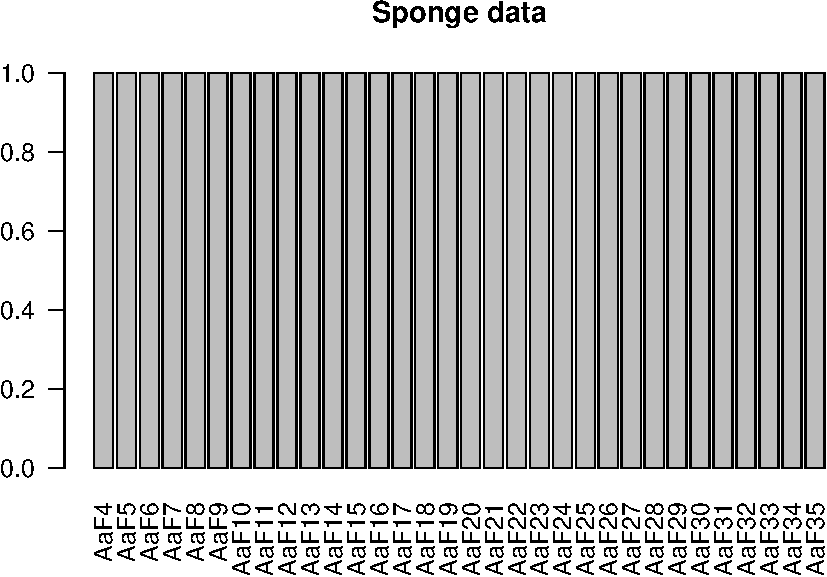
\includegraphics{vignette_files/figure-latex/unnamed-chunk-5-1.pdf}

\begin{Shaded}
\begin{Highlighting}[]
\CommentTok{# ad data}
\NormalTok{ad.lib.size.tss <-}\StringTok{ }\KeywordTok{apply}\NormalTok{(ad.tss, }\DecValTok{1}\NormalTok{, sum)}
\KeywordTok{barplot}\NormalTok{(ad.lib.size.tss, }\DataTypeTok{main =}  \StringTok{'AD data'}\NormalTok{,}\DataTypeTok{las=}\DecValTok{2}\NormalTok{)}
\end{Highlighting}
\end{Shaded}

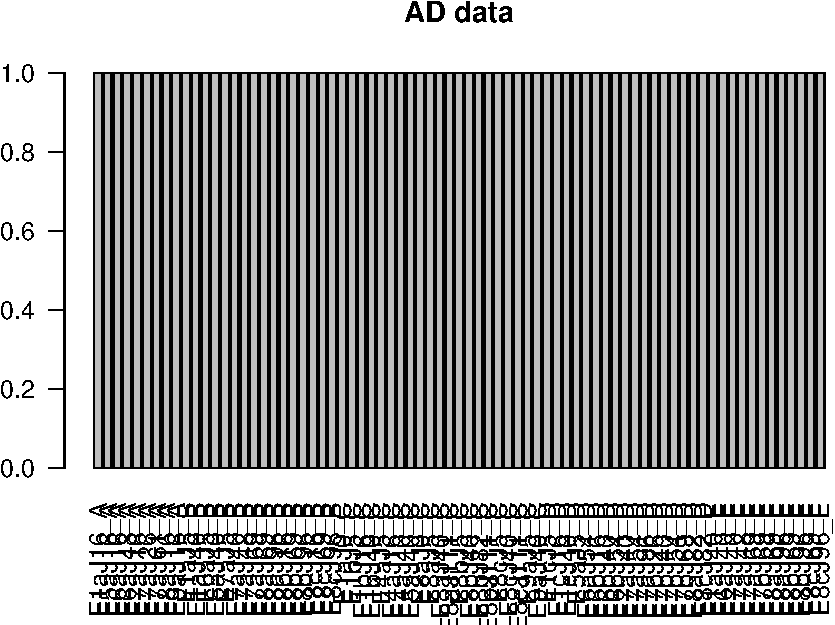
\includegraphics{vignette_files/figure-latex/unnamed-chunk-5-2.pdf}

\begin{Shaded}
\begin{Highlighting}[]
\CommentTok{# hd data}
\NormalTok{hd.lib.size.tss <-}\StringTok{ }\KeywordTok{apply}\NormalTok{(hd.tss, }\DecValTok{1}\NormalTok{, sum)}
\KeywordTok{barplot}\NormalTok{(hd.lib.size.tss, }\DataTypeTok{main =}  \StringTok{'HD data'}\NormalTok{,}\DataTypeTok{las=}\DecValTok{2}\NormalTok{)}
\end{Highlighting}
\end{Shaded}

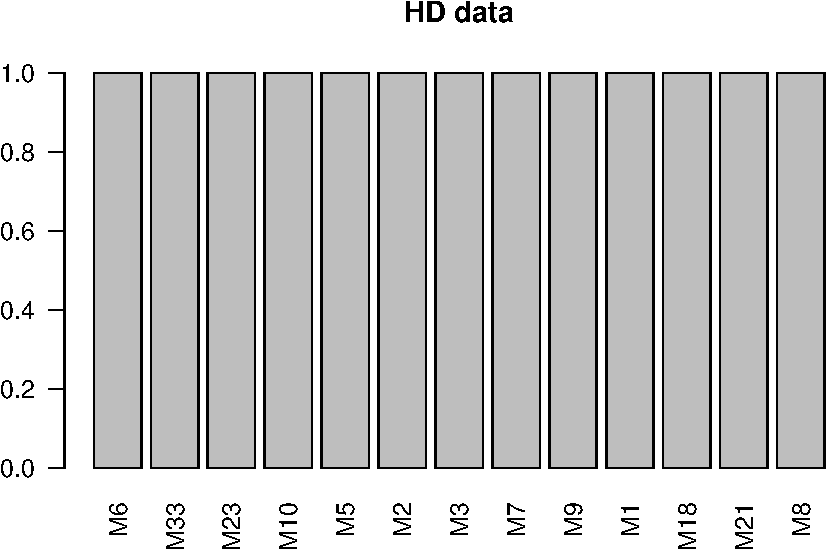
\includegraphics{vignette_files/figure-latex/unnamed-chunk-5-3.pdf}

\subsection{Centered log-ratio
transformation}\label{centered-log-ratio-transformation}

TSS results in compositional data (or proportions) that are restricted
to a space where the sum of all OTU proportions for a given sample sums
to 1. Using standard statistical methods on such data may lead to
spurious results and therefore the data must be further transformed. The
CLR is the transformation of choice.

\begin{Shaded}
\begin{Highlighting}[]
\CommentTok{# sponge data}
\NormalTok{sponge.tss.clr <-}\StringTok{ }\KeywordTok{logratio.transfo}\NormalTok{(sponge.tss,}\DataTypeTok{logratio =} \StringTok{'CLR'}\NormalTok{)}
\KeywordTok{class}\NormalTok{(sponge.tss.clr) <-}\StringTok{ 'matrix'} 

\CommentTok{# ad data}
\NormalTok{ad.tss.clr <-}\StringTok{ }\KeywordTok{logratio.transfo}\NormalTok{(ad.tss,}\DataTypeTok{logratio =} \StringTok{'CLR'}\NormalTok{)}
\KeywordTok{class}\NormalTok{(ad.tss.clr) <-}\StringTok{ 'matrix'} 

\CommentTok{# hd data}
\NormalTok{hd.tss.clr <-}\StringTok{ }\KeywordTok{logratio.transfo}\NormalTok{(hd.tss,}\DataTypeTok{logratio =} \StringTok{'CLR'}\NormalTok{)}
\KeywordTok{class}\NormalTok{(hd.tss.clr) <-}\StringTok{ 'matrix'}
\end{Highlighting}
\end{Shaded}

The final TSS-CLR data of sponge study, AD study and HD study contain 32
samples and 24 OTUs, 75 samples and 231 OTUs, 13 samples and 368 OTUs,
respectively as described in Table 1.

\textbf{Table 1. Overview of exemplar datasets with batch effects.} We
considered microbiome studies from sponge \emph{Aplysina aerophoba};
organic matter in anaerobic digestion (AD) and mice models with
Huntington's disease (HD).

\begin{center}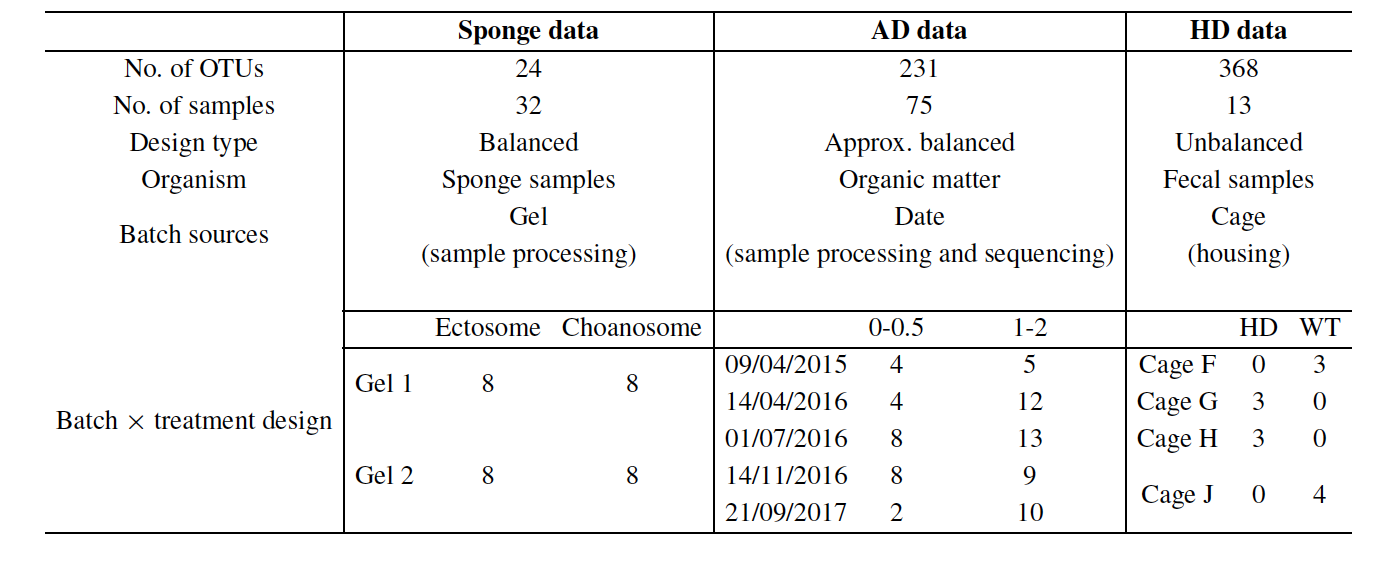
\includegraphics{figures/table} \end{center}

\chapter{Batch effect detection}\label{detect}

In this chapter, we apply qualitative methods to assess the presence of
batch effects using visualisations.

\section{Principal component analysis (PCA) with density plot per
component}\label{principal-component-analysis-pca-with-density-plot-per-component}

We first start with a PCA sample plot with denisty plot per PC.

PCA is an unsupervised method used to explore the data variance
structure by reducing its dimensions to a few principal components (PC)
that explain the greatest variation in the data. Density plots are a
complementary way to visualise batch effects per PC through examining
the distributions of all samples.

\begin{Shaded}
\begin{Highlighting}[]
\CommentTok{# sponge data}
\NormalTok{sponge.pca.before =}\StringTok{ }\KeywordTok{pca}\NormalTok{(sponge.tss.clr, }\DataTypeTok{ncomp =} \DecValTok{3}\NormalTok{)}

\CommentTok{# ad data}
\NormalTok{ad.pca.before =}\StringTok{ }\KeywordTok{pca}\NormalTok{(ad.tss.clr, }\DataTypeTok{ncomp =} \DecValTok{3}\NormalTok{)}

\CommentTok{# hd data}
\NormalTok{hd.pca.before =}\StringTok{ }\KeywordTok{pca}\NormalTok{(hd.tss.clr, }\DataTypeTok{ncomp =} \DecValTok{3}\NormalTok{)}
\end{Highlighting}
\end{Shaded}

The PCA sample plots detect batch effects easily.

\begin{Shaded}
\begin{Highlighting}[]
\KeywordTok{Scatter_Density}\NormalTok{(}\DataTypeTok{data =}\NormalTok{ sponge.pca.before}\OperatorTok{$}\NormalTok{variates}\OperatorTok{$}\NormalTok{X, }\DataTypeTok{batch =}\NormalTok{ sponge.batch, }\DataTypeTok{trt =}\NormalTok{ sponge.trt, }\DataTypeTok{expl.var =}\NormalTok{ sponge.pca.before}\OperatorTok{$}\NormalTok{explained_variance, }\DataTypeTok{xlim =} \KeywordTok{c}\NormalTok{(}\OperatorTok{-}\FloatTok{4.5}\NormalTok{,}\DecValTok{5}\NormalTok{), }\DataTypeTok{ylim =} \KeywordTok{c}\NormalTok{(}\OperatorTok{-}\DecValTok{3}\NormalTok{,}\DecValTok{4}\NormalTok{), }\DataTypeTok{batch.legend.title =} \StringTok{'Gel (batch)'}\NormalTok{, }\DataTypeTok{trt.legend.title =} \StringTok{'Tissue (trt)'}\NormalTok{, }\DataTypeTok{title =} \StringTok{'Before batch effect correction (Sponge)'}\NormalTok{)}
\end{Highlighting}
\end{Shaded}

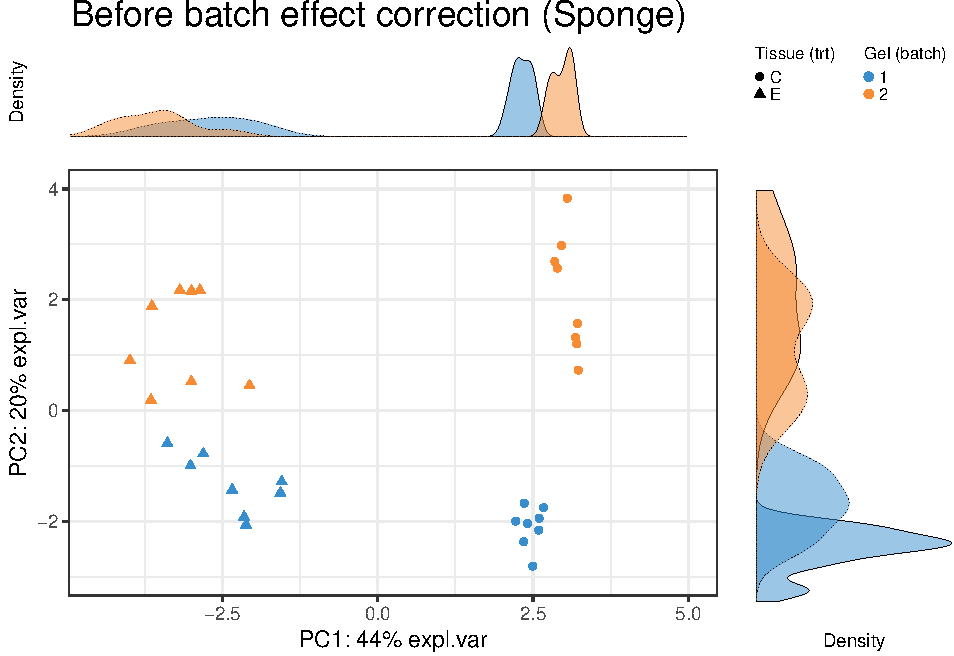
\includegraphics{vignette_files/figure-latex/unnamed-chunk-8-1.pdf}

The first PC (explaining the largest source of variation) shows
variation between samples from different tissues (the effect of
interest), while the second PC (explaining the second largest source of
variation) displays sample differences due to different batches, as also
highlighted in the density plots per component. Therefore, PCA plots can
inform not only of the presence of batch effects, but also which
variation is the largest in the data. In this particular dataset, the
effect of interest variation is larger than batch variation.

\begin{Shaded}
\begin{Highlighting}[]
\KeywordTok{Scatter_Density}\NormalTok{(}\DataTypeTok{data =}\NormalTok{ ad.pca.before}\OperatorTok{$}\NormalTok{variates}\OperatorTok{$}\NormalTok{X, }\DataTypeTok{batch =}\NormalTok{ ad.batch, }\DataTypeTok{trt =}\NormalTok{ ad.trt, }\DataTypeTok{expl.var =}\NormalTok{ ad.pca.before}\OperatorTok{$}\NormalTok{explained_variance, }\DataTypeTok{xlim =} \KeywordTok{c}\NormalTok{(}\OperatorTok{-}\DecValTok{15}\NormalTok{,}\DecValTok{14}\NormalTok{), }\DataTypeTok{ylim =} \KeywordTok{c}\NormalTok{(}\OperatorTok{-}\DecValTok{13}\NormalTok{,}\DecValTok{14}\NormalTok{), }\DataTypeTok{batch.legend.title =} \StringTok{'Date (batch)'}\NormalTok{, }\DataTypeTok{trt.legend.title =} \StringTok{'Conc (trt)'}\NormalTok{, }\DataTypeTok{title =} \StringTok{'Before batch effect correction (AD)'}\NormalTok{)}
\end{Highlighting}
\end{Shaded}

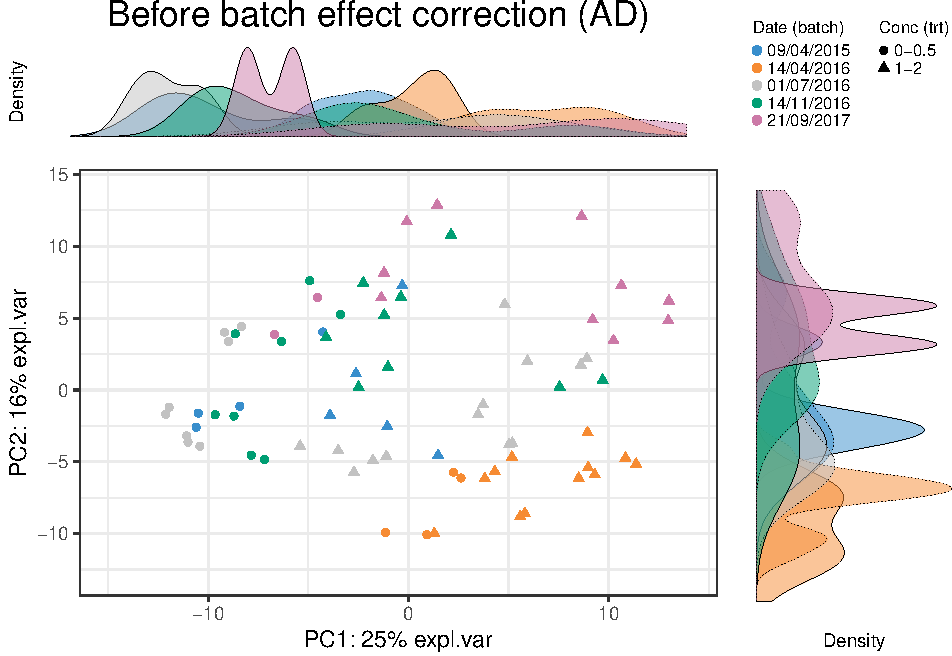
\includegraphics{vignette_files/figure-latex/unnamed-chunk-9-1.pdf}

In AD data, we observe a separation of samples from batch 14/04/2016.

\begin{Shaded}
\begin{Highlighting}[]
\KeywordTok{Scatter_Density}\NormalTok{(}\DataTypeTok{data =}\NormalTok{ hd.pca.before}\OperatorTok{$}\NormalTok{variates}\OperatorTok{$}\NormalTok{X, }\DataTypeTok{batch =}\NormalTok{ hd.batch, }\DataTypeTok{trt =}\NormalTok{ hd.trt, }\DataTypeTok{expl.var =}\NormalTok{ hd.pca.before}\OperatorTok{$}\NormalTok{explained_variance, }\DataTypeTok{xlim =} \KeywordTok{c}\NormalTok{(}\OperatorTok{-}\DecValTok{20}\NormalTok{,}\DecValTok{20}\NormalTok{), }\DataTypeTok{ylim =} \KeywordTok{c}\NormalTok{(}\OperatorTok{-}\DecValTok{25}\NormalTok{,}\DecValTok{15}\NormalTok{), }\DataTypeTok{batch.legend.title =} \StringTok{'Cage (batch)'}\NormalTok{, }\DataTypeTok{trt.legend.title =} \StringTok{'Genotype (trt)'}\NormalTok{, }\DataTypeTok{title =} \StringTok{'Before batch effect correction (HD)'}\NormalTok{)}
\end{Highlighting}
\end{Shaded}

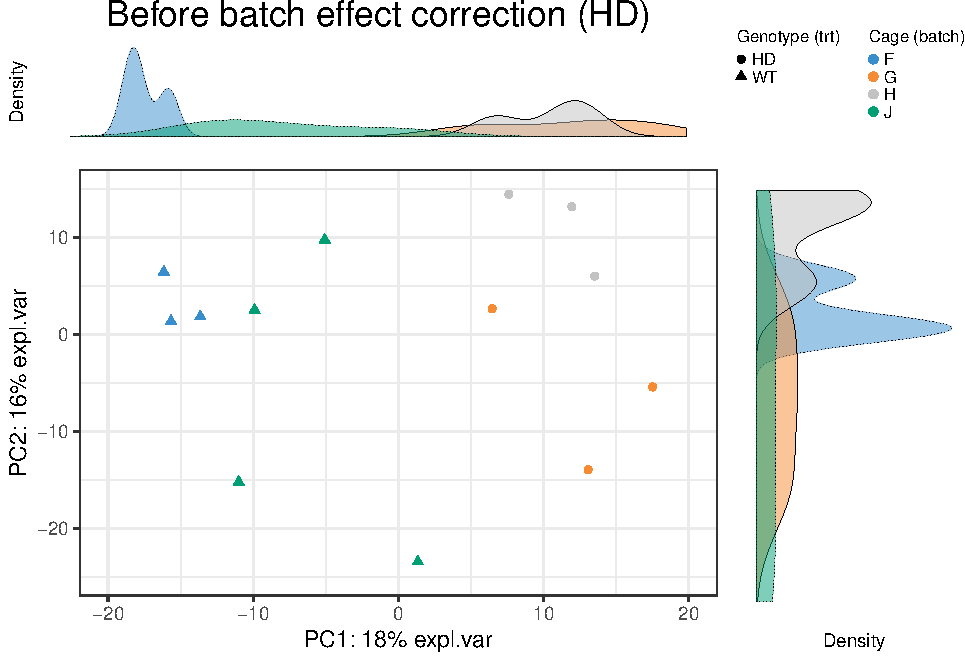
\includegraphics{vignette_files/figure-latex/unnamed-chunk-10-1.pdf}

In HD data, batch effect is due to different cages and obvious.

\section{Density plot and box plot}\label{density-plot-and-box-plot}

We also apply density plots and box plots on OTUs one at a time from
each dataset to visualise batch effects. But only one OTU each dataset
is selected as examples.

For each variable (e.g.~OTU), density plots and box plots can be
generated separately across samples within each batch to observe whether
batch effects serve as a major source of variation.

\begin{Shaded}
\begin{Highlighting}[]
\CommentTok{# sponge data}
\NormalTok{sponge.before.df =}\StringTok{ }\KeywordTok{data.frame}\NormalTok{(}\DataTypeTok{value =}\NormalTok{ sponge.tss.clr[,}\DecValTok{9}\NormalTok{], }\DataTypeTok{batch =}\NormalTok{ sponge.batch)}

\KeywordTok{box_plot_fun}\NormalTok{(}\DataTypeTok{data =}\NormalTok{ sponge.before.df,}\DataTypeTok{x=}\NormalTok{sponge.before.df}\OperatorTok{$}\NormalTok{batch,}
             \DataTypeTok{y=}\NormalTok{sponge.before.df}\OperatorTok{$}\NormalTok{value,}\DataTypeTok{title =} \StringTok{'OTU9 (Sponge)'}\NormalTok{,}
             \DataTypeTok{batch.legend.title =} \StringTok{'Gel (batch)'}\NormalTok{)}
\end{Highlighting}
\end{Shaded}

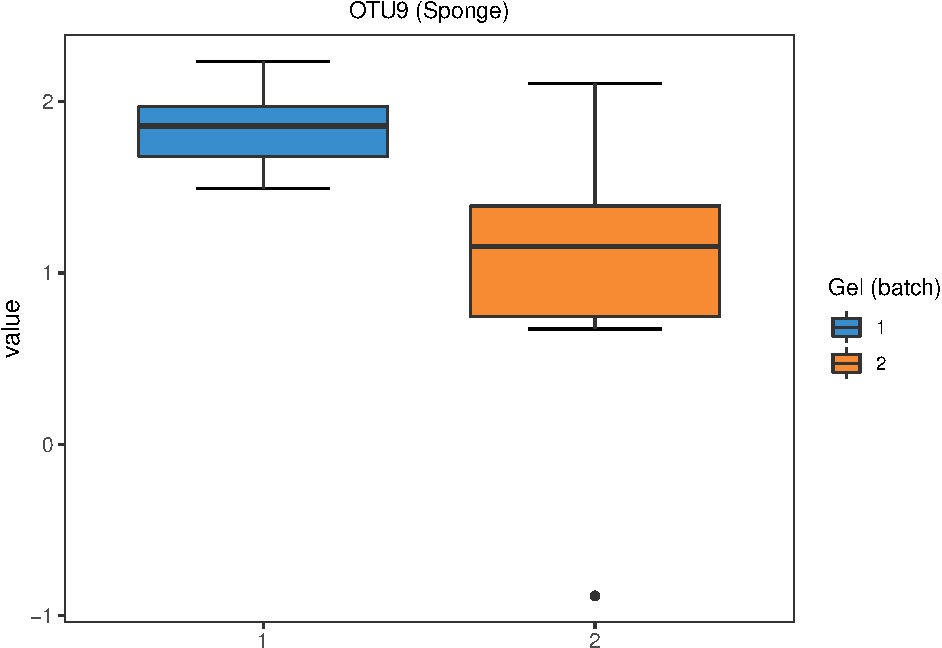
\includegraphics{vignette_files/figure-latex/unnamed-chunk-11-1.pdf}

\begin{Shaded}
\begin{Highlighting}[]
\KeywordTok{ggplot}\NormalTok{(sponge.before.df, }\KeywordTok{aes}\NormalTok{(}\DataTypeTok{x =}\NormalTok{ value, }\DataTypeTok{fill =}\NormalTok{ batch)) }\OperatorTok{+}\StringTok{ }\KeywordTok{geom_density}\NormalTok{(}\DataTypeTok{alpha =} \FloatTok{0.5}\NormalTok{) }\OperatorTok{+}\StringTok{ }\KeywordTok{scale_fill_manual}\NormalTok{(}\DataTypeTok{values=}\KeywordTok{color.mixo}\NormalTok{(}\DecValTok{1}\OperatorTok{:}\DecValTok{10}\NormalTok{)) }\OperatorTok{+}\StringTok{ }\KeywordTok{labs}\NormalTok{(}\DataTypeTok{title =} \StringTok{'OTU9 (Sponge)'}\NormalTok{,}\DataTypeTok{x=}\StringTok{'Value'}\NormalTok{,}\DataTypeTok{fill =} \StringTok{'Gel (batch)'}\NormalTok{) }\OperatorTok{+}\StringTok{ }\KeywordTok{theme_bw}\NormalTok{() }\OperatorTok{+}\StringTok{ }\KeywordTok{theme}\NormalTok{(}\DataTypeTok{plot.title =} \KeywordTok{element_text}\NormalTok{(}\DataTypeTok{hjust=}\FloatTok{0.5}\NormalTok{), }\DataTypeTok{panel.grid =} \KeywordTok{element_blank}\NormalTok{())}
\end{Highlighting}
\end{Shaded}

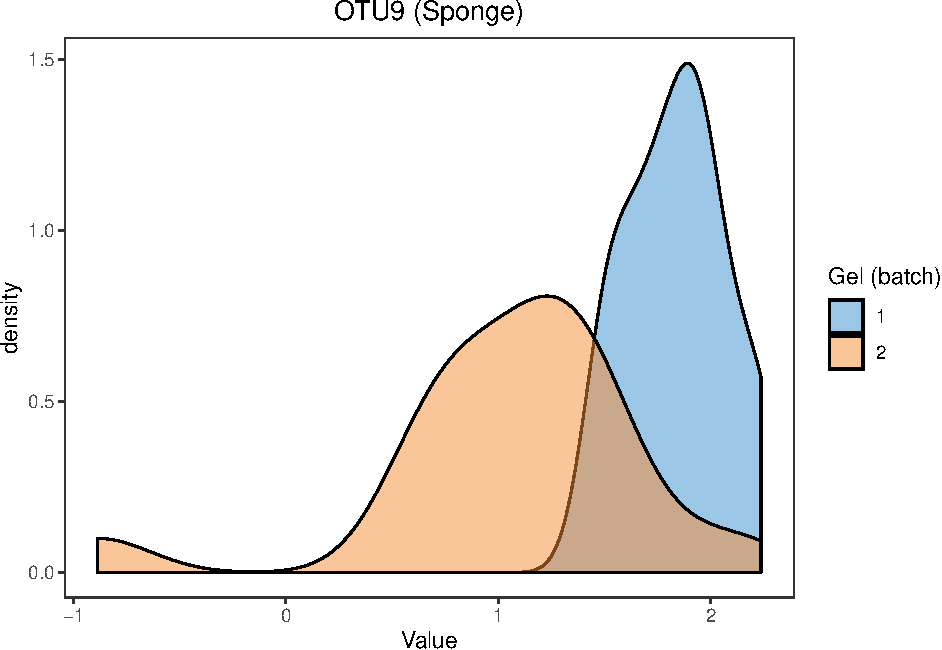
\includegraphics{vignette_files/figure-latex/unnamed-chunk-11-2.pdf}

For the abundance of OTU9, the samples within different batches are very
distinct, indicating a strong batch effect in sponge data.

\begin{Shaded}
\begin{Highlighting}[]
\NormalTok{sponge.lm =}\StringTok{ }\KeywordTok{lm}\NormalTok{(sponge.tss.clr[,}\DecValTok{9}\NormalTok{]}\OperatorTok{~}\StringTok{ }\NormalTok{sponge.trt }\OperatorTok{+}\StringTok{ }\NormalTok{sponge.batch)}
\KeywordTok{summary}\NormalTok{(sponge.lm)}
\end{Highlighting}
\end{Shaded}

\begin{verbatim}
## 
## Call:
## lm(formula = sponge.tss.clr[, 9] ~ sponge.trt + sponge.batch)
## 
## Residuals:
##      Min       1Q   Median       3Q      Max 
## -1.87967 -0.24705  0.04588  0.24492  1.00757 
## 
## Coefficients:
##               Estimate Std. Error t value Pr(>|t|)    
## (Intercept)     1.7849     0.1497  11.922 1.06e-12 ***
## sponge.trtE     0.1065     0.1729   0.616    0.543    
## sponge.batch2  -0.7910     0.1729  -4.575 8.24e-05 ***
## ---
## Signif. codes:  0 '***' 0.001 '**' 0.01 '*' 0.05 '.' 0.1 ' ' 1
## 
## Residual standard error: 0.489 on 29 degrees of freedom
## Multiple R-squared:  0.4236, Adjusted R-squared:  0.3839 
## F-statistic: 10.66 on 2 and 29 DF,  p-value: 0.0003391
\end{verbatim}

The batch effect observed with density and box plots was further
confirmed with a linear regression model with tissue and batch effects
(P \(<\) 0.001 for the regression coefficient associated with the batch
effect in a linear model).

\begin{Shaded}
\begin{Highlighting}[]
\NormalTok{##################}
\CommentTok{# ad data}
\NormalTok{ad.before.df =}\StringTok{ }\KeywordTok{data.frame}\NormalTok{(}\DataTypeTok{value =}\NormalTok{ ad.tss.clr[,}\DecValTok{1}\NormalTok{], }\DataTypeTok{batch =}\NormalTok{ ad.batch)}

\KeywordTok{box_plot_fun}\NormalTok{(}\DataTypeTok{data =}\NormalTok{ ad.before.df,}\DataTypeTok{x=}\NormalTok{ad.before.df}\OperatorTok{$}\NormalTok{batch,}
             \DataTypeTok{y=}\NormalTok{ad.before.df}\OperatorTok{$}\NormalTok{value,}\DataTypeTok{title =} \StringTok{'OTU12 (AD)'}\NormalTok{,}
             \DataTypeTok{batch.legend.title =} \StringTok{'Date (batch)'}\NormalTok{,}
             \DataTypeTok{x.angle =} \DecValTok{45}\NormalTok{, }\DataTypeTok{x.hjust =} \DecValTok{1}\NormalTok{)}
\end{Highlighting}
\end{Shaded}

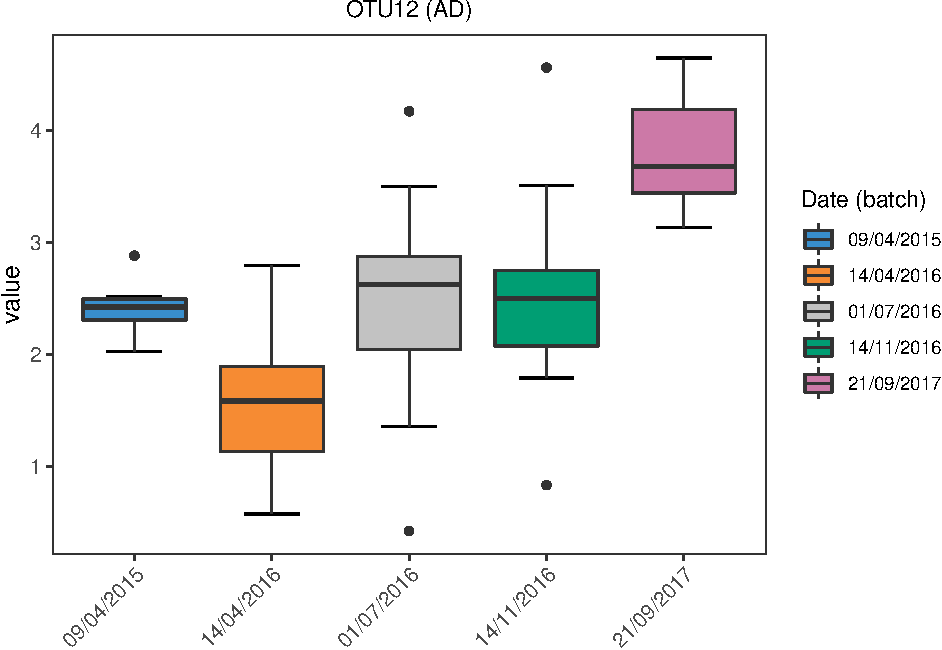
\includegraphics{vignette_files/figure-latex/unnamed-chunk-13-1.pdf}

\begin{Shaded}
\begin{Highlighting}[]
\KeywordTok{ggplot}\NormalTok{(ad.before.df, }\KeywordTok{aes}\NormalTok{(}\DataTypeTok{x =}\NormalTok{ value, }\DataTypeTok{fill =}\NormalTok{ batch)) }\OperatorTok{+}\StringTok{ }\KeywordTok{geom_density}\NormalTok{(}\DataTypeTok{alpha =} \FloatTok{0.5}\NormalTok{) }\OperatorTok{+}\StringTok{ }\KeywordTok{scale_fill_manual}\NormalTok{(}\DataTypeTok{values=}\KeywordTok{color.mixo}\NormalTok{(}\DecValTok{1}\OperatorTok{:}\DecValTok{10}\NormalTok{)) }\OperatorTok{+}\StringTok{ }\KeywordTok{labs}\NormalTok{(}\DataTypeTok{title =} \StringTok{'OTU12 (AD)'}\NormalTok{,}\DataTypeTok{x =} \StringTok{'Value'}\NormalTok{,}\DataTypeTok{fill =} \StringTok{'Date (batch)'}\NormalTok{) }\OperatorTok{+}\StringTok{ }\KeywordTok{theme_bw}\NormalTok{() }\OperatorTok{+}\StringTok{ }\KeywordTok{theme}\NormalTok{(}\DataTypeTok{plot.title =} \KeywordTok{element_text}\NormalTok{(}\DataTypeTok{hjust=}\FloatTok{0.5}\NormalTok{), }\DataTypeTok{panel.grid =} \KeywordTok{element_blank}\NormalTok{())}
\end{Highlighting}
\end{Shaded}

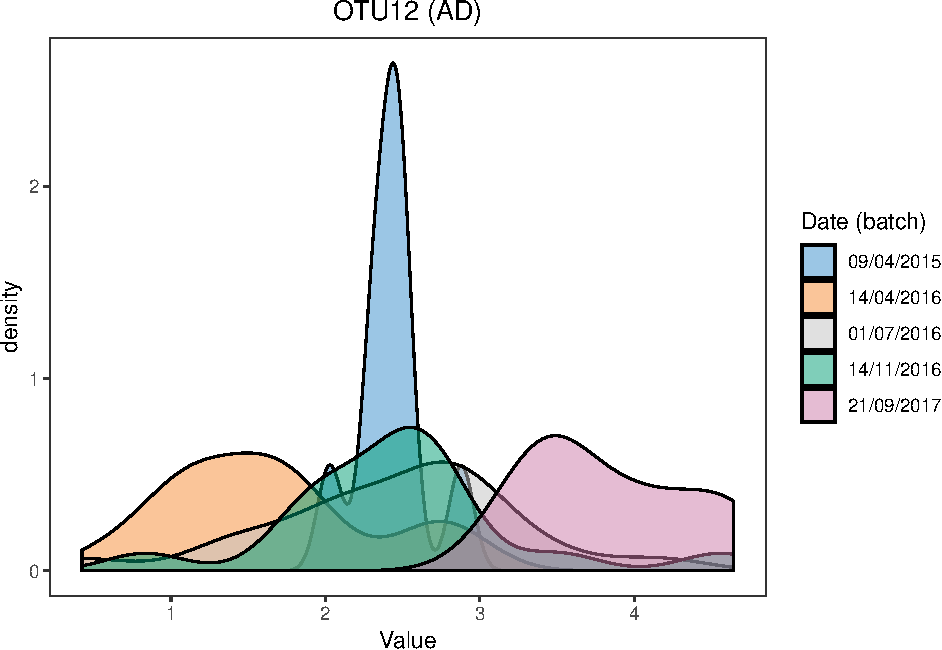
\includegraphics{vignette_files/figure-latex/unnamed-chunk-13-2.pdf}

Batch effects in AD data are also visualised.

\begin{Shaded}
\begin{Highlighting}[]
\NormalTok{ad.lm =}\StringTok{ }\KeywordTok{lm}\NormalTok{(ad.tss.clr[,}\DecValTok{1}\NormalTok{]}\OperatorTok{~}\StringTok{ }\NormalTok{ad.trt }\OperatorTok{+}\StringTok{ }\NormalTok{ad.batch)}
\KeywordTok{anova}\NormalTok{(ad.lm)}
\end{Highlighting}
\end{Shaded}

\begin{verbatim}
## Analysis of Variance Table
## 
## Response: ad.tss.clr[, 1]
##           Df Sum Sq Mean Sq F value    Pr(>F)    
## ad.trt     1  1.460  1.4605  3.1001   0.08272 .  
## ad.batch   4 32.889  8.2222 17.4532 6.168e-10 ***
## Residuals 69 32.506  0.4711                      
## ---
## Signif. codes:  0 '***' 0.001 '**' 0.01 '*' 0.05 '.' 0.1 ' ' 1
\end{verbatim}

The difference between batches is statistically significant (P
\textless{} 0.001, as tested with ANOVA). We can also obtain P values
between each two batch categories.

\begin{Shaded}
\begin{Highlighting}[]
\KeywordTok{summary}\NormalTok{(ad.lm)}
\end{Highlighting}
\end{Shaded}

\begin{verbatim}
## 
## Call:
## lm(formula = ad.tss.clr[, 1] ~ ad.trt + ad.batch)
## 
## Residuals:
##      Min       1Q   Median       3Q      Max 
## -2.09885 -0.39613 -0.00381  0.36645  1.98185 
## 
## Coefficients:
##                     Estimate Std. Error t value Pr(>|t|)    
## (Intercept)         2.311213   0.247768   9.328 7.57e-14 ***
## ad.trt1-2           0.203619   0.171183   1.189  0.23833    
## ad.batch14/04/2016 -0.828100   0.287918  -2.876  0.00535 ** 
## ad.batch01/07/2016  0.007239   0.273672   0.026  0.97897    
## ad.batch14/11/2016  0.062689   0.282978   0.222  0.82533    
## ad.batch21/09/2017  1.361132   0.306373   4.443 3.30e-05 ***
## ---
## Signif. codes:  0 '***' 0.001 '**' 0.01 '*' 0.05 '.' 0.1 ' ' 1
## 
## Residual standard error: 0.6864 on 69 degrees of freedom
## Multiple R-squared:  0.5138, Adjusted R-squared:  0.4786 
## F-statistic: 14.58 on 5 and 69 DF,  p-value: 9.665e-10
\end{verbatim}

\begin{Shaded}
\begin{Highlighting}[]
\NormalTok{##################}
\CommentTok{# hd data}
\NormalTok{hd.before.df =}\StringTok{ }\KeywordTok{data.frame}\NormalTok{(}\DataTypeTok{value =}\NormalTok{ hd.tss.clr[,}\DecValTok{1}\NormalTok{], }\DataTypeTok{batch =}\NormalTok{ hd.batch)}

\KeywordTok{box_plot_fun}\NormalTok{(}\DataTypeTok{data =}\NormalTok{ hd.before.df,}\DataTypeTok{x=}\NormalTok{hd.before.df}\OperatorTok{$}\NormalTok{batch,}
             \DataTypeTok{y=}\NormalTok{hd.before.df}\OperatorTok{$}\NormalTok{value,}\DataTypeTok{title =} \StringTok{'OTU1 (HD)'}\NormalTok{,}
             \DataTypeTok{batch.legend.title =} \StringTok{'Cage (batch)'}\NormalTok{)}
\end{Highlighting}
\end{Shaded}

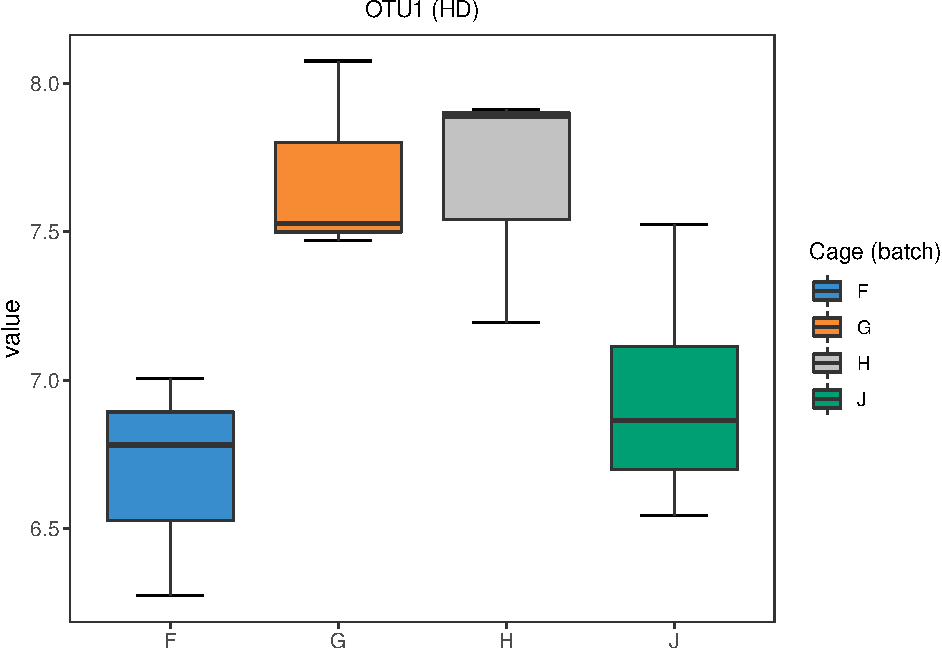
\includegraphics{vignette_files/figure-latex/unnamed-chunk-16-1.pdf}

\begin{Shaded}
\begin{Highlighting}[]
\KeywordTok{ggplot}\NormalTok{(hd.before.df, }\KeywordTok{aes}\NormalTok{(}\DataTypeTok{x =}\NormalTok{ value, }\DataTypeTok{fill =}\NormalTok{ batch)) }\OperatorTok{+}\StringTok{ }\KeywordTok{geom_density}\NormalTok{(}\DataTypeTok{alpha =} \FloatTok{0.5}\NormalTok{) }\OperatorTok{+}\StringTok{ }\KeywordTok{scale_fill_manual}\NormalTok{(}\DataTypeTok{values=}\KeywordTok{color.mixo}\NormalTok{(}\DecValTok{1}\OperatorTok{:}\DecValTok{10}\NormalTok{)) }\OperatorTok{+}\StringTok{ }\KeywordTok{labs}\NormalTok{(}\DataTypeTok{title =} \StringTok{'OTU1 (HD)'}\NormalTok{,}\DataTypeTok{x =} \StringTok{'Value'}\NormalTok{,}\DataTypeTok{fill =} \StringTok{'Cage (batch)'}\NormalTok{) }\OperatorTok{+}\StringTok{ }\KeywordTok{theme_bw}\NormalTok{() }\OperatorTok{+}\StringTok{ }\KeywordTok{theme}\NormalTok{(}\DataTypeTok{plot.title =} \KeywordTok{element_text}\NormalTok{(}\DataTypeTok{hjust=}\FloatTok{0.5}\NormalTok{), }\DataTypeTok{panel.grid =} \KeywordTok{element_blank}\NormalTok{())}
\end{Highlighting}
\end{Shaded}

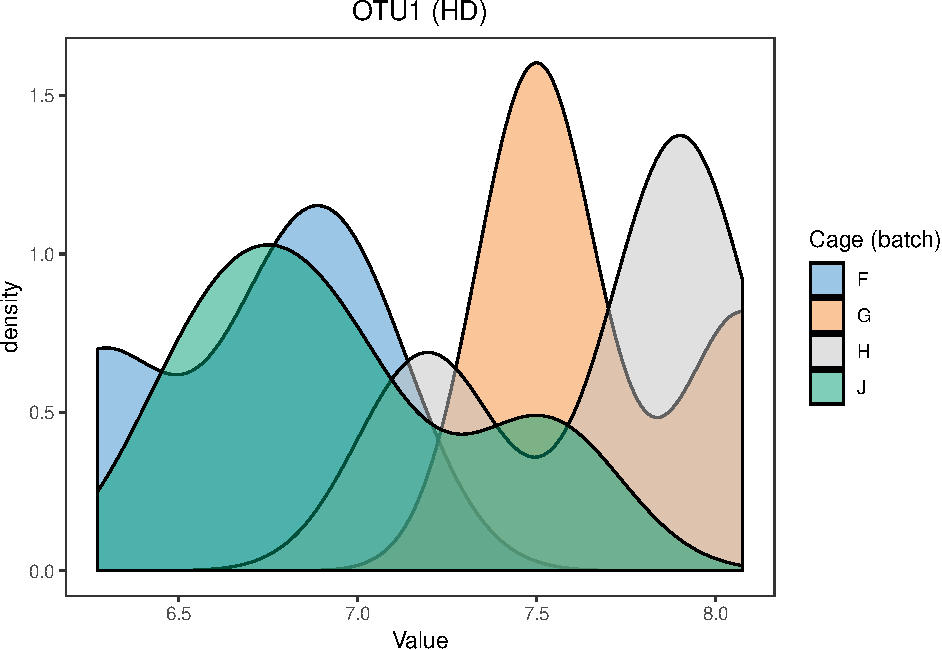
\includegraphics{vignette_files/figure-latex/unnamed-chunk-16-2.pdf}

It is easy to detect the differences between samples within different
batches.

\begin{Shaded}
\begin{Highlighting}[]
\NormalTok{hd.lm =}\StringTok{ }\KeywordTok{lm}\NormalTok{(hd.tss.clr[,}\DecValTok{1}\NormalTok{]}\OperatorTok{~}\StringTok{ }\NormalTok{hd.batch)}
\KeywordTok{anova}\NormalTok{(hd.lm)}
\end{Highlighting}
\end{Shaded}

\begin{verbatim}
## Analysis of Variance Table
## 
## Response: hd.tss.clr[, 1]
##           Df Sum Sq Mean Sq F value  Pr(>F)  
## hd.batch   3 2.4108 0.80359  5.2569 0.02276 *
## Residuals  9 1.3758 0.15286                  
## ---
## Signif. codes:  0 '***' 0.001 '**' 0.01 '*' 0.05 '.' 0.1 ' ' 1
\end{verbatim}

As the batch \(\times\) treatment design of HD data is nested and
unbalanced, the linear model with both treatment (genotype) and batch
(cage) is unable to fit. We therefore fit a linear model with batch
effect only. The difference between cages is statistically significant
(P \textless{} 0.05). But the difference may also be influenced by
treatment and we are unable to exclude this influence.

\section{RLE plots}\label{rle-plots}

RLE plots can be plotted using `RleMicroRna' in R package `AgiMicroRna'.
Here, we made some changes on the function `RleMicroRna', thus we call
it `RleMicroRna2'.

RLE plots are based on the assumption that the majority of microbial
variables are unaffected by the effect of interest, and therefore any
sample heterogeneity observed - i.e.~different distributions and their
variances, and medians different from zero, should indicate the presence
of batch effects. In our case studies, the treatment information is
known, so we generate multiple RLE plots per treatment group, as
suggested by \citep{lin2018scmerge}.

\begin{Shaded}
\begin{Highlighting}[]
\CommentTok{# sponge data}
\NormalTok{sponge.batch_c =}\StringTok{ }\NormalTok{sponge.batch[sponge.trt }\OperatorTok{==}\StringTok{ 'C'}\NormalTok{]}
\NormalTok{sponge.batch_e =}\StringTok{ }\NormalTok{sponge.batch[sponge.trt }\OperatorTok{==}\StringTok{ 'E'}\NormalTok{] }

\CommentTok{# before}
\NormalTok{sponge.before_c =}\StringTok{ }\NormalTok{sponge.tss.clr[sponge.trt }\OperatorTok{==}\StringTok{ 'C'}\NormalTok{,]}
\NormalTok{sponge.before_e =}\StringTok{ }\NormalTok{sponge.tss.clr[sponge.trt }\OperatorTok{==}\StringTok{ 'E'}\NormalTok{,] }


\KeywordTok{RleMicroRna2}\NormalTok{(}\DataTypeTok{object =} \KeywordTok{t}\NormalTok{(sponge.before_c),}\DataTypeTok{batch =}\NormalTok{ sponge.batch_c,}\DataTypeTok{maintitle =} \StringTok{'Sponge (tissue: choanosome)'}\NormalTok{)}
\end{Highlighting}
\end{Shaded}

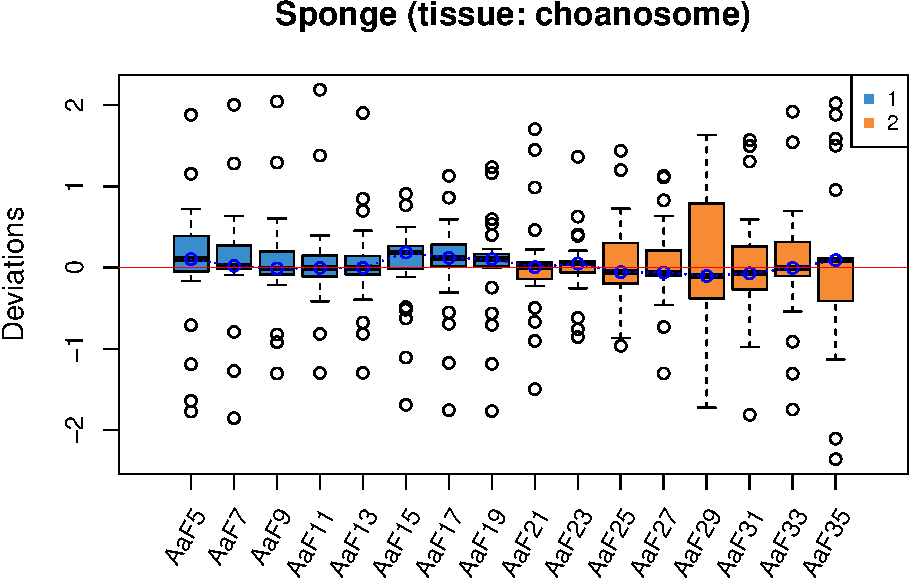
\includegraphics{vignette_files/figure-latex/unnamed-chunk-18-1.pdf}

\begin{Shaded}
\begin{Highlighting}[]
\KeywordTok{RleMicroRna2}\NormalTok{(}\DataTypeTok{object =} \KeywordTok{t}\NormalTok{(sponge.before_e),}\DataTypeTok{batch =}\NormalTok{ sponge.batch_e,}\DataTypeTok{maintitle =} \StringTok{'Sponge (tissue: ectosome)'}\NormalTok{)}
\end{Highlighting}
\end{Shaded}

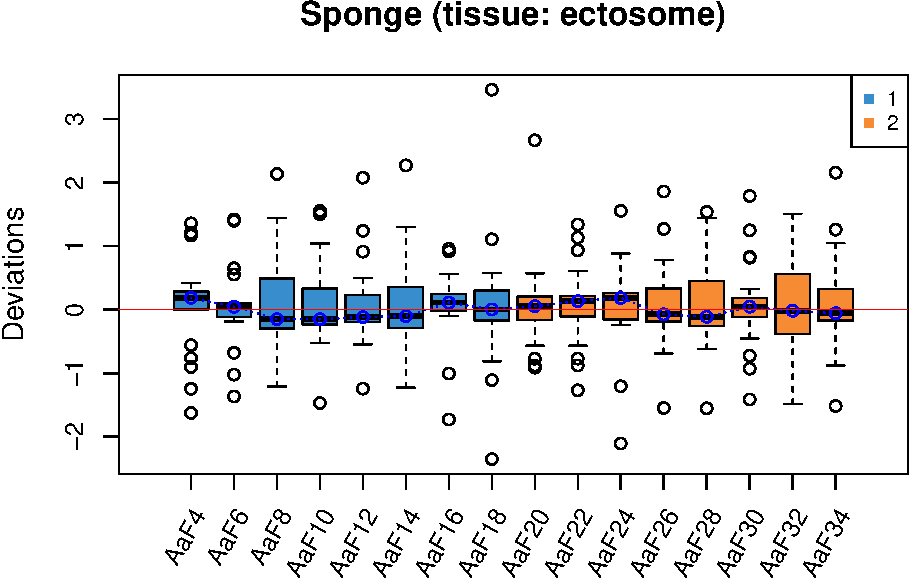
\includegraphics{vignette_files/figure-latex/unnamed-chunk-18-2.pdf}

The batch effect before correction is not obvious as all medians of
samples are close to zero, but Gel2 has a greater interquartile range
(IQR) than the other samples.

\begin{Shaded}
\begin{Highlighting}[]
\CommentTok{# ad data}
\NormalTok{ad.batch_}\DecValTok{05}\NormalTok{ =}\StringTok{ }\NormalTok{ad.batch[ad.trt }\OperatorTok{==}\StringTok{ '0-0.5'}\NormalTok{]}
\NormalTok{ad.batch_}\DecValTok{2}\NormalTok{ =}\StringTok{ }\NormalTok{ad.batch[ad.trt }\OperatorTok{==}\StringTok{ '1-2'}\NormalTok{] }

\CommentTok{# before}
\NormalTok{ad.before_}\DecValTok{05}\NormalTok{ =}\StringTok{ }\NormalTok{ad.tss.clr[ad.trt }\OperatorTok{==}\StringTok{ '0-0.5'}\NormalTok{,]}
\NormalTok{ad.before_}\DecValTok{2}\NormalTok{ =}\StringTok{ }\NormalTok{ad.tss.clr[ad.trt }\OperatorTok{==}\StringTok{ '1-2'}\NormalTok{,]}

\KeywordTok{RleMicroRna2}\NormalTok{(}\DataTypeTok{object =} \KeywordTok{t}\NormalTok{(ad.before_}\DecValTok{05}\NormalTok{),}\DataTypeTok{batch =}\NormalTok{ ad.batch_}\DecValTok{05}\NormalTok{,}\DataTypeTok{maintitle =} \StringTok{'AD (initial phenol conc: 0-0.5 g/L)'}\NormalTok{,}\DataTypeTok{legend.cex =} \FloatTok{0.5}\NormalTok{)}
\end{Highlighting}
\end{Shaded}

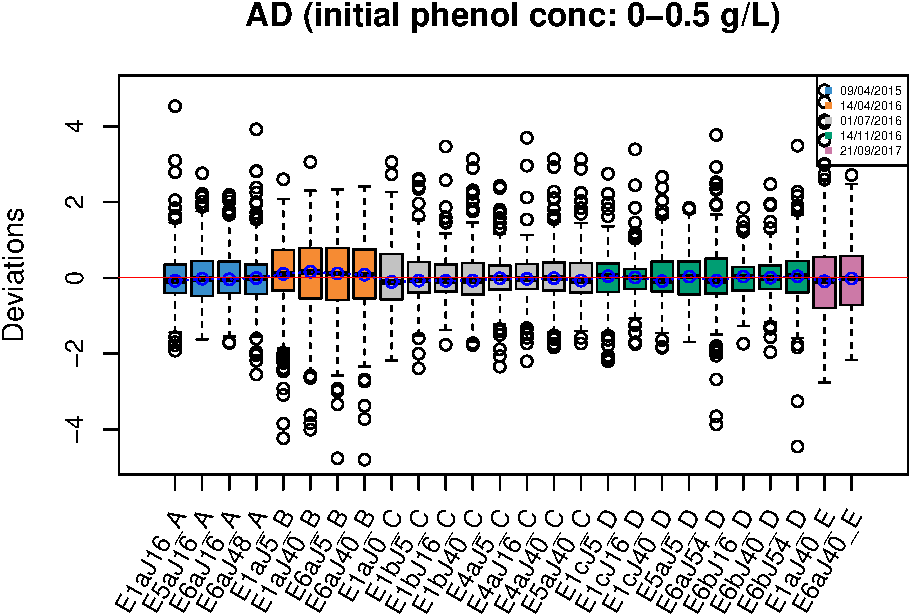
\includegraphics{vignette_files/figure-latex/unnamed-chunk-19-1.pdf}

\begin{Shaded}
\begin{Highlighting}[]
\KeywordTok{RleMicroRna2}\NormalTok{(}\DataTypeTok{object =} \KeywordTok{t}\NormalTok{(ad.before_}\DecValTok{2}\NormalTok{),}\DataTypeTok{batch =}\NormalTok{ ad.batch_}\DecValTok{2}\NormalTok{,}\DataTypeTok{maintitle =} \StringTok{'AD (initial phenol conc: 1-2 g/L)'}\NormalTok{,}\DataTypeTok{cex.xaxis =} \FloatTok{0.7}\NormalTok{,}\DataTypeTok{legend.cex =} \FloatTok{0.5}\NormalTok{)}
\end{Highlighting}
\end{Shaded}

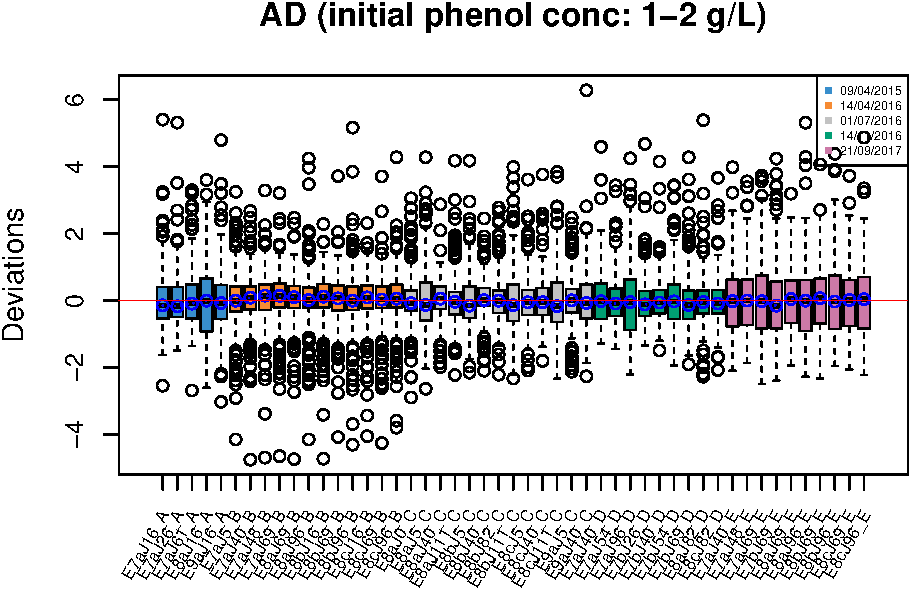
\includegraphics{vignette_files/figure-latex/unnamed-chunk-19-2.pdf}

In RLE plots for the AD data, the batch effect before correction is not
obvious as all medians of samples are close to zero, but the samples
dated 14/04/2016 may be affected by batch.

\begin{Shaded}
\begin{Highlighting}[]
\CommentTok{# hd data ###########}
\NormalTok{hd.batch_h =}\StringTok{ }\NormalTok{hd.batch[hd.trt }\OperatorTok{==}\StringTok{ 'HD'}\NormalTok{]}
\NormalTok{hd.batch_w =}\StringTok{ }\NormalTok{hd.batch[hd.trt }\OperatorTok{==}\StringTok{ 'WT'}\NormalTok{] }

\CommentTok{# before}
\NormalTok{hd.before_h =}\StringTok{ }\NormalTok{hd.tss.clr[hd.trt }\OperatorTok{==}\StringTok{ 'HD'}\NormalTok{,]}
\NormalTok{hd.before_w =}\StringTok{ }\NormalTok{hd.tss.clr[hd.trt }\OperatorTok{==}\StringTok{ 'WT'}\NormalTok{,]}

\KeywordTok{RleMicroRna2}\NormalTok{(}\DataTypeTok{object =} \KeywordTok{t}\NormalTok{(hd.before_h),}\DataTypeTok{batch =}\NormalTok{ hd.batch_h,}\DataTypeTok{maintitle =} \StringTok{'HD (genotype: HD)'}\NormalTok{)}
\end{Highlighting}
\end{Shaded}

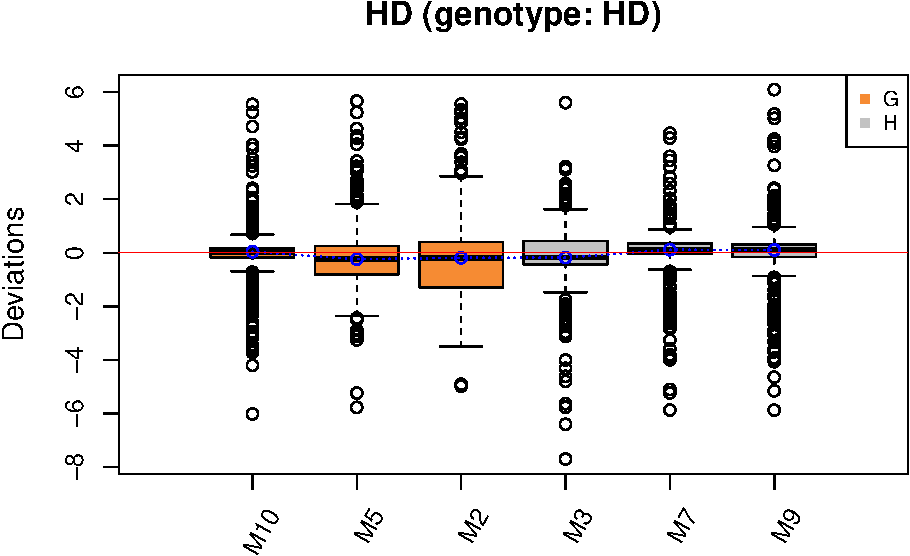
\includegraphics{vignette_files/figure-latex/unnamed-chunk-20-1.pdf}

\begin{Shaded}
\begin{Highlighting}[]
\KeywordTok{RleMicroRna2}\NormalTok{(}\DataTypeTok{object =} \KeywordTok{t}\NormalTok{(hd.before_w),}\DataTypeTok{batch =}\NormalTok{ hd.batch_w,}\DataTypeTok{maintitle =} \StringTok{'HD (genotype: WT)'}\NormalTok{)}
\end{Highlighting}
\end{Shaded}

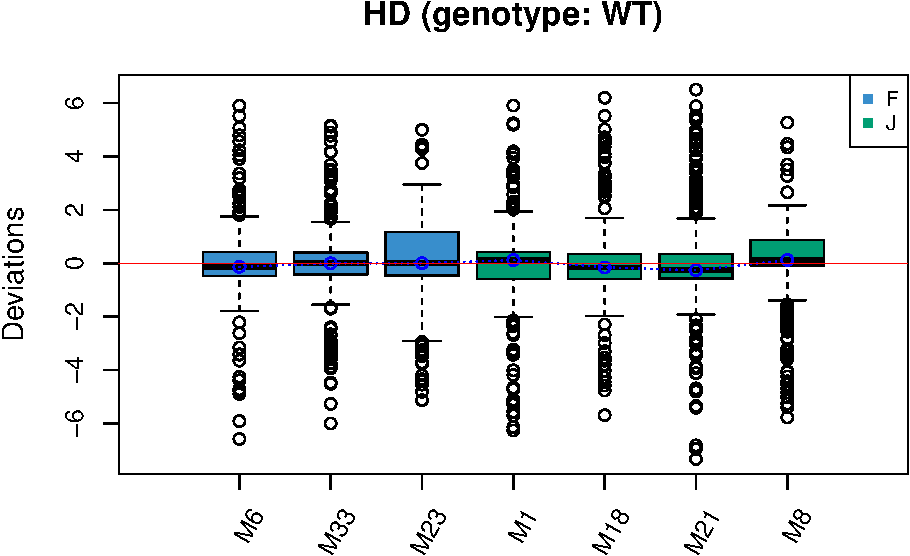
\includegraphics{vignette_files/figure-latex/unnamed-chunk-20-2.pdf} The
batch effect in HD data is not easily detected, but Cage G has a greater
interquartile range (IQR) than the other samples, which may indicate a
batch effect.

\section{Heatmap}\label{heatmap}

Clustering analysis can be used to detect batch effects. Ideally samples
with the same treatment will be clustered together, data clustered by
batches instead of treatments indicate a batch effect. Heatmaps and
dendrograms are two common approaches to visualise the clusters.

\begin{Shaded}
\begin{Highlighting}[]
\CommentTok{# Sponge data}
\CommentTok{#scale }
\NormalTok{sponge.tss.clr.scale =}\StringTok{ }\KeywordTok{scale}\NormalTok{(sponge.tss.clr,}\DataTypeTok{center =}\NormalTok{ T, }\DataTypeTok{scale =}\NormalTok{ T) }\CommentTok{# scale on OTUs}
\NormalTok{sponge.tss.clr.scale =}\StringTok{ }\KeywordTok{scale}\NormalTok{(}\KeywordTok{t}\NormalTok{(sponge.tss.clr.scale), }\DataTypeTok{center =}\NormalTok{ T, }\DataTypeTok{scale =}\NormalTok{ T) }\CommentTok{# scale on samples}

\NormalTok{sponge.anno_col =}\StringTok{ }\KeywordTok{data.frame}\NormalTok{(}\DataTypeTok{Batch =}\NormalTok{ sponge.batch, }\DataTypeTok{Tissue =}\NormalTok{ sponge.trt)}
\NormalTok{sponge.anno_metabo_colors =}\StringTok{ }\KeywordTok{list}\NormalTok{(}\DataTypeTok{Batch =} \KeywordTok{c}\NormalTok{(}\StringTok{'1'}\NormalTok{=}\StringTok{"#388ECC"}\NormalTok{,}\StringTok{'2'}\NormalTok{=}\StringTok{"#F68B33"}\NormalTok{),}\DataTypeTok{Tissue =} \KeywordTok{c}\NormalTok{(}\DataTypeTok{C=}\StringTok{"#F0E442"}\NormalTok{,}\DataTypeTok{E=}\StringTok{"#D55E00"}\NormalTok{))}


\KeywordTok{pheatmap}\NormalTok{(sponge.tss.clr.scale, }
         \DataTypeTok{scale =} \StringTok{'none'}\NormalTok{, }
         \DataTypeTok{cluster_rows =}\NormalTok{ F, }
         \DataTypeTok{cluster_cols =}\NormalTok{ T, }
         \DataTypeTok{fontsize_row=}\DecValTok{5}\NormalTok{, }\DataTypeTok{fontsize_col=}\DecValTok{8}\NormalTok{,}
         \DataTypeTok{fontsize =} \DecValTok{8}\NormalTok{,}
         \DataTypeTok{clustering_distance_rows =} \StringTok{"euclidean"}\NormalTok{,}
         \DataTypeTok{clustering_method =} \StringTok{"ward.D"}\NormalTok{,}
         \DataTypeTok{treeheight_row =} \DecValTok{30}\NormalTok{,}
         \DataTypeTok{annotation_col =}\NormalTok{ sponge.anno_col,}
         \DataTypeTok{annotation_colors =}\NormalTok{ sponge.anno_metabo_colors,}
         \DataTypeTok{border_color =} \StringTok{'NA'}\NormalTok{,}
         \DataTypeTok{main =} \StringTok{'Sponge data - Scaled'}\NormalTok{)}
\end{Highlighting}
\end{Shaded}

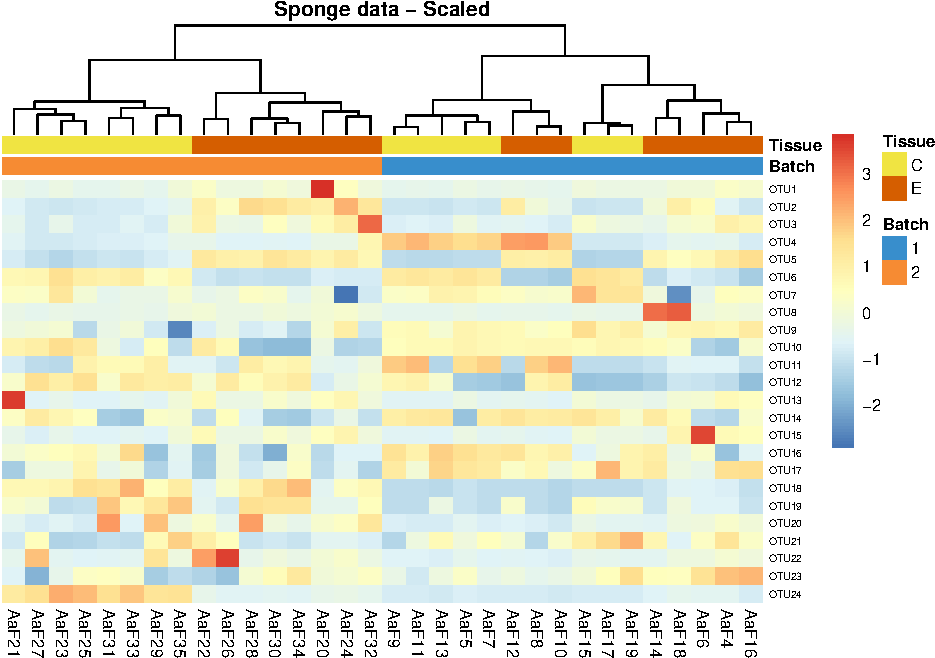
\includegraphics{vignette_files/figure-latex/unnamed-chunk-21-1.pdf}

In sponge data, samples are preferentially clustered by batch instead of
tissue type, indicating a batch effect.

\begin{Shaded}
\begin{Highlighting}[]
\NormalTok{#################}
\CommentTok{# AD data}
\CommentTok{#scale }
\NormalTok{ad.tss.clr.scale =}\StringTok{ }\KeywordTok{scale}\NormalTok{(ad.tss.clr,}\DataTypeTok{center =}\NormalTok{ T, }\DataTypeTok{scale =}\NormalTok{ T) }\CommentTok{# scale on OTUs}
\NormalTok{ad.tss.clr.scale =}\StringTok{ }\KeywordTok{scale}\NormalTok{(}\KeywordTok{t}\NormalTok{(ad.tss.clr.scale), }\DataTypeTok{center =}\NormalTok{ T, }\DataTypeTok{scale =}\NormalTok{ T) }\CommentTok{# scale on samples}

\NormalTok{ad.anno_col =}\StringTok{ }\KeywordTok{data.frame}\NormalTok{(}\DataTypeTok{Batch =}\NormalTok{ ad.batch, }\DataTypeTok{Treatment =}\NormalTok{ ad.trt)}
\NormalTok{ad.anno_metabo_colors =}\StringTok{ }\KeywordTok{list}\NormalTok{(}\DataTypeTok{Batch =} \KeywordTok{c}\NormalTok{(}\StringTok{'09/04/2015'}\NormalTok{=}\StringTok{"#388ECC"}\NormalTok{,}\StringTok{'14/04/2016'}\NormalTok{=}\StringTok{"#F68B33"}\NormalTok{,}\StringTok{'01/07/2016'}\NormalTok{=}\StringTok{"#C2C2C2"}\NormalTok{,}\StringTok{'14/11/2016'}\NormalTok{=}\StringTok{"#009E73"}\NormalTok{,}\StringTok{'21/09/2017'}\NormalTok{=}\StringTok{"#CC79A7"}\NormalTok{), }\DataTypeTok{Treatment =} \KeywordTok{c}\NormalTok{(}\StringTok{"0-0.5"}\NormalTok{ =}\StringTok{ "#0072B2"}\NormalTok{, }\StringTok{"1-2"}\NormalTok{ =}\StringTok{ "#999999"}\NormalTok{))}


\KeywordTok{pheatmap}\NormalTok{(ad.tss.clr.scale, }
         \DataTypeTok{scale =} \StringTok{'none'}\NormalTok{, }
         \DataTypeTok{cluster_rows =}\NormalTok{ F, }
         \DataTypeTok{cluster_cols =}\NormalTok{ T, }
         \DataTypeTok{fontsize_row=}\DecValTok{4}\NormalTok{, }\DataTypeTok{fontsize_col=}\DecValTok{6}\NormalTok{,}
         \DataTypeTok{fontsize =} \DecValTok{8}\NormalTok{,}
         \DataTypeTok{clustering_distance_rows =} \StringTok{"euclidean"}\NormalTok{,}
         \DataTypeTok{clustering_method =} \StringTok{"ward.D"}\NormalTok{,}
         \DataTypeTok{treeheight_row =} \DecValTok{30}\NormalTok{,}
         \DataTypeTok{annotation_col =}\NormalTok{ ad.anno_col,}
         \DataTypeTok{annotation_colors=}\NormalTok{ ad.anno_metabo_colors,}
         \DataTypeTok{border_color =} \StringTok{'NA'}\NormalTok{,}
         \DataTypeTok{main =} \StringTok{'AD data - Scaled'}\NormalTok{)}
\end{Highlighting}
\end{Shaded}

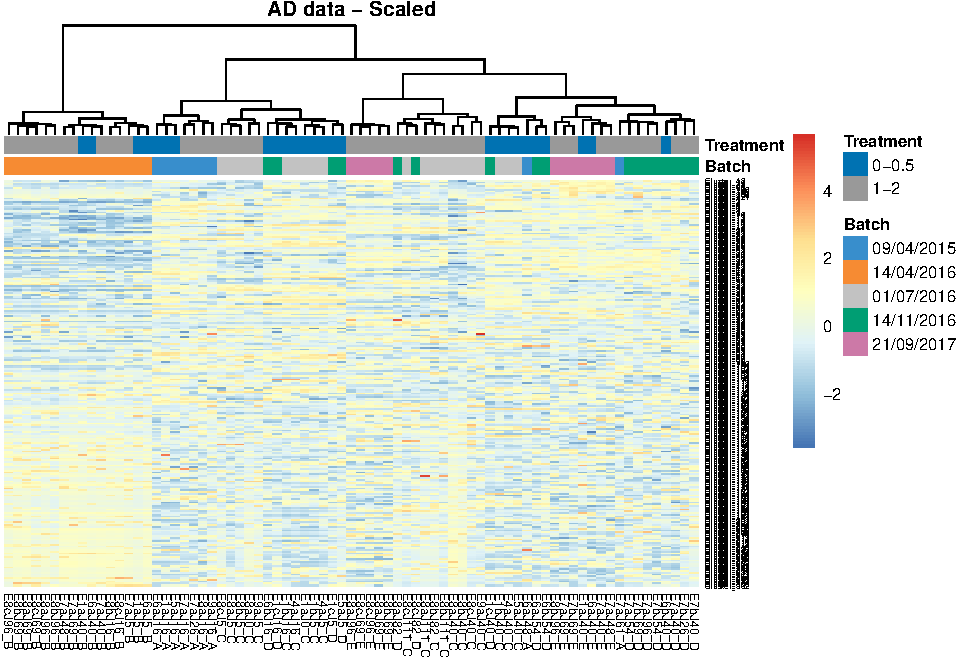
\includegraphics{vignette_files/figure-latex/unnamed-chunk-22-1.pdf}

In AD data, samples within batch 14/04/2016 are clustered and distinct
from other samples, also indicating a batch effect.

\begin{Shaded}
\begin{Highlighting}[]
\NormalTok{#################}
\CommentTok{# HD data}
\CommentTok{#scale }
\NormalTok{hd.tss.clr.scale =}\StringTok{ }\KeywordTok{scale}\NormalTok{(hd.tss.clr,}\DataTypeTok{center =}\NormalTok{ T, }\DataTypeTok{scale =}\NormalTok{ T) }\CommentTok{# scale on OTUs}
\NormalTok{hd.tss.clr.scale =}\StringTok{ }\KeywordTok{scale}\NormalTok{(}\KeywordTok{t}\NormalTok{(hd.tss.clr.scale), }\DataTypeTok{center =}\NormalTok{ T, }\DataTypeTok{scale =}\NormalTok{ T) }\CommentTok{# scale on samples}

\NormalTok{hd.anno_col =}\StringTok{ }\KeywordTok{data.frame}\NormalTok{(}\DataTypeTok{Batch =}\NormalTok{ hd.batch, }\DataTypeTok{Treatment =}\NormalTok{ hd.trt)}
\NormalTok{hd.anno_metabo_colors =}\StringTok{ }\KeywordTok{list}\NormalTok{(}\DataTypeTok{Batch =} \KeywordTok{c}\NormalTok{(}\StringTok{'F'}\NormalTok{=}\StringTok{"#388ECC"}\NormalTok{,}\StringTok{'G'}\NormalTok{=}\StringTok{"#F68B33"}\NormalTok{,}\StringTok{'H'}\NormalTok{=}\StringTok{"#C2C2C2"}\NormalTok{,}\StringTok{'J'}\NormalTok{=}\StringTok{"#009E73"}\NormalTok{), }\DataTypeTok{Treatment =} \KeywordTok{c}\NormalTok{(}\StringTok{"HD"}\NormalTok{ =}\StringTok{ "#0072B2"}\NormalTok{, }\StringTok{"WT"}\NormalTok{ =}\StringTok{ "#999999"}\NormalTok{))}


\KeywordTok{pheatmap}\NormalTok{(hd.tss.clr.scale, }
         \DataTypeTok{scale =} \StringTok{'none'}\NormalTok{, }
         \DataTypeTok{cluster_rows =}\NormalTok{ F, }
         \DataTypeTok{cluster_cols =}\NormalTok{ T, }
         \DataTypeTok{fontsize_row=}\DecValTok{4}\NormalTok{, }\DataTypeTok{fontsize_col=}\DecValTok{6}\NormalTok{,}
         \DataTypeTok{fontsize =} \DecValTok{8}\NormalTok{,}
         \DataTypeTok{clustering_distance_rows =} \StringTok{"euclidean"}\NormalTok{,}
         \DataTypeTok{clustering_method =} \StringTok{"ward.D"}\NormalTok{,}
         \DataTypeTok{treeheight_row =} \DecValTok{30}\NormalTok{,}
         \DataTypeTok{annotation_col =}\NormalTok{ hd.anno_col,}
         \DataTypeTok{annotation_colors=}\NormalTok{ hd.anno_metabo_colors,}
         \DataTypeTok{border_color =} \StringTok{'NA'}\NormalTok{,}
         \DataTypeTok{main =} \StringTok{'HD data - Scaled'}\NormalTok{)}
\end{Highlighting}
\end{Shaded}

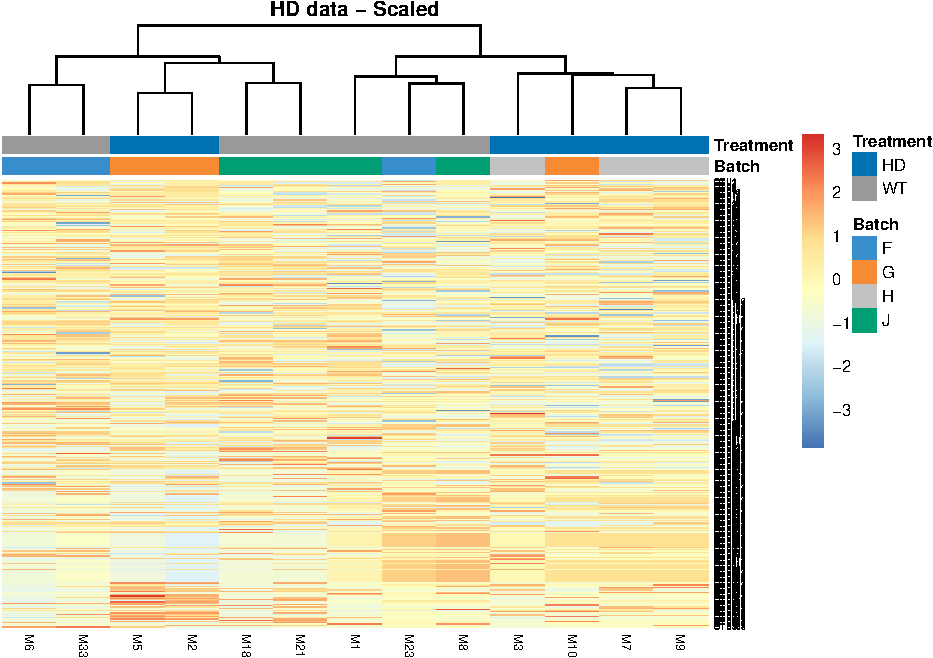
\includegraphics{vignette_files/figure-latex/unnamed-chunk-23-1.pdf}

The batch effect in HD data is not very obviously visualised through
heatmap, because there is no batch with samples clustered together and
separated from other samples.

\chapter{Batch effect adjustment}\label{adjust}

\section{Accounting for batch
effects}\label{accounting-for-batch-effects}

Methods that account for batch effects estimate unknown batch effects
through matrix decomposition and / or assign a known or estimated batch
as a covariate with linear models.

\subsection{Linear model and linear mixed
model}\label{linear-model-and-linear-mixed-model}

LM and LMM are suitable for known batch effects, and can consider batch
x treatment interaction and deal with unbalanced batch x treatment
design. But they are univariate and rely on a Gaussian likelihood
assumption, which may not apply to zero-inflated microbiome data despite
CLR transformation.

We fit a linear model for both sponge and AD data.

\begin{Shaded}
\begin{Highlighting}[]
\CommentTok{# Sponge data}
\NormalTok{sponge.trt_p <-}\StringTok{ }\KeywordTok{apply}\NormalTok{(sponge.tss.clr, }\DecValTok{2}\NormalTok{, }\DataTypeTok{FUN =} \ControlFlowTok{function}\NormalTok{(x)\{}
\NormalTok{  res.lm <-}\StringTok{ }\KeywordTok{lm}\NormalTok{(x }\OperatorTok{~}\StringTok{ }\NormalTok{sponge.trt }\OperatorTok{+}\StringTok{ }\NormalTok{sponge.batch)}
\NormalTok{  summary.res =}\StringTok{ }\KeywordTok{summary}\NormalTok{(res.lm)}
\NormalTok{  p =}\StringTok{ }\NormalTok{summary.res}\OperatorTok{$}\NormalTok{coefficients[}\DecValTok{2}\NormalTok{,}\DecValTok{4}\NormalTok{]}
\NormalTok{\})}

\NormalTok{sponge.trt_q =}\StringTok{ }\KeywordTok{p.adjust}\NormalTok{(sponge.trt_p,}\DataTypeTok{method =} \StringTok{'fdr'}\NormalTok{)}

\CommentTok{# AD data}
\NormalTok{ad.trt_p <-}\StringTok{ }\KeywordTok{apply}\NormalTok{(ad.tss.clr, }\DecValTok{2}\NormalTok{, }\DataTypeTok{FUN =} \ControlFlowTok{function}\NormalTok{(x)\{}
\NormalTok{  res.lm <-}\StringTok{ }\KeywordTok{lm}\NormalTok{(x }\OperatorTok{~}\StringTok{ }\NormalTok{ad.trt }\OperatorTok{+}\StringTok{ }\NormalTok{ad.batch)}
\NormalTok{  summary.res =}\StringTok{ }\KeywordTok{summary}\NormalTok{(res.lm)}
\NormalTok{  p =}\StringTok{ }\NormalTok{summary.res}\OperatorTok{$}\NormalTok{coefficients[}\DecValTok{2}\NormalTok{,}\DecValTok{4}\NormalTok{]}
\NormalTok{\})}

\NormalTok{ad.trt_q =}\StringTok{ }\KeywordTok{p.adjust}\NormalTok{(ad.trt_p,}\DataTypeTok{method =} \StringTok{'fdr'}\NormalTok{)}
\end{Highlighting}
\end{Shaded}

As the batch x treatment design of AD data is unbalaced, we fit a linear
mixed model considering batch (cage) as random effects.

\begin{Shaded}
\begin{Highlighting}[]
\CommentTok{# HD data}
\NormalTok{hd.trt_p <-}\StringTok{ }\KeywordTok{apply}\NormalTok{(hd.tss.clr, }\DecValTok{2}\NormalTok{, }\DataTypeTok{FUN =} \ControlFlowTok{function}\NormalTok{(x)\{}
\NormalTok{  res.lmm <-}\StringTok{ }\KeywordTok{lmer}\NormalTok{(x }\OperatorTok{~}\StringTok{ }\NormalTok{hd.trt }\OperatorTok{+}\StringTok{ }\NormalTok{(}\DecValTok{1}\OperatorTok{|}\NormalTok{hd.batch))}
\NormalTok{  summary.res =}\StringTok{ }\KeywordTok{summary}\NormalTok{(res.lmm)}
\NormalTok{  p =}\StringTok{ }\NormalTok{summary.res}\OperatorTok{$}\NormalTok{coefficients[}\DecValTok{2}\NormalTok{,}\DecValTok{5}\NormalTok{]}
\NormalTok{\})}

\NormalTok{hd.trt_q =}\StringTok{ }\KeywordTok{p.adjust}\NormalTok{(hd.trt_p,}\DataTypeTok{method =} \StringTok{'fdr'}\NormalTok{)}
\end{Highlighting}
\end{Shaded}

\subsection{SVA}\label{sva}

SVA can account for unknown batch effects. But it is univariate, relies
on a Gaussian likelihood assumption and implicitly introduces a
correlation between treatment and batch.

The \emph{sva} function performs two different steps. First it
identifies the number of latent factors that need to be estimated. The
number of factors can be estimated using the \emph{num.sv}.

\begin{Shaded}
\begin{Highlighting}[]
\CommentTok{# sponge data}
\NormalTok{sponge.mod =}\StringTok{ }\KeywordTok{model.matrix}\NormalTok{(}\OperatorTok{~}\NormalTok{sponge.trt) }\CommentTok{# full model}
\NormalTok{sponge.mod0 =}\StringTok{ }\KeywordTok{model.matrix}\NormalTok{(}\OperatorTok{~}\DecValTok{1}\NormalTok{,}\DataTypeTok{data =}\NormalTok{ sponge.trt) }\CommentTok{# null model}
\NormalTok{sponge.sva.n <-}\StringTok{ }\KeywordTok{num.sv}\NormalTok{(}\DataTypeTok{dat =} \KeywordTok{t}\NormalTok{(sponge.tss.clr), }\DataTypeTok{mod =}\NormalTok{ sponge.mod)}
\end{Highlighting}
\end{Shaded}

Next we apply the \emph{sva} function to estimate the surrogate
variables:

\begin{Shaded}
\begin{Highlighting}[]
\NormalTok{sponge.sva =}\StringTok{ }\KeywordTok{sva}\NormalTok{(}\KeywordTok{t}\NormalTok{(sponge.tss.clr), sponge.mod, sponge.mod0, }\DataTypeTok{n.sv =}\NormalTok{ sponge.sva.n)}
\end{Highlighting}
\end{Shaded}

\begin{verbatim}
## Number of significant surrogate variables is:  1 
## Iteration (out of 5 ):1  2  3  4  5
\end{verbatim}

We include the estimated surrogate variables in both the null and full
models. The reason is that we want to adjust for the surrogate
variables, so we treat them as adjustment variables that must be
included in both models. The \emph{f.pvalue} function is then used to
calculate parametric F-test P-values and Q-values (adjusted P-values)
for each OTU of sponge data.

\begin{Shaded}
\begin{Highlighting}[]
\NormalTok{sponge.mod.bat =}\StringTok{ }\KeywordTok{cbind}\NormalTok{(sponge.mod,sponge.sva}\OperatorTok{$}\NormalTok{sv)}
\NormalTok{sponge.mod0.bat =}\StringTok{ }\KeywordTok{cbind}\NormalTok{(sponge.mod0,sponge.sva}\OperatorTok{$}\NormalTok{sv)}

\NormalTok{sponge.sva.trt_p =}\StringTok{ }\KeywordTok{f.pvalue}\NormalTok{(}\KeywordTok{t}\NormalTok{(sponge.tss.clr),sponge.mod.bat,sponge.mod0.bat)}
\NormalTok{sponge.sva.trt_q =}\StringTok{ }\KeywordTok{p.adjust}\NormalTok{(sponge.sva.trt_p,}\DataTypeTok{method=}\StringTok{"fdr"}\NormalTok{)}
\end{Highlighting}
\end{Shaded}

Now these P-values and Q-values are accounting for surrogate variables
(estimated batch effects).

We also apply SVA on both AD and HD data.

\begin{Shaded}
\begin{Highlighting}[]
\CommentTok{# ad data}
\NormalTok{ad.mod =}\StringTok{ }\KeywordTok{model.matrix}\NormalTok{(}\OperatorTok{~}\NormalTok{ad.trt)}
\NormalTok{ad.mod0 =}\StringTok{ }\KeywordTok{model.matrix}\NormalTok{(}\OperatorTok{~}\DecValTok{1}\NormalTok{,}\DataTypeTok{data =}\NormalTok{ ad.trt)}
\NormalTok{ad.sva.n <-}\StringTok{ }\KeywordTok{num.sv}\NormalTok{(}\DataTypeTok{dat =} \KeywordTok{t}\NormalTok{(ad.tss.clr), }\DataTypeTok{mod =}\NormalTok{ ad.mod)}
\NormalTok{ad.sva =}\StringTok{ }\KeywordTok{sva}\NormalTok{(}\KeywordTok{t}\NormalTok{(ad.tss.clr), ad.mod, ad.mod0, }\DataTypeTok{n.sv =}\NormalTok{ ad.sva.n)}
\end{Highlighting}
\end{Shaded}

\begin{verbatim}
## Number of significant surrogate variables is:  6 
## Iteration (out of 5 ):1  2  3  4  5
\end{verbatim}

\begin{Shaded}
\begin{Highlighting}[]
\NormalTok{ad.mod.bat =}\StringTok{ }\KeywordTok{cbind}\NormalTok{(ad.mod,ad.sva}\OperatorTok{$}\NormalTok{sv)}
\NormalTok{ad.mod0.bat =}\StringTok{ }\KeywordTok{cbind}\NormalTok{(ad.mod0,ad.sva}\OperatorTok{$}\NormalTok{sv)}
\NormalTok{ad.sva.trt_p =}\StringTok{ }\KeywordTok{f.pvalue}\NormalTok{(}\KeywordTok{t}\NormalTok{(ad.tss.clr),ad.mod.bat,ad.mod0.bat)}
\NormalTok{ad.sva.trt_q =}\StringTok{ }\KeywordTok{p.adjust}\NormalTok{(ad.sva.trt_p,}\DataTypeTok{method=}\StringTok{"fdr"}\NormalTok{)}

\CommentTok{# hd data}
\NormalTok{hd.mod =}\StringTok{ }\KeywordTok{model.matrix}\NormalTok{(}\OperatorTok{~}\NormalTok{hd.trt)}
\NormalTok{hd.mod0 =}\StringTok{ }\KeywordTok{model.matrix}\NormalTok{(}\OperatorTok{~}\DecValTok{1}\NormalTok{,}\DataTypeTok{data =}\NormalTok{ hd.trt)}
\NormalTok{hd.sva.n <-}\StringTok{ }\KeywordTok{num.sv}\NormalTok{(}\DataTypeTok{dat =} \KeywordTok{t}\NormalTok{(hd.tss.clr), }\DataTypeTok{mod =}\NormalTok{ hd.mod)}
\NormalTok{hd.sva =}\StringTok{ }\KeywordTok{sva}\NormalTok{(}\KeywordTok{t}\NormalTok{(hd.tss.clr), hd.mod, hd.mod0, }\DataTypeTok{n.sv =}\NormalTok{ hd.sva.n)}
\end{Highlighting}
\end{Shaded}

\begin{verbatim}
## Number of significant surrogate variables is:  3 
## Iteration (out of 5 ):1  2  3  4  5
\end{verbatim}

\begin{Shaded}
\begin{Highlighting}[]
\NormalTok{hd.mod.bat =}\StringTok{ }\KeywordTok{cbind}\NormalTok{(hd.mod,hd.sva}\OperatorTok{$}\NormalTok{sv)}
\NormalTok{hd.mod0.bat =}\StringTok{ }\KeywordTok{cbind}\NormalTok{(hd.mod0,hd.sva}\OperatorTok{$}\NormalTok{sv)}
\NormalTok{hd.sva.trt_p =}\StringTok{ }\KeywordTok{f.pvalue}\NormalTok{(}\KeywordTok{t}\NormalTok{(hd.tss.clr),hd.mod.bat,hd.mod0.bat)}
\NormalTok{hd.sva.trt_q =}\StringTok{ }\KeywordTok{p.adjust}\NormalTok{(hd.sva.trt_p,}\DataTypeTok{method=}\StringTok{"fdr"}\NormalTok{)}
\end{Highlighting}
\end{Shaded}

\subsection{RUV2}\label{ruv2}

RUV2 estimates and accounts for unknown batch effects. But it needs
negative control variables that are affected by batch effects but not
treatment effects.

In the real world, we design negative control variables that are not
affected by treatment effects only, we are not sure but assume these
controls are affected by batch effects. RUV2 can only account for the
difference captured by these controls.

Since our three datasets do not have negative control variables, we use
a linear model (or linear mixed model) to identify OTUs less likely to
be affected by treatment effects as negative controls.

\begin{Shaded}
\begin{Highlighting}[]
\CommentTok{# sponge data}
\NormalTok{sponge.nc =}\StringTok{ }\NormalTok{sponge.trt_q }\OperatorTok{>}\StringTok{ }\FloatTok{0.05}
\NormalTok{sponge.ruv2 <-}\StringTok{ }\KeywordTok{RUV2}\NormalTok{(}\DataTypeTok{Y =}\NormalTok{ sponge.tss.clr, }\DataTypeTok{X =}\NormalTok{ sponge.trt, }\DataTypeTok{ctl =}\NormalTok{ sponge.nc, }\DataTypeTok{k =} \DecValTok{3}\NormalTok{) }\CommentTok{# k is subjective}
\NormalTok{sponge.ruv2.trt_p <-}\StringTok{ }\NormalTok{sponge.ruv2}\OperatorTok{$}\NormalTok{p}
\NormalTok{sponge.ruv2.trt_q <-}\StringTok{ }\KeywordTok{p.adjust}\NormalTok{(sponge.ruv2.trt_p,}\DataTypeTok{method=}\StringTok{"fdr"}\NormalTok{)}

\CommentTok{# AD data}
\NormalTok{ad.nc =}\StringTok{ }\NormalTok{ad.trt_q }\OperatorTok{>}\StringTok{ }\FloatTok{0.05}
\NormalTok{ad.ruv2 <-}\StringTok{ }\KeywordTok{RUV2}\NormalTok{(}\DataTypeTok{Y =}\NormalTok{ ad.tss.clr, }\DataTypeTok{X =}\NormalTok{ ad.trt, }\DataTypeTok{ctl =}\NormalTok{ ad.nc, }\DataTypeTok{k =} \DecValTok{3}\NormalTok{) }\CommentTok{# k is subjective}
\NormalTok{ad.ruv2.trt_p <-}\StringTok{ }\NormalTok{ad.ruv2}\OperatorTok{$}\NormalTok{p}
\NormalTok{ad.ruv2.trt_q <-}\StringTok{ }\KeywordTok{p.adjust}\NormalTok{(ad.ruv2.trt_p,}\DataTypeTok{method=}\StringTok{"fdr"}\NormalTok{)}

\CommentTok{# HD data}
\NormalTok{hd.nc =}\StringTok{ }\NormalTok{hd.trt_p }\OperatorTok{>}\StringTok{ }\FloatTok{0.05}
\NormalTok{hd.ruv2 <-}\StringTok{ }\KeywordTok{RUV2}\NormalTok{(}\DataTypeTok{Y =}\NormalTok{ hd.tss.clr, }\DataTypeTok{X =}\NormalTok{ hd.trt, }\DataTypeTok{ctl =}\NormalTok{ hd.nc, }\DataTypeTok{k =} \DecValTok{3}\NormalTok{) }\CommentTok{# k is subjective}
\NormalTok{hd.ruv2.trt_p <-}\StringTok{ }\NormalTok{hd.ruv2}\OperatorTok{$}\NormalTok{p}
\NormalTok{hd.ruv2.trt_q <-}\StringTok{ }\KeywordTok{p.adjust}\NormalTok{(hd.ruv2.trt_p,}\DataTypeTok{method=}\StringTok{"fdr"}\NormalTok{)}
\end{Highlighting}
\end{Shaded}

\subsection{RUV4}\label{ruv4}

\begin{Shaded}
\begin{Highlighting}[]
\CommentTok{# sponge data}
\NormalTok{sponge.k.obj =}\StringTok{ }\KeywordTok{getK}\NormalTok{(}\DataTypeTok{Y =}\NormalTok{ sponge.tss.clr, }\DataTypeTok{X =}\NormalTok{ sponge.trt, }\DataTypeTok{ctl =}\NormalTok{ sponge.nc)}
\NormalTok{sponge.k =}\StringTok{ }\NormalTok{sponge.k.obj}\OperatorTok{$}\NormalTok{k}
\NormalTok{sponge.k =}\StringTok{ }\KeywordTok{ifelse}\NormalTok{(sponge.k }\OperatorTok{!=}\DecValTok{0}\NormalTok{, sponge.k, }\DecValTok{1}\NormalTok{)}
\NormalTok{sponge.ruv4 <-}\StringTok{ }\KeywordTok{RUV4}\NormalTok{(}\DataTypeTok{Y =}\NormalTok{ sponge.tss.clr, }\DataTypeTok{X =}\NormalTok{ sponge.trt, }\DataTypeTok{ctl =}\NormalTok{ sponge.nc, }\DataTypeTok{k =}\NormalTok{ sponge.k) }
\NormalTok{sponge.ruv4.trt_p <-}\StringTok{ }\NormalTok{sponge.ruv4}\OperatorTok{$}\NormalTok{p}
\NormalTok{sponge.ruv4.trt_q <-}\StringTok{ }\KeywordTok{p.adjust}\NormalTok{(sponge.ruv4.trt_p,}\DataTypeTok{method=}\StringTok{"fdr"}\NormalTok{)}

\CommentTok{# AD data}
\NormalTok{ad.k.obj =}\StringTok{ }\KeywordTok{getK}\NormalTok{(}\DataTypeTok{Y =}\NormalTok{ ad.tss.clr, }\DataTypeTok{X =}\NormalTok{ ad.trt, }\DataTypeTok{ctl =}\NormalTok{ ad.nc)}
\NormalTok{ad.k =ad.k.obj}\OperatorTok{$}\NormalTok{k}
\NormalTok{ad.k =}\StringTok{ }\KeywordTok{ifelse}\NormalTok{(ad.k }\OperatorTok{!=}\DecValTok{0}\NormalTok{, ad.k, }\DecValTok{1}\NormalTok{)}
\NormalTok{ad.ruv4 <-}\StringTok{ }\KeywordTok{RUV4}\NormalTok{(}\DataTypeTok{Y =}\NormalTok{ ad.tss.clr, }\DataTypeTok{X =}\NormalTok{ ad.trt, }\DataTypeTok{ctl =}\NormalTok{ ad.nc, }\DataTypeTok{k =}\NormalTok{ ad.k) }
\NormalTok{ad.ruv4.trt_p <-}\StringTok{ }\NormalTok{ad.ruv4}\OperatorTok{$}\NormalTok{p}
\NormalTok{ad.ruv4.trt_q <-}\StringTok{ }\KeywordTok{p.adjust}\NormalTok{(ad.ruv4.trt_p,}\DataTypeTok{method=}\StringTok{"fdr"}\NormalTok{)}

\CommentTok{# HD data}
\NormalTok{hd.k.obj =}\StringTok{ }\KeywordTok{getK}\NormalTok{(}\DataTypeTok{Y =}\NormalTok{ hd.tss.clr, }\DataTypeTok{X =}\NormalTok{ hd.trt, }\DataTypeTok{ctl =}\NormalTok{ hd.nc)}
\NormalTok{hd.k =}\StringTok{ }\NormalTok{hd.k.obj}\OperatorTok{$}\NormalTok{k}
\NormalTok{hd.k =}\StringTok{ }\KeywordTok{ifelse}\NormalTok{(hd.k }\OperatorTok{!=}\DecValTok{0}\NormalTok{, hd.k, }\DecValTok{1}\NormalTok{)}
\NormalTok{hd.ruv4 <-}\StringTok{ }\KeywordTok{RUV4}\NormalTok{(}\DataTypeTok{Y =}\NormalTok{ hd.tss.clr, }\DataTypeTok{X =}\NormalTok{ hd.trt, }\DataTypeTok{ctl =}\NormalTok{ hd.nc, }\DataTypeTok{k =}\NormalTok{ hd.k) }
\NormalTok{hd.ruv4.trt_p <-}\StringTok{ }\NormalTok{hd.ruv4}\OperatorTok{$}\NormalTok{p}
\NormalTok{hd.ruv4.trt_q <-}\StringTok{ }\KeywordTok{p.adjust}\NormalTok{(hd.ruv4.trt_p,}\DataTypeTok{method=}\StringTok{"fdr"}\NormalTok{)}
\end{Highlighting}
\end{Shaded}

\section{Correcting for batch
effects}\label{correcting-for-batch-effects}

\subsection{BMC (batch mean centering)}\label{bmc-batch-mean-centering}

\begin{Shaded}
\begin{Highlighting}[]
\CommentTok{# Sponge data}
\NormalTok{sponge.b1 =}\StringTok{ }\KeywordTok{scale}\NormalTok{(sponge.tss.clr[sponge.batch}\OperatorTok{==}\StringTok{ }\DecValTok{1}\NormalTok{,],}\DataTypeTok{center =} \OtherTok{TRUE}\NormalTok{, }\DataTypeTok{scale =} \OtherTok{FALSE}\NormalTok{)}
\NormalTok{sponge.b2 =}\StringTok{ }\KeywordTok{scale}\NormalTok{(sponge.tss.clr[sponge.batch}\OperatorTok{==}\StringTok{ }\DecValTok{2}\NormalTok{,],}\DataTypeTok{center =} \OtherTok{TRUE}\NormalTok{, }\DataTypeTok{scale =} \OtherTok{FALSE}\NormalTok{)}
\NormalTok{sponge.bmc =}\StringTok{ }\KeywordTok{rbind}\NormalTok{(sponge.b1,sponge.b2)}
\NormalTok{sponge.bmc =}\StringTok{ }\NormalTok{sponge.bmc[}\KeywordTok{rownames}\NormalTok{(sponge.tss.clr),]}

\NormalTok{##############}
\CommentTok{# AD data}
\NormalTok{ad.b1 =}\StringTok{ }\KeywordTok{scale}\NormalTok{(ad.tss.clr[ad.batch}\OperatorTok{==}\StringTok{"09/04/2015"}\NormalTok{,],}\DataTypeTok{center =} \OtherTok{TRUE}\NormalTok{, }\DataTypeTok{scale =} \OtherTok{FALSE}\NormalTok{)}
\NormalTok{ad.b2 =}\StringTok{ }\KeywordTok{scale}\NormalTok{(ad.tss.clr[ad.batch}\OperatorTok{==}\StringTok{"14/04/2016"}\NormalTok{,],}\DataTypeTok{center =} \OtherTok{TRUE}\NormalTok{, }\DataTypeTok{scale =} \OtherTok{FALSE}\NormalTok{)}
\NormalTok{ad.b3 =}\StringTok{ }\KeywordTok{scale}\NormalTok{(ad.tss.clr[ad.batch}\OperatorTok{==}\StringTok{"14/11/2016"}\NormalTok{,],}\DataTypeTok{center =} \OtherTok{TRUE}\NormalTok{, }\DataTypeTok{scale =} \OtherTok{FALSE}\NormalTok{)}
\NormalTok{ad.b4 =}\StringTok{ }\KeywordTok{scale}\NormalTok{(ad.tss.clr[ad.batch}\OperatorTok{==}\StringTok{"01/07/2016"}\NormalTok{,],}\DataTypeTok{center =} \OtherTok{TRUE}\NormalTok{, }\DataTypeTok{scale =} \OtherTok{FALSE}\NormalTok{)}
\NormalTok{ad.b5 =}\StringTok{ }\KeywordTok{scale}\NormalTok{(ad.tss.clr[ad.batch}\OperatorTok{==}\StringTok{"21/09/2017"}\NormalTok{,],}\DataTypeTok{center =} \OtherTok{TRUE}\NormalTok{, }\DataTypeTok{scale =} \OtherTok{FALSE}\NormalTok{)}
\NormalTok{ad.bmc =}\StringTok{ }\KeywordTok{rbind}\NormalTok{(ad.b1,ad.b2,ad.b3,ad.b4,ad.b5)}
\NormalTok{ad.bmc =}\StringTok{ }\NormalTok{ad.bmc[}\KeywordTok{rownames}\NormalTok{(ad.tss.clr),]}
\end{Highlighting}
\end{Shaded}

\subsection{ComBat}\label{combat}

\begin{Shaded}
\begin{Highlighting}[]
\CommentTok{# Sponge data}
\NormalTok{sponge.combat <-}\StringTok{ }\KeywordTok{t}\NormalTok{(}\KeywordTok{ComBat}\NormalTok{(}\KeywordTok{t}\NormalTok{(sponge.tss.clr),}\DataTypeTok{batch=}\NormalTok{sponge.batch,}\DataTypeTok{mod =}\NormalTok{ sponge.mod,}\DataTypeTok{par.prior=}\NormalTok{F,}\DataTypeTok{prior.plots =}\NormalTok{ F))}
\end{Highlighting}
\end{Shaded}

\begin{verbatim}
## Found2batches
\end{verbatim}

\begin{verbatim}
## Adjusting for1covariate(s) or covariate level(s)
\end{verbatim}

\begin{verbatim}
## Standardizing Data across genes
\end{verbatim}

\begin{verbatim}
## Fitting L/S model and finding priors
\end{verbatim}

\begin{verbatim}
## Finding nonparametric adjustments
\end{verbatim}

\begin{verbatim}
## Adjusting the Data
\end{verbatim}

\begin{Shaded}
\begin{Highlighting}[]
\NormalTok{##############}
\CommentTok{# AD data}
\NormalTok{ad.combat <-}\StringTok{ }\KeywordTok{t}\NormalTok{(}\KeywordTok{ComBat}\NormalTok{(}\KeywordTok{t}\NormalTok{(ad.tss.clr),}\DataTypeTok{batch=}\NormalTok{ad.batch,}\DataTypeTok{mod =}\NormalTok{ ad.mod, }\DataTypeTok{par.prior=}\NormalTok{F,}\DataTypeTok{prior.plots =}\NormalTok{ F))}
\end{Highlighting}
\end{Shaded}

\begin{verbatim}
## Found5batches
\end{verbatim}

\begin{verbatim}
## Adjusting for1covariate(s) or covariate level(s)
\end{verbatim}

\begin{verbatim}
## Standardizing Data across genes
\end{verbatim}

\begin{verbatim}
## Fitting L/S model and finding priors
\end{verbatim}

\begin{verbatim}
## Finding nonparametric adjustments
\end{verbatim}

\begin{verbatim}
## Adjusting the Data
\end{verbatim}

\subsection{removeBatchEffect}\label{removebatcheffect}

\begin{Shaded}
\begin{Highlighting}[]
\CommentTok{# Sponge data}
\NormalTok{sponge.limma <-}\StringTok{ }\KeywordTok{t}\NormalTok{(}\KeywordTok{removeBatchEffect}\NormalTok{(}\KeywordTok{t}\NormalTok{(sponge.tss.clr),}\DataTypeTok{batch =}\NormalTok{ sponge.batch,}\DataTypeTok{design =}\NormalTok{ sponge.mod))}

\NormalTok{#############}
\NormalTok{ad.limma <-}\StringTok{ }\KeywordTok{t}\NormalTok{(}\KeywordTok{removeBatchEffect}\NormalTok{(}\KeywordTok{t}\NormalTok{(ad.tss.clr),}\DataTypeTok{batch =}\NormalTok{ ad.batch,}\DataTypeTok{design =}\NormalTok{ ad.mod))}
\end{Highlighting}
\end{Shaded}

\subsection{FAbatch}\label{fabatch}

FAbatch is unable to converge on both sponge data and AD data. This may
influence the effect of batch correction.

\begin{Shaded}
\begin{Highlighting}[]
\CommentTok{# sponge data}
\NormalTok{sponge.fabatch.obj =}\StringTok{ }\KeywordTok{fabatch}\NormalTok{(}\DataTypeTok{x =}\NormalTok{ sponge.tss.clr,}\DataTypeTok{y =} \KeywordTok{as.factor}\NormalTok{(}\KeywordTok{as.numeric}\NormalTok{(sponge.trt)), }\DataTypeTok{batch =}\NormalTok{ sponge.batch)}
\NormalTok{sponge.fabatch <-}\StringTok{ }\NormalTok{sponge.fabatch.obj}\OperatorTok{$}\NormalTok{xadj}

\CommentTok{# ad data}
\NormalTok{ad.fabatch.obj =}\StringTok{ }\KeywordTok{fabatch}\NormalTok{(}\DataTypeTok{x =}\NormalTok{ ad.tss.clr,}\DataTypeTok{y =} \KeywordTok{as.factor}\NormalTok{(}\KeywordTok{as.numeric}\NormalTok{(ad.trt)), }\DataTypeTok{batch =} \KeywordTok{as.factor}\NormalTok{(}\KeywordTok{as.numeric}\NormalTok{(ad.batch)))}
\NormalTok{ad.fabatch <-}\StringTok{ }\NormalTok{ad.fabatch.obj}\OperatorTok{$}\NormalTok{xadj}
\end{Highlighting}
\end{Shaded}

\subsection{percentile normalisation}\label{percentile-normalisation}

\begin{Shaded}
\begin{Highlighting}[]
\NormalTok{sponge.percentile =}\StringTok{ }\KeywordTok{percentile_norm}\NormalTok{(}\DataTypeTok{data =}\NormalTok{ sponge.tss, }\DataTypeTok{batch =}\NormalTok{ sponge.batch, }\DataTypeTok{trt =}\NormalTok{ sponge.trt)}

\CommentTok{# ad data}
\NormalTok{ad.percentile =}\StringTok{ }\KeywordTok{percentile_norm}\NormalTok{(}\DataTypeTok{data =}\NormalTok{ ad.tss, }\DataTypeTok{batch =}\NormalTok{ ad.batch, }\DataTypeTok{trt =}\NormalTok{ ad.trt)}
\end{Highlighting}
\end{Shaded}

\subsection{SVD-based method}\label{svd-based-method}

\begin{Shaded}
\begin{Highlighting}[]
\NormalTok{#################}
\CommentTok{# sponge data}
\NormalTok{sponge.sd =}\StringTok{ }\KeywordTok{apply}\NormalTok{(sponge.tss.clr,}\DecValTok{2}\NormalTok{,sd)}
\NormalTok{sponge.mean =}\StringTok{ }\KeywordTok{apply}\NormalTok{(sponge.tss.clr,}\DecValTok{2}\NormalTok{,mean)}
\NormalTok{X.sponge =}\StringTok{ }\KeywordTok{scale}\NormalTok{(sponge.tss.clr,}\DataTypeTok{center =}\NormalTok{ T,}\DataTypeTok{scale =}\NormalTok{ T)}

\NormalTok{m.sponge =}\StringTok{ }\KeywordTok{crossprod}\NormalTok{(X.sponge)}
\NormalTok{m.svd.sponge =}\StringTok{ }\KeywordTok{svd}\NormalTok{(m.sponge)}
\KeywordTok{barplot}\NormalTok{(m.svd.sponge}\OperatorTok{$}\NormalTok{d)}
\end{Highlighting}
\end{Shaded}

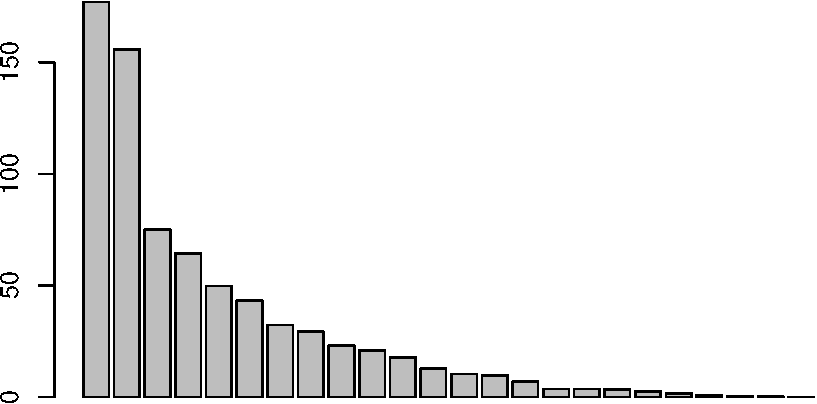
\includegraphics{vignette_files/figure-latex/unnamed-chunk-37-1.pdf}

\begin{Shaded}
\begin{Highlighting}[]
\NormalTok{a1.sponge =}\StringTok{ }\NormalTok{m.svd.sponge}\OperatorTok{$}\NormalTok{u[,}\DecValTok{1}\NormalTok{]}
\NormalTok{b1.sponge =}\StringTok{ }\NormalTok{m.svd.sponge}\OperatorTok{$}\NormalTok{v[,}\DecValTok{1}\NormalTok{]}

\CommentTok{# component 1}
\NormalTok{t1.sponge =}\StringTok{ }\NormalTok{X.sponge }\OperatorTok\StringTok{ }\NormalTok{a1.sponge }\OperatorTok{/}\StringTok{ }\KeywordTok{drop}\NormalTok{(}\KeywordTok{sqrt}\NormalTok{(}\KeywordTok{crossprod}\NormalTok{(a1.sponge)))}
\NormalTok{c1.sponge =}\StringTok{ }\KeywordTok{crossprod}\NormalTok{(X.sponge, t1.sponge) }\OperatorTok{/}\StringTok{ }\KeywordTok{drop}\NormalTok{(}\KeywordTok{crossprod}\NormalTok{(t1.sponge))}
\NormalTok{defl.matrix_svd1.sponge  =}\StringTok{ }\NormalTok{X.sponge }\OperatorTok{-}\StringTok{ }\NormalTok{t1.sponge }\OperatorTok\StringTok{ }\KeywordTok{t}\NormalTok{(c1.sponge)}

\CommentTok{# #}
\NormalTok{sponge.svd =}\StringTok{ }\NormalTok{defl.matrix_svd1.sponge}
\NormalTok{sponge.svd[}\DecValTok{1}\OperatorTok{:}\KeywordTok{nrow}\NormalTok{(sponge.svd),}\DecValTok{1}\OperatorTok{:}\KeywordTok{ncol}\NormalTok{(sponge.svd)] =}\StringTok{ }\OtherTok{NA}
\ControlFlowTok{for}\NormalTok{(i }\ControlFlowTok{in} \DecValTok{1}\OperatorTok{:}\KeywordTok{ncol}\NormalTok{(defl.matrix_svd1.sponge))\{}
  \ControlFlowTok{for}\NormalTok{(j }\ControlFlowTok{in} \DecValTok{1}\OperatorTok{:}\KeywordTok{nrow}\NormalTok{(defl.matrix_svd1.sponge))\{}
\NormalTok{    sponge.svd[j,i] =}\StringTok{ }\NormalTok{defl.matrix_svd1.sponge[j,i]}\OperatorTok{*}\NormalTok{sponge.sd[i] }\OperatorTok{+}\StringTok{ }\NormalTok{sponge.mean[i]}
\NormalTok{  \}}
\NormalTok{\}}

\NormalTok{#####################}
\CommentTok{# ad data}
\NormalTok{ad.sd =}\StringTok{ }\KeywordTok{apply}\NormalTok{(ad.tss.clr,}\DecValTok{2}\NormalTok{,sd)}
\NormalTok{ad.mean =}\StringTok{ }\KeywordTok{apply}\NormalTok{(ad.tss.clr,}\DecValTok{2}\NormalTok{,mean)}
\NormalTok{X.ad =}\StringTok{ }\KeywordTok{scale}\NormalTok{(ad.tss.clr,}\DataTypeTok{center =}\NormalTok{ T,}\DataTypeTok{scale =}\NormalTok{ T)}

\NormalTok{m.ad =}\StringTok{ }\KeywordTok{crossprod}\NormalTok{(X.ad)}
\NormalTok{m.svd.ad =}\StringTok{ }\KeywordTok{svd}\NormalTok{(m.ad)}
\KeywordTok{barplot}\NormalTok{(m.svd.ad}\OperatorTok{$}\NormalTok{d)}
\end{Highlighting}
\end{Shaded}

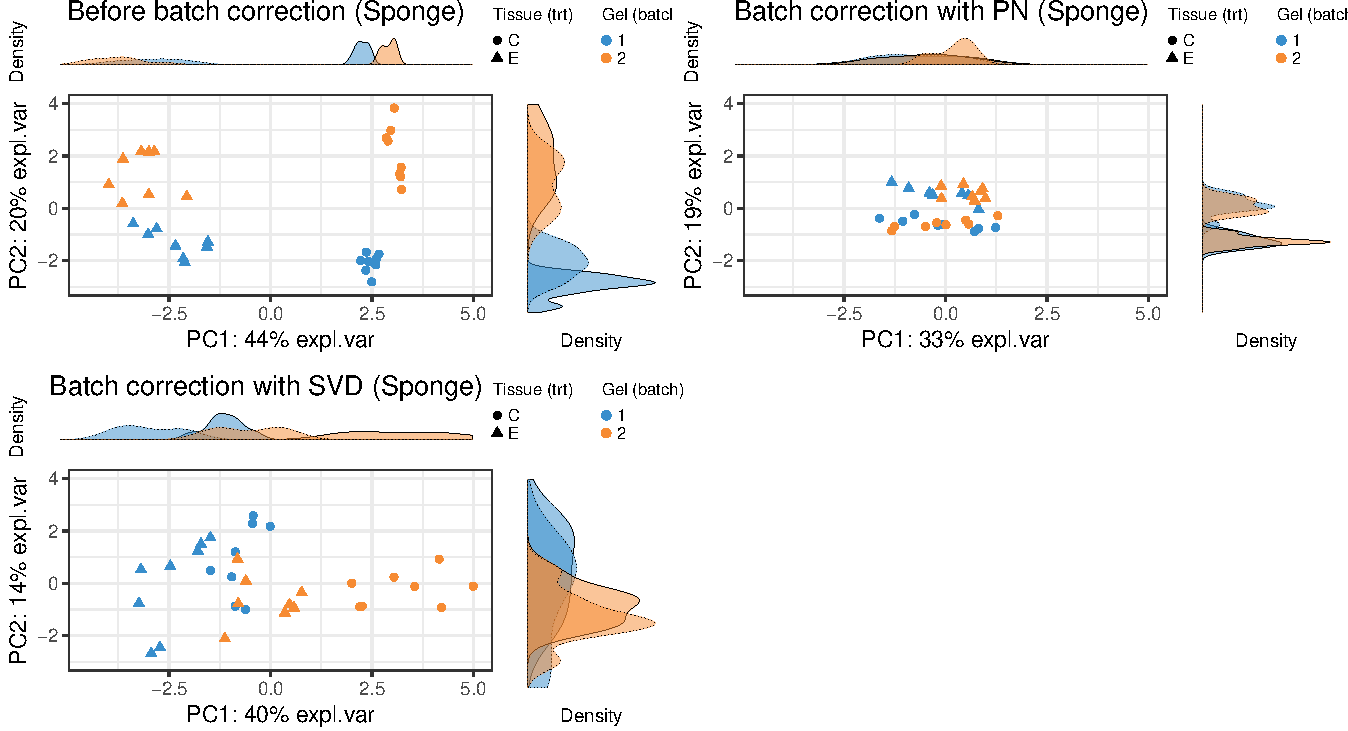
\includegraphics{vignette_files/figure-latex/unnamed-chunk-37-2.pdf}

\begin{Shaded}
\begin{Highlighting}[]
\NormalTok{a1.ad =}\StringTok{ }\NormalTok{m.svd.ad}\OperatorTok{$}\NormalTok{u[,}\DecValTok{1}\NormalTok{]}
\NormalTok{b1.ad =}\StringTok{ }\NormalTok{m.svd.ad}\OperatorTok{$}\NormalTok{v[,}\DecValTok{1}\NormalTok{]}

\CommentTok{# component 1}
\NormalTok{t1.ad =}\StringTok{ }\NormalTok{X.ad }\OperatorTok\StringTok{ }\NormalTok{a1.ad }\OperatorTok{/}\StringTok{ }\KeywordTok{drop}\NormalTok{(}\KeywordTok{sqrt}\NormalTok{(}\KeywordTok{crossprod}\NormalTok{(a1.ad)))}
\NormalTok{c1.ad =}\StringTok{ }\KeywordTok{crossprod}\NormalTok{(X.ad, t1.ad) }\OperatorTok{/}\StringTok{ }\KeywordTok{drop}\NormalTok{(}\KeywordTok{crossprod}\NormalTok{(t1.ad))}
\NormalTok{defl.matrix_svd1.ad  =}\StringTok{ }\NormalTok{X.ad }\OperatorTok{-}\StringTok{ }\NormalTok{t1.ad }\OperatorTok\StringTok{ }\KeywordTok{t}\NormalTok{(c1.ad)}

\CommentTok{# #}
\NormalTok{ad.svd =}\StringTok{ }\NormalTok{defl.matrix_svd1.ad}
\NormalTok{ad.svd[}\DecValTok{1}\OperatorTok{:}\KeywordTok{nrow}\NormalTok{(ad.svd),}\DecValTok{1}\OperatorTok{:}\KeywordTok{ncol}\NormalTok{(ad.svd)] =}\StringTok{ }\OtherTok{NA}
\ControlFlowTok{for}\NormalTok{(i }\ControlFlowTok{in} \DecValTok{1}\OperatorTok{:}\KeywordTok{ncol}\NormalTok{(defl.matrix_svd1.ad))\{}
  \ControlFlowTok{for}\NormalTok{(j }\ControlFlowTok{in} \DecValTok{1}\OperatorTok{:}\KeywordTok{nrow}\NormalTok{(defl.matrix_svd1.ad))\{}
\NormalTok{    ad.svd[j,i] =}\StringTok{ }\NormalTok{defl.matrix_svd1.ad[j,i]}\OperatorTok{*}\NormalTok{ad.sd[i] }\OperatorTok{+}\StringTok{ }\NormalTok{ad.mean[i]}
\NormalTok{  \}}
\NormalTok{\}}
\end{Highlighting}
\end{Shaded}

\subsection{RUVIII}\label{ruviii}

RUVIII needs technical sample replicates and negative control variables.
As only AD data have sample replicates, RUVIII is only applied on AD
data. We use linear model to find variables with less probability of
treatment effects, and these variables are treated as negative control
variables to fit the assumptions of RUVIII.

\begin{Shaded}
\begin{Highlighting}[]
\NormalTok{#####################}
\CommentTok{# ad data only}
\NormalTok{replicates.ad =}\StringTok{ }\NormalTok{ad.metadata}\OperatorTok{$}\NormalTok{sample_name.data.extraction}
\NormalTok{replicates.ad.matrix =}\StringTok{ }\KeywordTok{replicate.matrix}\NormalTok{(replicates.ad)}

\NormalTok{p.ad =}\StringTok{ }\KeywordTok{matrix}\NormalTok{(}\OtherTok{NA}\NormalTok{,}\DataTypeTok{nrow =} \DecValTok{2}\NormalTok{, }\DataTypeTok{ncol =} \KeywordTok{ncol}\NormalTok{(ad.tss.clr))}
\KeywordTok{rownames}\NormalTok{(p.ad) =}\StringTok{ }\KeywordTok{c}\NormalTok{(}\StringTok{'ad.trt'}\NormalTok{,}\StringTok{'ad.batch'}\NormalTok{)}
\KeywordTok{colnames}\NormalTok{(p.ad) =}\StringTok{ }\KeywordTok{colnames}\NormalTok{(ad.tss.clr)}
\ControlFlowTok{for}\NormalTok{(i }\ControlFlowTok{in} \DecValTok{1}\OperatorTok{:}\KeywordTok{ncol}\NormalTok{(ad.tss.clr))\{}
\NormalTok{  res =}\StringTok{ }\KeywordTok{lm}\NormalTok{(ad.tss.clr[,i] }\OperatorTok{~}\StringTok{ }\NormalTok{ad.trt }\OperatorTok{+}\StringTok{ }\NormalTok{ad.batch)}
\NormalTok{  summ.res =}\StringTok{ }\KeywordTok{summary}\NormalTok{(res)}
\NormalTok{  anova.res =}\StringTok{ }\KeywordTok{anova}\NormalTok{(res)}
\NormalTok{  p.ad[}\DecValTok{1}\NormalTok{,i] =}\StringTok{ }\NormalTok{anova.res}\OperatorTok{$}\StringTok{`}\DataTypeTok{Pr(>F)}\StringTok{`}\NormalTok{[}\DecValTok{1}\NormalTok{]}
\NormalTok{  p.ad[}\DecValTok{2}\NormalTok{,i] =}\StringTok{ }\NormalTok{anova.res}\OperatorTok{$}\StringTok{`}\DataTypeTok{Pr(>F)}\StringTok{`}\NormalTok{[}\DecValTok{2}\NormalTok{]}
\NormalTok{\}}

\NormalTok{p.adj.ad =}\StringTok{ }\KeywordTok{apply}\NormalTok{(p.ad,}\DecValTok{1}\NormalTok{,p.adjust,}\DataTypeTok{method =} \StringTok{'fdr'}\NormalTok{)}
\NormalTok{p.adj.ad1 =}\StringTok{ }\KeywordTok{sort}\NormalTok{(p.adj.ad[,}\DecValTok{1}\NormalTok{],}\DataTypeTok{decreasing =}\NormalTok{ T)}
\NormalTok{nc.otu1 =}\StringTok{ }\KeywordTok{names}\NormalTok{(p.adj.ad1[}\DecValTok{1}\OperatorTok{:}\DecValTok{75}\NormalTok{]) }\CommentTok{#negative control genes need be equal or more than samples}
\NormalTok{nc1 =}\StringTok{ }\KeywordTok{rep}\NormalTok{(}\OtherTok{FALSE}\NormalTok{, }\KeywordTok{ncol}\NormalTok{(ad.tss.clr))}
\KeywordTok{names}\NormalTok{(nc1) =}\StringTok{ }\KeywordTok{colnames}\NormalTok{(ad.tss.clr)}
\NormalTok{nc1[nc.otu1] =}\StringTok{ }\OtherTok{TRUE}

\NormalTok{ad.ruv <-}\StringTok{ }\KeywordTok{RUVIII}\NormalTok{(}\DataTypeTok{Y=}\NormalTok{ad.tss.clr,}\DataTypeTok{M =}\NormalTok{ replicates.ad.matrix, }\DataTypeTok{ctl =}\NormalTok{ nc1)}
\KeywordTok{rownames}\NormalTok{(ad.ruv) =}\StringTok{ }\KeywordTok{rownames}\NormalTok{(ad.tss.clr)}
\end{Highlighting}
\end{Shaded}

\chapter{Methods evaluation}\label{eval}

\section{Diagnostic plots}\label{diagnostic-plots}

\subsection{Principal component analysis (PCA) with density plot per
component}\label{principal-component-analysis-pca-with-density-plot-per-component-1}

\begin{Shaded}
\begin{Highlighting}[]
\CommentTok{# sponge data}
\NormalTok{pca.sponge.before =}\StringTok{ }\KeywordTok{pca}\NormalTok{(sponge.tss.clr, }\DataTypeTok{ncomp =} \DecValTok{3}\NormalTok{)}
\NormalTok{pca.sponge.bmc =}\StringTok{ }\KeywordTok{pca}\NormalTok{(sponge.bmc, }\DataTypeTok{ncomp =} \DecValTok{3}\NormalTok{)}
\NormalTok{pca.sponge.combat =}\StringTok{ }\KeywordTok{pca}\NormalTok{(sponge.combat, }\DataTypeTok{ncomp =} \DecValTok{3}\NormalTok{)}
\NormalTok{pca.sponge.limma =}\StringTok{ }\KeywordTok{pca}\NormalTok{(sponge.limma, }\DataTypeTok{ncomp =} \DecValTok{3}\NormalTok{)}
\NormalTok{pca.sponge.percentile =}\StringTok{ }\KeywordTok{pca}\NormalTok{(sponge.percentile, }\DataTypeTok{ncomp =} \DecValTok{3}\NormalTok{)}
\NormalTok{pca.sponge.svd =}\StringTok{ }\KeywordTok{pca}\NormalTok{(sponge.svd, }\DataTypeTok{ncomp =} \DecValTok{3}\NormalTok{)}

\CommentTok{# ad data}
\NormalTok{pca.ad.before =}\StringTok{ }\KeywordTok{pca}\NormalTok{(ad.tss.clr, }\DataTypeTok{ncomp =} \DecValTok{3}\NormalTok{)}
\NormalTok{pca.ad.bmc =}\StringTok{ }\KeywordTok{pca}\NormalTok{(ad.bmc, }\DataTypeTok{ncomp =} \DecValTok{3}\NormalTok{)}
\NormalTok{pca.ad.combat =}\StringTok{ }\KeywordTok{pca}\NormalTok{(ad.combat, }\DataTypeTok{ncomp =} \DecValTok{3}\NormalTok{)}
\NormalTok{pca.ad.limma =}\StringTok{ }\KeywordTok{pca}\NormalTok{(ad.limma, }\DataTypeTok{ncomp =} \DecValTok{3}\NormalTok{)}
\NormalTok{pca.ad.percentile =}\StringTok{ }\KeywordTok{pca}\NormalTok{(ad.percentile, }\DataTypeTok{ncomp =} \DecValTok{3}\NormalTok{)}
\NormalTok{pca.ad.svd =}\StringTok{ }\KeywordTok{pca}\NormalTok{(ad.svd, }\DataTypeTok{ncomp =} \DecValTok{3}\NormalTok{)}
\NormalTok{pca.ad.ruv =}\StringTok{ }\KeywordTok{pca}\NormalTok{(ad.ruv, }\DataTypeTok{ncomp =} \DecValTok{3}\NormalTok{)}
\end{Highlighting}
\end{Shaded}

\begin{Shaded}
\begin{Highlighting}[]
\KeywordTok{grid.arrange}\NormalTok{(plot.pca.before.sponge, plot.pca.bmc.sponge, plot.pca.combat.sponge,plot.pca.limma.sponge,}\DataTypeTok{ncol=}\DecValTok{2}\NormalTok{)}
\end{Highlighting}
\end{Shaded}

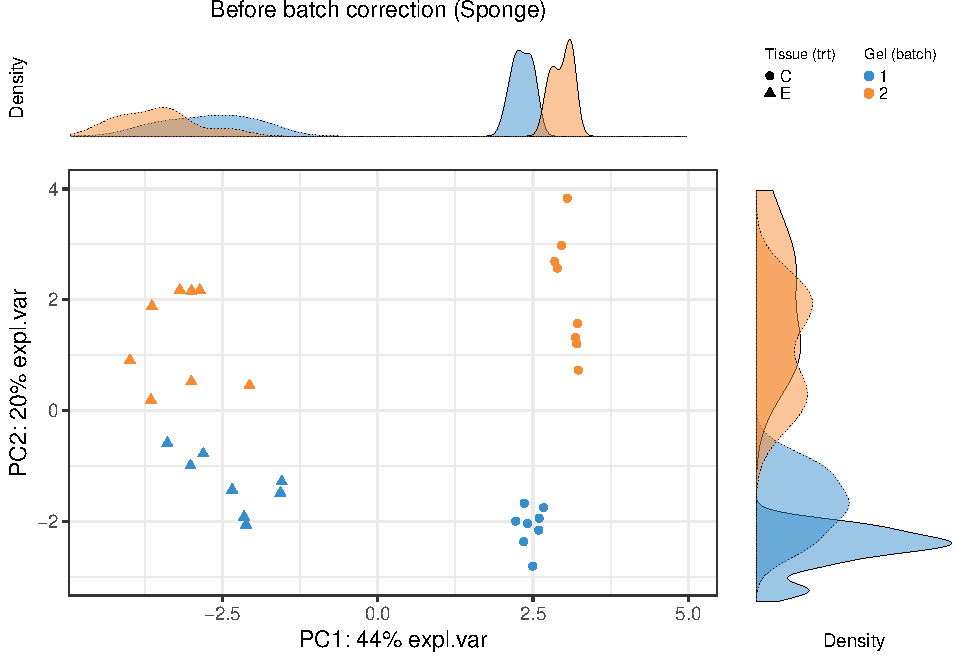
\includegraphics{vignette_files/figure-latex/unnamed-chunk-41-1.pdf}

\begin{Shaded}
\begin{Highlighting}[]
\KeywordTok{grid.arrange}\NormalTok{(plot.pca.before.sponge, plot.pca.percentile.sponge,plot.pca.svd.sponge,}\DataTypeTok{ncol=}\DecValTok{2}\NormalTok{)}
\end{Highlighting}
\end{Shaded}

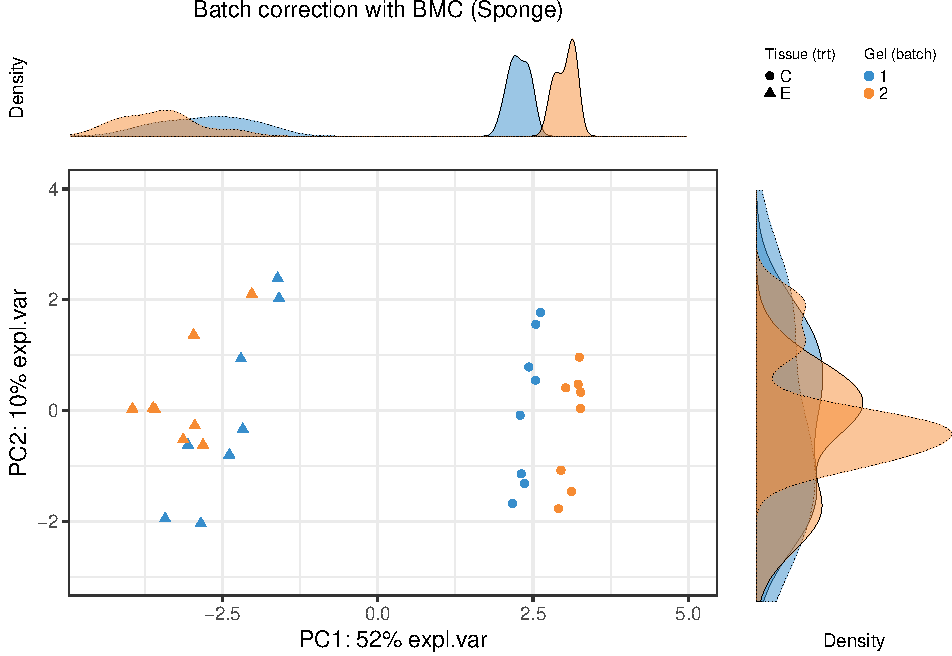
\includegraphics{vignette_files/figure-latex/unnamed-chunk-41-2.pdf}

\begin{Shaded}
\begin{Highlighting}[]
\KeywordTok{grid.arrange}\NormalTok{(plot.pca.before.ad, plot.pca.bmc.ad, plot.pca.combat.ad,plot.pca.limma.ad,}\DataTypeTok{ncol=}\DecValTok{2}\NormalTok{)}
\end{Highlighting}
\end{Shaded}

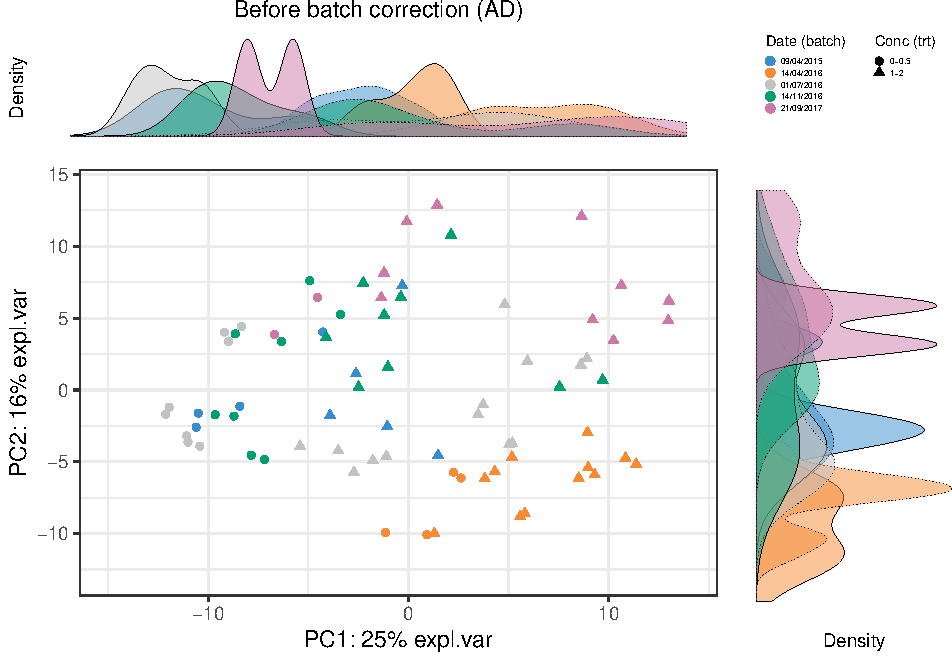
\includegraphics{vignette_files/figure-latex/unnamed-chunk-43-1.pdf}

\begin{Shaded}
\begin{Highlighting}[]
\KeywordTok{grid.arrange}\NormalTok{(plot.pca.before.ad, plot.pca.percentile.ad,plot.pca.svd.ad,plot.pca.ruv.ad,}\DataTypeTok{ncol=}\DecValTok{2}\NormalTok{)}
\end{Highlighting}
\end{Shaded}

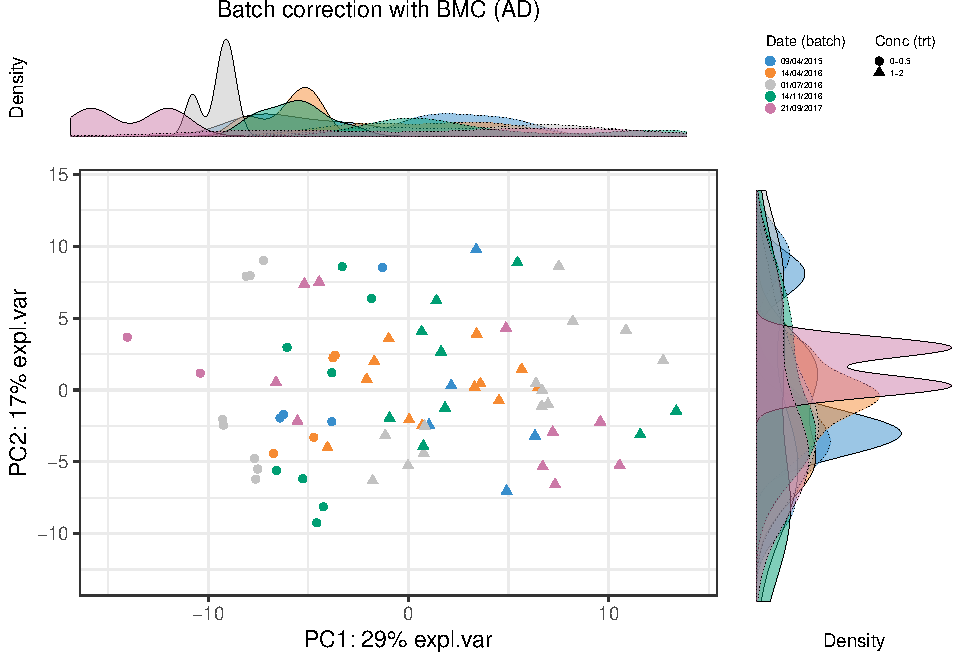
\includegraphics{vignette_files/figure-latex/unnamed-chunk-43-2.pdf}

\subsection{Density plot and box
plot}\label{density-plot-and-box-plot-1}

\begin{Shaded}
\begin{Highlighting}[]
\NormalTok{###############}
\NormalTok{## sponge data}
\NormalTok{sponge.before.df =}\StringTok{ }\KeywordTok{data.frame}\NormalTok{(}\DataTypeTok{value =}\NormalTok{ sponge.tss.clr[,}\DecValTok{9}\NormalTok{], }\DataTypeTok{batch =}\NormalTok{ sponge.batch)}
\NormalTok{sponge.before.boxplot <-}\StringTok{ }\KeywordTok{box_plot_fun}\NormalTok{(}\DataTypeTok{data =}\NormalTok{ sponge.before.df,}\DataTypeTok{x=}\NormalTok{sponge.before.df}\OperatorTok{$}\NormalTok{batch,}
             \DataTypeTok{y=}\NormalTok{sponge.before.df}\OperatorTok{$}\NormalTok{value,}\DataTypeTok{title =} \StringTok{'OTU9 - before (Sponge)'}\NormalTok{,}
             \DataTypeTok{batch.legend.title =} \StringTok{'Gel (batch)'}\NormalTok{)}

\NormalTok{sponge.bmc.df =}\StringTok{ }\KeywordTok{data.frame}\NormalTok{(}\DataTypeTok{value =}\NormalTok{ sponge.bmc[,}\DecValTok{9}\NormalTok{], }\DataTypeTok{batch =}\NormalTok{ sponge.batch)}
\NormalTok{sponge.bmc.boxplot <-}\KeywordTok{box_plot_fun}\NormalTok{(}\DataTypeTok{data =}\NormalTok{ sponge.bmc.df,}\DataTypeTok{x=}\NormalTok{sponge.bmc.df}\OperatorTok{$}\NormalTok{batch,}
             \DataTypeTok{y=}\NormalTok{sponge.bmc.df}\OperatorTok{$}\NormalTok{value,}\DataTypeTok{title =} \StringTok{'OTU9 - BMC (Sponge)'}\NormalTok{,}
             \DataTypeTok{batch.legend.title =} \StringTok{'Gel (batch)'}\NormalTok{)}


\NormalTok{sponge.combat.df =}\StringTok{ }\KeywordTok{data.frame}\NormalTok{(}\DataTypeTok{value =}\NormalTok{ sponge.combat[,}\DecValTok{9}\NormalTok{], }\DataTypeTok{batch =}\NormalTok{ sponge.batch)}
\NormalTok{sponge.combat.boxplot <-}\KeywordTok{box_plot_fun}\NormalTok{(}\DataTypeTok{data =}\NormalTok{ sponge.combat.df,}\DataTypeTok{x=}\NormalTok{sponge.combat.df}\OperatorTok{$}\NormalTok{batch,}
             \DataTypeTok{y=}\NormalTok{sponge.combat.df}\OperatorTok{$}\NormalTok{value,}\DataTypeTok{title =} \StringTok{'OTU9 - ComBat (Sponge)'}\NormalTok{,}
             \DataTypeTok{batch.legend.title =} \StringTok{'Gel (batch)'}\NormalTok{)}


\NormalTok{sponge.limma.df =}\StringTok{ }\KeywordTok{data.frame}\NormalTok{(}\DataTypeTok{value =}\NormalTok{ sponge.limma[,}\DecValTok{9}\NormalTok{], }\DataTypeTok{batch =}\NormalTok{ sponge.batch)}
\NormalTok{sponge.limma.boxplot <-}\KeywordTok{box_plot_fun}\NormalTok{(}\DataTypeTok{data =}\NormalTok{ sponge.limma.df,}\DataTypeTok{x=}\NormalTok{sponge.limma.df}\OperatorTok{$}\NormalTok{batch,}
             \DataTypeTok{y=}\NormalTok{sponge.limma.df}\OperatorTok{$}\NormalTok{value,}\DataTypeTok{title =} \StringTok{'OTU9 - rBE(Sponge)'}\NormalTok{,}
             \DataTypeTok{batch.legend.title =} \StringTok{'Gel (batch)'}\NormalTok{)}

\NormalTok{sponge.percentile.df =}\StringTok{ }\KeywordTok{data.frame}\NormalTok{(}\DataTypeTok{value =}\NormalTok{ sponge.percentile[,}\DecValTok{9}\NormalTok{], }\DataTypeTok{batch =}\NormalTok{ sponge.batch)}
\NormalTok{sponge.percentile.boxplot <-}\KeywordTok{box_plot_fun}\NormalTok{(}\DataTypeTok{data =}\NormalTok{ sponge.percentile.df,}\DataTypeTok{x=}\NormalTok{sponge.percentile.df}\OperatorTok{$}\NormalTok{batch,}
             \DataTypeTok{y=}\NormalTok{sponge.percentile.df}\OperatorTok{$}\NormalTok{value,}\DataTypeTok{title =} \StringTok{'OTU9 - PN (Sponge)'}\NormalTok{,}
             \DataTypeTok{batch.legend.title =} \StringTok{'Gel (batch)'}\NormalTok{)}

\NormalTok{sponge.svd.df =}\StringTok{ }\KeywordTok{data.frame}\NormalTok{(}\DataTypeTok{value =}\NormalTok{ sponge.svd[,}\DecValTok{9}\NormalTok{], }\DataTypeTok{batch =}\NormalTok{ sponge.batch)}
\NormalTok{sponge.svd.boxplot <-}\KeywordTok{box_plot_fun}\NormalTok{(}\DataTypeTok{data =}\NormalTok{ sponge.svd.df,}\DataTypeTok{x=}\NormalTok{sponge.svd.df}\OperatorTok{$}\NormalTok{batch,}
             \DataTypeTok{y=}\NormalTok{sponge.svd.df}\OperatorTok{$}\NormalTok{value,}\DataTypeTok{title =} \StringTok{'OTU9 - SVD (Sponge)'}\NormalTok{,}
             \DataTypeTok{batch.legend.title =} \StringTok{'Gel (batch)'}\NormalTok{)}
\end{Highlighting}
\end{Shaded}

\begin{Shaded}
\begin{Highlighting}[]
\KeywordTok{grid.arrange}\NormalTok{(sponge.before.boxplot, sponge.bmc.boxplot, sponge.combat.boxplot, sponge.limma.boxplot,}\DataTypeTok{ncol=}\DecValTok{2}\NormalTok{)}
\end{Highlighting}
\end{Shaded}

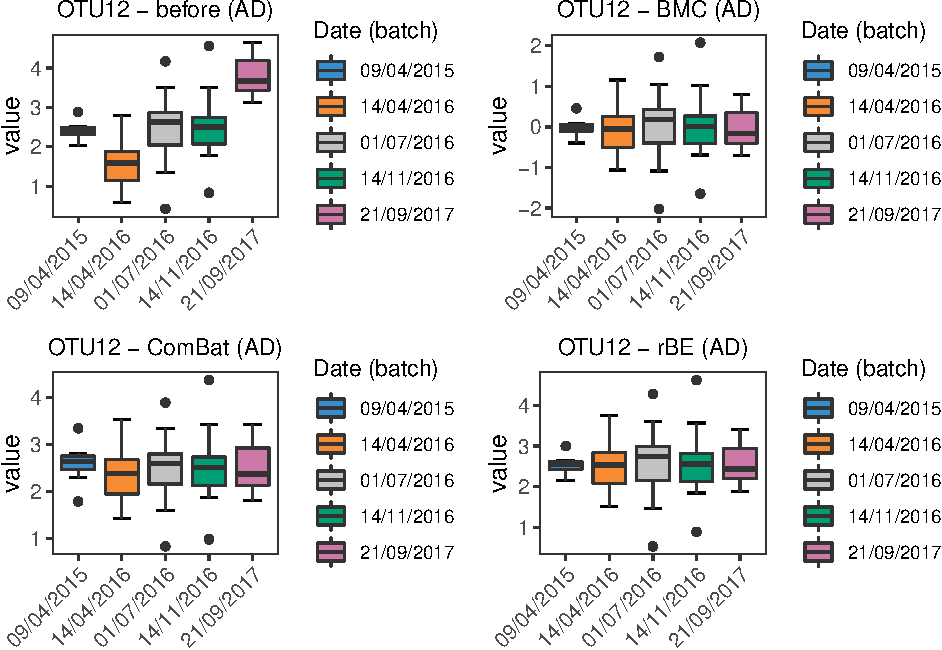
\includegraphics{vignette_files/figure-latex/unnamed-chunk-45-1.pdf}

\begin{Shaded}
\begin{Highlighting}[]
\KeywordTok{grid.arrange}\NormalTok{(sponge.before.boxplot, sponge.percentile.boxplot,sponge.svd.boxplot,}\DataTypeTok{ncol=}\DecValTok{2}\NormalTok{)}
\end{Highlighting}
\end{Shaded}

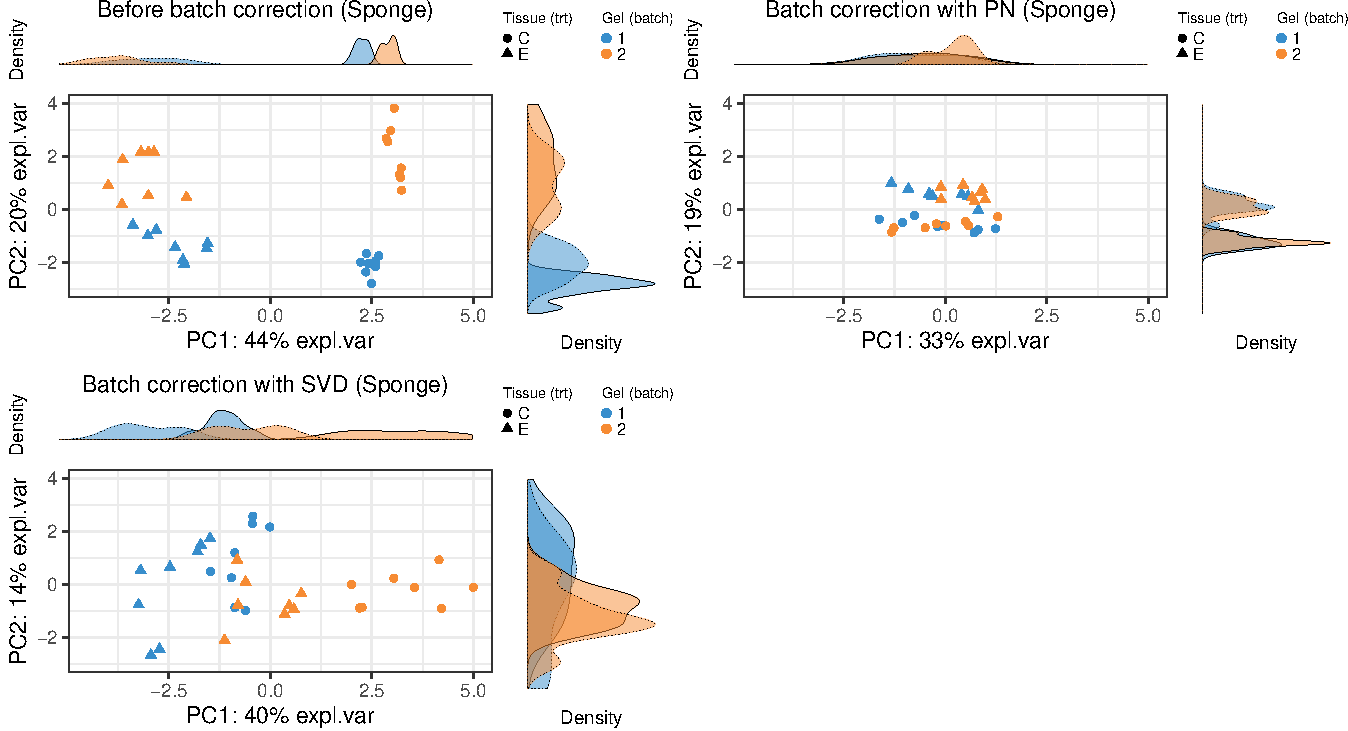
\includegraphics{vignette_files/figure-latex/unnamed-chunk-45-2.pdf}

\begin{Shaded}
\begin{Highlighting}[]
\NormalTok{## density plot}
\CommentTok{# before}
\NormalTok{plot.sponge.before <-}\StringTok{ }\KeywordTok{ggplot}\NormalTok{(sponge.before.df, }\KeywordTok{aes}\NormalTok{(}\DataTypeTok{x =}\NormalTok{ value, }\DataTypeTok{fill =}\NormalTok{ batch)) }\OperatorTok{+}\StringTok{ }\KeywordTok{geom_density}\NormalTok{(}\DataTypeTok{alpha =} \FloatTok{0.5}\NormalTok{) }\OperatorTok{+}\StringTok{ }\KeywordTok{scale_fill_manual}\NormalTok{(}\DataTypeTok{values=}\KeywordTok{color.mixo}\NormalTok{(}\DecValTok{1}\OperatorTok{:}\DecValTok{10}\NormalTok{)) }\OperatorTok{+}\StringTok{ }\KeywordTok{labs}\NormalTok{(}\DataTypeTok{title =} \StringTok{'OTU9 - before (Sponge)'}\NormalTok{,}\DataTypeTok{x=}\StringTok{'Value'}\NormalTok{,}\DataTypeTok{fill =} \StringTok{'Gel (batch)'}\NormalTok{) }\OperatorTok{+}\StringTok{ }\KeywordTok{theme_bw}\NormalTok{() }\OperatorTok{+}\StringTok{ }\KeywordTok{theme}\NormalTok{(}\DataTypeTok{plot.title =} \KeywordTok{element_text}\NormalTok{(}\DataTypeTok{hjust=}\FloatTok{0.5}\NormalTok{), }\DataTypeTok{panel.grid =} \KeywordTok{element_blank}\NormalTok{())}

\CommentTok{# BMC}
\NormalTok{plot.sponge.bmc <-}\StringTok{ }\KeywordTok{ggplot}\NormalTok{(sponge.bmc.df, }\KeywordTok{aes}\NormalTok{(}\DataTypeTok{x =}\NormalTok{ value, }\DataTypeTok{fill =}\NormalTok{ batch)) }\OperatorTok{+}\StringTok{ }\KeywordTok{geom_density}\NormalTok{(}\DataTypeTok{alpha =} \FloatTok{0.5}\NormalTok{) }\OperatorTok{+}\StringTok{ }\KeywordTok{scale_fill_manual}\NormalTok{(}\DataTypeTok{values=}\KeywordTok{color.mixo}\NormalTok{(}\DecValTok{1}\OperatorTok{:}\DecValTok{10}\NormalTok{)) }\OperatorTok{+}\StringTok{ }\KeywordTok{labs}\NormalTok{(}\DataTypeTok{title =} \StringTok{'OTU9 - BMC (Sponge)'}\NormalTok{,}\DataTypeTok{x=}\StringTok{'Value'}\NormalTok{,}\DataTypeTok{fill =} \StringTok{'Gel (batch)'}\NormalTok{) }\OperatorTok{+}\StringTok{ }\KeywordTok{theme_bw}\NormalTok{() }\OperatorTok{+}\StringTok{ }\KeywordTok{theme}\NormalTok{(}\DataTypeTok{plot.title =} \KeywordTok{element_text}\NormalTok{(}\DataTypeTok{hjust=}\FloatTok{0.5}\NormalTok{), }\DataTypeTok{panel.grid =} \KeywordTok{element_blank}\NormalTok{())}


\CommentTok{# ComBat}
\NormalTok{plot.sponge.combat <-}\StringTok{ }\KeywordTok{ggplot}\NormalTok{(sponge.combat.df, }\KeywordTok{aes}\NormalTok{(}\DataTypeTok{x =}\NormalTok{ value, }\DataTypeTok{fill =}\NormalTok{ batch)) }\OperatorTok{+}\StringTok{ }\KeywordTok{geom_density}\NormalTok{(}\DataTypeTok{alpha =} \FloatTok{0.5}\NormalTok{) }\OperatorTok{+}\StringTok{ }\KeywordTok{scale_fill_manual}\NormalTok{(}\DataTypeTok{values=}\KeywordTok{color.mixo}\NormalTok{(}\DecValTok{1}\OperatorTok{:}\DecValTok{10}\NormalTok{)) }\OperatorTok{+}\StringTok{ }\KeywordTok{labs}\NormalTok{(}\DataTypeTok{title =} \StringTok{'OTU9 - ComBat (Sponge)'}\NormalTok{,}\DataTypeTok{x=}\StringTok{'Value'}\NormalTok{,}\DataTypeTok{fill =} \StringTok{'Gel (batch)'}\NormalTok{) }\OperatorTok{+}\StringTok{ }\KeywordTok{theme_bw}\NormalTok{() }\OperatorTok{+}\StringTok{ }\KeywordTok{theme}\NormalTok{(}\DataTypeTok{plot.title =} \KeywordTok{element_text}\NormalTok{(}\DataTypeTok{hjust=}\FloatTok{0.5}\NormalTok{), }\DataTypeTok{panel.grid =} \KeywordTok{element_blank}\NormalTok{())}


\CommentTok{# removeBatchEffect }
\NormalTok{plot.sponge.limma <-}\StringTok{ }\KeywordTok{ggplot}\NormalTok{(sponge.limma.df, }\KeywordTok{aes}\NormalTok{(}\DataTypeTok{x =}\NormalTok{ value, }\DataTypeTok{fill =}\NormalTok{ batch)) }\OperatorTok{+}\StringTok{ }\KeywordTok{geom_density}\NormalTok{(}\DataTypeTok{alpha =} \FloatTok{0.5}\NormalTok{) }\OperatorTok{+}\StringTok{ }\KeywordTok{scale_fill_manual}\NormalTok{(}\DataTypeTok{values=}\KeywordTok{color.mixo}\NormalTok{(}\DecValTok{1}\OperatorTok{:}\DecValTok{10}\NormalTok{)) }\OperatorTok{+}\StringTok{ }\KeywordTok{labs}\NormalTok{(}\DataTypeTok{title =} \StringTok{'OTU9 - rBE (Sponge)'}\NormalTok{,}\DataTypeTok{x=}\StringTok{'Value'}\NormalTok{,}\DataTypeTok{fill =} \StringTok{'Gel (batch)'}\NormalTok{) }\OperatorTok{+}\StringTok{ }\KeywordTok{theme_bw}\NormalTok{() }\OperatorTok{+}\StringTok{ }\KeywordTok{theme}\NormalTok{(}\DataTypeTok{plot.title =} \KeywordTok{element_text}\NormalTok{(}\DataTypeTok{hjust=}\FloatTok{0.5}\NormalTok{), }\DataTypeTok{panel.grid =} \KeywordTok{element_blank}\NormalTok{())}


\CommentTok{# percentile normal}
\NormalTok{plot.sponge.percentile <-}\StringTok{ }\KeywordTok{ggplot}\NormalTok{(sponge.percentile.df, }\KeywordTok{aes}\NormalTok{(}\DataTypeTok{x =}\NormalTok{ value, }\DataTypeTok{fill =}\NormalTok{ batch)) }\OperatorTok{+}\StringTok{ }\KeywordTok{geom_density}\NormalTok{(}\DataTypeTok{alpha =} \FloatTok{0.5}\NormalTok{) }\OperatorTok{+}\StringTok{ }\KeywordTok{scale_fill_manual}\NormalTok{(}\DataTypeTok{values=}\KeywordTok{color.mixo}\NormalTok{(}\DecValTok{1}\OperatorTok{:}\DecValTok{10}\NormalTok{)) }\OperatorTok{+}\StringTok{ }\KeywordTok{labs}\NormalTok{(}\DataTypeTok{title =} \StringTok{'OTU9 - PN (Sponge)'}\NormalTok{,}\DataTypeTok{x=}\StringTok{'Value'}\NormalTok{,}\DataTypeTok{fill =} \StringTok{'Gel (batch)'}\NormalTok{) }\OperatorTok{+}\StringTok{ }\KeywordTok{theme_bw}\NormalTok{() }\OperatorTok{+}\StringTok{ }\KeywordTok{theme}\NormalTok{(}\DataTypeTok{plot.title =} \KeywordTok{element_text}\NormalTok{(}\DataTypeTok{hjust=}\FloatTok{0.5}\NormalTok{), }\DataTypeTok{panel.grid =} \KeywordTok{element_blank}\NormalTok{())}


\CommentTok{# SVD}
\NormalTok{plot.sponge.svd <-}\StringTok{ }\KeywordTok{ggplot}\NormalTok{(sponge.svd.df, }\KeywordTok{aes}\NormalTok{(}\DataTypeTok{x =}\NormalTok{ value, }\DataTypeTok{fill =}\NormalTok{ batch)) }\OperatorTok{+}\StringTok{ }\KeywordTok{geom_density}\NormalTok{(}\DataTypeTok{alpha =} \FloatTok{0.5}\NormalTok{) }\OperatorTok{+}\StringTok{ }\KeywordTok{scale_fill_manual}\NormalTok{(}\DataTypeTok{values=}\KeywordTok{color.mixo}\NormalTok{(}\DecValTok{1}\OperatorTok{:}\DecValTok{10}\NormalTok{)) }\OperatorTok{+}\StringTok{ }\KeywordTok{labs}\NormalTok{(}\DataTypeTok{title =} \StringTok{'OTU9 - SVD (Sponge)'}\NormalTok{,}\DataTypeTok{x=}\StringTok{'Value'}\NormalTok{,}\DataTypeTok{fill =} \StringTok{'Gel (batch)'}\NormalTok{) }\OperatorTok{+}\StringTok{ }\KeywordTok{theme_bw}\NormalTok{() }\OperatorTok{+}\StringTok{ }\KeywordTok{theme}\NormalTok{(}\DataTypeTok{plot.title =} \KeywordTok{element_text}\NormalTok{(}\DataTypeTok{hjust=}\FloatTok{0.5}\NormalTok{), }\DataTypeTok{panel.grid =} \KeywordTok{element_blank}\NormalTok{())}
\end{Highlighting}
\end{Shaded}

\begin{Shaded}
\begin{Highlighting}[]
\KeywordTok{grid.arrange}\NormalTok{(plot.sponge.before, plot.sponge.bmc, plot.sponge.combat,plot.sponge.limma,}\DataTypeTok{ncol=}\DecValTok{2}\NormalTok{)}
\end{Highlighting}
\end{Shaded}

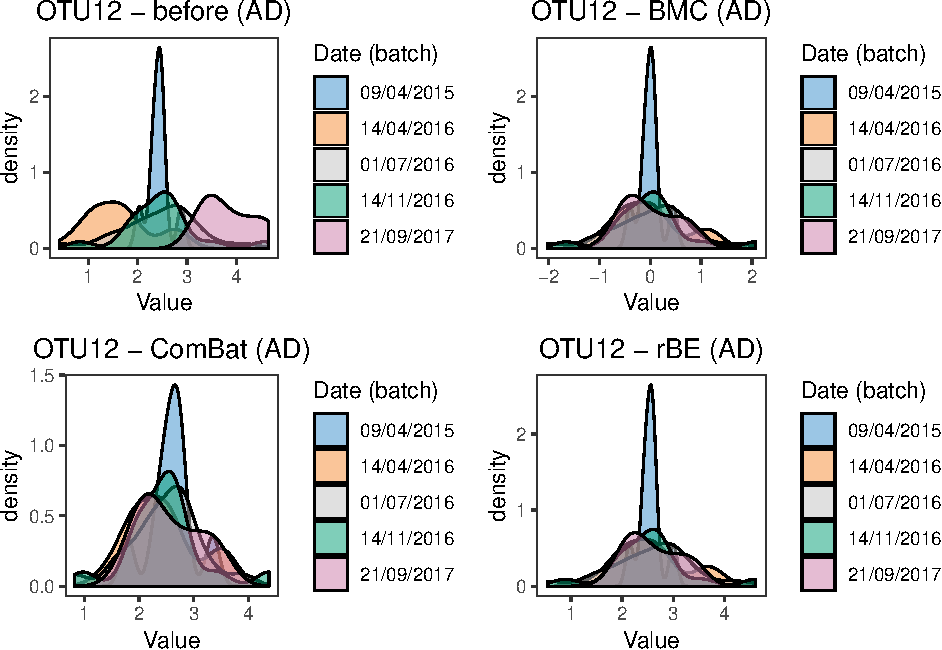
\includegraphics{vignette_files/figure-latex/unnamed-chunk-47-1.pdf}

\begin{Shaded}
\begin{Highlighting}[]
\KeywordTok{grid.arrange}\NormalTok{(plot.sponge.before, plot.sponge.percentile, plot.sponge.svd,}\DataTypeTok{ncol=}\DecValTok{2}\NormalTok{)}
\end{Highlighting}
\end{Shaded}

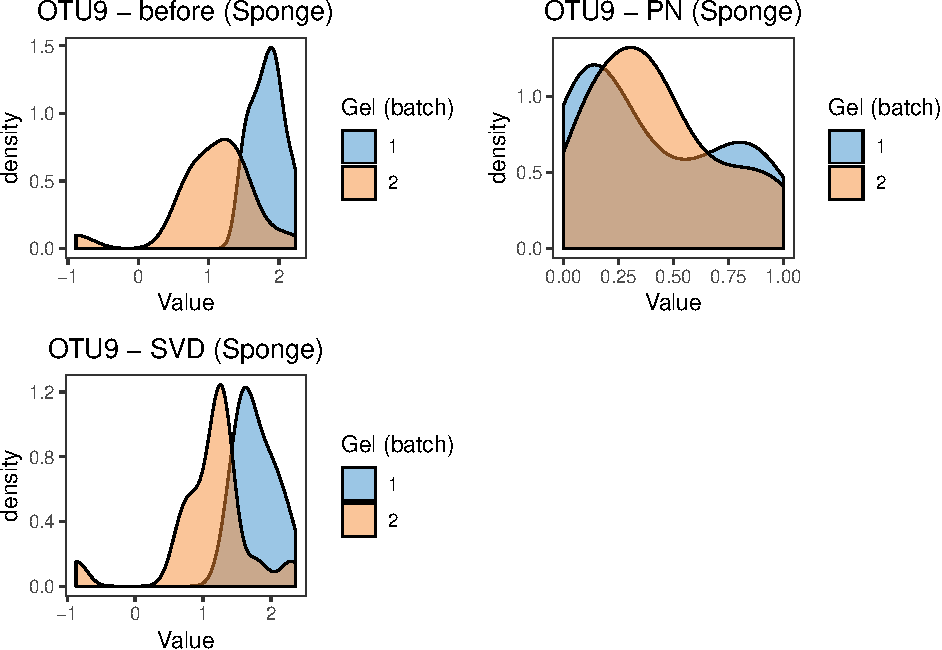
\includegraphics{vignette_files/figure-latex/unnamed-chunk-47-2.pdf}

\begin{Shaded}
\begin{Highlighting}[]
\NormalTok{######### p-values}
\NormalTok{linearm.sponge.before =}\StringTok{ }\KeywordTok{lm}\NormalTok{(sponge.tss.clr[,}\DecValTok{9}\NormalTok{]}\OperatorTok{~}\StringTok{ }\NormalTok{sponge.trt }\OperatorTok{+}\StringTok{ }\NormalTok{sponge.batch)}
\KeywordTok{summary}\NormalTok{(linearm.sponge.before)}
\end{Highlighting}
\end{Shaded}

\begin{verbatim}
## 
## Call:
## lm(formula = sponge.tss.clr[, 9] ~ sponge.trt + sponge.batch)
## 
## Residuals:
##      Min       1Q   Median       3Q      Max 
## -1.87967 -0.24705  0.04588  0.24492  1.00757 
## 
## Coefficients:
##               Estimate Std. Error t value Pr(>|t|)    
## (Intercept)     1.7849     0.1497  11.922 1.06e-12 ***
## sponge.trtE     0.1065     0.1729   0.616    0.543    
## sponge.batch2  -0.7910     0.1729  -4.575 8.24e-05 ***
## ---
## Signif. codes:  0 '***' 0.001 '**' 0.01 '*' 0.05 '.' 0.1 ' ' 1
## 
## Residual standard error: 0.489 on 29 degrees of freedom
## Multiple R-squared:  0.4236, Adjusted R-squared:  0.3839 
## F-statistic: 10.66 on 2 and 29 DF,  p-value: 0.0003391
\end{verbatim}

\begin{Shaded}
\begin{Highlighting}[]
\NormalTok{linearm.sponge.bmc =}\StringTok{ }\KeywordTok{lm}\NormalTok{(sponge.bmc[,}\DecValTok{9}\NormalTok{]}\OperatorTok{~}\StringTok{ }\NormalTok{sponge.trt }\OperatorTok{+}\StringTok{ }\NormalTok{sponge.batch)}
\KeywordTok{summary}\NormalTok{(linearm.sponge.bmc)}
\end{Highlighting}
\end{Shaded}

\begin{verbatim}
## 
## Call:
## lm(formula = sponge.bmc[, 9] ~ sponge.trt + sponge.batch)
## 
## Residuals:
##      Min       1Q   Median       3Q      Max 
## -1.87967 -0.24705  0.04588  0.24492  1.00757 
## 
## Coefficients:
##                 Estimate Std. Error t value Pr(>|t|)
## (Intercept)   -5.323e-02  1.497e-01  -0.356    0.725
## sponge.trtE    1.065e-01  1.729e-01   0.616    0.543
## sponge.batch2  3.925e-17  1.729e-01   0.000    1.000
## 
## Residual standard error: 0.489 on 29 degrees of freedom
## Multiple R-squared:  0.01291,    Adjusted R-squared:  -0.05517 
## F-statistic: 0.1896 on 2 and 29 DF,  p-value: 0.8283
\end{verbatim}

\begin{Shaded}
\begin{Highlighting}[]
\NormalTok{linearm.sponge.combat =}\StringTok{ }\KeywordTok{lm}\NormalTok{(sponge.combat[,}\DecValTok{9}\NormalTok{]}\OperatorTok{~}\StringTok{ }\NormalTok{sponge.trt }\OperatorTok{+}\StringTok{ }\NormalTok{sponge.batch)}
\KeywordTok{summary}\NormalTok{(linearm.sponge.combat)}
\end{Highlighting}
\end{Shaded}

\begin{verbatim}
## 
## Call:
## lm(formula = sponge.combat[, 9] ~ sponge.trt + sponge.batch)
## 
## Residuals:
##      Min       1Q   Median       3Q      Max 
## -1.64583 -0.22414  0.05092  0.24065  0.88585 
## 
## Coefficients:
##               Estimate Std. Error t value Pr(>|t|)    
## (Intercept)    1.46291    0.13491  10.844 1.02e-11 ***
## sponge.trtE    0.09081    0.15578   0.583    0.564    
## sponge.batch2 -0.16201    0.15578  -1.040    0.307    
## ---
## Signif. codes:  0 '***' 0.001 '**' 0.01 '*' 0.05 '.' 0.1 ' ' 1
## 
## Residual standard error: 0.4406 on 29 degrees of freedom
## Multiple R-squared:  0.04672,    Adjusted R-squared:  -0.01902 
## F-statistic: 0.7107 on 2 and 29 DF,  p-value: 0.4996
\end{verbatim}

\begin{Shaded}
\begin{Highlighting}[]
\NormalTok{linearm.sponge.limma =}\StringTok{ }\KeywordTok{lm}\NormalTok{(sponge.limma[,}\DecValTok{9}\NormalTok{]}\OperatorTok{~}\StringTok{ }\NormalTok{sponge.trt }\OperatorTok{+}\StringTok{ }\NormalTok{sponge.batch)}
\KeywordTok{summary}\NormalTok{(linearm.sponge.limma)}
\end{Highlighting}
\end{Shaded}

\begin{verbatim}
## 
## Call:
## lm(formula = sponge.limma[, 9] ~ sponge.trt + sponge.batch)
## 
## Residuals:
##      Min       1Q   Median       3Q      Max 
## -1.87967 -0.24705  0.04588  0.24492  1.00757 
## 
## Coefficients:
##                Estimate Std. Error t value Pr(>|t|)    
## (Intercept)   1.389e+00  1.497e-01   9.280 3.49e-10 ***
## sponge.trtE   1.065e-01  1.729e-01   0.616    0.543    
## sponge.batch2 2.355e-16  1.729e-01   0.000    1.000    
## ---
## Signif. codes:  0 '***' 0.001 '**' 0.01 '*' 0.05 '.' 0.1 ' ' 1
## 
## Residual standard error: 0.489 on 29 degrees of freedom
## Multiple R-squared:  0.01291,    Adjusted R-squared:  -0.05517 
## F-statistic: 0.1896 on 2 and 29 DF,  p-value: 0.8283
\end{verbatim}

\begin{Shaded}
\begin{Highlighting}[]
\NormalTok{linearm.sponge.percentile =}\StringTok{ }\KeywordTok{lm}\NormalTok{(sponge.percentile[,}\DecValTok{9}\NormalTok{]}\OperatorTok{~}\StringTok{ }\NormalTok{sponge.trt }\OperatorTok{+}\StringTok{ }\NormalTok{sponge.batch)}
\KeywordTok{summary}\NormalTok{(linearm.sponge.percentile)}
\end{Highlighting}
\end{Shaded}

\begin{verbatim}
## 
## Call:
## lm(formula = sponge.percentile[, 9] ~ sponge.trt + sponge.batch)
## 
## Residuals:
##     Min      1Q  Median      3Q     Max 
## -0.4531 -0.2070 -0.0625  0.1797  0.6562 
## 
## Coefficients:
##               Estimate Std. Error t value Pr(>|t|)    
## (Intercept)    0.48438    0.09515   5.090 1.97e-05 ***
## sponge.trtE   -0.17187    0.10987  -1.564    0.129    
## sponge.batch2  0.03125    0.10987   0.284    0.778    
## ---
## Signif. codes:  0 '***' 0.001 '**' 0.01 '*' 0.05 '.' 0.1 ' ' 1
## 
## Residual standard error: 0.3108 on 29 degrees of freedom
## Multiple R-squared:  0.08018,    Adjusted R-squared:  0.01674 
## F-statistic: 1.264 on 2 and 29 DF,  p-value: 0.2976
\end{verbatim}

\begin{Shaded}
\begin{Highlighting}[]
\NormalTok{linearm.sponge.svd =}\StringTok{ }\KeywordTok{lm}\NormalTok{(sponge.svd[,}\DecValTok{9}\NormalTok{]}\OperatorTok{~}\StringTok{ }\NormalTok{sponge.trt }\OperatorTok{+}\StringTok{ }\NormalTok{sponge.batch)}
\KeywordTok{summary}\NormalTok{(linearm.sponge.svd)}
\end{Highlighting}
\end{Shaded}

\begin{verbatim}
## 
## Call:
## lm(formula = sponge.svd[, 9] ~ sponge.trt + sponge.batch)
## 
## Residuals:
##      Min       1Q   Median       3Q      Max 
## -1.82982 -0.27539  0.05228  0.28204  1.05932 
## 
## Coefficients:
##               Estimate Std. Error t value Pr(>|t|)    
## (Intercept)     1.6433     0.1526  10.766 1.21e-11 ***
## sponge.trtE     0.2817     0.1763   1.598  0.12085    
## sponge.batch2  -0.6831     0.1763  -3.875  0.00056 ***
## ---
## Signif. codes:  0 '***' 0.001 '**' 0.01 '*' 0.05 '.' 0.1 ' ' 1
## 
## Residual standard error: 0.4985 on 29 degrees of freedom
## Multiple R-squared:  0.3773, Adjusted R-squared:  0.3344 
## F-statistic: 8.787 on 2 and 29 DF,  p-value: 0.001039
\end{verbatim}

\begin{Shaded}
\begin{Highlighting}[]
\NormalTok{##################}
\CommentTok{# ad data}

\CommentTok{# boxplot}
\NormalTok{ad.before.df =}\StringTok{ }\KeywordTok{data.frame}\NormalTok{(}\DataTypeTok{value =}\NormalTok{ ad.tss.clr[,}\DecValTok{1}\NormalTok{], }\DataTypeTok{batch =}\NormalTok{ ad.batch)}

\NormalTok{ad.before.boxplot <-}\StringTok{ }\KeywordTok{box_plot_fun}\NormalTok{(}\DataTypeTok{data =}\NormalTok{ ad.before.df,}\DataTypeTok{x=}\NormalTok{ad.before.df}\OperatorTok{$}\NormalTok{batch,}
             \DataTypeTok{y=}\NormalTok{ad.before.df}\OperatorTok{$}\NormalTok{value,}\DataTypeTok{title =} \StringTok{'OTU12 - before (AD)'}\NormalTok{,}
             \DataTypeTok{batch.legend.title =} \StringTok{'Date (batch)'}\NormalTok{,}
             \DataTypeTok{x.angle =} \DecValTok{45}\NormalTok{, }\DataTypeTok{x.hjust =} \DecValTok{1}\NormalTok{)}


\NormalTok{ad.bmc.df =}\StringTok{ }\KeywordTok{data.frame}\NormalTok{(}\DataTypeTok{value =}\NormalTok{ ad.bmc[,}\DecValTok{1}\NormalTok{], }\DataTypeTok{batch =}\NormalTok{ ad.batch)}

\NormalTok{ad.bmc.boxplot <-}\StringTok{ }\KeywordTok{box_plot_fun}\NormalTok{(}\DataTypeTok{data =}\NormalTok{ ad.bmc.df,}\DataTypeTok{x=}\NormalTok{ad.bmc.df}\OperatorTok{$}\NormalTok{batch,}
             \DataTypeTok{y=}\NormalTok{ad.bmc.df}\OperatorTok{$}\NormalTok{value,}\DataTypeTok{title =} \StringTok{'OTU12 - BMC (AD)'}\NormalTok{,}
             \DataTypeTok{batch.legend.title =} \StringTok{'Date (batch)'}\NormalTok{,}
             \DataTypeTok{x.angle =} \DecValTok{45}\NormalTok{, }\DataTypeTok{x.hjust =} \DecValTok{1}\NormalTok{)}


\NormalTok{ad.combat.df =}\StringTok{ }\KeywordTok{data.frame}\NormalTok{(}\DataTypeTok{value =}\NormalTok{ ad.combat[,}\DecValTok{1}\NormalTok{], }\DataTypeTok{batch =}\NormalTok{ ad.batch)}

\NormalTok{ad.combat.boxplot <-}\StringTok{ }\KeywordTok{box_plot_fun}\NormalTok{(}\DataTypeTok{data =}\NormalTok{ ad.combat.df,}\DataTypeTok{x=}\NormalTok{ad.combat.df}\OperatorTok{$}\NormalTok{batch,}
             \DataTypeTok{y=}\NormalTok{ad.combat.df}\OperatorTok{$}\NormalTok{value,}\DataTypeTok{title =} \StringTok{'OTU12 - ComBat (AD)'}\NormalTok{,}
             \DataTypeTok{batch.legend.title =} \StringTok{'Date (batch)'}\NormalTok{,}
             \DataTypeTok{x.angle =} \DecValTok{45}\NormalTok{, }\DataTypeTok{x.hjust =} \DecValTok{1}\NormalTok{)}

\NormalTok{ad.limma.df =}\StringTok{ }\KeywordTok{data.frame}\NormalTok{(}\DataTypeTok{value =}\NormalTok{ ad.limma[,}\DecValTok{1}\NormalTok{], }\DataTypeTok{batch =}\NormalTok{ ad.batch)}

\NormalTok{ad.limma.boxplot <-}\StringTok{ }\KeywordTok{box_plot_fun}\NormalTok{(}\DataTypeTok{data =}\NormalTok{ ad.limma.df,}\DataTypeTok{x=}\NormalTok{ad.limma.df}\OperatorTok{$}\NormalTok{batch,}
             \DataTypeTok{y=}\NormalTok{ad.limma.df}\OperatorTok{$}\NormalTok{value,}\DataTypeTok{title =} \StringTok{'OTU12 - rBE (AD)'}\NormalTok{,}
             \DataTypeTok{batch.legend.title =} \StringTok{'Date (batch)'}\NormalTok{,}
             \DataTypeTok{x.angle =} \DecValTok{45}\NormalTok{, }\DataTypeTok{x.hjust =} \DecValTok{1}\NormalTok{)}


\NormalTok{ad.percentile.df =}\StringTok{ }\KeywordTok{data.frame}\NormalTok{(}\DataTypeTok{value =}\NormalTok{ ad.percentile[,}\DecValTok{1}\NormalTok{], }\DataTypeTok{batch =}\NormalTok{ ad.batch)}

\NormalTok{ad.percentile.boxplot <-}\StringTok{ }\KeywordTok{box_plot_fun}\NormalTok{(}\DataTypeTok{data =}\NormalTok{ ad.percentile.df,}\DataTypeTok{x=}\NormalTok{ad.percentile.df}\OperatorTok{$}\NormalTok{batch,}
             \DataTypeTok{y=}\NormalTok{ad.percentile.df}\OperatorTok{$}\NormalTok{value,}\DataTypeTok{title =} \StringTok{'OTU12 - PN (AD)'}\NormalTok{,}
             \DataTypeTok{batch.legend.title =} \StringTok{'Date (batch)'}\NormalTok{,}
             \DataTypeTok{x.angle =} \DecValTok{45}\NormalTok{, }\DataTypeTok{x.hjust =} \DecValTok{1}\NormalTok{)}

\NormalTok{ad.svd.df =}\StringTok{ }\KeywordTok{data.frame}\NormalTok{(}\DataTypeTok{value =}\NormalTok{ ad.svd[,}\DecValTok{1}\NormalTok{], }\DataTypeTok{batch =}\NormalTok{ ad.batch)}

\NormalTok{ad.svd.boxplot <-}\StringTok{ }\KeywordTok{box_plot_fun}\NormalTok{(}\DataTypeTok{data =}\NormalTok{ ad.svd.df,}\DataTypeTok{x=}\NormalTok{ad.svd.df}\OperatorTok{$}\NormalTok{batch,}
             \DataTypeTok{y=}\NormalTok{ad.svd.df}\OperatorTok{$}\NormalTok{value,}\DataTypeTok{title =} \StringTok{'OTU12 - SVD (AD)'}\NormalTok{,}
             \DataTypeTok{batch.legend.title =} \StringTok{'Date (batch)'}\NormalTok{,}
             \DataTypeTok{x.angle =} \DecValTok{45}\NormalTok{, }\DataTypeTok{x.hjust =} \DecValTok{1}\NormalTok{)}

\NormalTok{ad.ruv.df =}\StringTok{ }\KeywordTok{data.frame}\NormalTok{(}\DataTypeTok{value =}\NormalTok{ ad.ruv[,}\DecValTok{1}\NormalTok{], }\DataTypeTok{batch =}\NormalTok{ ad.batch)}

\NormalTok{ad.ruv.boxplot <-}\StringTok{ }\KeywordTok{box_plot_fun}\NormalTok{(}\DataTypeTok{data =}\NormalTok{ ad.ruv.df,}\DataTypeTok{x=}\NormalTok{ad.ruv.df}\OperatorTok{$}\NormalTok{batch,}
             \DataTypeTok{y=}\NormalTok{ad.ruv.df}\OperatorTok{$}\NormalTok{value,}\DataTypeTok{title =} \StringTok{'OTU12 - RUVIII (AD)'}\NormalTok{,}
             \DataTypeTok{batch.legend.title =} \StringTok{'Date (batch)'}\NormalTok{,}
             \DataTypeTok{x.angle =} \DecValTok{45}\NormalTok{, }\DataTypeTok{x.hjust =} \DecValTok{1}\NormalTok{)}
\end{Highlighting}
\end{Shaded}

\begin{Shaded}
\begin{Highlighting}[]
\KeywordTok{grid.arrange}\NormalTok{(ad.before.boxplot, ad.bmc.boxplot, ad.combat.boxplot, ad.limma.boxplot,}\DataTypeTok{ncol=}\DecValTok{2}\NormalTok{)}
\end{Highlighting}
\end{Shaded}

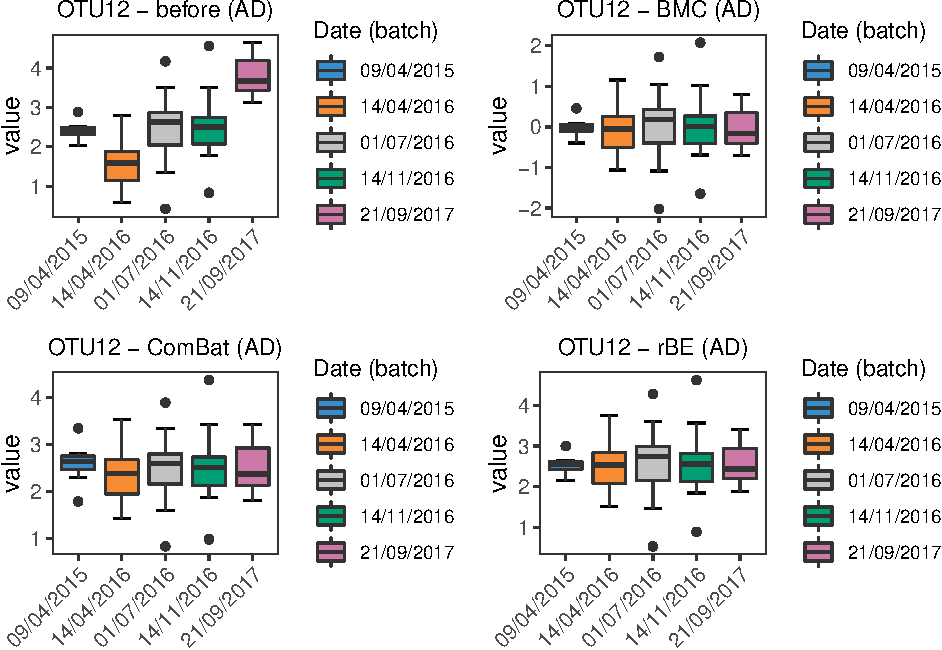
\includegraphics{vignette_files/figure-latex/unnamed-chunk-49-1.pdf}

\begin{Shaded}
\begin{Highlighting}[]
\KeywordTok{grid.arrange}\NormalTok{(ad.before.boxplot, ad.percentile.boxplot,ad.svd.boxplot,ad.ruv.boxplot,}\DataTypeTok{ncol=}\DecValTok{2}\NormalTok{)}
\end{Highlighting}
\end{Shaded}

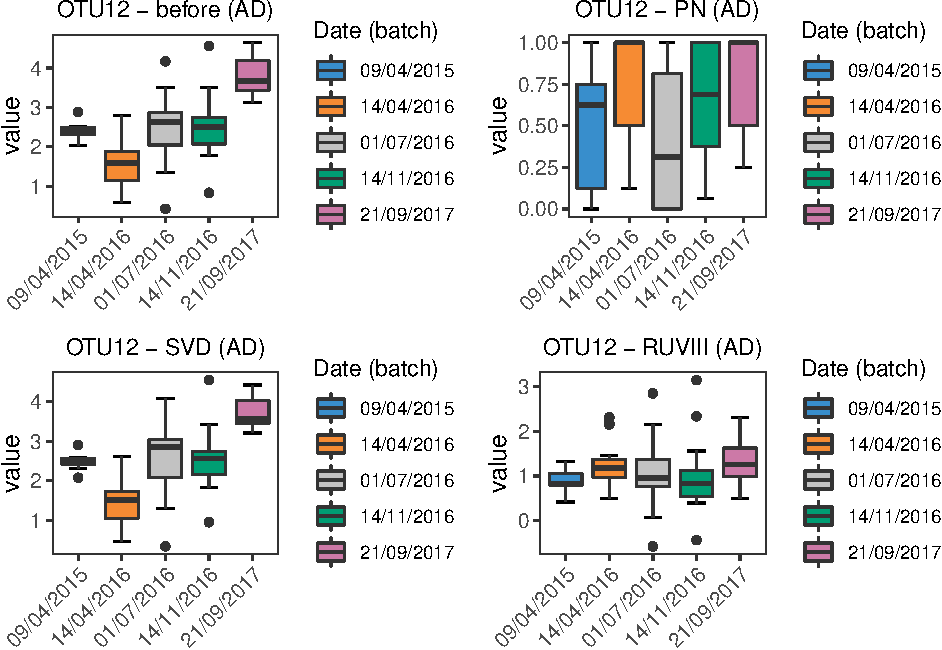
\includegraphics{vignette_files/figure-latex/unnamed-chunk-49-2.pdf}

\begin{Shaded}
\begin{Highlighting}[]
\CommentTok{# density plot}
\CommentTok{# before}
\NormalTok{plot.ad.before =}\StringTok{ }\KeywordTok{ggplot}\NormalTok{(ad.before.df, }\KeywordTok{aes}\NormalTok{(}\DataTypeTok{x =}\NormalTok{ value, }\DataTypeTok{fill =}\NormalTok{ batch)) }\OperatorTok{+}\StringTok{ }\KeywordTok{geom_density}\NormalTok{(}\DataTypeTok{alpha =} \FloatTok{0.5}\NormalTok{) }\OperatorTok{+}\StringTok{ }\KeywordTok{scale_fill_manual}\NormalTok{(}\DataTypeTok{values=}\KeywordTok{color.mixo}\NormalTok{(}\DecValTok{1}\OperatorTok{:}\DecValTok{10}\NormalTok{)) }\OperatorTok{+}\StringTok{ }\KeywordTok{labs}\NormalTok{(}\DataTypeTok{title =} \StringTok{'OTU12 - before (AD)'}\NormalTok{,}\DataTypeTok{x =} \StringTok{'Value'}\NormalTok{,}\DataTypeTok{fill =} \StringTok{'Date (batch)'}\NormalTok{) }\OperatorTok{+}\StringTok{ }\KeywordTok{theme_bw}\NormalTok{() }\OperatorTok{+}\StringTok{ }\KeywordTok{theme}\NormalTok{(}\DataTypeTok{plot.title =} \KeywordTok{element_text}\NormalTok{(}\DataTypeTok{hjust=}\FloatTok{0.5}\NormalTok{), }\DataTypeTok{panel.grid =} \KeywordTok{element_blank}\NormalTok{())}

\CommentTok{# BMC}
\NormalTok{plot.ad.bmc =}\StringTok{ }\KeywordTok{ggplot}\NormalTok{(ad.bmc.df, }\KeywordTok{aes}\NormalTok{(}\DataTypeTok{x =}\NormalTok{ value, }\DataTypeTok{fill =}\NormalTok{ batch)) }\OperatorTok{+}\StringTok{ }\KeywordTok{geom_density}\NormalTok{(}\DataTypeTok{alpha =} \FloatTok{0.5}\NormalTok{) }\OperatorTok{+}\StringTok{ }\KeywordTok{scale_fill_manual}\NormalTok{(}\DataTypeTok{values=}\KeywordTok{color.mixo}\NormalTok{(}\DecValTok{1}\OperatorTok{:}\DecValTok{10}\NormalTok{)) }\OperatorTok{+}\StringTok{ }\KeywordTok{labs}\NormalTok{(}\DataTypeTok{title =} \StringTok{'OTU12 - BMC (AD)'}\NormalTok{,}\DataTypeTok{x =} \StringTok{'Value'}\NormalTok{,}\DataTypeTok{fill =} \StringTok{'Date (batch)'}\NormalTok{) }\OperatorTok{+}\StringTok{ }\KeywordTok{theme_bw}\NormalTok{() }\OperatorTok{+}\StringTok{ }\KeywordTok{theme}\NormalTok{(}\DataTypeTok{plot.title =} \KeywordTok{element_text}\NormalTok{(}\DataTypeTok{hjust=}\FloatTok{0.5}\NormalTok{), }\DataTypeTok{panel.grid =} \KeywordTok{element_blank}\NormalTok{())}


\CommentTok{# ComBat}
\NormalTok{plot.ad.combat =}\StringTok{ }\KeywordTok{ggplot}\NormalTok{(ad.combat.df, }\KeywordTok{aes}\NormalTok{(}\DataTypeTok{x =}\NormalTok{ value, }\DataTypeTok{fill =}\NormalTok{ batch)) }\OperatorTok{+}\StringTok{ }\KeywordTok{geom_density}\NormalTok{(}\DataTypeTok{alpha =} \FloatTok{0.5}\NormalTok{) }\OperatorTok{+}\StringTok{ }\KeywordTok{scale_fill_manual}\NormalTok{(}\DataTypeTok{values=}\KeywordTok{color.mixo}\NormalTok{(}\DecValTok{1}\OperatorTok{:}\DecValTok{10}\NormalTok{)) }\OperatorTok{+}\StringTok{ }\KeywordTok{labs}\NormalTok{(}\DataTypeTok{title =} \StringTok{'OTU12 - ComBat (AD)'}\NormalTok{,}\DataTypeTok{x =} \StringTok{'Value'}\NormalTok{,}\DataTypeTok{fill =} \StringTok{'Date (batch)'}\NormalTok{) }\OperatorTok{+}\StringTok{ }\KeywordTok{theme_bw}\NormalTok{() }\OperatorTok{+}\StringTok{ }\KeywordTok{theme}\NormalTok{(}\DataTypeTok{plot.title =} \KeywordTok{element_text}\NormalTok{(}\DataTypeTok{hjust=}\FloatTok{0.5}\NormalTok{), }\DataTypeTok{panel.grid =} \KeywordTok{element_blank}\NormalTok{())}


\CommentTok{# removeBatchEffect}
\NormalTok{plot.ad.limma =}\StringTok{ }\KeywordTok{ggplot}\NormalTok{(ad.limma.df, }\KeywordTok{aes}\NormalTok{(}\DataTypeTok{x =}\NormalTok{ value, }\DataTypeTok{fill =}\NormalTok{ batch)) }\OperatorTok{+}\StringTok{ }\KeywordTok{geom_density}\NormalTok{(}\DataTypeTok{alpha =} \FloatTok{0.5}\NormalTok{) }\OperatorTok{+}\StringTok{ }\KeywordTok{scale_fill_manual}\NormalTok{(}\DataTypeTok{values=}\KeywordTok{color.mixo}\NormalTok{(}\DecValTok{1}\OperatorTok{:}\DecValTok{10}\NormalTok{)) }\OperatorTok{+}\StringTok{ }\KeywordTok{labs}\NormalTok{(}\DataTypeTok{title =} \StringTok{'OTU12 - rBE (AD)'}\NormalTok{,}\DataTypeTok{x =} \StringTok{'Value'}\NormalTok{,}\DataTypeTok{fill =} \StringTok{'Date (batch)'}\NormalTok{) }\OperatorTok{+}\StringTok{ }\KeywordTok{theme_bw}\NormalTok{() }\OperatorTok{+}\StringTok{ }\KeywordTok{theme}\NormalTok{(}\DataTypeTok{plot.title =} \KeywordTok{element_text}\NormalTok{(}\DataTypeTok{hjust=}\FloatTok{0.5}\NormalTok{), }\DataTypeTok{panel.grid =} \KeywordTok{element_blank}\NormalTok{())}


\CommentTok{# percentile norm}
\NormalTok{plot.ad.percentile =}\StringTok{ }\KeywordTok{ggplot}\NormalTok{(ad.percentile.df, }\KeywordTok{aes}\NormalTok{(}\DataTypeTok{x =}\NormalTok{ value, }\DataTypeTok{fill =}\NormalTok{ batch)) }\OperatorTok{+}\StringTok{ }\KeywordTok{geom_density}\NormalTok{(}\DataTypeTok{alpha =} \FloatTok{0.5}\NormalTok{) }\OperatorTok{+}\StringTok{ }\KeywordTok{scale_fill_manual}\NormalTok{(}\DataTypeTok{values=}\KeywordTok{color.mixo}\NormalTok{(}\DecValTok{1}\OperatorTok{:}\DecValTok{10}\NormalTok{)) }\OperatorTok{+}\StringTok{ }\KeywordTok{labs}\NormalTok{(}\DataTypeTok{title =} \StringTok{'OTU12 - PN (AD)'}\NormalTok{,}\DataTypeTok{x =} \StringTok{'Value'}\NormalTok{,}\DataTypeTok{fill =} \StringTok{'Date (batch)'}\NormalTok{) }\OperatorTok{+}\StringTok{ }\KeywordTok{theme_bw}\NormalTok{() }\OperatorTok{+}\StringTok{ }\KeywordTok{theme}\NormalTok{(}\DataTypeTok{plot.title =} \KeywordTok{element_text}\NormalTok{(}\DataTypeTok{hjust=}\FloatTok{0.5}\NormalTok{), }\DataTypeTok{panel.grid =} \KeywordTok{element_blank}\NormalTok{())}


\CommentTok{# SVD}
\NormalTok{plot.ad.svd =}\StringTok{ }\KeywordTok{ggplot}\NormalTok{(ad.svd.df, }\KeywordTok{aes}\NormalTok{(}\DataTypeTok{x =}\NormalTok{ value, }\DataTypeTok{fill =}\NormalTok{ batch)) }\OperatorTok{+}\StringTok{ }\KeywordTok{geom_density}\NormalTok{(}\DataTypeTok{alpha =} \FloatTok{0.5}\NormalTok{) }\OperatorTok{+}\StringTok{ }\KeywordTok{scale_fill_manual}\NormalTok{(}\DataTypeTok{values=}\KeywordTok{color.mixo}\NormalTok{(}\DecValTok{1}\OperatorTok{:}\DecValTok{10}\NormalTok{)) }\OperatorTok{+}\StringTok{ }\KeywordTok{labs}\NormalTok{(}\DataTypeTok{title =} \StringTok{'OTU12 - SVD (AD)'}\NormalTok{,}\DataTypeTok{x =} \StringTok{'Value'}\NormalTok{,}\DataTypeTok{fill =} \StringTok{'Date (batch)'}\NormalTok{) }\OperatorTok{+}\StringTok{ }\KeywordTok{theme_bw}\NormalTok{() }\OperatorTok{+}\StringTok{ }\KeywordTok{theme}\NormalTok{(}\DataTypeTok{plot.title =} \KeywordTok{element_text}\NormalTok{(}\DataTypeTok{hjust=}\FloatTok{0.5}\NormalTok{), }\DataTypeTok{panel.grid =} \KeywordTok{element_blank}\NormalTok{())}


\CommentTok{# RUVIII}
\NormalTok{plot.ad.ruv =}\StringTok{ }\KeywordTok{ggplot}\NormalTok{(ad.ruv.df, }\KeywordTok{aes}\NormalTok{(}\DataTypeTok{x =}\NormalTok{ value, }\DataTypeTok{fill =}\NormalTok{ batch)) }\OperatorTok{+}\StringTok{ }\KeywordTok{geom_density}\NormalTok{(}\DataTypeTok{alpha =} \FloatTok{0.5}\NormalTok{) }\OperatorTok{+}\StringTok{ }\KeywordTok{scale_fill_manual}\NormalTok{(}\DataTypeTok{values=}\KeywordTok{color.mixo}\NormalTok{(}\DecValTok{1}\OperatorTok{:}\DecValTok{10}\NormalTok{)) }\OperatorTok{+}\StringTok{ }\KeywordTok{labs}\NormalTok{(}\DataTypeTok{title =} \StringTok{'OTU12 - RUVIII (AD)'}\NormalTok{,}\DataTypeTok{x =} \StringTok{'Value'}\NormalTok{,}\DataTypeTok{fill =} \StringTok{'Date (batch)'}\NormalTok{) }\OperatorTok{+}\StringTok{ }\KeywordTok{theme_bw}\NormalTok{() }\OperatorTok{+}\StringTok{ }\KeywordTok{theme}\NormalTok{(}\DataTypeTok{plot.title =} \KeywordTok{element_text}\NormalTok{(}\DataTypeTok{hjust=}\FloatTok{0.5}\NormalTok{), }\DataTypeTok{panel.grid =} \KeywordTok{element_blank}\NormalTok{())}
\end{Highlighting}
\end{Shaded}

\begin{Shaded}
\begin{Highlighting}[]
\KeywordTok{grid.arrange}\NormalTok{(plot.ad.before, plot.ad.bmc, plot.ad.combat,plot.ad.limma,}\DataTypeTok{ncol=}\DecValTok{2}\NormalTok{)}
\end{Highlighting}
\end{Shaded}

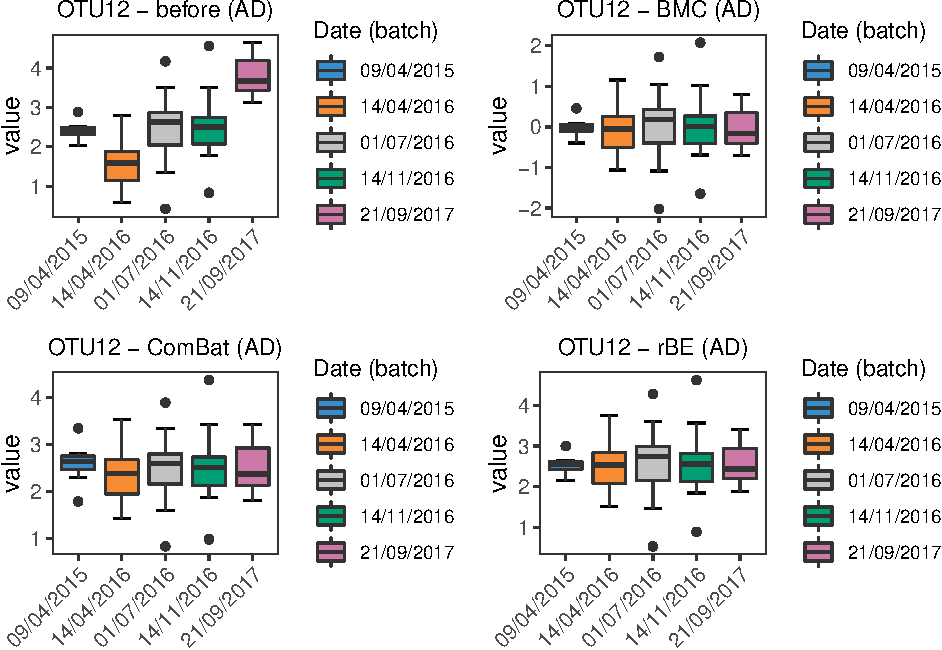
\includegraphics{vignette_files/figure-latex/unnamed-chunk-51-1.pdf}

\begin{Shaded}
\begin{Highlighting}[]
\KeywordTok{grid.arrange}\NormalTok{(plot.ad.before, plot.ad.percentile, plot.ad.svd,plot.ad.ruv, }\DataTypeTok{ncol=}\DecValTok{2}\NormalTok{)}
\end{Highlighting}
\end{Shaded}

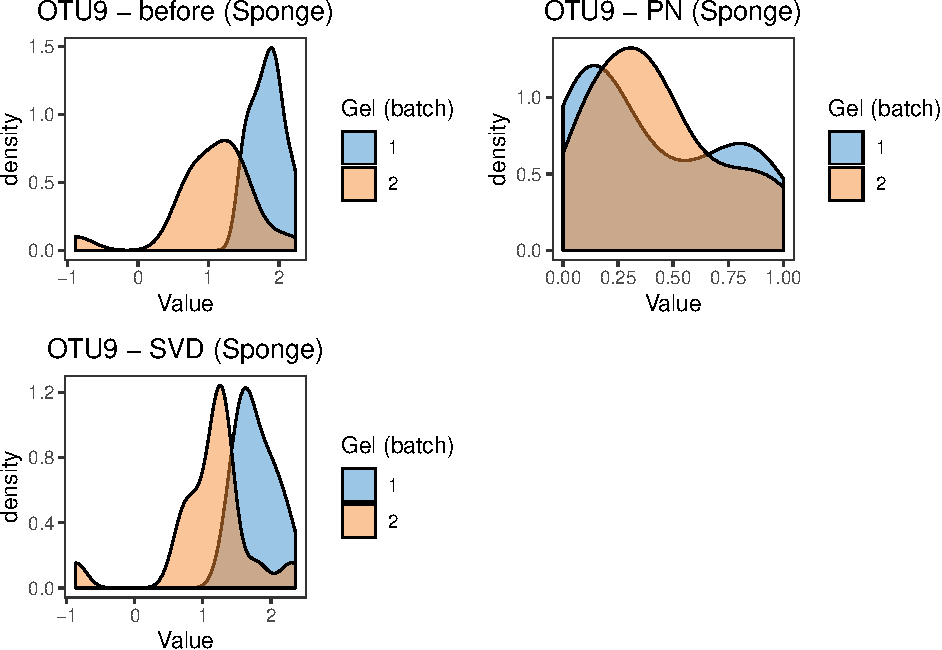
\includegraphics{vignette_files/figure-latex/unnamed-chunk-51-2.pdf}

\begin{Shaded}
\begin{Highlighting}[]
\CommentTok{#p-values}
\NormalTok{linearm.ad.before =}\StringTok{ }\KeywordTok{lm}\NormalTok{(ad.tss.clr[,}\DecValTok{1}\NormalTok{]}\OperatorTok{~}\StringTok{ }\NormalTok{ad.trt }\OperatorTok{+}\StringTok{ }\NormalTok{ad.batch)}
\KeywordTok{anova}\NormalTok{(linearm.ad.before)}
\end{Highlighting}
\end{Shaded}

\begin{verbatim}
## Analysis of Variance Table
## 
## Response: ad.tss.clr[, 1]
##           Df Sum Sq Mean Sq F value    Pr(>F)    
## ad.trt     1  1.460  1.4605  3.1001   0.08272 .  
## ad.batch   4 32.889  8.2222 17.4532 6.168e-10 ***
## Residuals 69 32.506  0.4711                      
## ---
## Signif. codes:  0 '***' 0.001 '**' 0.01 '*' 0.05 '.' 0.1 ' ' 1
\end{verbatim}

\begin{Shaded}
\begin{Highlighting}[]
\KeywordTok{summary}\NormalTok{(linearm.ad.before)}
\end{Highlighting}
\end{Shaded}

\begin{verbatim}
## 
## Call:
## lm(formula = ad.tss.clr[, 1] ~ ad.trt + ad.batch)
## 
## Residuals:
##      Min       1Q   Median       3Q      Max 
## -2.09885 -0.39613 -0.00381  0.36645  1.98185 
## 
## Coefficients:
##                     Estimate Std. Error t value Pr(>|t|)    
## (Intercept)         2.311213   0.247768   9.328 7.57e-14 ***
## ad.trt1-2           0.203619   0.171183   1.189  0.23833    
## ad.batch14/04/2016 -0.828100   0.287918  -2.876  0.00535 ** 
## ad.batch01/07/2016  0.007239   0.273672   0.026  0.97897    
## ad.batch14/11/2016  0.062689   0.282978   0.222  0.82533    
## ad.batch21/09/2017  1.361132   0.306373   4.443 3.30e-05 ***
## ---
## Signif. codes:  0 '***' 0.001 '**' 0.01 '*' 0.05 '.' 0.1 ' ' 1
## 
## Residual standard error: 0.6864 on 69 degrees of freedom
## Multiple R-squared:  0.5138, Adjusted R-squared:  0.4786 
## F-statistic: 14.58 on 5 and 69 DF,  p-value: 9.665e-10
\end{verbatim}

\begin{Shaded}
\begin{Highlighting}[]
\NormalTok{linearm.ad.bmc =}\StringTok{ }\KeywordTok{lm}\NormalTok{(ad.bmc[,}\DecValTok{1}\NormalTok{]}\OperatorTok{~}\StringTok{ }\NormalTok{ad.trt }\OperatorTok{+}\StringTok{ }\NormalTok{ad.batch)}
\KeywordTok{anova}\NormalTok{(linearm.ad.bmc)}
\end{Highlighting}
\end{Shaded}

\begin{verbatim}
## Analysis of Variance Table
## 
## Response: ad.bmc[, 1]
##           Df Sum Sq Mean Sq F value Pr(>F)
## ad.trt     1  0.631 0.63084  1.3391 0.2512
## ad.batch   4  0.036 0.00893  0.0190 0.9993
## Residuals 69 32.506 0.47110
\end{verbatim}

\begin{Shaded}
\begin{Highlighting}[]
\KeywordTok{summary}\NormalTok{(linearm.ad.bmc)}
\end{Highlighting}
\end{Shaded}

\begin{verbatim}
## 
## Call:
## lm(formula = ad.bmc[, 1] ~ ad.trt + ad.batch)
## 
## Residuals:
##      Min       1Q   Median       3Q      Max 
## -2.09885 -0.39613 -0.00381  0.36645  1.98185 
## 
## Coefficients:
##                     Estimate Std. Error t value Pr(>|t|)
## (Intercept)        -0.113122   0.247768  -0.457    0.649
## ad.trt1-2           0.203619   0.171183   1.189    0.238
## ad.batch14/04/2016 -0.039593   0.287918  -0.138    0.891
## ad.batch01/07/2016 -0.012928   0.273672  -0.047    0.962
## ad.batch14/11/2016  0.005323   0.282978   0.019    0.985
## ad.batch21/09/2017 -0.056561   0.306373  -0.185    0.854
## 
## Residual standard error: 0.6864 on 69 degrees of freedom
## Multiple R-squared:  0.02009,    Adjusted R-squared:  -0.05091 
## F-statistic: 0.283 on 5 and 69 DF,  p-value: 0.9209
\end{verbatim}

\begin{Shaded}
\begin{Highlighting}[]
\NormalTok{linearm.ad.combat =}\StringTok{ }\KeywordTok{lm}\NormalTok{(ad.combat[,}\DecValTok{1}\NormalTok{]}\OperatorTok{~}\StringTok{ }\NormalTok{ad.trt }\OperatorTok{+}\StringTok{ }\NormalTok{ad.batch)}
\KeywordTok{anova}\NormalTok{(linearm.ad.combat)}
\end{Highlighting}
\end{Shaded}

\begin{verbatim}
## Analysis of Variance Table
## 
## Response: ad.combat[, 1]
##           Df  Sum Sq Mean Sq F value Pr(>F)
## ad.trt     1  0.6695 0.66954  1.6980 0.1969
## ad.batch   4  0.2373 0.05932  0.1504 0.9622
## Residuals 69 27.2080 0.39432
\end{verbatim}

\begin{Shaded}
\begin{Highlighting}[]
\KeywordTok{summary}\NormalTok{(linearm.ad.combat)}
\end{Highlighting}
\end{Shaded}

\begin{verbatim}
## 
## Call:
## lm(formula = ad.combat[, 1] ~ ad.trt + ad.batch)
## 
## Residuals:
##      Min       1Q   Median       3Q      Max 
## -1.72209 -0.38700 -0.00346  0.34754  1.79333 
## 
## Coefficients:
##                    Estimate Std. Error t value Pr(>|t|)    
## (Intercept)         2.46834    0.22668  10.889   <2e-16 ***
## ad.trt1-2           0.20995    0.15661   1.341    0.184    
## ad.batch14/04/2016 -0.19520    0.26341  -0.741    0.461    
## ad.batch01/07/2016 -0.12986    0.25038  -0.519    0.606    
## ad.batch14/11/2016 -0.09816    0.25889  -0.379    0.706    
## ad.batch21/09/2017 -0.08901    0.28030  -0.318    0.752    
## ---
## Signif. codes:  0 '***' 0.001 '**' 0.01 '*' 0.05 '.' 0.1 ' ' 1
## 
## Residual standard error: 0.6279 on 69 degrees of freedom
## Multiple R-squared:  0.03225,    Adjusted R-squared:  -0.03787 
## F-statistic: 0.4599 on 5 and 69 DF,  p-value: 0.8047
\end{verbatim}

\begin{Shaded}
\begin{Highlighting}[]
\NormalTok{linearm.ad.limma =}\StringTok{ }\KeywordTok{lm}\NormalTok{(ad.limma[,}\DecValTok{1}\NormalTok{]}\OperatorTok{~}\StringTok{ }\NormalTok{ad.trt }\OperatorTok{+}\StringTok{ }\NormalTok{ad.batch)}
\KeywordTok{anova}\NormalTok{(linearm.ad.limma)}
\end{Highlighting}
\end{Shaded}

\begin{verbatim}
## Analysis of Variance Table
## 
## Response: ad.limma[, 1]
##           Df Sum Sq Mean Sq F value Pr(>F)
## ad.trt     1  0.704 0.70428   1.495 0.2256
## ad.batch   4  0.000 0.00000   0.000 1.0000
## Residuals 69 32.506 0.47110
\end{verbatim}

\begin{Shaded}
\begin{Highlighting}[]
\KeywordTok{summary}\NormalTok{(linearm.ad.limma)}
\end{Highlighting}
\end{Shaded}

\begin{verbatim}
## 
## Call:
## lm(formula = ad.limma[, 1] ~ ad.trt + ad.batch)
## 
## Residuals:
##      Min       1Q   Median       3Q      Max 
## -2.09885 -0.39613 -0.00381  0.36645  1.98185 
## 
## Coefficients:
##                     Estimate Std. Error t value Pr(>|t|)    
## (Intercept)        2.432e+00  2.478e-01   9.815    1e-14 ***
## ad.trt1-2          2.036e-01  1.712e-01   1.189    0.238    
## ad.batch14/04/2016 2.561e-15  2.879e-01   0.000    1.000    
## ad.batch01/07/2016 1.175e-15  2.737e-01   0.000    1.000    
## ad.batch14/11/2016 1.116e-15  2.830e-01   0.000    1.000    
## ad.batch21/09/2017 2.973e-16  3.064e-01   0.000    1.000    
## ---
## Signif. codes:  0 '***' 0.001 '**' 0.01 '*' 0.05 '.' 0.1 ' ' 1
## 
## Residual standard error: 0.6864 on 69 degrees of freedom
## Multiple R-squared:  0.02121,    Adjusted R-squared:  -0.04972 
## F-statistic: 0.299 on 5 and 69 DF,  p-value: 0.9118
\end{verbatim}

\begin{Shaded}
\begin{Highlighting}[]
\NormalTok{linearm.ad.percentile =}\StringTok{ }\KeywordTok{lm}\NormalTok{(ad.percentile[,}\DecValTok{1}\NormalTok{]}\OperatorTok{~}\StringTok{ }\NormalTok{ad.trt }\OperatorTok{+}\StringTok{ }\NormalTok{ad.batch)}
\KeywordTok{anova}\NormalTok{(linearm.ad.percentile)}
\end{Highlighting}
\end{Shaded}

\begin{verbatim}
## Analysis of Variance Table
## 
## Response: ad.percentile[, 1]
##           Df Sum Sq Mean Sq F value  Pr(>F)  
## ad.trt     1 0.4670 0.46705  3.8934 0.05248 .
## ad.batch   4 1.7037 0.42592  3.5506 0.01081 *
## Residuals 69 8.2772 0.11996                  
## ---
## Signif. codes:  0 '***' 0.001 '**' 0.01 '*' 0.05 '.' 0.1 ' ' 1
\end{verbatim}

\begin{Shaded}
\begin{Highlighting}[]
\KeywordTok{summary}\NormalTok{(linearm.ad.percentile)}
\end{Highlighting}
\end{Shaded}

\begin{verbatim}
## 
## Call:
## lm(formula = ad.percentile[, 1] ~ ad.trt + ad.batch)
## 
## Residuals:
##     Min      1Q  Median      3Q     Max 
## -0.5560 -0.3126  0.1613  0.2029  0.6226 
## 
## Coefficients:
##                    Estimate Std. Error t value Pr(>|t|)    
## (Intercept)         0.43006    0.12503   3.440 0.000992 ***
## ad.trt1-2           0.12590    0.08638   1.457 0.149528    
## ad.batch14/04/2016  0.24115    0.14529   1.660 0.101497    
## ad.batch01/07/2016 -0.11514    0.13810  -0.834 0.407312    
## ad.batch14/11/2016  0.15770    0.14279   1.104 0.273254    
## ad.batch21/09/2017  0.25670    0.15460   1.660 0.101375    
## ---
## Signif. codes:  0 '***' 0.001 '**' 0.01 '*' 0.05 '.' 0.1 ' ' 1
## 
## Residual standard error: 0.3464 on 69 degrees of freedom
## Multiple R-squared:  0.2078, Adjusted R-squared:  0.1504 
## F-statistic: 3.619 on 5 and 69 DF,  p-value: 0.005766
\end{verbatim}

\begin{Shaded}
\begin{Highlighting}[]
\NormalTok{linearm.ad.svd =}\StringTok{ }\KeywordTok{lm}\NormalTok{(ad.svd[,}\DecValTok{1}\NormalTok{]}\OperatorTok{~}\StringTok{ }\NormalTok{ad.trt }\OperatorTok{+}\StringTok{ }\NormalTok{ad.batch)}
\KeywordTok{anova}\NormalTok{(linearm.ad.svd)}
\end{Highlighting}
\end{Shaded}

\begin{verbatim}
## Analysis of Variance Table
## 
## Response: ad.svd[, 1]
##           Df Sum Sq Mean Sq F value    Pr(>F)    
## ad.trt     1  0.222  0.2218  0.4841    0.4889    
## ad.batch   4 33.914  8.4784 18.5081 2.256e-10 ***
## Residuals 69 31.608  0.4581                      
## ---
## Signif. codes:  0 '***' 0.001 '**' 0.01 '*' 0.05 '.' 0.1 ' ' 1
\end{verbatim}

\begin{Shaded}
\begin{Highlighting}[]
\KeywordTok{summary}\NormalTok{(linearm.ad.svd)}
\end{Highlighting}
\end{Shaded}

\begin{verbatim}
## 
## Call:
## lm(formula = ad.svd[, 1] ~ ad.trt + ad.batch)
## 
## Residuals:
##      Min       1Q   Median       3Q      Max 
## -2.18899 -0.39114  0.00684  0.40400  1.98037 
## 
## Coefficients:
##                    Estimate Std. Error t value Pr(>|t|)    
## (Intercept)         2.45910    0.24432  10.065 3.57e-15 ***
## ad.trt1-2           0.05243    0.16880   0.311 0.757055    
## ad.batch14/04/2016 -0.97834    0.28391  -3.446 0.000973 ***
## ad.batch01/07/2016  0.02012    0.26987   0.075 0.940779    
## ad.batch14/11/2016  0.05321    0.27904   0.191 0.849320    
## ad.batch21/09/2017  1.24541    0.30211   4.122 0.000103 ***
## ---
## Signif. codes:  0 '***' 0.001 '**' 0.01 '*' 0.05 '.' 0.1 ' ' 1
## 
## Residual standard error: 0.6768 on 69 degrees of freedom
## Multiple R-squared:  0.5192, Adjusted R-squared:  0.4844 
## F-statistic:  14.9 on 5 and 69 DF,  p-value: 6.658e-10
\end{verbatim}

\begin{Shaded}
\begin{Highlighting}[]
\NormalTok{linearm.ad.ruv =}\StringTok{ }\KeywordTok{lm}\NormalTok{(ad.ruv[,}\DecValTok{1}\NormalTok{]}\OperatorTok{~}\StringTok{ }\NormalTok{ad.trt }\OperatorTok{+}\StringTok{ }\NormalTok{ad.batch)}
\KeywordTok{anova}\NormalTok{(linearm.ad.ruv)}
\end{Highlighting}
\end{Shaded}

\begin{verbatim}
## Analysis of Variance Table
## 
## Response: ad.ruv[, 1]
##           Df  Sum Sq Mean Sq F value  Pr(>F)  
## ad.trt     1  1.7759 1.77595  4.4258 0.03905 *
## ad.batch   4  1.3555 0.33888  0.8445 0.50179  
## Residuals 69 27.6877 0.40127                  
## ---
## Signif. codes:  0 '***' 0.001 '**' 0.01 '*' 0.05 '.' 0.1 ' ' 1
\end{verbatim}

\begin{Shaded}
\begin{Highlighting}[]
\KeywordTok{summary}\NormalTok{(linearm.ad.ruv)}
\end{Highlighting}
\end{Shaded}

\begin{verbatim}
## 
## Call:
## lm(formula = ad.ruv[, 1] ~ ad.trt + ad.batch)
## 
## Residuals:
##      Min       1Q   Median       3Q      Max 
## -1.69231 -0.31474 -0.06617  0.22934  2.04171 
## 
## Coefficients:
##                    Estimate Std. Error t value Pr(>|t|)   
## (Intercept)          0.7435     0.2287   3.251  0.00178 **
## ad.trt1-2            0.2599     0.1580   1.645  0.10455   
## ad.batch14/04/2016   0.3266     0.2657   1.229  0.22318   
## ad.batch01/07/2016   0.1115     0.2526   0.441  0.66027   
## ad.batch14/11/2016   0.1022     0.2612   0.391  0.69666   
## ad.batch21/09/2017   0.4022     0.2828   1.422  0.15942   
## ---
## Signif. codes:  0 '***' 0.001 '**' 0.01 '*' 0.05 '.' 0.1 ' ' 1
## 
## Residual standard error: 0.6335 on 69 degrees of freedom
## Multiple R-squared:  0.1016, Adjusted R-squared:  0.03651 
## F-statistic: 1.561 on 5 and 69 DF,  p-value: 0.1828
\end{verbatim}

\subsection{RLE plots}\label{rle-plots-1}

\begin{Shaded}
\begin{Highlighting}[]
\CommentTok{# sponge data}
\CommentTok{# before}

\NormalTok{###### BMC}
\NormalTok{sponge.bmc_c =}\StringTok{ }\NormalTok{sponge.bmc[sponge.trt }\OperatorTok{==}\StringTok{ 'C'}\NormalTok{,]}
\NormalTok{sponge.bmc_e =}\StringTok{ }\NormalTok{sponge.bmc[sponge.trt }\OperatorTok{==}\StringTok{ 'E'}\NormalTok{,] }

\NormalTok{###### ComBat}
\NormalTok{sponge.combat_c =}\StringTok{ }\NormalTok{sponge.combat[sponge.trt }\OperatorTok{==}\StringTok{ 'C'}\NormalTok{,]}
\NormalTok{sponge.combat_e =}\StringTok{ }\NormalTok{sponge.combat[sponge.trt }\OperatorTok{==}\StringTok{ 'E'}\NormalTok{,] }

\NormalTok{###### rBE}
\NormalTok{sponge.limma_c =}\StringTok{ }\NormalTok{sponge.limma[sponge.trt }\OperatorTok{==}\StringTok{ 'C'}\NormalTok{,]}
\NormalTok{sponge.limma_e =}\StringTok{ }\NormalTok{sponge.limma[sponge.trt }\OperatorTok{==}\StringTok{ 'E'}\NormalTok{,] }

\NormalTok{###### PN}
\NormalTok{sponge.percentile_c =}\StringTok{ }\NormalTok{sponge.percentile[sponge.trt }\OperatorTok{==}\StringTok{ 'C'}\NormalTok{,]}
\NormalTok{sponge.percentile_e =}\StringTok{ }\NormalTok{sponge.percentile[sponge.trt }\OperatorTok{==}\StringTok{ 'E'}\NormalTok{,] }

\NormalTok{###### SVD}
\NormalTok{sponge.svd_c =}\StringTok{ }\NormalTok{sponge.svd[sponge.trt }\OperatorTok{==}\StringTok{ 'C'}\NormalTok{,]}
\NormalTok{sponge.svd_e =}\StringTok{ }\NormalTok{sponge.svd[sponge.trt }\OperatorTok{==}\StringTok{ 'E'}\NormalTok{,] }
\end{Highlighting}
\end{Shaded}

\begin{Shaded}
\begin{Highlighting}[]
\KeywordTok{par}\NormalTok{(}\DataTypeTok{mfrow =} \KeywordTok{c}\NormalTok{(}\DecValTok{2}\NormalTok{,}\DecValTok{3}\NormalTok{), }\DataTypeTok{mai=}\KeywordTok{c}\NormalTok{(}\FloatTok{0.4}\NormalTok{,}\FloatTok{0.6}\NormalTok{,}\FloatTok{0.3}\NormalTok{,}\FloatTok{0.1}\NormalTok{))}

\KeywordTok{RleMicroRna2}\NormalTok{(}\DataTypeTok{object =} \KeywordTok{t}\NormalTok{(sponge.before_c),}\DataTypeTok{batch =}\NormalTok{ sponge.batch_c,}\DataTypeTok{maintitle =} \StringTok{'Sponge: before (choanosome)'}\NormalTok{,}\DataTypeTok{title.cex =} \DecValTok{1}\NormalTok{)}

\KeywordTok{RleMicroRna2}\NormalTok{(}\DataTypeTok{object =} \KeywordTok{t}\NormalTok{(sponge.bmc_c), }\DataTypeTok{batch =}\NormalTok{ sponge.batch_c,}\DataTypeTok{maintitle =} \StringTok{'Sponge: BMC (choanosome)'}\NormalTok{,}\DataTypeTok{title.cex =} \DecValTok{1}\NormalTok{)}

\KeywordTok{RleMicroRna2}\NormalTok{(}\DataTypeTok{object =} \KeywordTok{t}\NormalTok{(sponge.combat_c),}\DataTypeTok{batch =}\NormalTok{ sponge.batch_c,}\DataTypeTok{maintitle =} \StringTok{'Sponge: ComBat (choanosome)'}\NormalTok{,}\DataTypeTok{title.cex =} \DecValTok{1}\NormalTok{)}

  \KeywordTok{RleMicroRna2}\NormalTok{(}\DataTypeTok{object =} \KeywordTok{t}\NormalTok{(sponge.limma_c),}\DataTypeTok{batch =}\NormalTok{ sponge.batch_c,}\DataTypeTok{maintitle =} \StringTok{'Sponge: rBE (choanosome)'}\NormalTok{,}\DataTypeTok{title.cex =} \DecValTok{1}\NormalTok{)}

\KeywordTok{RleMicroRna2}\NormalTok{(}\DataTypeTok{object =} \KeywordTok{t}\NormalTok{(sponge.percentile_c),}\DataTypeTok{batch =}\NormalTok{ sponge.batch_c,}\DataTypeTok{maintitle =} \StringTok{'Sponge: PN (choanosome)'}\NormalTok{,}\DataTypeTok{title.cex =} \DecValTok{1}\NormalTok{)}

\KeywordTok{RleMicroRna2}\NormalTok{(}\DataTypeTok{object =} \KeywordTok{t}\NormalTok{(sponge.svd_c),}\DataTypeTok{batch =}\NormalTok{ sponge.batch_c,}\DataTypeTok{maintitle =} \StringTok{'Sponge: SVD (choanosome)'}\NormalTok{,}\DataTypeTok{title.cex =} \DecValTok{1}\NormalTok{)}
\end{Highlighting}
\end{Shaded}

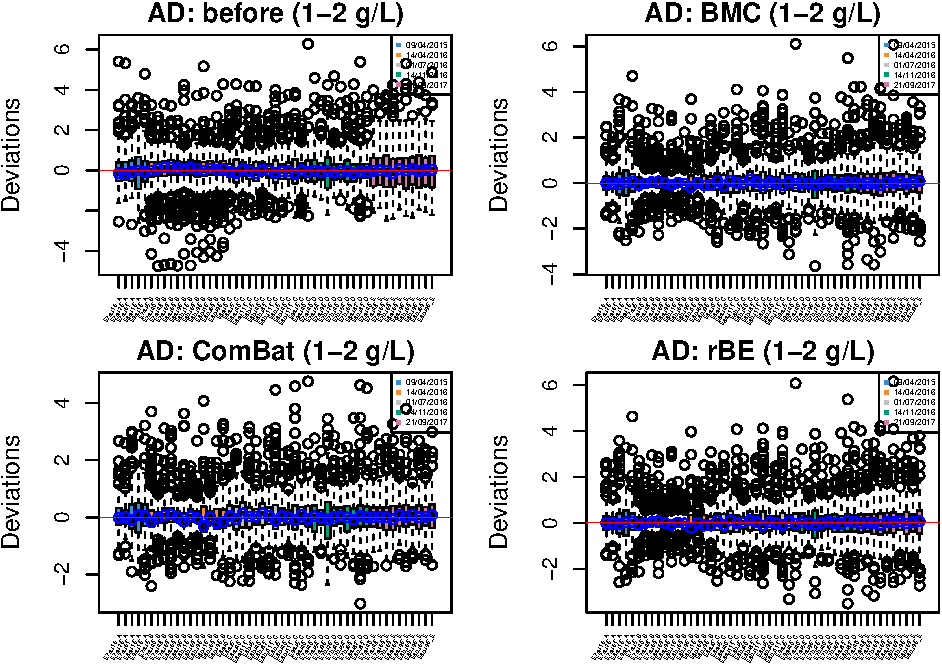
\includegraphics{vignette_files/figure-latex/unnamed-chunk-53-1.pdf}

\begin{Shaded}
\begin{Highlighting}[]
\KeywordTok{par}\NormalTok{(}\DataTypeTok{mfrow =} \KeywordTok{c}\NormalTok{(}\DecValTok{1}\NormalTok{,}\DecValTok{1}\NormalTok{))}
\end{Highlighting}
\end{Shaded}

\begin{Shaded}
\begin{Highlighting}[]
\KeywordTok{par}\NormalTok{(}\DataTypeTok{mfrow =} \KeywordTok{c}\NormalTok{(}\DecValTok{2}\NormalTok{,}\DecValTok{3}\NormalTok{), }\DataTypeTok{mai=}\KeywordTok{c}\NormalTok{(}\FloatTok{0.4}\NormalTok{,}\FloatTok{0.6}\NormalTok{,}\FloatTok{0.3}\NormalTok{,}\FloatTok{0.1}\NormalTok{))}

\KeywordTok{RleMicroRna2}\NormalTok{(}\DataTypeTok{object =} \KeywordTok{t}\NormalTok{(sponge.before_e),}\DataTypeTok{batch =}\NormalTok{ sponge.batch_e,}\DataTypeTok{maintitle =} \StringTok{'Sponge: before (ectosome)'}\NormalTok{,}\DataTypeTok{title.cex =} \DecValTok{1}\NormalTok{)}

\KeywordTok{RleMicroRna2}\NormalTok{(}\DataTypeTok{object =} \KeywordTok{t}\NormalTok{(sponge.bmc_e), }\DataTypeTok{batch =}\NormalTok{ sponge.batch_e,}\DataTypeTok{maintitle =} \StringTok{'Sponge: BMC (ectosome)'}\NormalTok{,}\DataTypeTok{title.cex =} \DecValTok{1}\NormalTok{)}

\KeywordTok{RleMicroRna2}\NormalTok{(}\DataTypeTok{object =} \KeywordTok{t}\NormalTok{(sponge.combat_e),}\DataTypeTok{batch =}\NormalTok{ sponge.batch_e,}\DataTypeTok{maintitle =} \StringTok{'Sponge: ComBat (ectosome)'}\NormalTok{,}\DataTypeTok{title.cex =} \DecValTok{1}\NormalTok{)}

\KeywordTok{RleMicroRna2}\NormalTok{(}\DataTypeTok{object =} \KeywordTok{t}\NormalTok{(sponge.limma_e),}\DataTypeTok{batch =}\NormalTok{ sponge.batch_e,}\DataTypeTok{maintitle =} \StringTok{'Sponge: rBE (ectosome)'}\NormalTok{,}\DataTypeTok{title.cex =} \DecValTok{1}\NormalTok{)}

\KeywordTok{RleMicroRna2}\NormalTok{(}\DataTypeTok{object =} \KeywordTok{t}\NormalTok{(sponge.percentile_e),}\DataTypeTok{batch =}\NormalTok{ sponge.batch_e,}\DataTypeTok{maintitle =} \StringTok{'Sponge: PN (ectosome)'}\NormalTok{,}\DataTypeTok{title.cex =} \DecValTok{1}\NormalTok{)}

\KeywordTok{RleMicroRna2}\NormalTok{(}\DataTypeTok{object =} \KeywordTok{t}\NormalTok{(sponge.svd_e),}\DataTypeTok{batch =}\NormalTok{ sponge.batch_e,}\DataTypeTok{maintitle =} \StringTok{'Sponge: SVD (ectosome)'}\NormalTok{,}\DataTypeTok{title.cex =} \DecValTok{1}\NormalTok{)}
\end{Highlighting}
\end{Shaded}

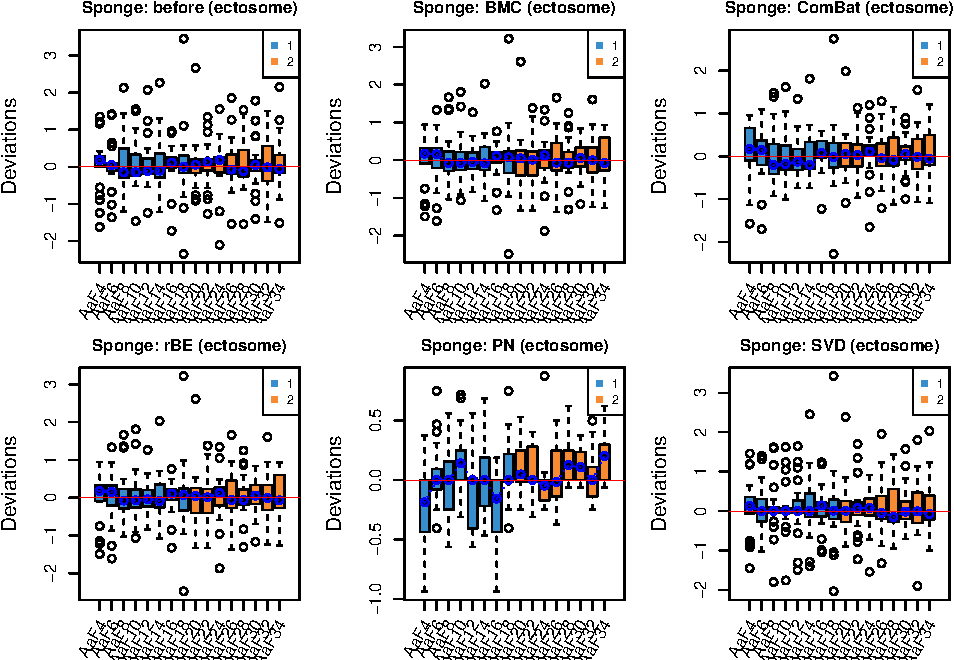
\includegraphics{vignette_files/figure-latex/unnamed-chunk-54-1.pdf}

\begin{Shaded}
\begin{Highlighting}[]
\KeywordTok{par}\NormalTok{(}\DataTypeTok{mfrow =} \KeywordTok{c}\NormalTok{(}\DecValTok{1}\NormalTok{,}\DecValTok{1}\NormalTok{))}
\end{Highlighting}
\end{Shaded}

\begin{Shaded}
\begin{Highlighting}[]
\NormalTok{################}
\CommentTok{# ad data}
\CommentTok{# before}

\NormalTok{###### BMC}
\NormalTok{ad.bmc_}\DecValTok{05}\NormalTok{ =}\StringTok{ }\NormalTok{ad.bmc[ad.trt }\OperatorTok{==}\StringTok{ '0-0.5'}\NormalTok{,]}
\NormalTok{ad.bmc_}\DecValTok{2}\NormalTok{ =}\StringTok{ }\NormalTok{ad.bmc[ad.trt }\OperatorTok{==}\StringTok{ '1-2'}\NormalTok{,]}

\NormalTok{###### ComBat}
\NormalTok{ad.combat_}\DecValTok{05}\NormalTok{ =}\StringTok{ }\NormalTok{ad.combat[ad.trt }\OperatorTok{==}\StringTok{ '0-0.5'}\NormalTok{,]}
\NormalTok{ad.combat_}\DecValTok{2}\NormalTok{ =}\StringTok{ }\NormalTok{ad.combat[ad.trt }\OperatorTok{==}\StringTok{ '1-2'}\NormalTok{,]}

\NormalTok{###### rBE}
\NormalTok{ad.limma_}\DecValTok{05}\NormalTok{ =}\StringTok{ }\NormalTok{ad.limma[ad.trt }\OperatorTok{==}\StringTok{ '0-0.5'}\NormalTok{,]}
\NormalTok{ad.limma_}\DecValTok{2}\NormalTok{ =}\StringTok{ }\NormalTok{ad.limma[ad.trt }\OperatorTok{==}\StringTok{ '1-2'}\NormalTok{,]}

\NormalTok{###### PN}
\NormalTok{ad.percentile_}\DecValTok{05}\NormalTok{ =}\StringTok{ }\NormalTok{ad.percentile[ad.trt }\OperatorTok{==}\StringTok{ '0-0.5'}\NormalTok{,]}
\NormalTok{ad.percentile_}\DecValTok{2}\NormalTok{ =}\StringTok{ }\NormalTok{ad.percentile[ad.trt }\OperatorTok{==}\StringTok{ '1-2'}\NormalTok{,]}

\NormalTok{###### SVD}
\NormalTok{ad.svd_}\DecValTok{05}\NormalTok{ =}\StringTok{ }\NormalTok{ad.svd[ad.trt }\OperatorTok{==}\StringTok{ '0-0.5'}\NormalTok{,]}
\NormalTok{ad.svd_}\DecValTok{2}\NormalTok{ =}\StringTok{ }\NormalTok{ad.svd[ad.trt }\OperatorTok{==}\StringTok{ '1-2'}\NormalTok{,]}

\NormalTok{###### RUVIII}
\NormalTok{ad.ruv_}\DecValTok{05}\NormalTok{ =}\StringTok{ }\NormalTok{ad.ruv[ad.trt }\OperatorTok{==}\StringTok{ '0-0.5'}\NormalTok{,]}
\NormalTok{ad.ruv_}\DecValTok{2}\NormalTok{ =}\StringTok{ }\NormalTok{ad.ruv[ad.trt }\OperatorTok{==}\StringTok{ '1-2'}\NormalTok{,]}
\end{Highlighting}
\end{Shaded}

\begin{Shaded}
\begin{Highlighting}[]
\KeywordTok{par}\NormalTok{(}\DataTypeTok{mfrow=}\KeywordTok{c}\NormalTok{(}\DecValTok{2}\NormalTok{,}\DecValTok{2}\NormalTok{), }\DataTypeTok{mai=}\KeywordTok{c}\NormalTok{(}\FloatTok{0.5}\NormalTok{,}\FloatTok{0.8}\NormalTok{,}\FloatTok{0.3}\NormalTok{,}\FloatTok{0.1}\NormalTok{))}

\KeywordTok{RleMicroRna2}\NormalTok{(}\DataTypeTok{object =} \KeywordTok{t}\NormalTok{(ad.before_}\DecValTok{05}\NormalTok{),}\DataTypeTok{batch =}\NormalTok{ ad.batch_}\DecValTok{05}\NormalTok{,}\DataTypeTok{maintitle =} \StringTok{'AD: before (0-0.5 g/L)'}\NormalTok{,}\DataTypeTok{legend.cex =} \FloatTok{0.4}\NormalTok{, }\DataTypeTok{cex.xaxis =} \FloatTok{0.5}\NormalTok{)}

\KeywordTok{RleMicroRna2}\NormalTok{(}\DataTypeTok{object =} \KeywordTok{t}\NormalTok{(ad.bmc_}\DecValTok{05}\NormalTok{),}\DataTypeTok{batch =}\NormalTok{ ad.batch_}\DecValTok{05}\NormalTok{,}\DataTypeTok{maintitle =} \StringTok{'AD: BMC (0-0.5 g/L)'}\NormalTok{,}\DataTypeTok{legend.cex =} \FloatTok{0.4}\NormalTok{, }\DataTypeTok{cex.xaxis =} \FloatTok{0.5}\NormalTok{)}

\KeywordTok{RleMicroRna2}\NormalTok{(}\DataTypeTok{object =} \KeywordTok{t}\NormalTok{(ad.combat_}\DecValTok{05}\NormalTok{),}\DataTypeTok{batch =}\NormalTok{ ad.batch_}\DecValTok{05}\NormalTok{,}\DataTypeTok{maintitle =} \StringTok{'AD: ComBat (0-0.5 g/L)'}\NormalTok{,}\DataTypeTok{legend.cex =} \FloatTok{0.4}\NormalTok{, }\DataTypeTok{cex.xaxis =} \FloatTok{0.5}\NormalTok{)}

\KeywordTok{RleMicroRna2}\NormalTok{(}\DataTypeTok{object =} \KeywordTok{t}\NormalTok{(ad.limma_}\DecValTok{05}\NormalTok{),}\DataTypeTok{batch =}\NormalTok{ ad.batch_}\DecValTok{05}\NormalTok{,}\DataTypeTok{maintitle =} \StringTok{'AD: rBE (0-0.5 g/L)'}\NormalTok{,}\DataTypeTok{legend.cex =} \FloatTok{0.4}\NormalTok{, }\DataTypeTok{cex.xaxis =} \FloatTok{0.5}\NormalTok{)}
\end{Highlighting}
\end{Shaded}

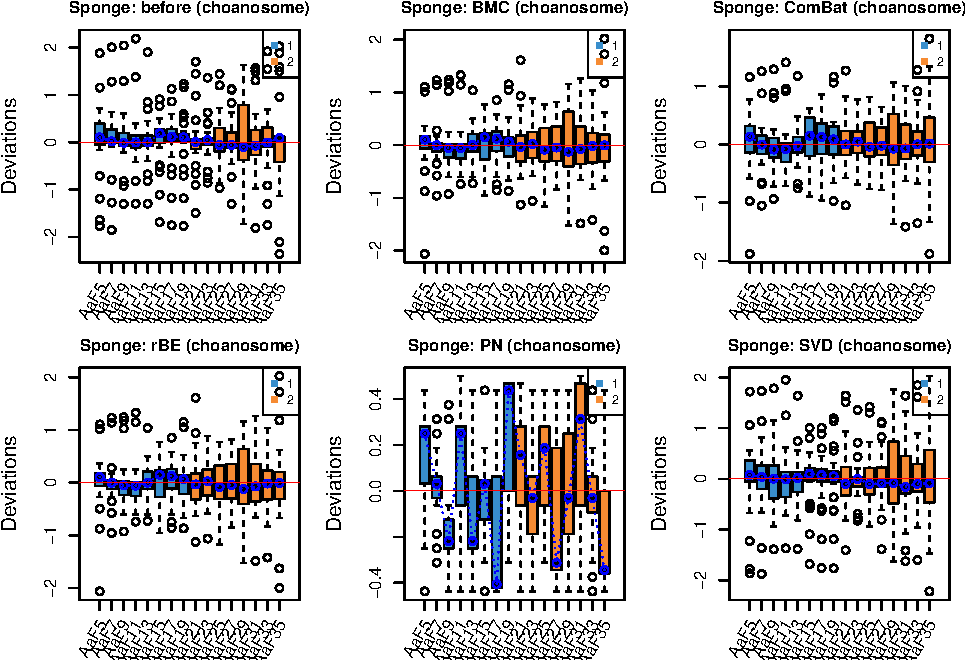
\includegraphics{vignette_files/figure-latex/unnamed-chunk-56-1.pdf}

\begin{Shaded}
\begin{Highlighting}[]
\KeywordTok{RleMicroRna2}\NormalTok{(}\DataTypeTok{object =} \KeywordTok{t}\NormalTok{(ad.percentile_}\DecValTok{05}\NormalTok{),}\DataTypeTok{batch =}\NormalTok{ ad.batch_}\DecValTok{05}\NormalTok{,}\DataTypeTok{maintitle =} \StringTok{'AD: PN (0-0.5 g/L)'}\NormalTok{,}\DataTypeTok{legend.cex =} \FloatTok{0.4}\NormalTok{, }\DataTypeTok{cex.xaxis =} \FloatTok{0.5}\NormalTok{)}

\KeywordTok{RleMicroRna2}\NormalTok{(}\DataTypeTok{object =} \KeywordTok{t}\NormalTok{(ad.svd_}\DecValTok{05}\NormalTok{),}\DataTypeTok{batch =}\NormalTok{ ad.batch_}\DecValTok{05}\NormalTok{,}\DataTypeTok{maintitle =} \StringTok{'AD: SVD (0-0.5 g/L)'}\NormalTok{,}\DataTypeTok{legend.cex =} \FloatTok{0.4}\NormalTok{, }\DataTypeTok{cex.xaxis =} \FloatTok{0.5}\NormalTok{)}

\KeywordTok{RleMicroRna2}\NormalTok{(}\DataTypeTok{object =} \KeywordTok{t}\NormalTok{(ad.ruv_}\DecValTok{05}\NormalTok{),}\DataTypeTok{batch =}\NormalTok{ ad.batch_}\DecValTok{05}\NormalTok{,}\DataTypeTok{maintitle =} \StringTok{'AD: RUVIII (0-0.5 g/L)'}\NormalTok{,}\DataTypeTok{legend.cex =} \FloatTok{0.4}\NormalTok{, }\DataTypeTok{cex.xaxis =} \FloatTok{0.5}\NormalTok{)}

\KeywordTok{par}\NormalTok{(}\DataTypeTok{mfrow =} \KeywordTok{c}\NormalTok{(}\DecValTok{1}\NormalTok{,}\DecValTok{1}\NormalTok{))}
\end{Highlighting}
\end{Shaded}

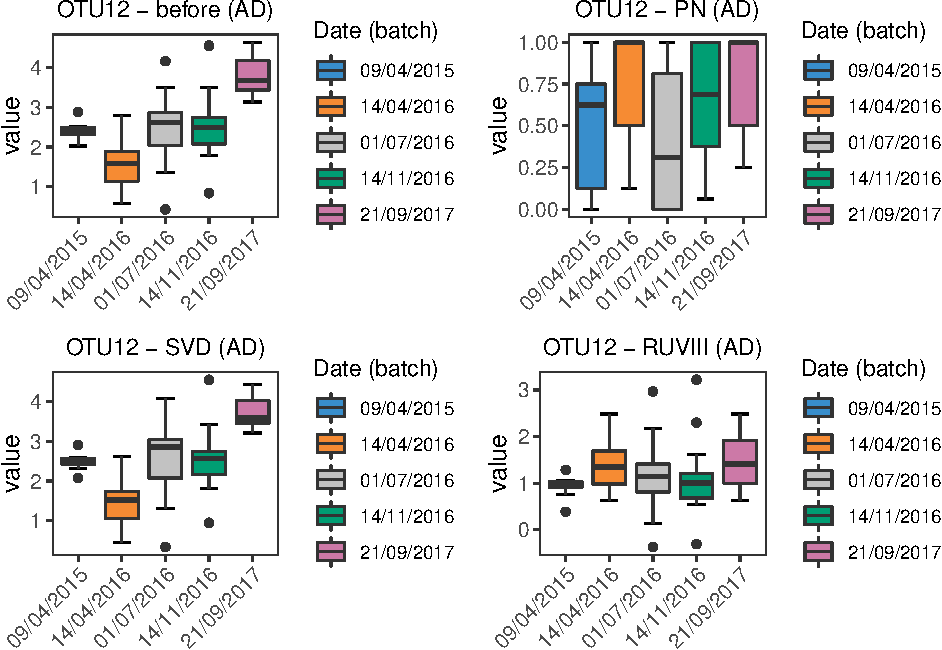
\includegraphics{vignette_files/figure-latex/unnamed-chunk-56-2.pdf}

\begin{Shaded}
\begin{Highlighting}[]
\KeywordTok{par}\NormalTok{(}\DataTypeTok{mfrow=}\KeywordTok{c}\NormalTok{(}\DecValTok{2}\NormalTok{,}\DecValTok{2}\NormalTok{), }\DataTypeTok{mai=}\KeywordTok{c}\NormalTok{(}\FloatTok{0.35}\NormalTok{,}\FloatTok{0.8}\NormalTok{,}\FloatTok{0.3}\NormalTok{,}\FloatTok{0.1}\NormalTok{))}

\KeywordTok{RleMicroRna2}\NormalTok{(}\DataTypeTok{object =} \KeywordTok{t}\NormalTok{(ad.before_}\DecValTok{2}\NormalTok{),}\DataTypeTok{batch =}\NormalTok{ ad.batch_}\DecValTok{2}\NormalTok{,}\DataTypeTok{maintitle =} \StringTok{'AD: before (1-2 g/L)'}\NormalTok{,}\DataTypeTok{legend.cex =} \FloatTok{0.4}\NormalTok{, }\DataTypeTok{cex.xaxis =} \FloatTok{0.3}\NormalTok{)}

\KeywordTok{RleMicroRna2}\NormalTok{(}\DataTypeTok{object =} \KeywordTok{t}\NormalTok{(ad.bmc_}\DecValTok{2}\NormalTok{),}\DataTypeTok{batch =}\NormalTok{ ad.batch_}\DecValTok{2}\NormalTok{,}\DataTypeTok{maintitle =} \StringTok{'AD: BMC (1-2 g/L)'}\NormalTok{,}\DataTypeTok{legend.cex =} \FloatTok{0.4}\NormalTok{, }\DataTypeTok{cex.xaxis =} \FloatTok{0.3}\NormalTok{)}

\KeywordTok{RleMicroRna2}\NormalTok{(}\DataTypeTok{object =} \KeywordTok{t}\NormalTok{(ad.combat_}\DecValTok{2}\NormalTok{),}\DataTypeTok{batch =}\NormalTok{ ad.batch_}\DecValTok{2}\NormalTok{,}\DataTypeTok{maintitle =} \StringTok{'AD: ComBat (1-2 g/L)'}\NormalTok{,}\DataTypeTok{legend.cex =} \FloatTok{0.4}\NormalTok{, }\DataTypeTok{cex.xaxis =} \FloatTok{0.3}\NormalTok{)}

\KeywordTok{RleMicroRna2}\NormalTok{(}\DataTypeTok{object =} \KeywordTok{t}\NormalTok{(ad.limma_}\DecValTok{2}\NormalTok{),}\DataTypeTok{batch =}\NormalTok{ ad.batch_}\DecValTok{2}\NormalTok{,}\DataTypeTok{maintitle =} \StringTok{'AD: rBE (1-2 g/L)'}\NormalTok{,}\DataTypeTok{legend.cex =} \FloatTok{0.4}\NormalTok{, }\DataTypeTok{cex.xaxis =} \FloatTok{0.3}\NormalTok{)}
\end{Highlighting}
\end{Shaded}

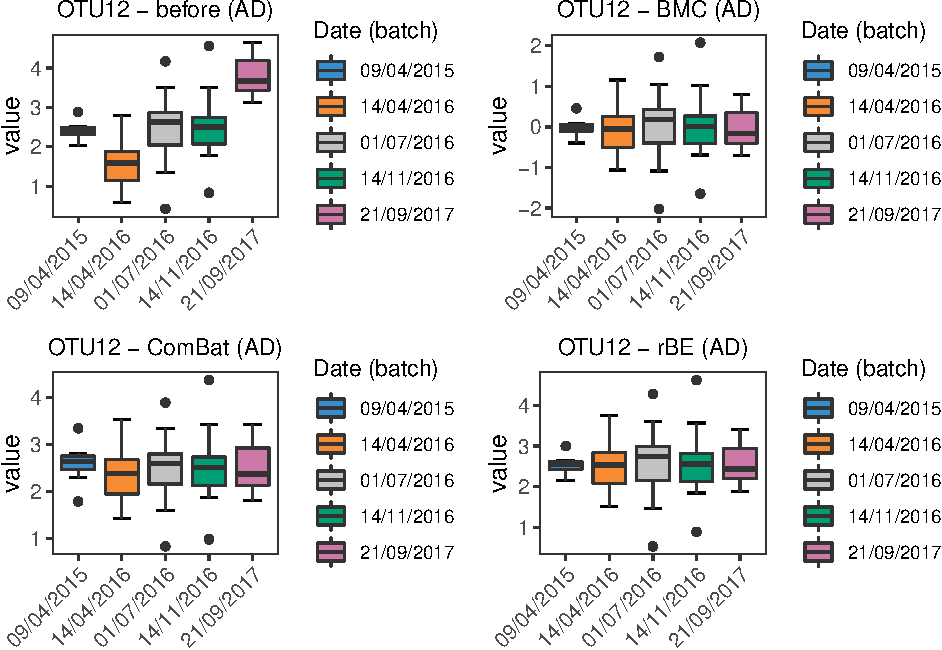
\includegraphics{vignette_files/figure-latex/unnamed-chunk-57-1.pdf}

\begin{Shaded}
\begin{Highlighting}[]
\KeywordTok{RleMicroRna2}\NormalTok{(}\DataTypeTok{object =} \KeywordTok{t}\NormalTok{(ad.percentile_}\DecValTok{2}\NormalTok{),}\DataTypeTok{batch =}\NormalTok{ ad.batch_}\DecValTok{2}\NormalTok{,}\DataTypeTok{maintitle =} \StringTok{'AD: PN (1-2 g/L)'}\NormalTok{,}\DataTypeTok{legend.cex =} \FloatTok{0.4}\NormalTok{, }\DataTypeTok{cex.xaxis =} \FloatTok{0.3}\NormalTok{)}

\KeywordTok{RleMicroRna2}\NormalTok{(}\DataTypeTok{object =} \KeywordTok{t}\NormalTok{(ad.svd_}\DecValTok{2}\NormalTok{),}\DataTypeTok{batch =}\NormalTok{ ad.batch_}\DecValTok{2}\NormalTok{,}\DataTypeTok{maintitle =} \StringTok{'AD: SVD (1-2 g/L)'}\NormalTok{,}\DataTypeTok{legend.cex =} \FloatTok{0.4}\NormalTok{, }\DataTypeTok{cex.xaxis =} \FloatTok{0.3}\NormalTok{)}

\KeywordTok{RleMicroRna2}\NormalTok{(}\DataTypeTok{object =} \KeywordTok{t}\NormalTok{(ad.ruv_}\DecValTok{2}\NormalTok{),}\DataTypeTok{batch =}\NormalTok{ ad.batch_}\DecValTok{2}\NormalTok{,}\DataTypeTok{maintitle =} \StringTok{'AD: RUVIII (1-2 g/L)'}\NormalTok{,}\DataTypeTok{legend.cex =} \FloatTok{0.4}\NormalTok{, }\DataTypeTok{cex.xaxis =} \FloatTok{0.3}\NormalTok{)}

\KeywordTok{par}\NormalTok{(}\DataTypeTok{mfrow =} \KeywordTok{c}\NormalTok{(}\DecValTok{1}\NormalTok{,}\DecValTok{1}\NormalTok{))}
\end{Highlighting}
\end{Shaded}

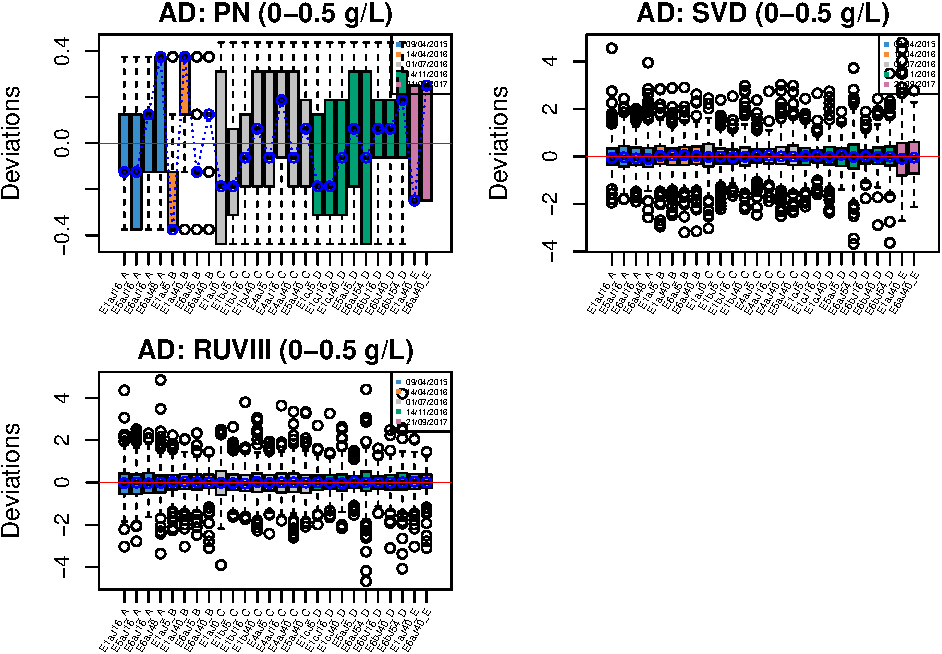
\includegraphics{vignette_files/figure-latex/unnamed-chunk-57-2.pdf}

\subsection{Heatmap}\label{heatmap-1}

\begin{Shaded}
\begin{Highlighting}[]
\CommentTok{# Sponge data}
\CommentTok{# before }
\NormalTok{sponge.tss.clr.scale =}\StringTok{ }\KeywordTok{scale}\NormalTok{(sponge.tss.clr,}\DataTypeTok{center =}\NormalTok{ T, }\DataTypeTok{scale =}\NormalTok{ T) }\CommentTok{# scale on OTUs}
\NormalTok{sponge.tss.clr.scale =}\StringTok{ }\KeywordTok{scale}\NormalTok{(}\KeywordTok{t}\NormalTok{(sponge.tss.clr.scale), }\DataTypeTok{center =}\NormalTok{ T, }\DataTypeTok{scale =}\NormalTok{ T) }\CommentTok{# scale on samples}

\NormalTok{anno_col.sponge =}\StringTok{ }\KeywordTok{data.frame}\NormalTok{(}\DataTypeTok{Batch =}\NormalTok{ sponge.batch, }\DataTypeTok{Tissue =}\NormalTok{ sponge.trt)}
\NormalTok{anno_metabo_colors.sponge =}\StringTok{ }\KeywordTok{list}\NormalTok{(}\DataTypeTok{Batch =} \KeywordTok{c}\NormalTok{(}\StringTok{'1'}\NormalTok{=}\StringTok{"#388ECC"}\NormalTok{,}\StringTok{'2'}\NormalTok{=}\StringTok{"#F68B33"}\NormalTok{),}\DataTypeTok{Tissue =} \KeywordTok{c}\NormalTok{(}\DataTypeTok{C=}\StringTok{"#F0E442"}\NormalTok{,}\DataTypeTok{E=}\StringTok{"#D55E00"}\NormalTok{))}


\KeywordTok{pheatmap}\NormalTok{(sponge.tss.clr.scale, }
         \DataTypeTok{scale =} \StringTok{'none'}\NormalTok{, }
         \DataTypeTok{cluster_rows =}\NormalTok{ F, }
         \DataTypeTok{cluster_cols =}\NormalTok{ T, }
         \DataTypeTok{fontsize_row=}\DecValTok{5}\NormalTok{, }\DataTypeTok{fontsize_col=}\DecValTok{8}\NormalTok{,}
         \DataTypeTok{fontsize =} \DecValTok{8}\NormalTok{,}
         \DataTypeTok{clustering_distance_rows =} \StringTok{"euclidean"}\NormalTok{,}
         \DataTypeTok{clustering_method =} \StringTok{"ward.D"}\NormalTok{,}
         \DataTypeTok{treeheight_row =} \DecValTok{30}\NormalTok{,}
         \DataTypeTok{annotation_col =}\NormalTok{ anno_col.sponge,}
         \DataTypeTok{annotation_colors=}\NormalTok{anno_metabo_colors.sponge,}
         \DataTypeTok{border_color =} \StringTok{'NA'}\NormalTok{,}
         \DataTypeTok{main =} \StringTok{'Sponge data - before'}\NormalTok{)}
\end{Highlighting}
\end{Shaded}

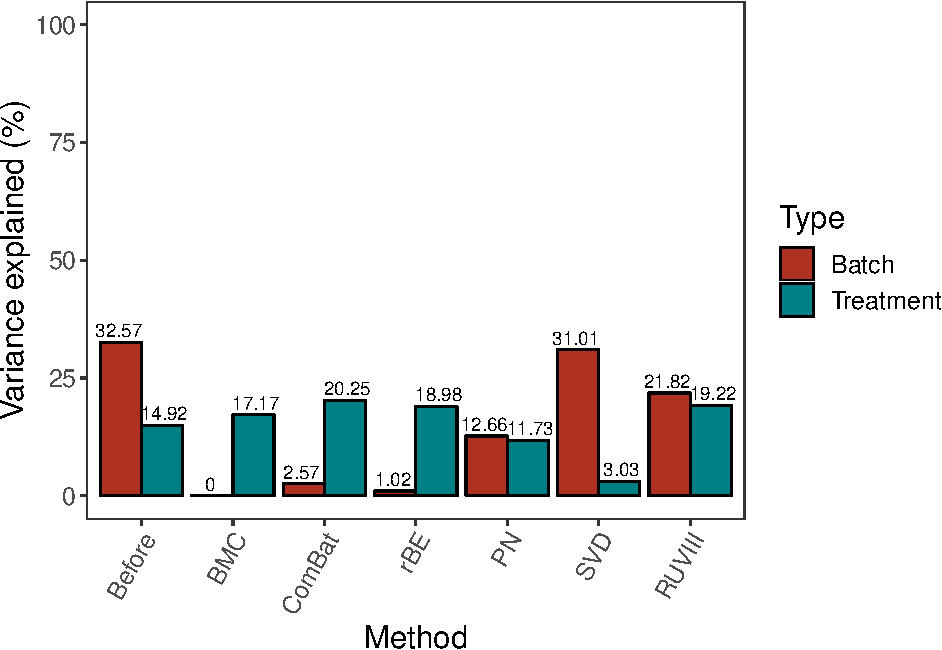
\includegraphics{vignette_files/figure-latex/unnamed-chunk-58-1.pdf}

\begin{Shaded}
\begin{Highlighting}[]
\CommentTok{# BMC }
\NormalTok{sponge.bmc.scale =}\StringTok{ }\KeywordTok{scale}\NormalTok{(sponge.bmc,}\DataTypeTok{center =}\NormalTok{ T, }\DataTypeTok{scale =}\NormalTok{ T) }\CommentTok{# scale on OTUs}
\NormalTok{sponge.bmc.scale =}\StringTok{ }\KeywordTok{scale}\NormalTok{(}\KeywordTok{t}\NormalTok{(sponge.bmc.scale), }\DataTypeTok{center =}\NormalTok{ T, }\DataTypeTok{scale =}\NormalTok{ T) }\CommentTok{# scale on samples}

\KeywordTok{pheatmap}\NormalTok{(sponge.bmc.scale, }
         \DataTypeTok{scale =} \StringTok{'none'}\NormalTok{, }
         \DataTypeTok{cluster_rows =}\NormalTok{ F, }
         \DataTypeTok{cluster_cols =}\NormalTok{ T, }
         \DataTypeTok{fontsize_row=}\DecValTok{5}\NormalTok{, }\DataTypeTok{fontsize_col=}\DecValTok{8}\NormalTok{,}
         \DataTypeTok{fontsize =} \DecValTok{8}\NormalTok{,}
         \DataTypeTok{clustering_distance_rows =} \StringTok{"euclidean"}\NormalTok{,}
         \DataTypeTok{clustering_method =} \StringTok{"ward.D"}\NormalTok{,}
         \DataTypeTok{treeheight_row =} \DecValTok{30}\NormalTok{,}
         \DataTypeTok{annotation_col =}\NormalTok{ anno_col.sponge,}
         \DataTypeTok{annotation_colors=}\NormalTok{anno_metabo_colors.sponge,}
         \DataTypeTok{border_color =} \StringTok{'NA'}\NormalTok{,}
         \DataTypeTok{main =} \StringTok{'Sponge data - BMC'}\NormalTok{)}
\end{Highlighting}
\end{Shaded}

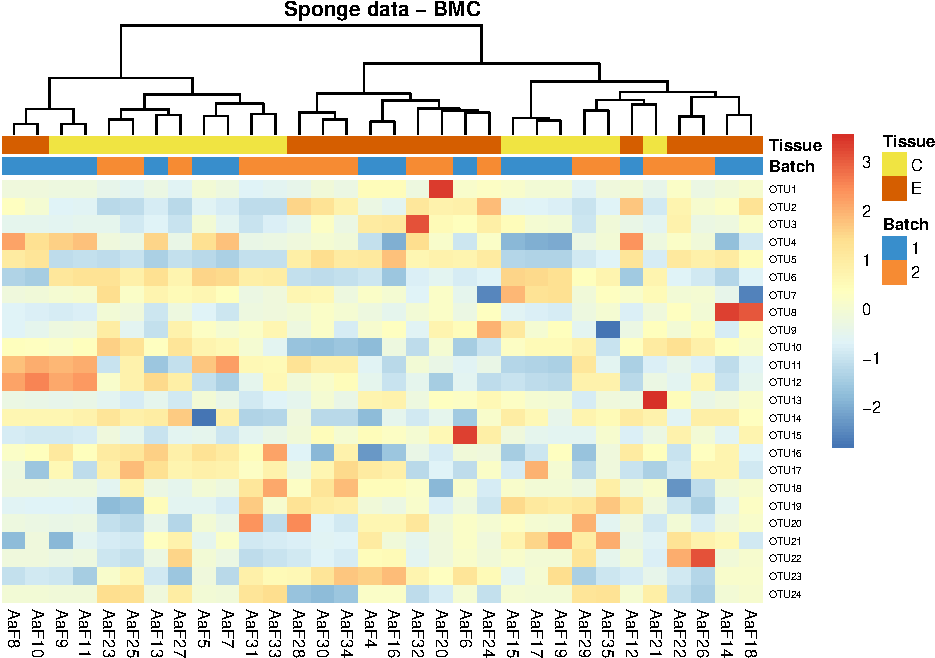
\includegraphics{vignette_files/figure-latex/unnamed-chunk-58-2.pdf}

\begin{Shaded}
\begin{Highlighting}[]
\CommentTok{# ComBat }
\NormalTok{sponge.combat.scale =}\StringTok{ }\KeywordTok{scale}\NormalTok{(sponge.combat,}\DataTypeTok{center =}\NormalTok{ T, }\DataTypeTok{scale =}\NormalTok{ T) }\CommentTok{# scale on OTUs}
\NormalTok{sponge.combat.scale =}\StringTok{ }\KeywordTok{scale}\NormalTok{(}\KeywordTok{t}\NormalTok{(sponge.combat.scale), }\DataTypeTok{center =}\NormalTok{ T, }\DataTypeTok{scale =}\NormalTok{ T) }\CommentTok{# scale on samples}

\KeywordTok{pheatmap}\NormalTok{(sponge.combat.scale, }
         \DataTypeTok{scale =} \StringTok{'none'}\NormalTok{, }
         \DataTypeTok{cluster_rows =}\NormalTok{ F, }
         \DataTypeTok{cluster_cols =}\NormalTok{ T, }
         \DataTypeTok{fontsize_row=}\DecValTok{5}\NormalTok{, }\DataTypeTok{fontsize_col=}\DecValTok{8}\NormalTok{,}
         \DataTypeTok{fontsize =} \DecValTok{8}\NormalTok{,}
         \DataTypeTok{clustering_distance_rows =} \StringTok{"euclidean"}\NormalTok{,}
         \DataTypeTok{clustering_method =} \StringTok{"ward.D"}\NormalTok{,}
         \DataTypeTok{treeheight_row =} \DecValTok{30}\NormalTok{,}
         \DataTypeTok{annotation_col =}\NormalTok{ anno_col.sponge,}
         \DataTypeTok{annotation_colors=}\NormalTok{anno_metabo_colors.sponge,}
         \DataTypeTok{border_color =} \StringTok{'NA'}\NormalTok{,}
         \DataTypeTok{main =} \StringTok{'Sponge data - ComBat'}\NormalTok{)}
\end{Highlighting}
\end{Shaded}

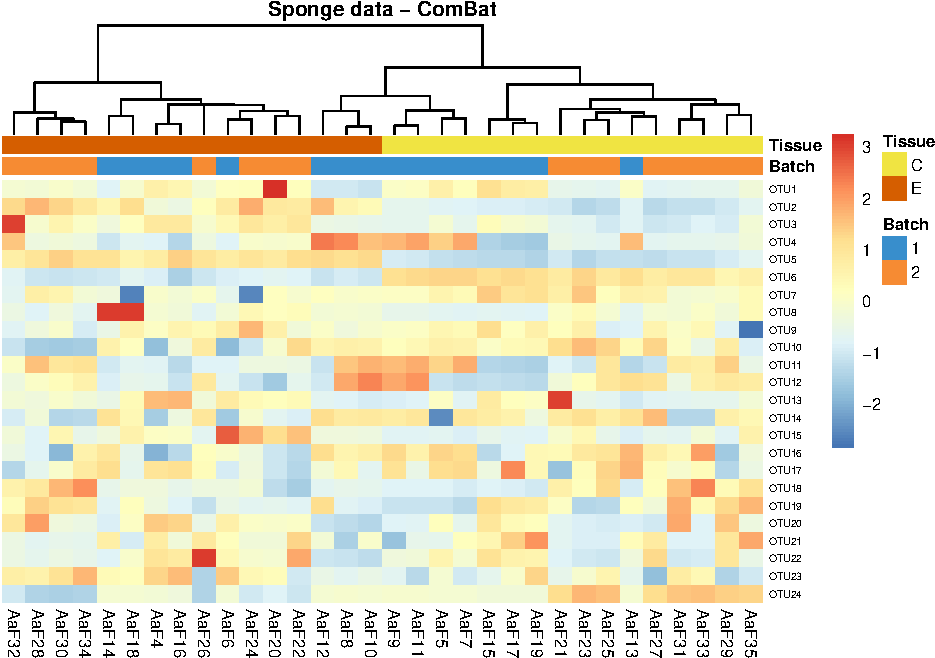
\includegraphics{vignette_files/figure-latex/unnamed-chunk-58-3.pdf}

\begin{Shaded}
\begin{Highlighting}[]
\CommentTok{# removeBatchEffect}
\NormalTok{sponge.limma.scale =}\StringTok{ }\KeywordTok{scale}\NormalTok{(sponge.limma,}\DataTypeTok{center =}\NormalTok{ T, }\DataTypeTok{scale =}\NormalTok{ T) }\CommentTok{# scale on OTUs}
\NormalTok{sponge.limma.scale =}\StringTok{ }\KeywordTok{scale}\NormalTok{(}\KeywordTok{t}\NormalTok{(sponge.limma.scale), }\DataTypeTok{center =}\NormalTok{ T, }\DataTypeTok{scale =}\NormalTok{ T) }\CommentTok{# scale on samples}

\KeywordTok{pheatmap}\NormalTok{(sponge.limma.scale, }
         \DataTypeTok{scale =} \StringTok{'none'}\NormalTok{, }
         \DataTypeTok{cluster_rows =}\NormalTok{ F, }
         \DataTypeTok{cluster_cols =}\NormalTok{ T, }
         \DataTypeTok{fontsize_row=}\DecValTok{5}\NormalTok{, }\DataTypeTok{fontsize_col=}\DecValTok{8}\NormalTok{,}
         \DataTypeTok{fontsize =} \DecValTok{8}\NormalTok{,}
         \DataTypeTok{clustering_distance_rows =} \StringTok{"euclidean"}\NormalTok{,}
         \DataTypeTok{clustering_method =} \StringTok{"ward.D"}\NormalTok{,}
         \DataTypeTok{treeheight_row =} \DecValTok{30}\NormalTok{,}
         \DataTypeTok{annotation_col =}\NormalTok{ anno_col.sponge,}
         \DataTypeTok{annotation_colors=}\NormalTok{anno_metabo_colors.sponge,}
         \DataTypeTok{border_color =} \StringTok{'NA'}\NormalTok{,}
         \DataTypeTok{main =} \StringTok{'Sponge data - removeBatchEffect'}\NormalTok{)}
\end{Highlighting}
\end{Shaded}

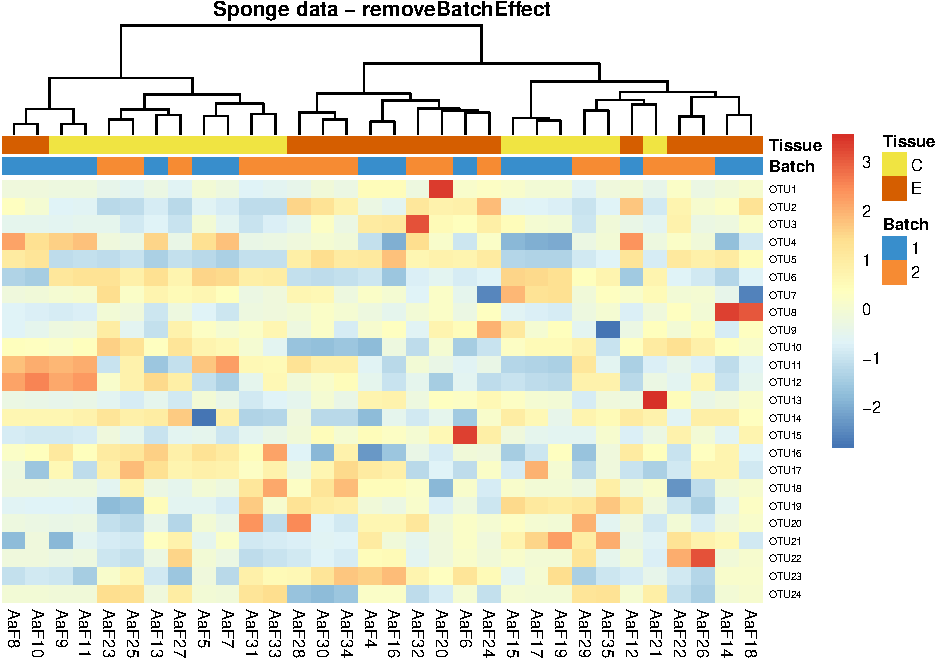
\includegraphics{vignette_files/figure-latex/unnamed-chunk-58-4.pdf}

\begin{Shaded}
\begin{Highlighting}[]
\CommentTok{# percentile normalisation}
\NormalTok{sponge.percentile.scale =}\StringTok{ }\KeywordTok{scale}\NormalTok{(sponge.percentile,}\DataTypeTok{center =}\NormalTok{ T, }\DataTypeTok{scale =}\NormalTok{ T) }\CommentTok{# scale on OTUs}
\NormalTok{sponge.percentile.scale =}\StringTok{ }\KeywordTok{scale}\NormalTok{(}\KeywordTok{t}\NormalTok{(sponge.percentile.scale), }\DataTypeTok{center =}\NormalTok{ T, }\DataTypeTok{scale =}\NormalTok{ T) }\CommentTok{# scale on samples}

\KeywordTok{pheatmap}\NormalTok{(sponge.percentile.scale, }
         \DataTypeTok{scale =} \StringTok{'none'}\NormalTok{, }
         \DataTypeTok{cluster_rows =}\NormalTok{ F, }
         \DataTypeTok{cluster_cols =}\NormalTok{ T, }
         \DataTypeTok{fontsize_row=}\DecValTok{5}\NormalTok{, }\DataTypeTok{fontsize_col=}\DecValTok{8}\NormalTok{,}
         \DataTypeTok{fontsize =} \DecValTok{8}\NormalTok{,}
         \DataTypeTok{clustering_distance_rows =} \StringTok{"euclidean"}\NormalTok{,}
         \DataTypeTok{clustering_method =} \StringTok{"ward.D"}\NormalTok{,}
         \DataTypeTok{treeheight_row =} \DecValTok{30}\NormalTok{,}
         \DataTypeTok{annotation_col =}\NormalTok{ anno_col.sponge,}
         \DataTypeTok{annotation_colors=}\NormalTok{anno_metabo_colors.sponge,}
         \DataTypeTok{border_color =} \StringTok{'NA'}\NormalTok{,}
         \DataTypeTok{main =} \StringTok{'Sponge data - percentile norm'}\NormalTok{)}
\end{Highlighting}
\end{Shaded}

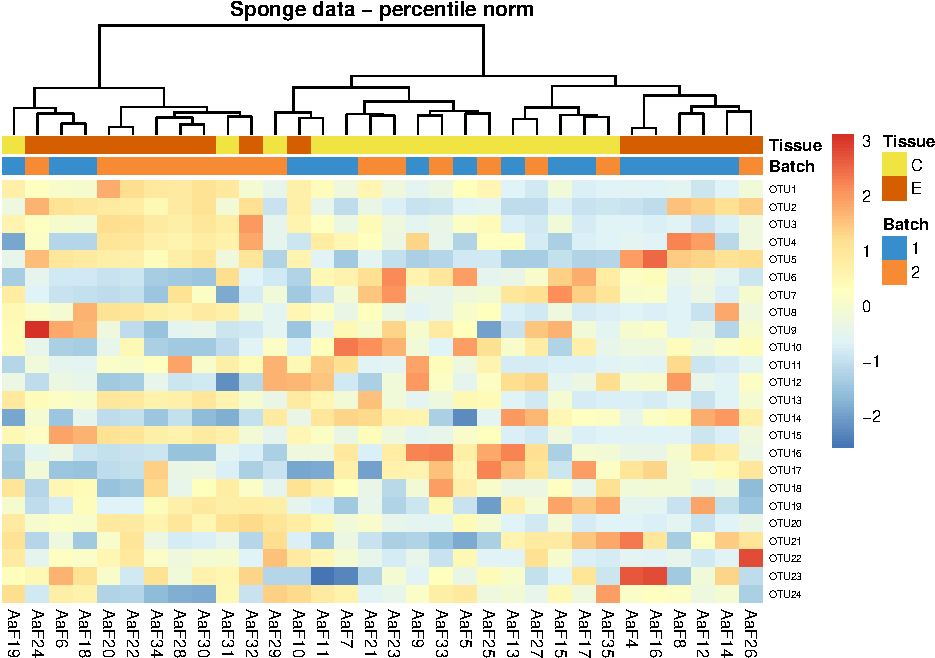
\includegraphics{vignette_files/figure-latex/unnamed-chunk-58-5.pdf}

\begin{Shaded}
\begin{Highlighting}[]
\CommentTok{# SVD}
\NormalTok{sponge.svd.scale =}\StringTok{ }\KeywordTok{scale}\NormalTok{(sponge.svd,}\DataTypeTok{center =}\NormalTok{ T, }\DataTypeTok{scale =}\NormalTok{ T) }\CommentTok{# scale on OTUs}
\NormalTok{sponge.svd.scale =}\StringTok{ }\KeywordTok{scale}\NormalTok{(}\KeywordTok{t}\NormalTok{(sponge.svd.scale), }\DataTypeTok{center =}\NormalTok{ T, }\DataTypeTok{scale =}\NormalTok{ T) }\CommentTok{# scale on samples}

\KeywordTok{pheatmap}\NormalTok{(sponge.svd.scale, }
         \DataTypeTok{scale =} \StringTok{'none'}\NormalTok{, }
         \DataTypeTok{cluster_rows =}\NormalTok{ F, }
         \DataTypeTok{cluster_cols =}\NormalTok{ T, }
         \DataTypeTok{fontsize_row=}\DecValTok{5}\NormalTok{, }\DataTypeTok{fontsize_col=}\DecValTok{8}\NormalTok{,}
         \DataTypeTok{fontsize =} \DecValTok{8}\NormalTok{,}
         \DataTypeTok{clustering_distance_rows =} \StringTok{"euclidean"}\NormalTok{,}
         \DataTypeTok{clustering_method =} \StringTok{"ward.D"}\NormalTok{,}
         \DataTypeTok{treeheight_row =} \DecValTok{30}\NormalTok{,}
         \DataTypeTok{annotation_col =}\NormalTok{ anno_col.sponge,}
         \DataTypeTok{annotation_colors=}\NormalTok{anno_metabo_colors.sponge,}
         \DataTypeTok{border_color =} \StringTok{'NA'}\NormalTok{,}
         \DataTypeTok{main =} \StringTok{'Sponge data - SVD'}\NormalTok{)}
\end{Highlighting}
\end{Shaded}

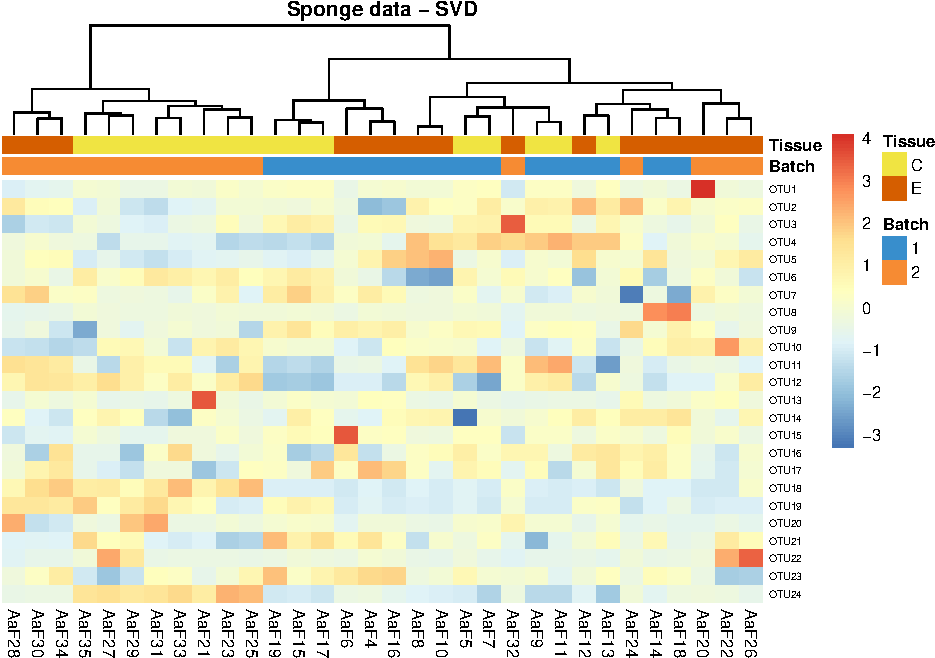
\includegraphics{vignette_files/figure-latex/unnamed-chunk-58-6.pdf}

\begin{Shaded}
\begin{Highlighting}[]
\NormalTok{#################}
\CommentTok{# AD data}
\CommentTok{# before }
\NormalTok{ad.tss.clr.scale =}\StringTok{ }\KeywordTok{scale}\NormalTok{(ad.tss.clr,}\DataTypeTok{center =}\NormalTok{ T, }\DataTypeTok{scale =}\NormalTok{ T) }\CommentTok{# scale on OTUs}
\NormalTok{ad.tss.clr.scale =}\StringTok{ }\KeywordTok{scale}\NormalTok{(}\KeywordTok{t}\NormalTok{(ad.tss.clr.scale), }\DataTypeTok{center =}\NormalTok{ T, }\DataTypeTok{scale =}\NormalTok{ T) }\CommentTok{# scale on samples}

\NormalTok{anno_col.ad =}\StringTok{ }\KeywordTok{data.frame}\NormalTok{(}\DataTypeTok{Batch =}\NormalTok{ ad.batch, }\DataTypeTok{Treatment =}\NormalTok{ ad.trt)}
\NormalTok{anno_metabo_colors.ad =}\StringTok{ }\KeywordTok{list}\NormalTok{(}\DataTypeTok{Batch =} \KeywordTok{c}\NormalTok{(}\StringTok{'09/04/2015'}\NormalTok{=}\StringTok{"#388ECC"}\NormalTok{,}\StringTok{'14/04/2016'}\NormalTok{=}\StringTok{"#F68B33"}\NormalTok{,}\StringTok{'01/07/2016'}\NormalTok{=}\StringTok{"#C2C2C2"}\NormalTok{,}\StringTok{'14/11/2016'}\NormalTok{=}\StringTok{"#009E73"}\NormalTok{,}\StringTok{'21/09/2017'}\NormalTok{=}\StringTok{"#CC79A7"}\NormalTok{), }\DataTypeTok{Treatment =} \KeywordTok{c}\NormalTok{(}\StringTok{"0-0.5"}\NormalTok{ =}\StringTok{ "#0072B2"}\NormalTok{, }\StringTok{"1-2"}\NormalTok{ =}\StringTok{ "#999999"}\NormalTok{))}


\KeywordTok{pheatmap}\NormalTok{(ad.tss.clr.scale, }
         \DataTypeTok{scale =} \StringTok{'none'}\NormalTok{, }
         \DataTypeTok{cluster_rows =}\NormalTok{ F, }
         \DataTypeTok{cluster_cols =}\NormalTok{ T, }
         \DataTypeTok{fontsize_row=}\DecValTok{4}\NormalTok{, }\DataTypeTok{fontsize_col=}\DecValTok{6}\NormalTok{,}
         \DataTypeTok{fontsize =} \DecValTok{8}\NormalTok{,}
         \DataTypeTok{clustering_distance_rows =} \StringTok{"euclidean"}\NormalTok{,}
         \DataTypeTok{clustering_method =} \StringTok{"ward.D"}\NormalTok{,}
         \DataTypeTok{treeheight_row =} \DecValTok{30}\NormalTok{,}
         \DataTypeTok{annotation_col =}\NormalTok{ anno_col.ad,}
         \DataTypeTok{annotation_colors=}\NormalTok{anno_metabo_colors.ad,}
         \DataTypeTok{border_color =} \StringTok{'NA'}\NormalTok{,}
         \DataTypeTok{main =} \StringTok{'AD data - Scaled'}\NormalTok{)}
\end{Highlighting}
\end{Shaded}

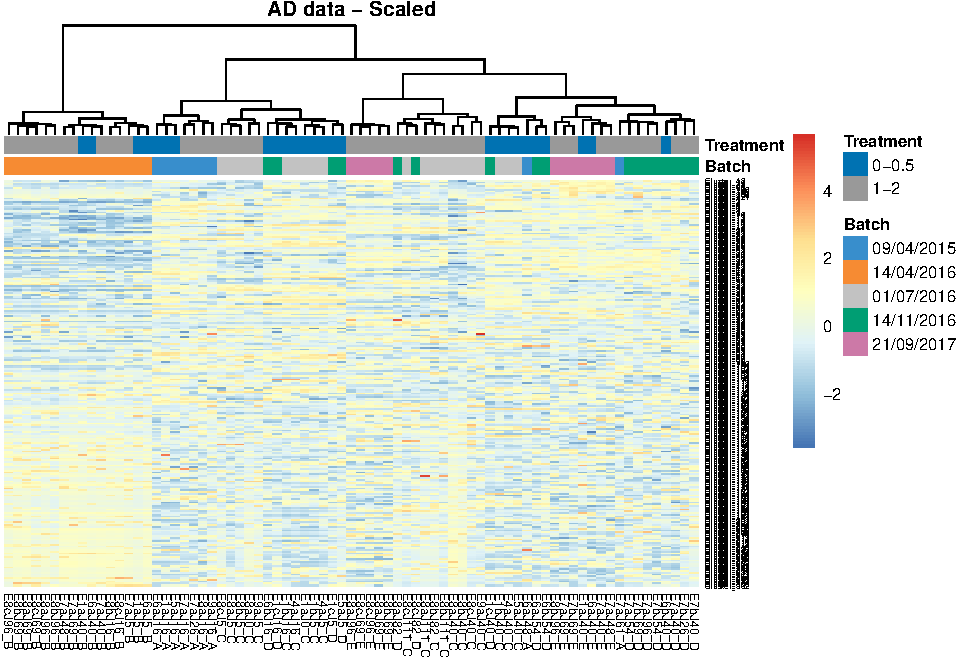
\includegraphics{vignette_files/figure-latex/unnamed-chunk-58-7.pdf}

\begin{Shaded}
\begin{Highlighting}[]
\CommentTok{# BMC}
\NormalTok{ad.bmc.scale =}\StringTok{ }\KeywordTok{scale}\NormalTok{(ad.bmc,}\DataTypeTok{center =}\NormalTok{ T, }\DataTypeTok{scale =}\NormalTok{ T) }\CommentTok{# scale on OTUs}
\NormalTok{ad.bmc.scale =}\StringTok{ }\KeywordTok{scale}\NormalTok{(}\KeywordTok{t}\NormalTok{(ad.bmc.scale), }\DataTypeTok{center =}\NormalTok{ T, }\DataTypeTok{scale =}\NormalTok{ T) }\CommentTok{# scale on samples}

\KeywordTok{pheatmap}\NormalTok{(ad.bmc.scale, }
         \DataTypeTok{scale =} \StringTok{'none'}\NormalTok{, }
         \DataTypeTok{cluster_rows =}\NormalTok{ F, }
         \DataTypeTok{cluster_cols =}\NormalTok{ T, }
         \DataTypeTok{fontsize_row=}\DecValTok{4}\NormalTok{, }\DataTypeTok{fontsize_col=}\DecValTok{6}\NormalTok{,}
         \DataTypeTok{fontsize =} \DecValTok{8}\NormalTok{,}
         \DataTypeTok{clustering_distance_rows =} \StringTok{"euclidean"}\NormalTok{,}
         \DataTypeTok{clustering_method =} \StringTok{"ward.D"}\NormalTok{,}
         \DataTypeTok{treeheight_row =} \DecValTok{30}\NormalTok{,}
         \DataTypeTok{annotation_col =}\NormalTok{ anno_col.ad,}
         \DataTypeTok{annotation_colors=}\NormalTok{anno_metabo_colors.ad,}
         \DataTypeTok{border_color =} \StringTok{'NA'}\NormalTok{,}
         \DataTypeTok{main =} \StringTok{'AD data - BMC'}\NormalTok{)}
\end{Highlighting}
\end{Shaded}

\includegraphics{vignette_files/figure-latex/unnamed-chunk-58-8.pdf}

\begin{Shaded}
\begin{Highlighting}[]
\CommentTok{# ComBat}
\NormalTok{ad.combat.scale =}\StringTok{ }\KeywordTok{scale}\NormalTok{(ad.combat,}\DataTypeTok{center =}\NormalTok{ T, }\DataTypeTok{scale =}\NormalTok{ T) }\CommentTok{# scale on OTUs}
\NormalTok{ad.combat.scale =}\StringTok{ }\KeywordTok{scale}\NormalTok{(}\KeywordTok{t}\NormalTok{(ad.combat.scale), }\DataTypeTok{center =}\NormalTok{ T, }\DataTypeTok{scale =}\NormalTok{ T) }\CommentTok{# scale on samples}

\KeywordTok{pheatmap}\NormalTok{(ad.combat.scale, }
         \DataTypeTok{scale =} \StringTok{'none'}\NormalTok{, }
         \DataTypeTok{cluster_rows =}\NormalTok{ F, }
         \DataTypeTok{cluster_cols =}\NormalTok{ T, }
         \DataTypeTok{fontsize_row=}\DecValTok{4}\NormalTok{, }\DataTypeTok{fontsize_col=}\DecValTok{6}\NormalTok{,}
         \DataTypeTok{fontsize =} \DecValTok{8}\NormalTok{,}
         \DataTypeTok{clustering_distance_rows =} \StringTok{"euclidean"}\NormalTok{,}
         \DataTypeTok{clustering_method =} \StringTok{"ward.D"}\NormalTok{,}
         \DataTypeTok{treeheight_row =} \DecValTok{30}\NormalTok{,}
         \DataTypeTok{annotation_col =}\NormalTok{ anno_col.ad,}
         \DataTypeTok{annotation_colors=}\NormalTok{anno_metabo_colors.ad,}
         \DataTypeTok{border_color =} \StringTok{'NA'}\NormalTok{,}
         \DataTypeTok{main =} \StringTok{'AD data - ComBat'}\NormalTok{)}
\end{Highlighting}
\end{Shaded}

\includegraphics{vignette_files/figure-latex/unnamed-chunk-58-9.pdf}

\begin{Shaded}
\begin{Highlighting}[]
\CommentTok{# removeBatchEffect}
\NormalTok{ad.limma.scale =}\StringTok{ }\KeywordTok{scale}\NormalTok{(ad.limma,}\DataTypeTok{center =}\NormalTok{ T, }\DataTypeTok{scale =}\NormalTok{ T) }\CommentTok{# scale on OTUs}
\NormalTok{ad.limma.scale =}\StringTok{ }\KeywordTok{scale}\NormalTok{(}\KeywordTok{t}\NormalTok{(ad.limma.scale), }\DataTypeTok{center =}\NormalTok{ T, }\DataTypeTok{scale =}\NormalTok{ T) }\CommentTok{# scale on samples}

\KeywordTok{pheatmap}\NormalTok{(ad.limma.scale, }
         \DataTypeTok{scale =} \StringTok{'none'}\NormalTok{, }
         \DataTypeTok{cluster_rows =}\NormalTok{ F, }
         \DataTypeTok{cluster_cols =}\NormalTok{ T, }
         \DataTypeTok{fontsize_row=}\DecValTok{4}\NormalTok{, }\DataTypeTok{fontsize_col=}\DecValTok{6}\NormalTok{,}
         \DataTypeTok{fontsize =} \DecValTok{8}\NormalTok{,}
         \DataTypeTok{clustering_distance_rows =} \StringTok{"euclidean"}\NormalTok{,}
         \DataTypeTok{clustering_method =} \StringTok{"ward.D"}\NormalTok{,}
         \DataTypeTok{treeheight_row =} \DecValTok{30}\NormalTok{,}
         \DataTypeTok{annotation_col =}\NormalTok{ anno_col.ad,}
         \DataTypeTok{annotation_colors=}\NormalTok{anno_metabo_colors.ad,}
         \DataTypeTok{border_color =} \StringTok{'NA'}\NormalTok{,}
         \DataTypeTok{main =} \StringTok{'AD data - removeBatchEffect'}\NormalTok{)}
\end{Highlighting}
\end{Shaded}

\includegraphics{vignette_files/figure-latex/unnamed-chunk-58-10.pdf}

\begin{Shaded}
\begin{Highlighting}[]
\CommentTok{# percentile normalisation}
\NormalTok{ad.percentile.scale =}\StringTok{ }\KeywordTok{scale}\NormalTok{(ad.percentile,}\DataTypeTok{center =}\NormalTok{ T, }\DataTypeTok{scale =}\NormalTok{ T) }\CommentTok{# scale on OTUs}
\NormalTok{ad.percentile.scale =}\StringTok{ }\KeywordTok{scale}\NormalTok{(}\KeywordTok{t}\NormalTok{(ad.percentile.scale), }\DataTypeTok{center =}\NormalTok{ T, }\DataTypeTok{scale =}\NormalTok{ T) }\CommentTok{# scale on samples}

\KeywordTok{pheatmap}\NormalTok{(ad.percentile.scale, }
         \DataTypeTok{scale =} \StringTok{'none'}\NormalTok{, }
         \DataTypeTok{cluster_rows =}\NormalTok{ F, }
         \DataTypeTok{cluster_cols =}\NormalTok{ T, }
         \DataTypeTok{fontsize_row=}\DecValTok{4}\NormalTok{, }\DataTypeTok{fontsize_col=}\DecValTok{6}\NormalTok{,}
         \DataTypeTok{fontsize =} \DecValTok{8}\NormalTok{,}
         \DataTypeTok{clustering_distance_rows =} \StringTok{"euclidean"}\NormalTok{,}
         \DataTypeTok{clustering_method =} \StringTok{"ward.D"}\NormalTok{,}
         \DataTypeTok{treeheight_row =} \DecValTok{30}\NormalTok{,}
         \DataTypeTok{annotation_col =}\NormalTok{ anno_col.ad,}
         \DataTypeTok{annotation_colors=}\NormalTok{anno_metabo_colors.ad,}
         \DataTypeTok{border_color =} \StringTok{'NA'}\NormalTok{,}
         \DataTypeTok{main =} \StringTok{'AD data - percentile norm'}\NormalTok{)}
\end{Highlighting}
\end{Shaded}

\includegraphics{vignette_files/figure-latex/unnamed-chunk-58-11.pdf}

\begin{Shaded}
\begin{Highlighting}[]
\CommentTok{# SVD}
\NormalTok{ad.svd.scale =}\StringTok{ }\KeywordTok{scale}\NormalTok{(ad.svd,}\DataTypeTok{center =}\NormalTok{ T, }\DataTypeTok{scale =}\NormalTok{ T) }\CommentTok{# scale on OTUs}
\NormalTok{ad.svd.scale =}\StringTok{ }\KeywordTok{scale}\NormalTok{(}\KeywordTok{t}\NormalTok{(ad.svd.scale), }\DataTypeTok{center =}\NormalTok{ T, }\DataTypeTok{scale =}\NormalTok{ T) }\CommentTok{# scale on samples}

\KeywordTok{pheatmap}\NormalTok{(ad.svd.scale, }
         \DataTypeTok{scale =} \StringTok{'none'}\NormalTok{, }
         \DataTypeTok{cluster_rows =}\NormalTok{ F, }
         \DataTypeTok{cluster_cols =}\NormalTok{ T, }
         \DataTypeTok{fontsize_row=}\DecValTok{4}\NormalTok{, }\DataTypeTok{fontsize_col=}\DecValTok{6}\NormalTok{,}
         \DataTypeTok{fontsize =} \DecValTok{8}\NormalTok{,}
         \DataTypeTok{clustering_distance_rows =} \StringTok{"euclidean"}\NormalTok{,}
         \DataTypeTok{clustering_method =} \StringTok{"ward.D"}\NormalTok{,}
         \DataTypeTok{treeheight_row =} \DecValTok{30}\NormalTok{,}
         \DataTypeTok{annotation_col =}\NormalTok{ anno_col.ad,}
         \DataTypeTok{annotation_colors=}\NormalTok{anno_metabo_colors.ad,}
         \DataTypeTok{border_color =} \StringTok{'NA'}\NormalTok{,}
         \DataTypeTok{main =} \StringTok{'AD data - SVD'}\NormalTok{)}
\end{Highlighting}
\end{Shaded}

\includegraphics{vignette_files/figure-latex/unnamed-chunk-58-12.pdf}

\begin{Shaded}
\begin{Highlighting}[]
\CommentTok{# RUVIII}
\NormalTok{ad.ruv.scale =}\StringTok{ }\KeywordTok{scale}\NormalTok{(ad.ruv,}\DataTypeTok{center =}\NormalTok{ T, }\DataTypeTok{scale =}\NormalTok{ T) }\CommentTok{# scale on OTUs}
\NormalTok{ad.ruv.scale =}\StringTok{ }\KeywordTok{scale}\NormalTok{(}\KeywordTok{t}\NormalTok{(ad.ruv.scale), }\DataTypeTok{center =}\NormalTok{ T, }\DataTypeTok{scale =}\NormalTok{ T) }\CommentTok{# scale on samples}

\KeywordTok{pheatmap}\NormalTok{(ad.ruv.scale, }
         \DataTypeTok{scale =} \StringTok{'none'}\NormalTok{, }
         \DataTypeTok{cluster_rows =}\NormalTok{ F, }
         \DataTypeTok{cluster_cols =}\NormalTok{ T, }
         \DataTypeTok{fontsize_row=}\DecValTok{4}\NormalTok{, }\DataTypeTok{fontsize_col=}\DecValTok{6}\NormalTok{,}
         \DataTypeTok{fontsize =} \DecValTok{8}\NormalTok{,}
         \DataTypeTok{clustering_distance_rows =} \StringTok{"euclidean"}\NormalTok{,}
         \DataTypeTok{clustering_method =} \StringTok{"ward.D"}\NormalTok{,}
         \DataTypeTok{treeheight_row =} \DecValTok{30}\NormalTok{,}
         \DataTypeTok{annotation_col =}\NormalTok{ anno_col.ad,}
         \DataTypeTok{annotation_colors=}\NormalTok{anno_metabo_colors.ad,}
         \DataTypeTok{border_color =} \StringTok{'NA'}\NormalTok{,}
         \DataTypeTok{main =} \StringTok{'AD data - RUVIII'}\NormalTok{)}
\end{Highlighting}
\end{Shaded}

\includegraphics{vignette_files/figure-latex/unnamed-chunk-58-13.pdf}

\section{Variance calculation}\label{variance-calculation}

\subsection{RDA}\label{rda}

\begin{Shaded}
\begin{Highlighting}[]
\CommentTok{# Sponge data}
\NormalTok{data.design.sponge =}\StringTok{ }\KeywordTok{numeric}\NormalTok{()}
\NormalTok{data.design.sponge}\OperatorTok{$}\NormalTok{group =}\StringTok{ }\NormalTok{sponge.trt}
\NormalTok{data.design.sponge}\OperatorTok{$}\NormalTok{batch =}\StringTok{ }\NormalTok{sponge.batch}

\CommentTok{# before}
\CommentTok{# conditioning on a batch effect}
\NormalTok{rda.sponge.before1 =}\StringTok{ }\KeywordTok{rda}\NormalTok{(sponge.tss.clr }\OperatorTok{~}\StringTok{ }\NormalTok{group }\OperatorTok{+}\StringTok{ }\KeywordTok{Condition}\NormalTok{(batch), }\DataTypeTok{data =}\NormalTok{ data.design.sponge)}
\NormalTok{rda.sponge.before2 =}\StringTok{ }\KeywordTok{rda}\NormalTok{(sponge.tss.clr }\OperatorTok{~}\StringTok{ }\NormalTok{batch }\OperatorTok{+}\StringTok{ }\KeywordTok{Condition}\NormalTok{(group), }\DataTypeTok{data =}\NormalTok{ data.design.sponge)}

\CommentTok{# amount of variance}
\NormalTok{rda.prop.bat.sponge.before =}\StringTok{ }\NormalTok{rda.sponge.before1}\OperatorTok{$}\NormalTok{pCCA}\OperatorTok{$}\NormalTok{tot.chi}\OperatorTok{*}\DecValTok{100}\OperatorTok{/}\NormalTok{rda.sponge.before1}\OperatorTok{$}\NormalTok{tot.chi}
\NormalTok{rda.prop.trt.sponge.before =}\StringTok{ }\NormalTok{rda.sponge.before2}\OperatorTok{$}\NormalTok{pCCA}\OperatorTok{$}\NormalTok{tot.chi}\OperatorTok{*}\DecValTok{100}\OperatorTok{/}\NormalTok{rda.sponge.before1}\OperatorTok{$}\NormalTok{tot.chi}

\CommentTok{# BMC}
\CommentTok{# conditioning on a batch effect}
\NormalTok{rda.sponge.bmc1 =}\StringTok{ }\KeywordTok{rda}\NormalTok{(sponge.bmc }\OperatorTok{~}\StringTok{ }\NormalTok{group }\OperatorTok{+}\StringTok{ }\KeywordTok{Condition}\NormalTok{(batch), }\DataTypeTok{data =}\NormalTok{ data.design.sponge)}
\NormalTok{rda.sponge.bmc2 =}\StringTok{ }\KeywordTok{rda}\NormalTok{(sponge.bmc }\OperatorTok{~}\StringTok{ }\NormalTok{batch }\OperatorTok{+}\StringTok{ }\KeywordTok{Condition}\NormalTok{(group), }\DataTypeTok{data =}\NormalTok{ data.design.sponge)}

\CommentTok{# amount of variance}
\NormalTok{rda.prop.bat.sponge.bmc =}\StringTok{ }\NormalTok{rda.sponge.bmc1}\OperatorTok{$}\NormalTok{pCCA}\OperatorTok{$}\NormalTok{tot.chi}\OperatorTok{*}\DecValTok{100}\OperatorTok{/}\NormalTok{rda.sponge.bmc1}\OperatorTok{$}\NormalTok{tot.chi}
\NormalTok{rda.prop.trt.sponge.bmc =}\StringTok{ }\NormalTok{rda.sponge.bmc2}\OperatorTok{$}\NormalTok{pCCA}\OperatorTok{$}\NormalTok{tot.chi}\OperatorTok{*}\DecValTok{100}\OperatorTok{/}\NormalTok{rda.sponge.bmc2}\OperatorTok{$}\NormalTok{tot.chi}


\CommentTok{# combat}
\CommentTok{# conditioning on a batch effect}
\NormalTok{rda.sponge.combat1 =}\StringTok{ }\KeywordTok{rda}\NormalTok{(sponge.combat }\OperatorTok{~}\StringTok{ }\NormalTok{group }\OperatorTok{+}\StringTok{ }\KeywordTok{Condition}\NormalTok{(batch), }\DataTypeTok{data =}\NormalTok{ data.design.sponge)}
\NormalTok{rda.sponge.combat2 =}\StringTok{ }\KeywordTok{rda}\NormalTok{(sponge.combat }\OperatorTok{~}\StringTok{ }\NormalTok{batch }\OperatorTok{+}\StringTok{ }\KeywordTok{Condition}\NormalTok{(group), }\DataTypeTok{data =}\NormalTok{ data.design.sponge)}

\CommentTok{# amount of variance}
\NormalTok{rda.prop.bat.sponge.combat =}\StringTok{ }\NormalTok{rda.sponge.combat1}\OperatorTok{$}\NormalTok{pCCA}\OperatorTok{$}\NormalTok{tot.chi}\OperatorTok{*}\DecValTok{100}\OperatorTok{/}\NormalTok{rda.sponge.combat1}\OperatorTok{$}\NormalTok{tot.chi}
\NormalTok{rda.prop.trt.sponge.combat =}\StringTok{ }\NormalTok{rda.sponge.combat2}\OperatorTok{$}\NormalTok{pCCA}\OperatorTok{$}\NormalTok{tot.chi}\OperatorTok{*}\DecValTok{100}\OperatorTok{/}\NormalTok{rda.sponge.combat2}\OperatorTok{$}\NormalTok{tot.chi}


\CommentTok{# limma}
\CommentTok{# conditioning on a batch effect}
\NormalTok{rda.sponge.limma1 =}\StringTok{ }\KeywordTok{rda}\NormalTok{(sponge.limma }\OperatorTok{~}\StringTok{ }\NormalTok{group }\OperatorTok{+}\StringTok{ }\KeywordTok{Condition}\NormalTok{(batch), }\DataTypeTok{data =}\NormalTok{ data.design.sponge)}
\NormalTok{rda.sponge.limma2 =}\StringTok{ }\KeywordTok{rda}\NormalTok{(sponge.limma }\OperatorTok{~}\StringTok{ }\NormalTok{batch }\OperatorTok{+}\StringTok{ }\KeywordTok{Condition}\NormalTok{(group), }\DataTypeTok{data =}\NormalTok{ data.design.sponge)}

\CommentTok{# amount of variance}
\NormalTok{rda.prop.bat.sponge.limma =}\StringTok{ }\NormalTok{rda.sponge.limma1}\OperatorTok{$}\NormalTok{pCCA}\OperatorTok{$}\NormalTok{tot.chi}\OperatorTok{*}\DecValTok{100}\OperatorTok{/}\NormalTok{rda.sponge.limma1}\OperatorTok{$}\NormalTok{tot.chi}
\NormalTok{rda.prop.trt.sponge.limma =}\StringTok{ }\NormalTok{rda.sponge.limma2}\OperatorTok{$}\NormalTok{pCCA}\OperatorTok{$}\NormalTok{tot.chi}\OperatorTok{*}\DecValTok{100}\OperatorTok{/}\NormalTok{rda.sponge.limma2}\OperatorTok{$}\NormalTok{tot.chi}


\CommentTok{# percentile}
\CommentTok{# conditioning on a batch effect}
\NormalTok{rda.sponge.percentile1 =}\StringTok{ }\KeywordTok{rda}\NormalTok{(sponge.percentile }\OperatorTok{~}\StringTok{ }\NormalTok{group }\OperatorTok{+}\StringTok{ }\KeywordTok{Condition}\NormalTok{(batch), }\DataTypeTok{data =}\NormalTok{ data.design.sponge)}
\NormalTok{rda.sponge.percentile2 =}\StringTok{ }\KeywordTok{rda}\NormalTok{(sponge.percentile }\OperatorTok{~}\StringTok{ }\NormalTok{batch }\OperatorTok{+}\StringTok{ }\KeywordTok{Condition}\NormalTok{(group), }\DataTypeTok{data =}\NormalTok{ data.design.sponge)}

\CommentTok{# amount of variance}
\NormalTok{rda.prop.bat.sponge.percentile =}\StringTok{ }\NormalTok{rda.sponge.percentile1}\OperatorTok{$}\NormalTok{pCCA}\OperatorTok{$}\NormalTok{tot.chi}\OperatorTok{*}\DecValTok{100}\OperatorTok{/}\NormalTok{rda.sponge.percentile1}\OperatorTok{$}\NormalTok{tot.chi}
\NormalTok{rda.prop.trt.sponge.percentile =}\StringTok{ }\NormalTok{rda.sponge.percentile2}\OperatorTok{$}\NormalTok{pCCA}\OperatorTok{$}\NormalTok{tot.chi}\OperatorTok{*}\DecValTok{100}\OperatorTok{/}\NormalTok{rda.sponge.percentile2}\OperatorTok{$}\NormalTok{tot.chi}


\CommentTok{# SVD}
\CommentTok{# conditioning on a batch effect}
\NormalTok{rda.sponge.svd1 =}\StringTok{ }\KeywordTok{rda}\NormalTok{(sponge.svd }\OperatorTok{~}\StringTok{ }\NormalTok{group }\OperatorTok{+}\StringTok{ }\KeywordTok{Condition}\NormalTok{(batch), }\DataTypeTok{data =}\NormalTok{ data.design.sponge)}
\NormalTok{rda.sponge.svd2 =}\StringTok{ }\KeywordTok{rda}\NormalTok{(sponge.svd }\OperatorTok{~}\StringTok{ }\NormalTok{batch }\OperatorTok{+}\StringTok{ }\KeywordTok{Condition}\NormalTok{(group), }\DataTypeTok{data =}\NormalTok{ data.design.sponge)}

\CommentTok{# amount of variance}
\NormalTok{rda.prop.bat.sponge.svd =}\StringTok{ }\NormalTok{rda.sponge.svd1}\OperatorTok{$}\NormalTok{pCCA}\OperatorTok{$}\NormalTok{tot.chi}\OperatorTok{*}\DecValTok{100}\OperatorTok{/}\NormalTok{rda.sponge.svd1}\OperatorTok{$}\NormalTok{tot.chi}
\NormalTok{rda.prop.trt.sponge.svd =}\StringTok{ }\NormalTok{rda.sponge.svd2}\OperatorTok{$}\NormalTok{pCCA}\OperatorTok{$}\NormalTok{tot.chi}\OperatorTok{*}\DecValTok{100}\OperatorTok{/}\NormalTok{rda.sponge.svd2}\OperatorTok{$}\NormalTok{tot.chi}
\end{Highlighting}
\end{Shaded}

\begin{Shaded}
\begin{Highlighting}[]
\CommentTok{# proportion}
\NormalTok{rda.prop.sponge.before =}\StringTok{ }\KeywordTok{c}\NormalTok{(rda.prop.bat.sponge.before,rda.prop.trt.sponge.before)}
\NormalTok{rda.prop.sponge.bmc =}\StringTok{ }\KeywordTok{c}\NormalTok{(rda.prop.bat.sponge.bmc,rda.prop.trt.sponge.bmc)}
\NormalTok{rda.prop.sponge.combat =}\StringTok{ }\KeywordTok{c}\NormalTok{(rda.prop.bat.sponge.combat,rda.prop.trt.sponge.combat)}
\NormalTok{rda.prop.sponge.limma =}\StringTok{ }\KeywordTok{c}\NormalTok{(rda.prop.bat.sponge.limma,rda.prop.trt.sponge.limma)}
\NormalTok{rda.prop.sponge.percentile =}\StringTok{ }\KeywordTok{c}\NormalTok{(rda.prop.bat.sponge.percentile,rda.prop.trt.sponge.percentile)}
\NormalTok{rda.prop.sponge.svd=}\StringTok{ }\KeywordTok{c}\NormalTok{(rda.prop.bat.sponge.svd,rda.prop.trt.sponge.svd)}

\NormalTok{rda.prop.sponge.val =}\StringTok{ }\KeywordTok{c}\NormalTok{(rda.prop.sponge.before,rda.prop.sponge.bmc,rda.prop.sponge.combat,rda.prop.sponge.limma,rda.prop.sponge.percentile,rda.prop.sponge.svd)}
\NormalTok{rda.prop.sponge =}\StringTok{ }\KeywordTok{data.frame}\NormalTok{(}\DataTypeTok{prop =}\NormalTok{ rda.prop.sponge.val, }\DataTypeTok{prop.r =} \KeywordTok{round}\NormalTok{(rda.prop.sponge.val,}\DecValTok{2}\NormalTok{), }\DataTypeTok{Method =} \KeywordTok{rep}\NormalTok{(}\KeywordTok{c}\NormalTok{(}\StringTok{'Before'}\NormalTok{,}\StringTok{'BMC'}\NormalTok{,}\StringTok{'ComBat'}\NormalTok{,}\StringTok{'rBE'}\NormalTok{,}\StringTok{'PN'}\NormalTok{,}\StringTok{'SVD'}\NormalTok{),}\DataTypeTok{each=}\DecValTok{2}\NormalTok{),}\DataTypeTok{Type =} \KeywordTok{rep}\NormalTok{(}\KeywordTok{c}\NormalTok{(}\StringTok{'Batch'}\NormalTok{,}\StringTok{'Tissue'}\NormalTok{),}\DecValTok{6}\NormalTok{))}

\NormalTok{rda.prop.sponge}\OperatorTok{$}\NormalTok{Method =}\StringTok{  }\KeywordTok{factor}\NormalTok{(rda.prop.sponge}\OperatorTok{$}\NormalTok{Method, }\DataTypeTok{levels =} \KeywordTok{unique}\NormalTok{(rda.prop.sponge}\OperatorTok{$}\NormalTok{Method))}

\KeywordTok{ggplot}\NormalTok{(}\DataTypeTok{data =}\NormalTok{ rda.prop.sponge, }\KeywordTok{aes}\NormalTok{(}\DataTypeTok{x=}\NormalTok{Method,}\DataTypeTok{y=}\NormalTok{prop,}\DataTypeTok{fill =}\NormalTok{ Type)) }\OperatorTok{+}\StringTok{ }\KeywordTok{geom_bar}\NormalTok{(}\DataTypeTok{stat=}\StringTok{"identity"}\NormalTok{,}\DataTypeTok{position =} \StringTok{'dodge'}\NormalTok{, }\DataTypeTok{colour =} \StringTok{'black'}\NormalTok{) }\OperatorTok{+}\StringTok{ }\KeywordTok{geom_text}\NormalTok{(}\DataTypeTok{data=}\NormalTok{rda.prop.sponge, }\KeywordTok{aes}\NormalTok{(Method, prop}\OperatorTok{+}\FloatTok{2.5}\NormalTok{, }\DataTypeTok{label=}\NormalTok{prop.r), }\DataTypeTok{position =} \KeywordTok{position_dodge}\NormalTok{(}\DataTypeTok{width=}\FloatTok{0.9}\NormalTok{), }\DataTypeTok{size=}\DecValTok{3}\NormalTok{) }\OperatorTok{+}\StringTok{ }\KeywordTok{theme_bw}\NormalTok{() }\OperatorTok{+}\StringTok{ }\KeywordTok{labs}\NormalTok{(}\DataTypeTok{y =} \StringTok{"Variance explained (%)"}\NormalTok{) }\OperatorTok{+}\StringTok{ }\KeywordTok{theme}\NormalTok{(}\DataTypeTok{axis.text.x =} \KeywordTok{element_text}\NormalTok{(}\DataTypeTok{angle =} \DecValTok{60}\NormalTok{, }\DataTypeTok{hjust =} \DecValTok{1}\NormalTok{), }\DataTypeTok{panel.grid =} \KeywordTok{element_blank}\NormalTok{(),}\DataTypeTok{axis.text =} \KeywordTok{element_text}\NormalTok{(}\DataTypeTok{size=}\DecValTok{12}\NormalTok{),}\DataTypeTok{axis.title =} \KeywordTok{element_text}\NormalTok{(}\DataTypeTok{size=}\DecValTok{15}\NormalTok{),}\DataTypeTok{legend.title =} \KeywordTok{element_text}\NormalTok{(}\DataTypeTok{size=}\DecValTok{15}\NormalTok{),}\DataTypeTok{legend.text =} \KeywordTok{element_text}\NormalTok{(}\DataTypeTok{size=}\DecValTok{12}\NormalTok{)) }\OperatorTok{+}\StringTok{ }\KeywordTok{ylim}\NormalTok{(}\DecValTok{0}\NormalTok{,}\DecValTok{100}\NormalTok{)}
\end{Highlighting}
\end{Shaded}

\includegraphics{vignette_files/figure-latex/unnamed-chunk-60-1.pdf}

\begin{Shaded}
\begin{Highlighting}[]
\CommentTok{# AD data}
\NormalTok{data.design.ad =}\StringTok{ }\KeywordTok{numeric}\NormalTok{()}
\NormalTok{data.design.ad}\OperatorTok{$}\NormalTok{group =}\StringTok{ }\NormalTok{ad.trt}
\NormalTok{data.design.ad}\OperatorTok{$}\NormalTok{batch =}\StringTok{ }\NormalTok{ad.batch}

\CommentTok{# before}
\CommentTok{# conditioning on a batch effect}
\NormalTok{rda.ad.before1 =}\StringTok{ }\KeywordTok{rda}\NormalTok{(ad.tss.clr }\OperatorTok{~}\StringTok{ }\NormalTok{group }\OperatorTok{+}\StringTok{ }\KeywordTok{Condition}\NormalTok{(batch), }\DataTypeTok{data =}\NormalTok{ data.design.ad)}
\NormalTok{rda.ad.before2 =}\StringTok{ }\KeywordTok{rda}\NormalTok{(ad.tss.clr }\OperatorTok{~}\StringTok{ }\NormalTok{batch }\OperatorTok{+}\StringTok{ }\KeywordTok{Condition}\NormalTok{(group), }\DataTypeTok{data =}\NormalTok{ data.design.ad)}

\CommentTok{# amount of variance}
\NormalTok{rda.prop.bat.ad.before =}\StringTok{ }\NormalTok{rda.ad.before1}\OperatorTok{$}\NormalTok{pCCA}\OperatorTok{$}\NormalTok{tot.chi}\OperatorTok{*}\DecValTok{100}\OperatorTok{/}\NormalTok{rda.ad.before1}\OperatorTok{$}\NormalTok{tot.chi}
\NormalTok{rda.prop.trt.ad.before =}\StringTok{ }\NormalTok{rda.ad.before2}\OperatorTok{$}\NormalTok{pCCA}\OperatorTok{$}\NormalTok{tot.chi}\OperatorTok{*}\DecValTok{100}\OperatorTok{/}\NormalTok{rda.ad.before1}\OperatorTok{$}\NormalTok{tot.chi}

\CommentTok{# BMC}
\CommentTok{# conditioning on a batch effect}
\NormalTok{rda.ad.bmc1 =}\StringTok{ }\KeywordTok{rda}\NormalTok{(ad.bmc }\OperatorTok{~}\StringTok{ }\NormalTok{group }\OperatorTok{+}\StringTok{ }\KeywordTok{Condition}\NormalTok{(batch), }\DataTypeTok{data =}\NormalTok{ data.design.ad)}
\NormalTok{rda.ad.bmc2 =}\StringTok{ }\KeywordTok{rda}\NormalTok{(ad.bmc }\OperatorTok{~}\StringTok{ }\NormalTok{batch }\OperatorTok{+}\StringTok{ }\KeywordTok{Condition}\NormalTok{(group), }\DataTypeTok{data =}\NormalTok{ data.design.ad)}

\CommentTok{# amount of variance}
\NormalTok{rda.prop.bat.ad.bmc =}\StringTok{ }\NormalTok{rda.ad.bmc1}\OperatorTok{$}\NormalTok{pCCA}\OperatorTok{$}\NormalTok{tot.chi}\OperatorTok{*}\DecValTok{100}\OperatorTok{/}\NormalTok{rda.ad.bmc1}\OperatorTok{$}\NormalTok{tot.chi}
\NormalTok{rda.prop.trt.ad.bmc =}\StringTok{ }\NormalTok{rda.ad.bmc2}\OperatorTok{$}\NormalTok{pCCA}\OperatorTok{$}\NormalTok{tot.chi}\OperatorTok{*}\DecValTok{100}\OperatorTok{/}\NormalTok{rda.ad.bmc2}\OperatorTok{$}\NormalTok{tot.chi}


\CommentTok{# combat}
\CommentTok{# conditioning on a batch effect}
\NormalTok{rda.ad.combat1 =}\StringTok{ }\KeywordTok{rda}\NormalTok{(ad.combat }\OperatorTok{~}\StringTok{ }\NormalTok{group }\OperatorTok{+}\StringTok{ }\KeywordTok{Condition}\NormalTok{(batch), }\DataTypeTok{data =}\NormalTok{ data.design.ad)}
\NormalTok{rda.ad.combat2 =}\StringTok{ }\KeywordTok{rda}\NormalTok{(ad.combat }\OperatorTok{~}\StringTok{ }\NormalTok{batch }\OperatorTok{+}\StringTok{ }\KeywordTok{Condition}\NormalTok{(group), }\DataTypeTok{data =}\NormalTok{ data.design.ad)}

\CommentTok{# amount of variance}
\NormalTok{rda.prop.bat.ad.combat =}\StringTok{ }\NormalTok{rda.ad.combat1}\OperatorTok{$}\NormalTok{pCCA}\OperatorTok{$}\NormalTok{tot.chi}\OperatorTok{*}\DecValTok{100}\OperatorTok{/}\NormalTok{rda.ad.combat1}\OperatorTok{$}\NormalTok{tot.chi}
\NormalTok{rda.prop.trt.ad.combat =}\StringTok{ }\NormalTok{rda.ad.combat2}\OperatorTok{$}\NormalTok{pCCA}\OperatorTok{$}\NormalTok{tot.chi}\OperatorTok{*}\DecValTok{100}\OperatorTok{/}\NormalTok{rda.ad.combat2}\OperatorTok{$}\NormalTok{tot.chi}


\CommentTok{# limma}
\CommentTok{# conditioning on a batch effect}
\NormalTok{rda.ad.limma1 =}\StringTok{ }\KeywordTok{rda}\NormalTok{(ad.limma }\OperatorTok{~}\StringTok{ }\NormalTok{group }\OperatorTok{+}\StringTok{ }\KeywordTok{Condition}\NormalTok{(batch), }\DataTypeTok{data =}\NormalTok{ data.design.ad)}
\NormalTok{rda.ad.limma2 =}\StringTok{ }\KeywordTok{rda}\NormalTok{(ad.limma }\OperatorTok{~}\StringTok{ }\NormalTok{batch }\OperatorTok{+}\StringTok{ }\KeywordTok{Condition}\NormalTok{(group), }\DataTypeTok{data =}\NormalTok{ data.design.ad)}

\CommentTok{# amount of variance}
\NormalTok{rda.prop.bat.ad.limma =}\StringTok{ }\NormalTok{rda.ad.limma1}\OperatorTok{$}\NormalTok{pCCA}\OperatorTok{$}\NormalTok{tot.chi}\OperatorTok{*}\DecValTok{100}\OperatorTok{/}\NormalTok{rda.ad.limma1}\OperatorTok{$}\NormalTok{tot.chi}
\NormalTok{rda.prop.trt.ad.limma =}\StringTok{ }\NormalTok{rda.ad.limma2}\OperatorTok{$}\NormalTok{pCCA}\OperatorTok{$}\NormalTok{tot.chi}\OperatorTok{*}\DecValTok{100}\OperatorTok{/}\NormalTok{rda.ad.limma2}\OperatorTok{$}\NormalTok{tot.chi}


\CommentTok{# percentile}
\CommentTok{# conditioning on a batch effect}
\NormalTok{rda.ad.percentile1 =}\StringTok{ }\KeywordTok{rda}\NormalTok{(ad.percentile }\OperatorTok{~}\StringTok{ }\NormalTok{group }\OperatorTok{+}\StringTok{ }\KeywordTok{Condition}\NormalTok{(batch), }\DataTypeTok{data =}\NormalTok{ data.design.ad)}
\NormalTok{rda.ad.percentile2 =}\StringTok{ }\KeywordTok{rda}\NormalTok{(ad.percentile }\OperatorTok{~}\StringTok{ }\NormalTok{batch }\OperatorTok{+}\StringTok{ }\KeywordTok{Condition}\NormalTok{(group), }\DataTypeTok{data =}\NormalTok{ data.design.ad)}

\CommentTok{# amount of variance}
\NormalTok{rda.prop.bat.ad.percentile =}\StringTok{ }\NormalTok{rda.ad.percentile1}\OperatorTok{$}\NormalTok{pCCA}\OperatorTok{$}\NormalTok{tot.chi}\OperatorTok{*}\DecValTok{100}\OperatorTok{/}\NormalTok{rda.ad.percentile1}\OperatorTok{$}\NormalTok{tot.chi}
\NormalTok{rda.prop.trt.ad.percentile =}\StringTok{ }\NormalTok{rda.ad.percentile2}\OperatorTok{$}\NormalTok{pCCA}\OperatorTok{$}\NormalTok{tot.chi}\OperatorTok{*}\DecValTok{100}\OperatorTok{/}\NormalTok{rda.ad.percentile2}\OperatorTok{$}\NormalTok{tot.chi}


\CommentTok{# SVD}
\CommentTok{# conditioning on a batch effect}
\NormalTok{rda.ad.svd1 =}\StringTok{ }\KeywordTok{rda}\NormalTok{(ad.svd }\OperatorTok{~}\StringTok{ }\NormalTok{group }\OperatorTok{+}\StringTok{ }\KeywordTok{Condition}\NormalTok{(batch), }\DataTypeTok{data =}\NormalTok{ data.design.ad)}
\NormalTok{rda.ad.svd2 =}\StringTok{ }\KeywordTok{rda}\NormalTok{(ad.svd }\OperatorTok{~}\StringTok{ }\NormalTok{batch }\OperatorTok{+}\StringTok{ }\KeywordTok{Condition}\NormalTok{(group), }\DataTypeTok{data =}\NormalTok{ data.design.ad)}

\CommentTok{# amount of variance}
\NormalTok{rda.prop.bat.ad.svd =}\StringTok{ }\NormalTok{rda.ad.svd1}\OperatorTok{$}\NormalTok{pCCA}\OperatorTok{$}\NormalTok{tot.chi}\OperatorTok{*}\DecValTok{100}\OperatorTok{/}\NormalTok{rda.ad.svd1}\OperatorTok{$}\NormalTok{tot.chi}
\NormalTok{rda.prop.trt.ad.svd =}\StringTok{ }\NormalTok{rda.ad.svd2}\OperatorTok{$}\NormalTok{pCCA}\OperatorTok{$}\NormalTok{tot.chi}\OperatorTok{*}\DecValTok{100}\OperatorTok{/}\NormalTok{rda.ad.svd2}\OperatorTok{$}\NormalTok{tot.chi}


\CommentTok{# RUVIII}
\CommentTok{# conditioning on a batch effect}
\NormalTok{rda.ad.ruv1 =}\StringTok{ }\KeywordTok{rda}\NormalTok{(ad.ruv }\OperatorTok{~}\StringTok{ }\NormalTok{group }\OperatorTok{+}\StringTok{ }\KeywordTok{Condition}\NormalTok{(batch), }\DataTypeTok{data =}\NormalTok{ data.design.ad)}
\NormalTok{rda.ad.ruv2 =}\StringTok{ }\KeywordTok{rda}\NormalTok{(ad.ruv }\OperatorTok{~}\StringTok{ }\NormalTok{batch }\OperatorTok{+}\StringTok{ }\KeywordTok{Condition}\NormalTok{(group), }\DataTypeTok{data =}\NormalTok{ data.design.ad)}

\CommentTok{# amount of variance}
\NormalTok{rda.prop.bat.ad.ruv =}\StringTok{ }\NormalTok{rda.ad.ruv1}\OperatorTok{$}\NormalTok{pCCA}\OperatorTok{$}\NormalTok{tot.chi}\OperatorTok{*}\DecValTok{100}\OperatorTok{/}\NormalTok{rda.ad.ruv1}\OperatorTok{$}\NormalTok{tot.chi}
\NormalTok{rda.prop.trt.ad.ruv =}\StringTok{ }\NormalTok{rda.ad.ruv2}\OperatorTok{$}\NormalTok{pCCA}\OperatorTok{$}\NormalTok{tot.chi}\OperatorTok{*}\DecValTok{100}\OperatorTok{/}\NormalTok{rda.ad.ruv2}\OperatorTok{$}\NormalTok{tot.chi}
\end{Highlighting}
\end{Shaded}

\begin{Shaded}
\begin{Highlighting}[]
\CommentTok{# proportion}
\NormalTok{rda.prop.ad.before =}\StringTok{ }\KeywordTok{c}\NormalTok{(rda.prop.bat.ad.before,rda.prop.trt.ad.before)}
\NormalTok{rda.prop.ad.bmc =}\StringTok{ }\KeywordTok{c}\NormalTok{(rda.prop.bat.ad.bmc,rda.prop.trt.ad.bmc)}
\NormalTok{rda.prop.ad.combat =}\StringTok{ }\KeywordTok{c}\NormalTok{(rda.prop.bat.ad.combat,rda.prop.trt.ad.combat)}
\NormalTok{rda.prop.ad.limma =}\StringTok{ }\KeywordTok{c}\NormalTok{(rda.prop.bat.ad.limma,rda.prop.trt.ad.limma)}
\NormalTok{rda.prop.ad.percentile =}\StringTok{ }\KeywordTok{c}\NormalTok{(rda.prop.bat.ad.percentile,rda.prop.trt.ad.percentile)}
\NormalTok{rda.prop.ad.svd=}\StringTok{ }\KeywordTok{c}\NormalTok{(rda.prop.bat.ad.svd,rda.prop.trt.ad.svd)}
\NormalTok{rda.prop.ad.ruv=}\StringTok{ }\KeywordTok{c}\NormalTok{(rda.prop.bat.ad.ruv,rda.prop.trt.ad.ruv)}

\NormalTok{#############}
\NormalTok{rda.prop.ad.val =}\StringTok{ }\KeywordTok{c}\NormalTok{(rda.prop.ad.before,rda.prop.ad.bmc,rda.prop.ad.combat,rda.prop.ad.limma,rda.prop.ad.percentile,rda.prop.ad.svd,rda.prop.ad.ruv)}
\NormalTok{rda.prop.ad =}\StringTok{ }\KeywordTok{data.frame}\NormalTok{(}\DataTypeTok{prop =}\NormalTok{ rda.prop.ad.val, }\DataTypeTok{prop.r =} \KeywordTok{round}\NormalTok{(rda.prop.ad.val,}\DecValTok{2}\NormalTok{), }\DataTypeTok{Method =} \KeywordTok{rep}\NormalTok{(}\KeywordTok{c}\NormalTok{(}\StringTok{'Before'}\NormalTok{,}\StringTok{'BMC'}\NormalTok{,}\StringTok{'ComBat'}\NormalTok{,}\StringTok{'rBE'}\NormalTok{,}\StringTok{'PN'}\NormalTok{,}\StringTok{'SVD'}\NormalTok{,}\StringTok{'RUVIII'}\NormalTok{),}\DataTypeTok{each=}\DecValTok{2}\NormalTok{),}\DataTypeTok{Type =} \KeywordTok{rep}\NormalTok{(}\KeywordTok{c}\NormalTok{(}\StringTok{'Batch'}\NormalTok{,}\StringTok{'Treatment'}\NormalTok{),}\DecValTok{7}\NormalTok{))}

\NormalTok{rda.prop.ad}\OperatorTok{$}\NormalTok{Method =}\StringTok{  }\KeywordTok{factor}\NormalTok{(rda.prop.ad}\OperatorTok{$}\NormalTok{Method, }\DataTypeTok{levels =} \KeywordTok{unique}\NormalTok{(rda.prop.ad}\OperatorTok{$}\NormalTok{Method))}

\KeywordTok{ggplot}\NormalTok{(}\DataTypeTok{data =}\NormalTok{ rda.prop.ad, }\KeywordTok{aes}\NormalTok{(}\DataTypeTok{x=}\NormalTok{Method,}\DataTypeTok{y=}\NormalTok{prop,}\DataTypeTok{fill =}\NormalTok{ Type)) }\OperatorTok{+}\StringTok{ }\KeywordTok{geom_bar}\NormalTok{(}\DataTypeTok{stat=}\StringTok{"identity"}\NormalTok{,}\DataTypeTok{position =} \StringTok{'dodge'}\NormalTok{, }\DataTypeTok{colour =} \StringTok{'black'}\NormalTok{) }\OperatorTok{+}\StringTok{ }\KeywordTok{geom_text}\NormalTok{(}\DataTypeTok{data=}\NormalTok{rda.prop.ad, }\KeywordTok{aes}\NormalTok{(Method, prop}\OperatorTok{+}\FloatTok{2.5}\NormalTok{, }\DataTypeTok{label=}\NormalTok{prop.r), }\DataTypeTok{position =} \KeywordTok{position_dodge}\NormalTok{(}\DataTypeTok{width=}\DecValTok{1}\NormalTok{), }\DataTypeTok{size=}\DecValTok{3}\NormalTok{) }\OperatorTok{+}\StringTok{ }\KeywordTok{theme_bw}\NormalTok{() }\OperatorTok{+}\StringTok{ }\KeywordTok{labs}\NormalTok{(}\DataTypeTok{y =} \StringTok{"Variance explained (%)"}\NormalTok{) }\OperatorTok{+}\StringTok{ }\KeywordTok{theme}\NormalTok{(}\DataTypeTok{axis.text.x =} \KeywordTok{element_text}\NormalTok{(}\DataTypeTok{angle =} \DecValTok{60}\NormalTok{, }\DataTypeTok{hjust =} \DecValTok{1}\NormalTok{), }\DataTypeTok{panel.grid =} \KeywordTok{element_blank}\NormalTok{(),}\DataTypeTok{axis.text =} \KeywordTok{element_text}\NormalTok{(}\DataTypeTok{size=}\DecValTok{12}\NormalTok{),}\DataTypeTok{axis.title =} \KeywordTok{element_text}\NormalTok{(}\DataTypeTok{size=}\DecValTok{15}\NormalTok{),}\DataTypeTok{legend.title =} \KeywordTok{element_text}\NormalTok{(}\DataTypeTok{size=}\DecValTok{15}\NormalTok{),}\DataTypeTok{legend.text =} \KeywordTok{element_text}\NormalTok{(}\DataTypeTok{size=}\DecValTok{12}\NormalTok{)) }\OperatorTok{+}\StringTok{ }\KeywordTok{scale_fill_hue}\NormalTok{(}\DataTypeTok{l=}\DecValTok{40}\NormalTok{) }\OperatorTok{+}\StringTok{ }\KeywordTok{ylim}\NormalTok{(}\DecValTok{0}\NormalTok{,}\DecValTok{100}\NormalTok{)}
\end{Highlighting}
\end{Shaded}

\includegraphics{vignette_files/figure-latex/unnamed-chunk-62-1.pdf}

\subsection{PVCA}\label{pvca}

It does not work for dataset with only 24 samples, therefore it cannot
be applied on Sponge data.

\begin{Shaded}
\begin{Highlighting}[]
\CommentTok{# AD data}
\NormalTok{PVCA.score.ad =}\StringTok{ }\KeywordTok{data.frame}\NormalTok{(}\DataTypeTok{Interaction =} \OtherTok{NA}\NormalTok{, }\DataTypeTok{Batch =} \OtherTok{NA}\NormalTok{,}\DataTypeTok{Treatment =} \OtherTok{NA}\NormalTok{,}\DataTypeTok{Residuals =} \OtherTok{NA}\NormalTok{)}

\NormalTok{Bat_Int.factors =}\StringTok{ }\KeywordTok{data.frame}\NormalTok{(}\DataTypeTok{Batch =}\NormalTok{ ad.batch, }\DataTypeTok{Treatment =}\NormalTok{ ad.trt)}
\KeywordTok{rownames}\NormalTok{(Bat_Int.factors) =}\StringTok{ }\KeywordTok{rownames}\NormalTok{(ad.tss.clr)}
\NormalTok{pdata <-}\StringTok{ }\KeywordTok{AnnotatedDataFrame}\NormalTok{(Bat_Int.factors)}

\CommentTok{# before}
\NormalTok{eset.X.before <-}\StringTok{ }\KeywordTok{new}\NormalTok{(}\StringTok{"ExpressionSet"}\NormalTok{, }\DataTypeTok{exprs =} \KeywordTok{t}\NormalTok{(ad.tss.clr), }\DataTypeTok{phenoData =}\NormalTok{ pdata)}
\NormalTok{pvcaObj.before <-}\StringTok{ }\KeywordTok{pvcaBatchAssess}\NormalTok{(eset.X.before, }\KeywordTok{c}\NormalTok{(}\StringTok{'Batch'}\NormalTok{,}\StringTok{'Treatment'}\NormalTok{), }\FloatTok{0.6}\NormalTok{)}
\NormalTok{values.before =}\StringTok{ }\NormalTok{pvcaObj.before}\OperatorTok{$}\NormalTok{dat}
\NormalTok{PVCA.score.ad[}\DecValTok{1}\NormalTok{,] =}\StringTok{ }\NormalTok{values.before}

\CommentTok{# bmc}
\NormalTok{eset.X.bmc <-}\StringTok{ }\KeywordTok{new}\NormalTok{(}\StringTok{"ExpressionSet"}\NormalTok{, }\DataTypeTok{exprs =} \KeywordTok{t}\NormalTok{(ad.bmc), }\DataTypeTok{phenoData =}\NormalTok{ pdata)}
\NormalTok{pvcaObj.bmc <-}\StringTok{ }\KeywordTok{pvcaBatchAssess}\NormalTok{(eset.X.bmc, }\KeywordTok{c}\NormalTok{(}\StringTok{'Batch'}\NormalTok{,}\StringTok{'Treatment'}\NormalTok{), }\FloatTok{0.6}\NormalTok{)}
\NormalTok{values.bmc =}\StringTok{ }\NormalTok{pvcaObj.bmc}\OperatorTok{$}\NormalTok{dat}
\NormalTok{PVCA.score.ad[}\DecValTok{2}\NormalTok{,] =}\StringTok{ }\NormalTok{values.bmc}


\CommentTok{# combat}

\NormalTok{eset.X.combat <-}\StringTok{ }\KeywordTok{new}\NormalTok{(}\StringTok{"ExpressionSet"}\NormalTok{, }\DataTypeTok{exprs =} \KeywordTok{t}\NormalTok{(ad.combat), }\DataTypeTok{phenoData =}\NormalTok{ pdata)}
\NormalTok{pvcaObj.combat <-}\StringTok{ }\KeywordTok{pvcaBatchAssess}\NormalTok{(eset.X.combat, }\KeywordTok{c}\NormalTok{(}\StringTok{'Batch'}\NormalTok{,}\StringTok{'Treatment'}\NormalTok{), }\FloatTok{0.6}\NormalTok{)}
\NormalTok{values.combat =}\StringTok{ }\NormalTok{pvcaObj.combat}\OperatorTok{$}\NormalTok{dat}
\NormalTok{PVCA.score.ad[}\DecValTok{3}\NormalTok{,] =}\StringTok{ }\NormalTok{values.combat}

\CommentTok{# PN}

\NormalTok{eset.X.percentile <-}\StringTok{ }\KeywordTok{new}\NormalTok{(}\StringTok{"ExpressionSet"}\NormalTok{, }\DataTypeTok{exprs =} \KeywordTok{t}\NormalTok{(ad.percentile), }\DataTypeTok{phenoData =}\NormalTok{ pdata)}
\NormalTok{pvcaObj.percentile <-}\StringTok{ }\KeywordTok{pvcaBatchAssess}\NormalTok{(eset.X.percentile, }\KeywordTok{c}\NormalTok{(}\StringTok{'Batch'}\NormalTok{,}\StringTok{'Treatment'}\NormalTok{), }\FloatTok{0.6}\NormalTok{)}
\NormalTok{values.percentile =}\StringTok{ }\NormalTok{pvcaObj.percentile}\OperatorTok{$}\NormalTok{dat}
\NormalTok{PVCA.score.ad[}\DecValTok{5}\NormalTok{,] =}\StringTok{ }\NormalTok{values.percentile}


\CommentTok{# limma}

\NormalTok{eset.X.limma <-}\StringTok{ }\KeywordTok{new}\NormalTok{(}\StringTok{"ExpressionSet"}\NormalTok{, }\DataTypeTok{exprs =} \KeywordTok{t}\NormalTok{(ad.limma), }\DataTypeTok{phenoData =}\NormalTok{ pdata)}
\NormalTok{pvcaObj.limma <-}\StringTok{ }\KeywordTok{pvcaBatchAssess}\NormalTok{(eset.X.limma, }\KeywordTok{c}\NormalTok{(}\StringTok{'Batch'}\NormalTok{,}\StringTok{'Treatment'}\NormalTok{), }\FloatTok{0.6}\NormalTok{)}
\NormalTok{values.limma =}\StringTok{ }\NormalTok{pvcaObj.limma}\OperatorTok{$}\NormalTok{dat}
\NormalTok{PVCA.score.ad[}\DecValTok{4}\NormalTok{,] =}\StringTok{ }\NormalTok{values.limma}



\CommentTok{# svd}

\NormalTok{eset.X.svd <-}\StringTok{ }\KeywordTok{new}\NormalTok{(}\StringTok{"ExpressionSet"}\NormalTok{, }\DataTypeTok{exprs =} \KeywordTok{t}\NormalTok{(ad.svd), }\DataTypeTok{phenoData =}\NormalTok{ pdata)}
\NormalTok{pvcaObj.svd <-}\StringTok{ }\KeywordTok{pvcaBatchAssess}\NormalTok{(eset.X.svd, }\KeywordTok{c}\NormalTok{(}\StringTok{'Batch'}\NormalTok{,}\StringTok{'Treatment'}\NormalTok{), }\FloatTok{0.6}\NormalTok{)}
\NormalTok{values.svd =}\StringTok{ }\NormalTok{pvcaObj.svd}\OperatorTok{$}\NormalTok{dat}
\NormalTok{PVCA.score.ad[}\DecValTok{6}\NormalTok{,] =}\StringTok{ }\NormalTok{values.svd}


\CommentTok{# RUVIII}

\NormalTok{eset.X.ruv <-}\StringTok{ }\KeywordTok{new}\NormalTok{(}\StringTok{"ExpressionSet"}\NormalTok{, }\DataTypeTok{exprs =} \KeywordTok{t}\NormalTok{(ad.ruv), }\DataTypeTok{phenoData =}\NormalTok{ pdata)}
\NormalTok{pvcaObj.ruv <-}\StringTok{ }\KeywordTok{pvcaBatchAssess}\NormalTok{(eset.X.ruv, }\KeywordTok{c}\NormalTok{(}\StringTok{'Batch'}\NormalTok{,}\StringTok{'Treatment'}\NormalTok{), }\FloatTok{0.6}\NormalTok{)}
\NormalTok{values.ruv =}\StringTok{ }\NormalTok{pvcaObj.ruv}\OperatorTok{$}\NormalTok{dat}
\NormalTok{PVCA.score.ad[}\DecValTok{7}\NormalTok{,] =}\StringTok{ }\NormalTok{values.ruv}

\KeywordTok{rownames}\NormalTok{(PVCA.score.ad) =}\KeywordTok{c}\NormalTok{(}\StringTok{'Before'}\NormalTok{,}\StringTok{'BMC'}\NormalTok{,}\StringTok{'ComBat'}\NormalTok{,}\StringTok{'rBE'}\NormalTok{,}\StringTok{'PN'}\NormalTok{,}\StringTok{'SVD'}\NormalTok{,}\StringTok{'RUVIII'}\NormalTok{)}
\end{Highlighting}
\end{Shaded}

\begin{Shaded}
\begin{Highlighting}[]
\NormalTok{#############}
\NormalTok{pvca.prop.ad.val =}\StringTok{ }\KeywordTok{c}\NormalTok{(PVCA.score.ad}\OperatorTok{$}\NormalTok{Batch,PVCA.score.ad}\OperatorTok{$}\NormalTok{Treatment)}
\NormalTok{pvca.prop.ad =}\StringTok{ }\KeywordTok{data.frame}\NormalTok{(}\DataTypeTok{prop =}\NormalTok{ pvca.prop.ad.val, }\DataTypeTok{prop.r =} \KeywordTok{round}\NormalTok{(pvca.prop.ad.val,}\DecValTok{2}\NormalTok{), }\DataTypeTok{Method =} \KeywordTok{rep}\NormalTok{(}\KeywordTok{c}\NormalTok{(}\StringTok{'Before'}\NormalTok{,}\StringTok{'BMC'}\NormalTok{,}\StringTok{'ComBat'}\NormalTok{,}\StringTok{'rBE'}\NormalTok{,}\StringTok{'PN'}\NormalTok{,}\StringTok{'SVD'}\NormalTok{,}\StringTok{'RUVIII'}\NormalTok{),}\DecValTok{2}\NormalTok{),}\DataTypeTok{Type =} \KeywordTok{rep}\NormalTok{(}\KeywordTok{c}\NormalTok{(}\StringTok{'Batch'}\NormalTok{,}\StringTok{'Treatment'}\NormalTok{),}\DataTypeTok{each =} \DecValTok{7}\NormalTok{))}

\NormalTok{pvca.prop.ad}\OperatorTok{$}\NormalTok{Method =}\StringTok{  }\KeywordTok{factor}\NormalTok{(pvca.prop.ad}\OperatorTok{$}\NormalTok{Method, }\DataTypeTok{levels =} \KeywordTok{unique}\NormalTok{(pvca.prop.ad}\OperatorTok{$}\NormalTok{Method))}

\KeywordTok{ggplot}\NormalTok{(}\DataTypeTok{data =}\NormalTok{ pvca.prop.ad, }\KeywordTok{aes}\NormalTok{(}\DataTypeTok{x=}\NormalTok{Method,}\DataTypeTok{y=}\NormalTok{prop,}\DataTypeTok{fill =}\NormalTok{ Type)) }\OperatorTok{+}\StringTok{ }\KeywordTok{geom_bar}\NormalTok{(}\DataTypeTok{stat=}\StringTok{"identity"}\NormalTok{,}\DataTypeTok{position =} \StringTok{'dodge'}\NormalTok{,}\DataTypeTok{colour =} \StringTok{'black'}\NormalTok{) }\OperatorTok{+}\StringTok{ }\KeywordTok{geom_text}\NormalTok{(}\DataTypeTok{data=}\NormalTok{pvca.prop.ad, }\KeywordTok{aes}\NormalTok{(Method, prop}\OperatorTok{+}\FloatTok{0.03}\NormalTok{, }\DataTypeTok{label=}\NormalTok{prop.r), }\DataTypeTok{position =} \KeywordTok{position_dodge}\NormalTok{(}\DataTypeTok{width=}\FloatTok{0.9}\NormalTok{), }\DataTypeTok{size=}\DecValTok{3}\NormalTok{) }\OperatorTok{+}\StringTok{ }\KeywordTok{theme_bw}\NormalTok{() }\OperatorTok{+}\StringTok{ }\KeywordTok{labs}\NormalTok{(}\DataTypeTok{y =} \StringTok{"Weighted average proportion variance"}\NormalTok{) }\OperatorTok{+}\StringTok{ }\KeywordTok{theme}\NormalTok{(}\DataTypeTok{axis.text.x =} \KeywordTok{element_text}\NormalTok{(}\DataTypeTok{angle =} \DecValTok{60}\NormalTok{, }\DataTypeTok{hjust =} \DecValTok{1}\NormalTok{), }\DataTypeTok{panel.grid =} \KeywordTok{element_blank}\NormalTok{(),}\DataTypeTok{axis.text =} \KeywordTok{element_text}\NormalTok{(}\DataTypeTok{size=}\DecValTok{12}\NormalTok{),}\DataTypeTok{axis.title =} \KeywordTok{element_text}\NormalTok{(}\DataTypeTok{size=}\DecValTok{15}\NormalTok{),}\DataTypeTok{legend.title =} \KeywordTok{element_text}\NormalTok{(}\DataTypeTok{size=}\DecValTok{15}\NormalTok{),}\DataTypeTok{legend.text =} \KeywordTok{element_text}\NormalTok{(}\DataTypeTok{size=}\DecValTok{12}\NormalTok{)) }\OperatorTok{+}\StringTok{ }\KeywordTok{scale_fill_hue}\NormalTok{(}\DataTypeTok{l=}\DecValTok{40}\NormalTok{) }\OperatorTok{+}\StringTok{ }\KeywordTok{ylim}\NormalTok{(}\DecValTok{0}\NormalTok{,}\DecValTok{1}\NormalTok{)}
\end{Highlighting}
\end{Shaded}

\includegraphics{vignette_files/figure-latex/unnamed-chunk-64-1.pdf}

\subsection{Variance partition per
variable}\label{variance-partition-per-variable}

\begin{Shaded}
\begin{Highlighting}[]
\NormalTok{## Sponge data}
\NormalTok{form.sponge <-}\StringTok{ }\ErrorTok{~}\StringTok{ }\NormalTok{sponge.trt }\OperatorTok{+}\StringTok{ }\NormalTok{sponge.batch}
\NormalTok{info.sponge =}\StringTok{ }\KeywordTok{as.data.frame}\NormalTok{(}\KeywordTok{cbind}\NormalTok{(}\KeywordTok{rownames}\NormalTok{(sponge.tss.clr),sponge.trt,sponge.batch))}
\KeywordTok{rownames}\NormalTok{(info.sponge) =}\StringTok{ }\KeywordTok{rownames}\NormalTok{(sponge.tss.clr)}

\CommentTok{# before}
\NormalTok{varPart.sponge.before <-}\StringTok{ }\KeywordTok{fitExtractVarPartModel}\NormalTok{(}\KeywordTok{t}\NormalTok{(sponge.tss.clr), form.sponge, info.sponge)}

\CommentTok{# BMC}
\NormalTok{varPart.sponge.bmc <-}\StringTok{ }\KeywordTok{fitExtractVarPartModel}\NormalTok{(}\KeywordTok{t}\NormalTok{(sponge.bmc), form.sponge, info.sponge)}

\CommentTok{# combat}
\NormalTok{varPart.sponge.combat <-}\StringTok{ }\KeywordTok{fitExtractVarPartModel}\NormalTok{(}\KeywordTok{t}\NormalTok{(sponge.combat), form.sponge, info.sponge)}

\CommentTok{# removeBatchEffect}
\NormalTok{varPart.sponge.limma <-}\StringTok{ }\KeywordTok{fitExtractVarPartModel}\NormalTok{(}\KeywordTok{t}\NormalTok{(sponge.limma), form.sponge, info.sponge)}

\CommentTok{# percentile normalisation}
\NormalTok{varPart.sponge.percentile <-}\StringTok{ }\KeywordTok{fitExtractVarPartModel}\NormalTok{(}\KeywordTok{t}\NormalTok{(sponge.percentile), form.sponge, info.sponge)}

\CommentTok{# svd}
\NormalTok{varPart.sponge.svd <-}\StringTok{ }\KeywordTok{fitExtractVarPartModel}\NormalTok{(}\KeywordTok{t}\NormalTok{(sponge.svd), form.sponge, info.sponge)}


\NormalTok{################}
\CommentTok{#merge them}
\NormalTok{variance.sponge =}\StringTok{  }\KeywordTok{rbind}\NormalTok{(}\KeywordTok{cbind}\NormalTok{(}\DataTypeTok{variance =}\NormalTok{ varPart.sponge.before}\OperatorTok{$}\NormalTok{sponge.batch,}\DataTypeTok{Type =} \KeywordTok{rep}\NormalTok{(}\StringTok{'Batch'}\NormalTok{,}\DecValTok{24}\NormalTok{), }\DataTypeTok{method =} \KeywordTok{rep}\NormalTok{(}\StringTok{'Before'}\NormalTok{,}\DecValTok{24}\NormalTok{)),}
                             \KeywordTok{cbind}\NormalTok{(}\DataTypeTok{variance =}\NormalTok{ varPart.sponge.before}\OperatorTok{$}\NormalTok{sponge.trt,}\DataTypeTok{Type =} \KeywordTok{rep}\NormalTok{(}\StringTok{'Tissue'}\NormalTok{,}\DecValTok{24}\NormalTok{), }\DataTypeTok{method =} \KeywordTok{rep}\NormalTok{(}\StringTok{'Before'}\NormalTok{,}\DecValTok{24}\NormalTok{)),}
                             \KeywordTok{cbind}\NormalTok{(}\DataTypeTok{variance =}\NormalTok{ varPart.sponge.bmc}\OperatorTok{$}\NormalTok{sponge.batch,}\DataTypeTok{Type =} \KeywordTok{rep}\NormalTok{(}\StringTok{'Batch'}\NormalTok{,}\DecValTok{24}\NormalTok{), }\DataTypeTok{method =} \KeywordTok{rep}\NormalTok{(}\StringTok{'BMC'}\NormalTok{,}\DecValTok{24}\NormalTok{)),}
                             \KeywordTok{cbind}\NormalTok{(}\DataTypeTok{variance =}\NormalTok{ varPart.sponge.bmc}\OperatorTok{$}\NormalTok{sponge.trt,}\DataTypeTok{Type =} \KeywordTok{rep}\NormalTok{(}\StringTok{'Tissue'}\NormalTok{,}\DecValTok{24}\NormalTok{), }\DataTypeTok{method =} \KeywordTok{rep}\NormalTok{(}\StringTok{'BMC'}\NormalTok{,}\DecValTok{24}\NormalTok{)),}
                             \KeywordTok{cbind}\NormalTok{(}\DataTypeTok{variance =}\NormalTok{ varPart.sponge.combat}\OperatorTok{$}\NormalTok{sponge.batch,}\DataTypeTok{Type =} \KeywordTok{rep}\NormalTok{(}\StringTok{'Batch'}\NormalTok{,}\DecValTok{24}\NormalTok{), }\DataTypeTok{method =} \KeywordTok{rep}\NormalTok{(}\StringTok{'ComBat'}\NormalTok{,}\DecValTok{24}\NormalTok{)),}
                             \KeywordTok{cbind}\NormalTok{(}\DataTypeTok{variance =}\NormalTok{ varPart.sponge.combat}\OperatorTok{$}\NormalTok{sponge.trt,}\DataTypeTok{Type =} \KeywordTok{rep}\NormalTok{(}\StringTok{'Tissue'}\NormalTok{,}\DecValTok{24}\NormalTok{), }\DataTypeTok{method =} \KeywordTok{rep}\NormalTok{(}\StringTok{'ComBat'}\NormalTok{,}\DecValTok{24}\NormalTok{)),}
                             \KeywordTok{cbind}\NormalTok{(}\DataTypeTok{variance =}\NormalTok{ varPart.sponge.limma}\OperatorTok{$}\NormalTok{sponge.batch,}\DataTypeTok{Type =} \KeywordTok{rep}\NormalTok{(}\StringTok{'Batch'}\NormalTok{,}\DecValTok{24}\NormalTok{), }\DataTypeTok{method =} \KeywordTok{rep}\NormalTok{(}\StringTok{'rBE'}\NormalTok{,}\DecValTok{24}\NormalTok{)),}
                             \KeywordTok{cbind}\NormalTok{(}\DataTypeTok{variance =}\NormalTok{ varPart.sponge.limma}\OperatorTok{$}\NormalTok{sponge.trt,}\DataTypeTok{Type =} \KeywordTok{rep}\NormalTok{(}\StringTok{'Tissue'}\NormalTok{,}\DecValTok{24}\NormalTok{), }\DataTypeTok{method =} \KeywordTok{rep}\NormalTok{(}\StringTok{'rBE'}\NormalTok{,}\DecValTok{24}\NormalTok{)),}
                             \KeywordTok{cbind}\NormalTok{(}\DataTypeTok{variance =}\NormalTok{ varPart.sponge.percentile}\OperatorTok{$}\NormalTok{sponge.batch,}\DataTypeTok{Type =} \KeywordTok{rep}\NormalTok{(}\StringTok{'Batch'}\NormalTok{,}\DecValTok{24}\NormalTok{), }\DataTypeTok{method =} \KeywordTok{rep}\NormalTok{(}\StringTok{'PN'}\NormalTok{,}\DecValTok{24}\NormalTok{)),}
                             \KeywordTok{cbind}\NormalTok{(}\DataTypeTok{variance =}\NormalTok{ varPart.sponge.percentile}\OperatorTok{$}\NormalTok{sponge.trt,}\DataTypeTok{Type =} \KeywordTok{rep}\NormalTok{(}\StringTok{'Tissue'}\NormalTok{,}\DecValTok{24}\NormalTok{), }\DataTypeTok{method =} \KeywordTok{rep}\NormalTok{(}\StringTok{'PN'}\NormalTok{,}\DecValTok{24}\NormalTok{)),}
                             \KeywordTok{cbind}\NormalTok{(}\DataTypeTok{variance =}\NormalTok{ varPart.sponge.svd}\OperatorTok{$}\NormalTok{sponge.batch,}\DataTypeTok{Type =} \KeywordTok{rep}\NormalTok{(}\StringTok{'Batch'}\NormalTok{,}\DecValTok{24}\NormalTok{), }\DataTypeTok{method =} \KeywordTok{rep}\NormalTok{(}\StringTok{'SVD'}\NormalTok{,}\DecValTok{24}\NormalTok{)),}
                             \KeywordTok{cbind}\NormalTok{(}\DataTypeTok{variance =}\NormalTok{ varPart.sponge.svd}\OperatorTok{$}\NormalTok{sponge.trt,}\DataTypeTok{Type =} \KeywordTok{rep}\NormalTok{(}\StringTok{'Tissue'}\NormalTok{,}\DecValTok{24}\NormalTok{), }\DataTypeTok{method =} \KeywordTok{rep}\NormalTok{(}\StringTok{'SVD'}\NormalTok{,}\DecValTok{24}\NormalTok{)))}

\NormalTok{variance.sponge =}\StringTok{ }\KeywordTok{as.data.frame}\NormalTok{(variance.sponge)}
\NormalTok{variance.sponge}\OperatorTok{$}\NormalTok{Type =}\StringTok{ }\KeywordTok{factor}\NormalTok{(variance.sponge}\OperatorTok{$}\NormalTok{Type,}\DataTypeTok{levels =} \KeywordTok{unique}\NormalTok{(variance.sponge}\OperatorTok{$}\NormalTok{Type))}
\NormalTok{variance.sponge}\OperatorTok{$}\NormalTok{method =}\StringTok{ }\KeywordTok{factor}\NormalTok{(variance.sponge}\OperatorTok{$}\NormalTok{method,}\DataTypeTok{levels =} \KeywordTok{unique}\NormalTok{(variance.sponge}\OperatorTok{$}\NormalTok{method))}
\NormalTok{variance.sponge}\OperatorTok{$}\NormalTok{variance =}\StringTok{ }\KeywordTok{as.numeric}\NormalTok{(}\KeywordTok{as.character}\NormalTok{(variance.sponge}\OperatorTok{$}\NormalTok{variance))}

\KeywordTok{ggplot}\NormalTok{(variance.sponge, }\KeywordTok{aes}\NormalTok{(}\DataTypeTok{x=}\NormalTok{Type, }\DataTypeTok{y=}\NormalTok{variance,}\DataTypeTok{fill=}\NormalTok{Type)) }\OperatorTok{+}\StringTok{ }\KeywordTok{geom_boxplot}\NormalTok{() }\OperatorTok{+}\StringTok{ }\KeywordTok{facet_grid}\NormalTok{(}\DataTypeTok{cols =} \KeywordTok{vars}\NormalTok{(method)) }\OperatorTok{+}\StringTok{ }\KeywordTok{theme_bw}\NormalTok{() }\OperatorTok{+}\StringTok{ }\KeywordTok{theme}\NormalTok{(}\DataTypeTok{axis.text.x =} \KeywordTok{element_text}\NormalTok{(}\DataTypeTok{angle =} \DecValTok{60}\NormalTok{, }\DataTypeTok{hjust =} \DecValTok{1}\NormalTok{), }\DataTypeTok{strip.text =} \KeywordTok{element_text}\NormalTok{(}\DataTypeTok{size=}\DecValTok{12}\NormalTok{),}\DataTypeTok{panel.grid =} \KeywordTok{element_blank}\NormalTok{(),}\DataTypeTok{axis.text =} \KeywordTok{element_text}\NormalTok{(}\DataTypeTok{size=}\DecValTok{12}\NormalTok{),}\DataTypeTok{axis.title =} \KeywordTok{element_text}\NormalTok{(}\DataTypeTok{size=}\DecValTok{15}\NormalTok{),}\DataTypeTok{legend.title =} \KeywordTok{element_text}\NormalTok{(}\DataTypeTok{size=}\DecValTok{15}\NormalTok{),}\DataTypeTok{legend.text =} \KeywordTok{element_text}\NormalTok{(}\DataTypeTok{size=}\DecValTok{12}\NormalTok{)) }\OperatorTok{+}\StringTok{ }\KeywordTok{labs}\NormalTok{(}\DataTypeTok{x =} \StringTok{"Type"}\NormalTok{, }\DataTypeTok{y =} \StringTok{"Proportion Variance"}\NormalTok{,}\DataTypeTok{name=}\StringTok{'Type'}\NormalTok{) }\OperatorTok{+}\StringTok{ }\KeywordTok{ylim}\NormalTok{(}\DecValTok{0}\NormalTok{,}\DecValTok{1}\NormalTok{)}
\end{Highlighting}
\end{Shaded}

\includegraphics{vignette_files/figure-latex/unnamed-chunk-65-1.pdf}

\begin{Shaded}
\begin{Highlighting}[]
\NormalTok{##########}
\CommentTok{# AD data}
\NormalTok{form.ad <-}\StringTok{ }\ErrorTok{~}\StringTok{ }\NormalTok{ad.trt }\OperatorTok{+}\StringTok{ }\NormalTok{ad.batch}
\NormalTok{info.ad =}\StringTok{ }\KeywordTok{as.data.frame}\NormalTok{(}\KeywordTok{cbind}\NormalTok{(}\KeywordTok{rownames}\NormalTok{(ad.tss.clr),ad.trt,ad.batch))}
\KeywordTok{rownames}\NormalTok{(info.ad) =}\StringTok{ }\KeywordTok{rownames}\NormalTok{(ad.tss.clr)}

\CommentTok{# before}
\NormalTok{varPart.ad.before <-}\StringTok{ }\KeywordTok{fitExtractVarPartModel}\NormalTok{(}\KeywordTok{t}\NormalTok{(ad.tss.clr), form.ad, info.ad)}

\CommentTok{# BMC}
\NormalTok{varPart.ad.bmc <-}\StringTok{ }\KeywordTok{fitExtractVarPartModel}\NormalTok{(}\KeywordTok{t}\NormalTok{(ad.bmc), form.ad, info.ad)}

\CommentTok{# combat}
\NormalTok{varPart.ad.combat <-}\StringTok{ }\KeywordTok{fitExtractVarPartModel}\NormalTok{(}\KeywordTok{t}\NormalTok{(ad.combat), form.ad, info.ad)}

\CommentTok{# removeBatchEffect}
\NormalTok{varPart.ad.limma <-}\StringTok{ }\KeywordTok{fitExtractVarPartModel}\NormalTok{(}\KeywordTok{t}\NormalTok{(ad.limma), form.ad, info.ad)}

\CommentTok{# percentile normalisation}
\NormalTok{varPart.ad.percentile <-}\StringTok{ }\KeywordTok{fitExtractVarPartModel}\NormalTok{(}\KeywordTok{t}\NormalTok{(ad.percentile), form.ad, info.ad)}

\CommentTok{# svd}
\NormalTok{varPart.ad.svd <-}\StringTok{ }\KeywordTok{fitExtractVarPartModel}\NormalTok{(}\KeywordTok{t}\NormalTok{(ad.svd), form.ad, info.ad)}

\CommentTok{# ruv}
\NormalTok{varPart.ad.ruv <-}\StringTok{ }\KeywordTok{fitExtractVarPartModel}\NormalTok{(}\KeywordTok{t}\NormalTok{(ad.ruv), form.ad, info.ad)}


\NormalTok{################}
\CommentTok{#merge them}
\NormalTok{variance.ad =}\StringTok{  }\KeywordTok{rbind}\NormalTok{(}\KeywordTok{cbind}\NormalTok{(}\DataTypeTok{variance =}\NormalTok{ varPart.ad.before}\OperatorTok{$}\NormalTok{ad.batch,}\DataTypeTok{Type =} \KeywordTok{rep}\NormalTok{(}\StringTok{'Batch'}\NormalTok{,}\DecValTok{231}\NormalTok{), }\DataTypeTok{method =} \KeywordTok{rep}\NormalTok{(}\StringTok{'Before'}\NormalTok{,}\DecValTok{231}\NormalTok{)),}
                             \KeywordTok{cbind}\NormalTok{(}\DataTypeTok{variance =}\NormalTok{ varPart.ad.before}\OperatorTok{$}\NormalTok{ad.trt,}\DataTypeTok{Type =} \KeywordTok{rep}\NormalTok{(}\StringTok{'Treatment'}\NormalTok{,}\DecValTok{231}\NormalTok{), }\DataTypeTok{method =} \KeywordTok{rep}\NormalTok{(}\StringTok{'Before'}\NormalTok{,}\DecValTok{231}\NormalTok{)),}
                             \KeywordTok{cbind}\NormalTok{(}\DataTypeTok{variance =}\NormalTok{ varPart.ad.bmc}\OperatorTok{$}\NormalTok{ad.batch,}\DataTypeTok{Type =} \KeywordTok{rep}\NormalTok{(}\StringTok{'Batch'}\NormalTok{,}\DecValTok{231}\NormalTok{), }\DataTypeTok{method =} \KeywordTok{rep}\NormalTok{(}\StringTok{'BMC'}\NormalTok{,}\DecValTok{231}\NormalTok{)),}
                             \KeywordTok{cbind}\NormalTok{(}\DataTypeTok{variance =}\NormalTok{ varPart.ad.bmc}\OperatorTok{$}\NormalTok{ad.trt,}\DataTypeTok{Type =} \KeywordTok{rep}\NormalTok{(}\StringTok{'Treatment'}\NormalTok{,}\DecValTok{231}\NormalTok{), }\DataTypeTok{method =} \KeywordTok{rep}\NormalTok{(}\StringTok{'BMC'}\NormalTok{,}\DecValTok{231}\NormalTok{)),}
                             \KeywordTok{cbind}\NormalTok{(}\DataTypeTok{variance =}\NormalTok{ varPart.ad.combat}\OperatorTok{$}\NormalTok{ad.batch,}\DataTypeTok{Type =} \KeywordTok{rep}\NormalTok{(}\StringTok{'Batch'}\NormalTok{,}\DecValTok{231}\NormalTok{), }\DataTypeTok{method =} \KeywordTok{rep}\NormalTok{(}\StringTok{'ComBat'}\NormalTok{,}\DecValTok{231}\NormalTok{)),}
                             \KeywordTok{cbind}\NormalTok{(}\DataTypeTok{variance =}\NormalTok{ varPart.ad.combat}\OperatorTok{$}\NormalTok{ad.trt,}\DataTypeTok{Type =} \KeywordTok{rep}\NormalTok{(}\StringTok{'Treatment'}\NormalTok{,}\DecValTok{231}\NormalTok{), }\DataTypeTok{method =} \KeywordTok{rep}\NormalTok{(}\StringTok{'ComBat'}\NormalTok{,}\DecValTok{231}\NormalTok{)),}
                             \KeywordTok{cbind}\NormalTok{(}\DataTypeTok{variance =}\NormalTok{ varPart.ad.limma}\OperatorTok{$}\NormalTok{ad.batch,}\DataTypeTok{Type =} \KeywordTok{rep}\NormalTok{(}\StringTok{'Batch'}\NormalTok{,}\DecValTok{231}\NormalTok{), }\DataTypeTok{method =} \KeywordTok{rep}\NormalTok{(}\StringTok{'rBE'}\NormalTok{,}\DecValTok{231}\NormalTok{)),}
                             \KeywordTok{cbind}\NormalTok{(}\DataTypeTok{variance =}\NormalTok{ varPart.ad.limma}\OperatorTok{$}\NormalTok{ad.trt,}\DataTypeTok{Type =} \KeywordTok{rep}\NormalTok{(}\StringTok{'Treatment'}\NormalTok{,}\DecValTok{231}\NormalTok{), }\DataTypeTok{method =} \KeywordTok{rep}\NormalTok{(}\StringTok{'rBE'}\NormalTok{,}\DecValTok{231}\NormalTok{)),}
                             \KeywordTok{cbind}\NormalTok{(}\DataTypeTok{variance =}\NormalTok{ varPart.ad.percentile}\OperatorTok{$}\NormalTok{ad.batch,}\DataTypeTok{Type =} \KeywordTok{rep}\NormalTok{(}\StringTok{'Batch'}\NormalTok{,}\DecValTok{231}\NormalTok{), }\DataTypeTok{method =} \KeywordTok{rep}\NormalTok{(}\StringTok{'PN'}\NormalTok{,}\DecValTok{231}\NormalTok{)),}
                             \KeywordTok{cbind}\NormalTok{(}\DataTypeTok{variance =}\NormalTok{ varPart.ad.percentile}\OperatorTok{$}\NormalTok{ad.trt,}\DataTypeTok{Type =} \KeywordTok{rep}\NormalTok{(}\StringTok{'Treatment'}\NormalTok{,}\DecValTok{231}\NormalTok{), }\DataTypeTok{method =} \KeywordTok{rep}\NormalTok{(}\StringTok{'PN'}\NormalTok{,}\DecValTok{231}\NormalTok{)),}
                             \KeywordTok{cbind}\NormalTok{(}\DataTypeTok{variance =}\NormalTok{ varPart.ad.svd}\OperatorTok{$}\NormalTok{ad.batch,}\DataTypeTok{Type =} \KeywordTok{rep}\NormalTok{(}\StringTok{'Batch'}\NormalTok{,}\DecValTok{231}\NormalTok{), }\DataTypeTok{method =} \KeywordTok{rep}\NormalTok{(}\StringTok{'SVD'}\NormalTok{,}\DecValTok{231}\NormalTok{)),}
                             \KeywordTok{cbind}\NormalTok{(}\DataTypeTok{variance =}\NormalTok{ varPart.ad.svd}\OperatorTok{$}\NormalTok{ad.trt,}\DataTypeTok{Type =} \KeywordTok{rep}\NormalTok{(}\StringTok{'Treatment'}\NormalTok{,}\DecValTok{231}\NormalTok{), }\DataTypeTok{method =} \KeywordTok{rep}\NormalTok{(}\StringTok{'SVD'}\NormalTok{,}\DecValTok{231}\NormalTok{)), }\KeywordTok{cbind}\NormalTok{(}\DataTypeTok{variance =}\NormalTok{ varPart.ad.ruv}\OperatorTok{$}\NormalTok{ad.batch,}\DataTypeTok{Type =} \KeywordTok{rep}\NormalTok{(}\StringTok{'Batch'}\NormalTok{,}\DecValTok{231}\NormalTok{), }\DataTypeTok{method =} \KeywordTok{rep}\NormalTok{(}\StringTok{'RUVIII'}\NormalTok{,}\DecValTok{231}\NormalTok{)),}
                             \KeywordTok{cbind}\NormalTok{(}\DataTypeTok{variance =}\NormalTok{ varPart.ad.ruv}\OperatorTok{$}\NormalTok{ad.trt,}\DataTypeTok{Type =} \KeywordTok{rep}\NormalTok{(}\StringTok{'Treatment'}\NormalTok{,}\DecValTok{231}\NormalTok{), }\DataTypeTok{method =} \KeywordTok{rep}\NormalTok{(}\StringTok{'RUVIII'}\NormalTok{,}\DecValTok{231}\NormalTok{)))}

\NormalTok{variance.ad =}\StringTok{ }\KeywordTok{as.data.frame}\NormalTok{(variance.ad)}
\NormalTok{variance.ad}\OperatorTok{$}\NormalTok{Type =}\StringTok{ }\KeywordTok{factor}\NormalTok{(variance.ad}\OperatorTok{$}\NormalTok{Type,}\DataTypeTok{levels =} \KeywordTok{unique}\NormalTok{(variance.ad}\OperatorTok{$}\NormalTok{Type))}
\NormalTok{variance.ad}\OperatorTok{$}\NormalTok{method =}\StringTok{ }\KeywordTok{factor}\NormalTok{(variance.ad}\OperatorTok{$}\NormalTok{method,}\DataTypeTok{levels =} \KeywordTok{unique}\NormalTok{(variance.ad}\OperatorTok{$}\NormalTok{method))}
\NormalTok{variance.ad}\OperatorTok{$}\NormalTok{variance =}\StringTok{ }\KeywordTok{as.numeric}\NormalTok{(}\KeywordTok{as.character}\NormalTok{(variance.ad}\OperatorTok{$}\NormalTok{variance))}

\KeywordTok{ggplot}\NormalTok{(variance.ad, }\KeywordTok{aes}\NormalTok{(}\DataTypeTok{x=}\NormalTok{Type, }\DataTypeTok{y=}\NormalTok{variance,}\DataTypeTok{fill=}\NormalTok{Type)) }\OperatorTok{+}\StringTok{ }\KeywordTok{geom_boxplot}\NormalTok{() }\OperatorTok{+}\StringTok{ }\KeywordTok{facet_grid}\NormalTok{(}\DataTypeTok{cols =} \KeywordTok{vars}\NormalTok{(method)) }\OperatorTok{+}\StringTok{ }\KeywordTok{theme_bw}\NormalTok{() }\OperatorTok{+}\StringTok{ }\KeywordTok{theme}\NormalTok{(}\DataTypeTok{axis.text.x =} \KeywordTok{element_text}\NormalTok{(}\DataTypeTok{angle =} \DecValTok{60}\NormalTok{, }\DataTypeTok{hjust =} \DecValTok{1}\NormalTok{), }\DataTypeTok{strip.text =} \KeywordTok{element_text}\NormalTok{(}\DataTypeTok{size=}\DecValTok{11}\NormalTok{),}\DataTypeTok{panel.grid =} \KeywordTok{element_blank}\NormalTok{(),}\DataTypeTok{axis.text =} \KeywordTok{element_text}\NormalTok{(}\DataTypeTok{size=}\DecValTok{12}\NormalTok{),}\DataTypeTok{axis.title =} \KeywordTok{element_text}\NormalTok{(}\DataTypeTok{size=}\DecValTok{15}\NormalTok{),}\DataTypeTok{legend.title =} \KeywordTok{element_text}\NormalTok{(}\DataTypeTok{size=}\DecValTok{15}\NormalTok{),}\DataTypeTok{legend.text =} \KeywordTok{element_text}\NormalTok{(}\DataTypeTok{size=}\DecValTok{12}\NormalTok{)) }\OperatorTok{+}\StringTok{ }\KeywordTok{labs}\NormalTok{(}\DataTypeTok{x =} \StringTok{"Type"}\NormalTok{, }\DataTypeTok{y =} \StringTok{"Proportion Variance"}\NormalTok{,}\DataTypeTok{name=}\StringTok{'Type'}\NormalTok{) }\OperatorTok{+}\StringTok{ }\KeywordTok{scale_fill_hue}\NormalTok{(}\DataTypeTok{l=}\DecValTok{40}\NormalTok{) }\OperatorTok{+}\StringTok{ }\KeywordTok{ylim}\NormalTok{(}\DecValTok{0}\NormalTok{,}\DecValTok{1}\NormalTok{)}
\end{Highlighting}
\end{Shaded}

\includegraphics{vignette_files/figure-latex/unnamed-chunk-65-2.pdf}

\subsection{Silhouette coefficient}\label{silhouette-coefficient}

\begin{Shaded}
\begin{Highlighting}[]
\NormalTok{###################}
\CommentTok{# Sponge data}

\NormalTok{silh.sponge.before =}\StringTok{ }\KeywordTok{calc.sil}\NormalTok{(pca.sponge.before}\OperatorTok{$}\NormalTok{variates}\OperatorTok{$}\NormalTok{X,}\DataTypeTok{y1 =}\NormalTok{ sponge.batch, }\DataTypeTok{y2=}\NormalTok{ sponge.trt, }\DataTypeTok{name.y1 =} \StringTok{'Batch'}\NormalTok{,}\DataTypeTok{name.y2 =} \StringTok{'Tissue'}\NormalTok{)}
\NormalTok{silh.sponge.bmc =}\StringTok{ }\KeywordTok{calc.sil}\NormalTok{(pca.sponge.bmc}\OperatorTok{$}\NormalTok{variates}\OperatorTok{$}\NormalTok{X,}\DataTypeTok{y1 =}\NormalTok{ sponge.batch, }\DataTypeTok{y2=}\NormalTok{ sponge.trt, }\DataTypeTok{name.y1 =} \StringTok{'Batch'}\NormalTok{,}\DataTypeTok{name.y2 =} \StringTok{'Tissue'}\NormalTok{)}
\NormalTok{silh.sponge.combat =}\StringTok{ }\KeywordTok{calc.sil}\NormalTok{(pca.sponge.combat}\OperatorTok{$}\NormalTok{variates}\OperatorTok{$}\NormalTok{X,}\DataTypeTok{y1 =}\NormalTok{ sponge.batch, }\DataTypeTok{y2=}\NormalTok{ sponge.trt, }\DataTypeTok{name.y1 =} \StringTok{'Batch'}\NormalTok{,}\DataTypeTok{name.y2 =} \StringTok{'Tissue'}\NormalTok{)}
\NormalTok{silh.sponge.limma =}\StringTok{ }\KeywordTok{calc.sil}\NormalTok{(pca.sponge.limma}\OperatorTok{$}\NormalTok{variates}\OperatorTok{$}\NormalTok{X,}\DataTypeTok{y1 =}\NormalTok{ sponge.batch, }\DataTypeTok{y2=}\NormalTok{ sponge.trt, }\DataTypeTok{name.y1 =} \StringTok{'Batch'}\NormalTok{,}\DataTypeTok{name.y2 =} \StringTok{'Tissue'}\NormalTok{)}
\NormalTok{silh.sponge.percentile =}\StringTok{ }\KeywordTok{calc.sil}\NormalTok{(pca.sponge.percentile}\OperatorTok{$}\NormalTok{variates}\OperatorTok{$}\NormalTok{X,}\DataTypeTok{y1 =}\NormalTok{ sponge.batch, }\DataTypeTok{y2=}\NormalTok{ sponge.trt, }\DataTypeTok{name.y1 =} \StringTok{'Batch'}\NormalTok{,}\DataTypeTok{name.y2 =} \StringTok{'Tissue'}\NormalTok{)}
\NormalTok{silh.sponge.svd =}\StringTok{ }\KeywordTok{calc.sil}\NormalTok{(pca.sponge.svd}\OperatorTok{$}\NormalTok{variates}\OperatorTok{$}\NormalTok{X,}\DataTypeTok{y1 =}\NormalTok{ sponge.batch, }\DataTypeTok{y2=}\NormalTok{ sponge.trt, }\DataTypeTok{name.y1 =} \StringTok{'Batch'}\NormalTok{,}\DataTypeTok{name.y2 =} \StringTok{'Tissue'}\NormalTok{)}


\NormalTok{data.plot.sponge =}\StringTok{ }\KeywordTok{rbind}\NormalTok{(silh.sponge.before, silh.sponge.bmc, silh.sponge.combat, silh.sponge.limma, silh.sponge.percentile, silh.sponge.svd)}
\NormalTok{data.plot.sponge}\OperatorTok{$}\NormalTok{method =}\StringTok{ }\KeywordTok{c}\NormalTok{(}\KeywordTok{rep}\NormalTok{(}\StringTok{'Before'}\NormalTok{, }\KeywordTok{nrow}\NormalTok{(silh.sponge.before)), }
                            \KeywordTok{rep}\NormalTok{(}\StringTok{'BMC'}\NormalTok{, }\KeywordTok{nrow}\NormalTok{(silh.sponge.bmc)),}
                            \KeywordTok{rep}\NormalTok{(}\StringTok{'ComBat'}\NormalTok{, }\KeywordTok{nrow}\NormalTok{(silh.sponge.combat)),}
                            \KeywordTok{rep}\NormalTok{(}\StringTok{'rBE'}\NormalTok{, }\KeywordTok{nrow}\NormalTok{(silh.sponge.limma)),}
                            \KeywordTok{rep}\NormalTok{(}\StringTok{'PN'}\NormalTok{, }\KeywordTok{nrow}\NormalTok{(silh.sponge.percentile)),}
                            \KeywordTok{rep}\NormalTok{(}\StringTok{'SVD'}\NormalTok{, }\KeywordTok{nrow}\NormalTok{(silh.sponge.svd))}
\NormalTok{)}
\NormalTok{data.plot.sponge}\OperatorTok{$}\NormalTok{method =}\StringTok{ }\KeywordTok{factor}\NormalTok{(data.plot.sponge}\OperatorTok{$}\NormalTok{method,}\DataTypeTok{levels =} \KeywordTok{unique}\NormalTok{(data.plot.sponge}\OperatorTok{$}\NormalTok{method))}
\NormalTok{data.plot.sponge}\OperatorTok{$}\NormalTok{Cluster =}\StringTok{  }\KeywordTok{factor}\NormalTok{(data.plot.sponge}\OperatorTok{$}\NormalTok{Cluster, }\DataTypeTok{levels =} \KeywordTok{unique}\NormalTok{(data.plot.sponge}\OperatorTok{$}\NormalTok{Cluster))}
\NormalTok{data.plot.sponge}\OperatorTok{$}\NormalTok{Type =}\StringTok{  }\KeywordTok{factor}\NormalTok{(data.plot.sponge}\OperatorTok{$}\NormalTok{Type, }\DataTypeTok{levels =} \KeywordTok{unique}\NormalTok{(data.plot.sponge}\OperatorTok{$}\NormalTok{Type))}


\KeywordTok{ggplot}\NormalTok{(data.plot.sponge, }\KeywordTok{aes}\NormalTok{(}\DataTypeTok{x=}\NormalTok{Type, }\DataTypeTok{y=}\NormalTok{silh.coeff, }\DataTypeTok{color =}\NormalTok{ Cluster, }\DataTypeTok{shape =}\NormalTok{ Type)) }\OperatorTok{+}\StringTok{ }\KeywordTok{geom_point}\NormalTok{() }\OperatorTok{+}\StringTok{ }\KeywordTok{facet_grid}\NormalTok{(}\DataTypeTok{cols =} \KeywordTok{vars}\NormalTok{(method)) }\OperatorTok{+}\StringTok{ }\KeywordTok{theme_bw}\NormalTok{() }\OperatorTok{+}\StringTok{ }\KeywordTok{theme}\NormalTok{(}\DataTypeTok{axis.text.x =} \KeywordTok{element_text}\NormalTok{(}\DataTypeTok{angle =} \DecValTok{60}\NormalTok{, }\DataTypeTok{hjust =} \DecValTok{1}\NormalTok{), }\DataTypeTok{strip.text =} \KeywordTok{element_text}\NormalTok{(}\DataTypeTok{size=}\DecValTok{12}\NormalTok{),}\DataTypeTok{panel.grid =} \KeywordTok{element_blank}\NormalTok{(), }\DataTypeTok{axis.text =} \KeywordTok{element_text}\NormalTok{(}\DataTypeTok{size=}\DecValTok{12}\NormalTok{),}\DataTypeTok{axis.title =} \KeywordTok{element_text}\NormalTok{(}\DataTypeTok{size=}\DecValTok{15}\NormalTok{),}\DataTypeTok{legend.title =} \KeywordTok{element_text}\NormalTok{(}\DataTypeTok{size=}\DecValTok{15}\NormalTok{),}\DataTypeTok{legend.text =} \KeywordTok{element_text}\NormalTok{(}\DataTypeTok{size=}\DecValTok{12}\NormalTok{)) }\OperatorTok{+}\StringTok{ }\KeywordTok{scale_color_manual}\NormalTok{(}\DataTypeTok{values =} \KeywordTok{c}\NormalTok{(}\StringTok{"#388ECC"}\NormalTok{,}\StringTok{"#F68B33"}\NormalTok{,}\StringTok{"#F0E442"}\NormalTok{,}\StringTok{"#D55E00"}\NormalTok{)) }\OperatorTok{+}\StringTok{ }\KeywordTok{labs}\NormalTok{(}\DataTypeTok{x =} \StringTok{"Type"}\NormalTok{, }\DataTypeTok{y =} \StringTok{"Silhouette Coefficient"}\NormalTok{, }\DataTypeTok{name=}\StringTok{"Type"}\NormalTok{) }
\end{Highlighting}
\end{Shaded}

\includegraphics{vignette_files/figure-latex/unnamed-chunk-66-1.pdf}

\begin{Shaded}
\begin{Highlighting}[]
\NormalTok{############}
\CommentTok{# AD data}
\NormalTok{silh.ad.before =}\StringTok{ }\KeywordTok{calc.sil}\NormalTok{(pca.ad.before}\OperatorTok{$}\NormalTok{variates}\OperatorTok{$}\NormalTok{X,}\DataTypeTok{y1 =}\NormalTok{ ad.batch, }\DataTypeTok{y2=}\NormalTok{ ad.trt, }\DataTypeTok{name.y1 =} \StringTok{'Batch'}\NormalTok{,}\DataTypeTok{name.y2 =} \StringTok{'Treatment'}\NormalTok{)}
\NormalTok{silh.ad.bmc =}\StringTok{ }\KeywordTok{calc.sil}\NormalTok{(pca.ad.bmc}\OperatorTok{$}\NormalTok{variates}\OperatorTok{$}\NormalTok{X,}\DataTypeTok{y1 =}\NormalTok{ ad.batch, }\DataTypeTok{y2=}\NormalTok{ ad.trt, }\DataTypeTok{name.y1 =} \StringTok{'Batch'}\NormalTok{,}\DataTypeTok{name.y2 =} \StringTok{'Treatment'}\NormalTok{)}
\NormalTok{silh.ad.combat =}\StringTok{ }\KeywordTok{calc.sil}\NormalTok{(pca.ad.combat}\OperatorTok{$}\NormalTok{variates}\OperatorTok{$}\NormalTok{X,}\DataTypeTok{y1 =}\NormalTok{ ad.batch, }\DataTypeTok{y2=}\NormalTok{ ad.trt, }\DataTypeTok{name.y1 =} \StringTok{'Batch'}\NormalTok{,}\DataTypeTok{name.y2 =} \StringTok{'Treatment'}\NormalTok{)}
\NormalTok{silh.ad.limma =}\StringTok{ }\KeywordTok{calc.sil}\NormalTok{(pca.ad.limma}\OperatorTok{$}\NormalTok{variates}\OperatorTok{$}\NormalTok{X,}\DataTypeTok{y1 =}\NormalTok{ ad.batch, }\DataTypeTok{y2=}\NormalTok{ ad.trt, }\DataTypeTok{name.y1 =} \StringTok{'Batch'}\NormalTok{,}\DataTypeTok{name.y2 =} \StringTok{'Treatment'}\NormalTok{)}
\NormalTok{silh.ad.percentile =}\StringTok{ }\KeywordTok{calc.sil}\NormalTok{(pca.ad.percentile}\OperatorTok{$}\NormalTok{variates}\OperatorTok{$}\NormalTok{X,}\DataTypeTok{y1 =}\NormalTok{ ad.batch, }\DataTypeTok{y2=}\NormalTok{ ad.trt, }\DataTypeTok{name.y1 =} \StringTok{'Batch'}\NormalTok{,}\DataTypeTok{name.y2 =} \StringTok{'Treatment'}\NormalTok{)}
\NormalTok{silh.ad.svd =}\StringTok{ }\KeywordTok{calc.sil}\NormalTok{(pca.ad.svd}\OperatorTok{$}\NormalTok{variates}\OperatorTok{$}\NormalTok{X,}\DataTypeTok{y1 =}\NormalTok{ ad.batch, }\DataTypeTok{y2=}\NormalTok{ ad.trt, }\DataTypeTok{name.y1 =} \StringTok{'Batch'}\NormalTok{,}\DataTypeTok{name.y2 =} \StringTok{'Treatment'}\NormalTok{)}
\NormalTok{silh.ad.ruv =}\StringTok{ }\KeywordTok{calc.sil}\NormalTok{(pca.ad.ruv}\OperatorTok{$}\NormalTok{variates}\OperatorTok{$}\NormalTok{X,}\DataTypeTok{y1 =}\NormalTok{ ad.batch, }\DataTypeTok{y2=}\NormalTok{ ad.trt, }\DataTypeTok{name.y1 =} \StringTok{'Batch'}\NormalTok{,}\DataTypeTok{name.y2 =} \StringTok{'Treatment'}\NormalTok{)}


\NormalTok{data.plot.ad =}\StringTok{ }\KeywordTok{rbind}\NormalTok{(silh.ad.before, silh.ad.bmc, silh.ad.combat, silh.ad.limma, silh.ad.percentile, silh.ad.svd,silh.ad.ruv)}
\NormalTok{data.plot.ad}\OperatorTok{$}\NormalTok{method =}\StringTok{ }\KeywordTok{c}\NormalTok{(}\KeywordTok{rep}\NormalTok{(}\StringTok{'Before'}\NormalTok{, }\KeywordTok{nrow}\NormalTok{(silh.ad.before)), }
                            \KeywordTok{rep}\NormalTok{(}\StringTok{'BMC'}\NormalTok{, }\KeywordTok{nrow}\NormalTok{(silh.ad.bmc)),}
                            \KeywordTok{rep}\NormalTok{(}\StringTok{'ComBat'}\NormalTok{, }\KeywordTok{nrow}\NormalTok{(silh.ad.combat)),}
                            \KeywordTok{rep}\NormalTok{(}\StringTok{'rBE'}\NormalTok{, }\KeywordTok{nrow}\NormalTok{(silh.ad.limma)),}
                            \KeywordTok{rep}\NormalTok{(}\StringTok{'PN'}\NormalTok{, }\KeywordTok{nrow}\NormalTok{(silh.ad.percentile)),}
                            \KeywordTok{rep}\NormalTok{(}\StringTok{'SVD'}\NormalTok{, }\KeywordTok{nrow}\NormalTok{(silh.ad.svd)),}
                        \KeywordTok{rep}\NormalTok{(}\StringTok{'RUVIII'}\NormalTok{, }\KeywordTok{nrow}\NormalTok{(silh.ad.ruv))}
\NormalTok{)}
\NormalTok{data.plot.ad}\OperatorTok{$}\NormalTok{method =}\StringTok{ }\KeywordTok{factor}\NormalTok{(data.plot.ad}\OperatorTok{$}\NormalTok{method, }\DataTypeTok{levels =} \KeywordTok{unique}\NormalTok{(data.plot.ad}\OperatorTok{$}\NormalTok{method))}
\NormalTok{data.plot.ad}\OperatorTok{$}\NormalTok{Cluster =}\StringTok{  }\KeywordTok{factor}\NormalTok{(data.plot.ad}\OperatorTok{$}\NormalTok{Cluster, }\DataTypeTok{levels =} \KeywordTok{unique}\NormalTok{(data.plot.ad}\OperatorTok{$}\NormalTok{Cluster))}
\NormalTok{data.plot.ad}\OperatorTok{$}\NormalTok{Type =}\StringTok{  }\KeywordTok{factor}\NormalTok{(data.plot.ad}\OperatorTok{$}\NormalTok{Type, }\DataTypeTok{levels =} \KeywordTok{unique}\NormalTok{(data.plot.ad}\OperatorTok{$}\NormalTok{Type))}

\KeywordTok{ggplot}\NormalTok{(data.plot.ad, }\KeywordTok{aes}\NormalTok{(}\DataTypeTok{x=}\NormalTok{Type, }\DataTypeTok{y=}\NormalTok{silh.coeff, }\DataTypeTok{color =}\NormalTok{ Cluster, }\DataTypeTok{shape =}\NormalTok{ Type)) }\OperatorTok{+}\StringTok{ }\KeywordTok{geom_point}\NormalTok{() }\OperatorTok{+}\StringTok{ }\KeywordTok{facet_grid}\NormalTok{(}\DataTypeTok{cols =} \KeywordTok{vars}\NormalTok{(method)) }\OperatorTok{+}\StringTok{ }\KeywordTok{theme_bw}\NormalTok{() }\OperatorTok{+}\StringTok{ }\KeywordTok{theme}\NormalTok{(}\DataTypeTok{axis.text.x =} \KeywordTok{element_text}\NormalTok{(}\DataTypeTok{angle =} \DecValTok{60}\NormalTok{, }\DataTypeTok{hjust =} \DecValTok{1}\NormalTok{), }\DataTypeTok{strip.text =} \KeywordTok{element_text}\NormalTok{(}\DataTypeTok{size=}\DecValTok{12}\NormalTok{),}\DataTypeTok{panel.grid =} \KeywordTok{element_blank}\NormalTok{(),}\DataTypeTok{axis.text =} \KeywordTok{element_text}\NormalTok{(}\DataTypeTok{size=}\DecValTok{10}\NormalTok{),}\DataTypeTok{axis.title =} \KeywordTok{element_text}\NormalTok{(}\DataTypeTok{size=}\DecValTok{15}\NormalTok{),}\DataTypeTok{legend.title =} \KeywordTok{element_text}\NormalTok{(}\DataTypeTok{size=}\DecValTok{15}\NormalTok{),}\DataTypeTok{legend.text =} \KeywordTok{element_text}\NormalTok{(}\DataTypeTok{size=}\DecValTok{12}\NormalTok{)) }\OperatorTok{+}\StringTok{ }\KeywordTok{scale_color_manual}\NormalTok{(}\DataTypeTok{values=}\KeywordTok{c}\NormalTok{(}\StringTok{"#388ECC"}\NormalTok{, }\StringTok{"#F68B33"}\NormalTok{, }\StringTok{"#C2C2C2"}\NormalTok{, }\StringTok{"#009E73"}\NormalTok{, }\StringTok{"#CC79A7"}\NormalTok{,}\StringTok{"#0072B2"}\NormalTok{, }\StringTok{"#999999"}\NormalTok{)) }\OperatorTok{+}\StringTok{ }\KeywordTok{labs}\NormalTok{(}\DataTypeTok{x =} \StringTok{"Type"}\NormalTok{, }\DataTypeTok{y =} \StringTok{"Silhouette Coefficient"}\NormalTok{, }\DataTypeTok{name=}\StringTok{"Type"}\NormalTok{) }
\end{Highlighting}
\end{Shaded}

\includegraphics{vignette_files/figure-latex/unnamed-chunk-66-2.pdf}

\chapter{Simulations of systematic and non-systematic batch
effects}\label{simu}

\section{Mean=5,unequal variance}\label{mean5unequal-variance}

\begin{itemize}
\tightlist
\item
  \(\beta_{j} \sim N(5,1^{2})\) for \(j=1,...,p\) OTUs;\\
\item
  \(\sigma_{j} \sim N(0,2^{2})\) for \(j=1,...,p\) OTUs;\\
\item
  \(\beta_{ij} \sim N(\beta_{j}, \sigma_{j}^{2})\) for \(i = 1,...,n\)
  samples.
\end{itemize}

\begin{Shaded}
\begin{Highlighting}[]
\NormalTok{## Create the simulated data}
\NormalTok{m =}\StringTok{ }\DecValTok{50}
\NormalTok{n =}\StringTok{ }\DecValTok{10000}
\NormalTok{nc =}\StringTok{ }\DecValTok{1000} \CommentTok{#negative controls without treatment effects}
\NormalTok{p =}\StringTok{ }\DecValTok{1}
\NormalTok{k =}\StringTok{ }\DecValTok{1}
\NormalTok{ctl =}\StringTok{ }\KeywordTok{rep}\NormalTok{(}\OtherTok{FALSE}\NormalTok{, n)}
\NormalTok{ctl[}\DecValTok{1}\OperatorTok{:}\NormalTok{nc] =}\StringTok{ }\OtherTok{TRUE}
\CommentTok{# treatment effect}
\NormalTok{X =}\StringTok{ }\KeywordTok{matrix}\NormalTok{(}\KeywordTok{c}\NormalTok{(}\KeywordTok{rep}\NormalTok{(}\DecValTok{0}\NormalTok{,}\KeywordTok{floor}\NormalTok{(m}\OperatorTok{/}\DecValTok{2}\NormalTok{)), }\KeywordTok{rep}\NormalTok{(}\DecValTok{1}\NormalTok{,}\KeywordTok{ceiling}\NormalTok{(m}\OperatorTok{/}\DecValTok{2}\NormalTok{))), m, p)}
\NormalTok{beta =}\StringTok{ }\KeywordTok{matrix}\NormalTok{(}\KeywordTok{rnorm}\NormalTok{(p}\OperatorTok{*}\NormalTok{n,}\DecValTok{5}\NormalTok{,}\DecValTok{1}\NormalTok{), p, n) }\CommentTok{#treatment coefficients}
\NormalTok{beta[,ctl] =}\StringTok{ }\DecValTok{0}
\CommentTok{# batch effect}
\NormalTok{W =}\StringTok{ }\KeywordTok{as.matrix}\NormalTok{(}\KeywordTok{rep}\NormalTok{(}\DecValTok{0}\NormalTok{,m),m,k)}
\NormalTok{W[}\KeywordTok{c}\NormalTok{(}\DecValTok{1}\OperatorTok{:}\DecValTok{12}\NormalTok{,}\DecValTok{38}\OperatorTok{:}\DecValTok{50}\NormalTok{),}\DecValTok{1}\NormalTok{] =}\StringTok{  }\DecValTok{1}
\NormalTok{alpha =}\StringTok{ }\KeywordTok{matrix}\NormalTok{(}\KeywordTok{rnorm}\NormalTok{(k}\OperatorTok{*}\NormalTok{n,}\DecValTok{5}\NormalTok{,}\DecValTok{1}\NormalTok{),k,n)}
\NormalTok{Y_alpha =}\StringTok{ }\KeywordTok{sapply}\NormalTok{(alpha, }\ControlFlowTok{function}\NormalTok{(alpha)\{}\KeywordTok{rnorm}\NormalTok{(m, }\DataTypeTok{mean =}\NormalTok{  alpha, }\KeywordTok{abs}\NormalTok{(}\KeywordTok{rnorm}\NormalTok{(}\DecValTok{1}\NormalTok{, }\DataTypeTok{mean =} \DecValTok{0}\NormalTok{, }\DataTypeTok{sd =} \DecValTok{2}\NormalTok{)))\})}
\NormalTok{YY_alpha =}\StringTok{ }\KeywordTok{apply}\NormalTok{(Y_alpha,}\DecValTok{2}\NormalTok{,}\ControlFlowTok{function}\NormalTok{(x)\{x}\OperatorTok{*}\NormalTok{W\})}

\NormalTok{epsilon =}\StringTok{ }\KeywordTok{matrix}\NormalTok{(}\KeywordTok{rnorm}\NormalTok{(m}\OperatorTok{*}\NormalTok{n,}\DecValTok{0}\NormalTok{,}\DecValTok{1}\NormalTok{),m,n)}
\NormalTok{Y =}\StringTok{ }\NormalTok{X}\OperatorTok\NormalTok{beta }\OperatorTok{+}\StringTok{ }\NormalTok{YY_alpha }\OperatorTok{+}\StringTok{ }\NormalTok{epsilon}


\CommentTok{# estimate batch coefficient for each OTU}
\NormalTok{w.cof =}\StringTok{ }\KeywordTok{c}\NormalTok{()}
\ControlFlowTok{for}\NormalTok{(i }\ControlFlowTok{in} \DecValTok{1}\OperatorTok{:}\KeywordTok{ncol}\NormalTok{(Y))\{}
\NormalTok{  res =}\StringTok{ }\KeywordTok{lm}\NormalTok{(Y[,i] }\OperatorTok{~}\StringTok{ }\NormalTok{X }\OperatorTok{+}\StringTok{ }\NormalTok{W)}
\NormalTok{  sum.res =}\StringTok{ }\KeywordTok{summary}\NormalTok{(res)}
\NormalTok{  w.cof[i] =}\StringTok{ }\NormalTok{sum.res}\OperatorTok{$}\NormalTok{coefficients[}\DecValTok{3}\NormalTok{,}\DecValTok{1}\NormalTok{]}
\NormalTok{\}}

\KeywordTok{par}\NormalTok{(}\DataTypeTok{mfrow=}\KeywordTok{c}\NormalTok{(}\DecValTok{2}\NormalTok{,}\DecValTok{2}\NormalTok{))}
\KeywordTok{hist}\NormalTok{(w.cof,}\DataTypeTok{col =} \StringTok{'gray'}\NormalTok{)}
\KeywordTok{plot}\NormalTok{(}\KeywordTok{density}\NormalTok{(w.cof))}
\KeywordTok{qqnorm}\NormalTok{(w.cof)}
\KeywordTok{qqline}\NormalTok{(w.cof, }\DataTypeTok{col=}\StringTok{'red'}\NormalTok{)}
\KeywordTok{par}\NormalTok{(}\DataTypeTok{mfrow=}\KeywordTok{c}\NormalTok{(}\DecValTok{1}\NormalTok{,}\DecValTok{1}\NormalTok{))}
\end{Highlighting}
\end{Shaded}

\includegraphics{vignette_files/figure-latex/unnamed-chunk-67-1.pdf}

\section{Mean=0\&5,unequal variance}\label{mean05unequal-variance}

\begin{itemize}
\tightlist
\item
  \(\beta_{t} \sim N(0,1^{2})\) and \(\beta_{k} \sim N(5,1^{2})\) for
  \(t=1,...,T\) OTUs, \(k=1,...,K\) OTUs and \(T=\frac{3}{4}p\),
  \(K=\frac{1}{4}p\);\\
\item
  \(\sigma_{j} \sim N(0,2^{2})\) for \(j=1,...,p\) OTUs;\\
\item
  \(\beta_{ij} \sim N(\beta_{j}, \sigma_{j}^{2})\) for \(i = 1,...,n\)
  samples.
\end{itemize}

\begin{Shaded}
\begin{Highlighting}[]
\NormalTok{## Create the simulated data}
\NormalTok{m =}\StringTok{ }\DecValTok{50}
\NormalTok{n =}\StringTok{ }\DecValTok{10000}
\NormalTok{nc =}\StringTok{ }\DecValTok{1000} \CommentTok{#negative controls without treatment effects}
\NormalTok{p =}\StringTok{ }\DecValTok{1}
\NormalTok{k =}\StringTok{ }\DecValTok{1}
\NormalTok{ctl =}\StringTok{ }\KeywordTok{rep}\NormalTok{(}\OtherTok{FALSE}\NormalTok{, n)}
\NormalTok{ctl[}\DecValTok{1}\OperatorTok{:}\NormalTok{nc] =}\StringTok{ }\OtherTok{TRUE}
\CommentTok{# treatment effect}
\NormalTok{X =}\StringTok{ }\KeywordTok{matrix}\NormalTok{(}\KeywordTok{c}\NormalTok{(}\KeywordTok{rep}\NormalTok{(}\DecValTok{0}\NormalTok{,}\KeywordTok{floor}\NormalTok{(m}\OperatorTok{/}\DecValTok{2}\NormalTok{)), }\KeywordTok{rep}\NormalTok{(}\DecValTok{1}\NormalTok{,}\KeywordTok{ceiling}\NormalTok{(m}\OperatorTok{/}\DecValTok{2}\NormalTok{))), m, p)}
\NormalTok{beta =}\StringTok{ }\KeywordTok{matrix}\NormalTok{(}\KeywordTok{rnorm}\NormalTok{(p}\OperatorTok{*}\NormalTok{n,}\DecValTok{5}\NormalTok{,}\DecValTok{1}\NormalTok{), p, n) }\CommentTok{#treatment coefficients}
\NormalTok{beta[,ctl] =}\StringTok{ }\DecValTok{0}
\CommentTok{# batch effect}
\NormalTok{W =}\StringTok{ }\KeywordTok{as.matrix}\NormalTok{(}\KeywordTok{rep}\NormalTok{(}\DecValTok{0}\NormalTok{,m),m,k)}
\NormalTok{W[}\KeywordTok{c}\NormalTok{(}\DecValTok{1}\OperatorTok{:}\DecValTok{12}\NormalTok{,}\DecValTok{38}\OperatorTok{:}\DecValTok{50}\NormalTok{),}\DecValTok{1}\NormalTok{] =}\StringTok{  }\DecValTok{1}
\NormalTok{alpha2 =}\StringTok{ }\KeywordTok{matrix}\NormalTok{(}\KeywordTok{sample}\NormalTok{(}\KeywordTok{c}\NormalTok{(}\KeywordTok{rnorm}\NormalTok{(k}\OperatorTok{*}\NormalTok{(}\DecValTok{3}\OperatorTok{*}\NormalTok{n}\OperatorTok{/}\DecValTok{4}\NormalTok{),}\DecValTok{0}\NormalTok{,}\DecValTok{1}\NormalTok{),}\KeywordTok{rnorm}\NormalTok{(k}\OperatorTok{*}\NormalTok{(n}\OperatorTok{/}\DecValTok{4}\NormalTok{),}\DecValTok{5}\NormalTok{,}\DecValTok{1}\NormalTok{)),n),k,n)}
\NormalTok{Y_alpha2 =}\StringTok{ }\KeywordTok{sapply}\NormalTok{(alpha2, }\ControlFlowTok{function}\NormalTok{(alpha)\{}\KeywordTok{rnorm}\NormalTok{(m, }\DataTypeTok{mean =}\NormalTok{  alpha, }\DataTypeTok{sd =} \KeywordTok{abs}\NormalTok{(}\KeywordTok{rnorm}\NormalTok{(}\DecValTok{1}\NormalTok{, }\DataTypeTok{mean =} \DecValTok{0}\NormalTok{, }\DataTypeTok{sd =} \DecValTok{2}\NormalTok{)) )\})}
\NormalTok{YY_alpha2 =}\StringTok{ }\KeywordTok{apply}\NormalTok{(Y_alpha2,}\DecValTok{2}\NormalTok{,}\ControlFlowTok{function}\NormalTok{(x)\{x}\OperatorTok{*}\NormalTok{W\})}

\NormalTok{epsilon =}\StringTok{ }\KeywordTok{matrix}\NormalTok{(}\KeywordTok{rnorm}\NormalTok{(m}\OperatorTok{*}\NormalTok{n,}\DecValTok{0}\NormalTok{,}\DecValTok{1}\NormalTok{),m,n)}
\NormalTok{Y2 =}\StringTok{ }\NormalTok{X}\OperatorTok\NormalTok{beta }\OperatorTok{+}\StringTok{ }\NormalTok{YY_alpha2 }\OperatorTok{+}\StringTok{ }\NormalTok{epsilon}




\NormalTok{w.cof2 =}\StringTok{ }\KeywordTok{c}\NormalTok{()}
\ControlFlowTok{for}\NormalTok{(i }\ControlFlowTok{in} \DecValTok{1}\OperatorTok{:}\KeywordTok{ncol}\NormalTok{(Y2))\{}
\NormalTok{  res =}\StringTok{ }\KeywordTok{lm}\NormalTok{(Y2[,i] }\OperatorTok{~}\StringTok{ }\NormalTok{X }\OperatorTok{+}\StringTok{ }\NormalTok{W)}
\NormalTok{  sum.res =}\StringTok{ }\KeywordTok{summary}\NormalTok{(res)}
\NormalTok{  w.cof2[i] =}\StringTok{ }\NormalTok{sum.res}\OperatorTok{$}\NormalTok{coefficients[}\DecValTok{3}\NormalTok{,}\DecValTok{1}\NormalTok{]}
\NormalTok{\}}

\KeywordTok{par}\NormalTok{(}\DataTypeTok{mfrow=}\KeywordTok{c}\NormalTok{(}\DecValTok{2}\NormalTok{,}\DecValTok{2}\NormalTok{))}
\KeywordTok{hist}\NormalTok{(w.cof2,}\DataTypeTok{col =} \StringTok{'gray'}\NormalTok{)}
\KeywordTok{plot}\NormalTok{(}\KeywordTok{density}\NormalTok{(w.cof2))}
\KeywordTok{qqnorm}\NormalTok{(w.cof2)}
\KeywordTok{qqline}\NormalTok{(w.cof2, }\DataTypeTok{col=}\StringTok{'red'}\NormalTok{)}
\KeywordTok{par}\NormalTok{(}\DataTypeTok{mfrow=}\KeywordTok{c}\NormalTok{(}\DecValTok{1}\NormalTok{,}\DecValTok{1}\NormalTok{))}
\end{Highlighting}
\end{Shaded}

\includegraphics{vignette_files/figure-latex/unnamed-chunk-68-1.pdf}

\section{Sponge data}\label{sponge-data}

\begin{Shaded}
\begin{Highlighting}[]
\NormalTok{sponge.b.cof =}\StringTok{ }\KeywordTok{c}\NormalTok{()}
\ControlFlowTok{for}\NormalTok{(i }\ControlFlowTok{in} \DecValTok{1}\OperatorTok{:}\KeywordTok{ncol}\NormalTok{(sponge.tss.clr))\{}
\NormalTok{  res =}\StringTok{ }\KeywordTok{lm}\NormalTok{(sponge.tss.clr[,i] }\OperatorTok{~}\StringTok{ }\NormalTok{sponge.trt }\OperatorTok{+}\StringTok{ }\NormalTok{sponge.batch)}
\NormalTok{  sum.res =}\StringTok{ }\KeywordTok{summary}\NormalTok{(res)}
\NormalTok{  sponge.b.cof[i] =}\StringTok{ }\NormalTok{sum.res}\OperatorTok{$}\NormalTok{coefficients[}\DecValTok{3}\NormalTok{,}\DecValTok{1}\NormalTok{]}
\NormalTok{\}}

\KeywordTok{par}\NormalTok{(}\DataTypeTok{mfrow=}\KeywordTok{c}\NormalTok{(}\DecValTok{2}\NormalTok{,}\DecValTok{2}\NormalTok{))}
\KeywordTok{hist}\NormalTok{(sponge.b.cof,}\DataTypeTok{col =} \StringTok{'gray'}\NormalTok{)}
\KeywordTok{plot}\NormalTok{(}\KeywordTok{density}\NormalTok{(sponge.b.cof))}
\KeywordTok{qqnorm}\NormalTok{(sponge.b.cof)}
\KeywordTok{qqline}\NormalTok{(sponge.b.cof, }\DataTypeTok{col=}\StringTok{'red'}\NormalTok{)}
\KeywordTok{par}\NormalTok{(}\DataTypeTok{mfrow=}\KeywordTok{c}\NormalTok{(}\DecValTok{1}\NormalTok{,}\DecValTok{1}\NormalTok{))}
\end{Highlighting}
\end{Shaded}

\includegraphics{vignette_files/figure-latex/unnamed-chunk-69-1.pdf}

\section{AD data}\label{ad-data}

\begin{Shaded}
\begin{Highlighting}[]
\NormalTok{ad.b.cof =}\StringTok{ }\KeywordTok{c}\NormalTok{()}
\NormalTok{ad.batch.relevel =}\StringTok{ }\KeywordTok{relevel}\NormalTok{(ad.batch, }\StringTok{'01/07/2016'}\NormalTok{)}
\ControlFlowTok{for}\NormalTok{(i }\ControlFlowTok{in} \DecValTok{1}\OperatorTok{:}\KeywordTok{ncol}\NormalTok{(ad.tss.clr))\{}
\NormalTok{  res =}\StringTok{ }\KeywordTok{lm}\NormalTok{(ad.tss.clr[,i] }\OperatorTok{~}\StringTok{ }\NormalTok{ad.trt }\OperatorTok{+}\StringTok{ }\NormalTok{ad.batch.relevel)}
\NormalTok{  sum.res =}\StringTok{ }\KeywordTok{summary}\NormalTok{(res)}
\NormalTok{  ad.b.cof[i] =}\StringTok{ }\NormalTok{sum.res}\OperatorTok{$}\NormalTok{coefficients[}\DecValTok{4}\NormalTok{,}\DecValTok{1}\NormalTok{]}
\NormalTok{\}}

\KeywordTok{par}\NormalTok{(}\DataTypeTok{mfrow=}\KeywordTok{c}\NormalTok{(}\DecValTok{2}\NormalTok{,}\DecValTok{2}\NormalTok{))}
\KeywordTok{hist}\NormalTok{(ad.b.cof,}\DataTypeTok{col =} \StringTok{'gray'}\NormalTok{)}
\KeywordTok{plot}\NormalTok{(}\KeywordTok{density}\NormalTok{(ad.b.cof))}
\KeywordTok{qqnorm}\NormalTok{(ad.b.cof)}
\KeywordTok{qqline}\NormalTok{(ad.b.cof, }\DataTypeTok{col=}\StringTok{'red'}\NormalTok{)}
\KeywordTok{par}\NormalTok{(}\DataTypeTok{mfrow=}\KeywordTok{c}\NormalTok{(}\DecValTok{1}\NormalTok{,}\DecValTok{1}\NormalTok{))}
\end{Highlighting}
\end{Shaded}

\includegraphics{vignette_files/figure-latex/unnamed-chunk-70-1.pdf}

\bibliography{book.bib,packages.bib}


\end{document}
